%------------------------------%
%% ✎ Dylan (V1) %%%%%%%%% ✅ %%
%% ✎ Alain (V2) %%%%%%%%% ✅ %%
%% ✎ Dylan (V3) %%%%%%%%% ✅ %%
%------------------------------%

%%%%%%%%%%%%%%%%%%%%%%%%%%%%%%%%
% Chapter 2
\chapterheader{Systematic Literature Review}
\chapter
{Systematic Literature Review on Transit-Oriented Development and the Integration of Light Individual Mobility
    \label{chap2:titre}
    }
    \begin{refsegment}

    % Chapter 2 Background
    \AddToShipoutPictureBG*{%
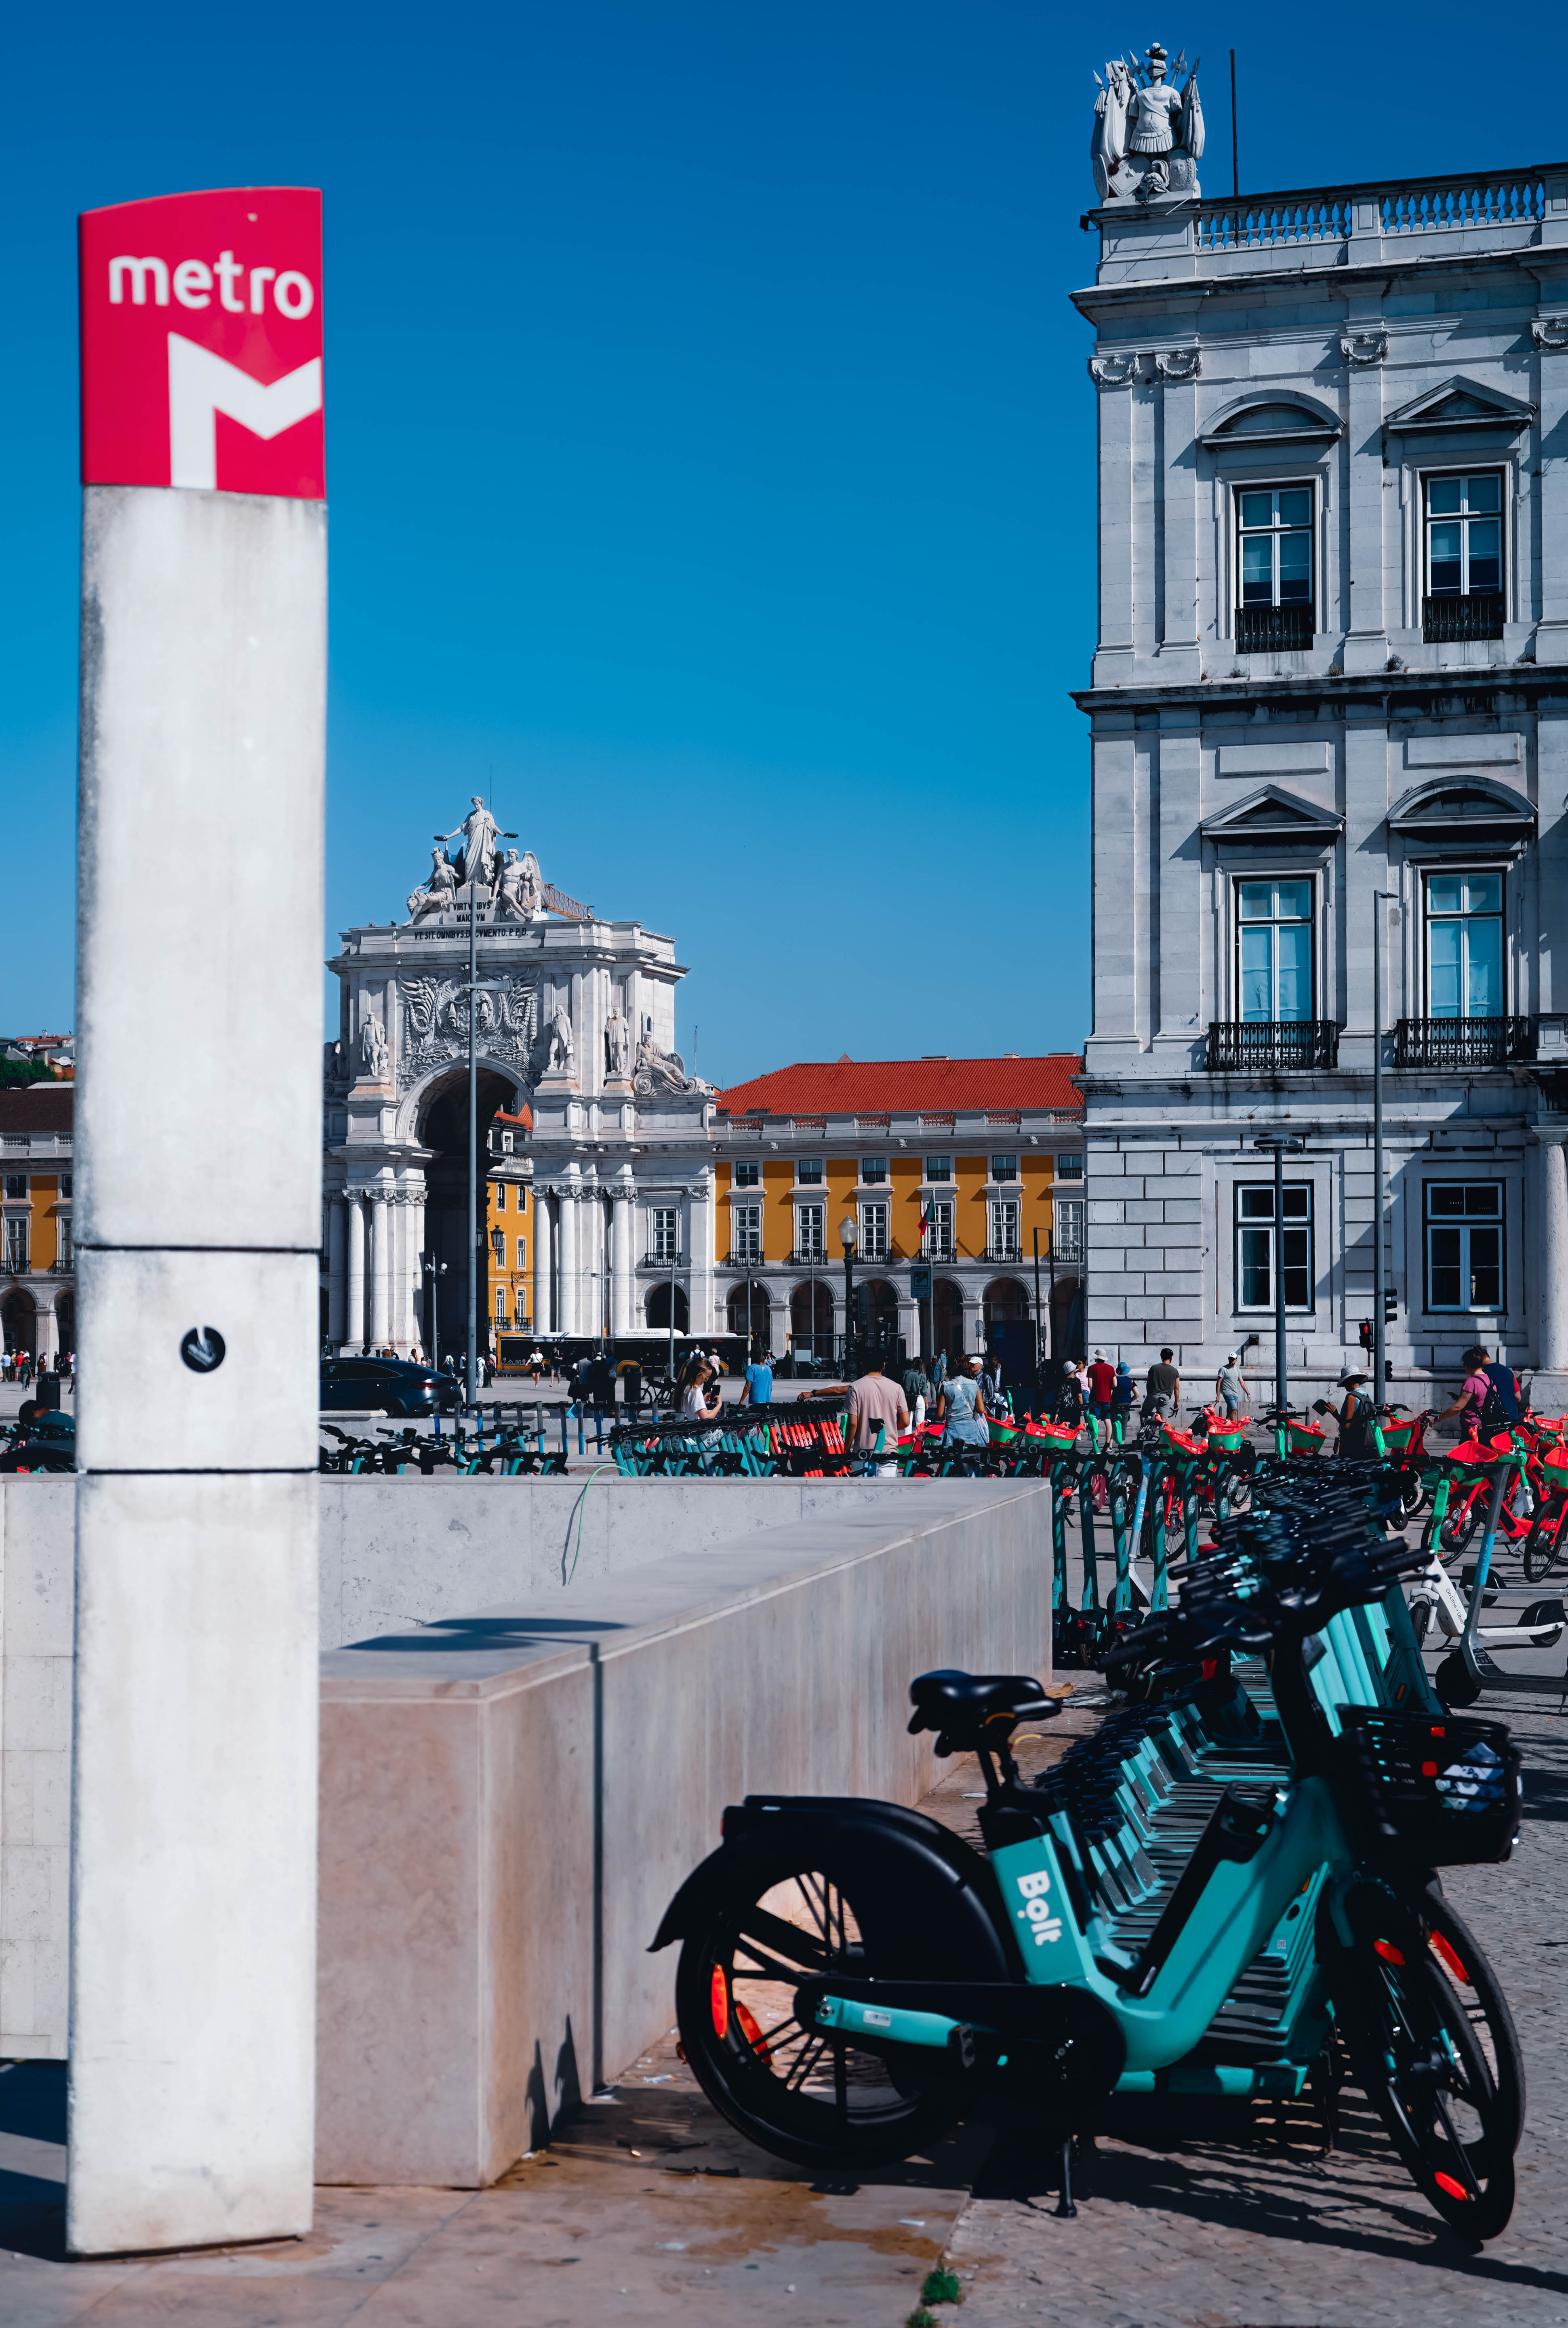
\includegraphics[width=\paperwidth,height=\paperheight]{src/Figures/Arriere_plan/Arriere_plan_Chap_2.jpg}
    }

% Rectangle
\AddToShipoutPictureBG*{
  \begin{tikzpicture}[remember picture,overlay]
    \node[fill=white, opacity=0.75, text width=\paperwidth, minimum height=12.25cm, anchor=north] 
    at ([yshift=-2cm]current page.north) {};
  \end{tikzpicture}
}

% Source
\AddToShipoutPictureFG*{
  \AtPageLowerRight{
    \raisebox{1cm}{
      \hspace{16cm}
      
\begin{tikzpicture}
        \node[fill=white, rounded corners=5pt, inner sep=5pt, align=center] {
          \tiny{Photography: \textcolor{blue}{Dylan Moinse (2023)}}
        };
      \end{tikzpicture}
    }
  }
}

    % ___________________________________________
    % Mini Table of Contents
    \cleardoublepage
    \setcounter{tocdepth}{2}
    % Redefine local table of contents title
    \renewcommand{\localcontentsname}{Table of Contents of Chapter~2}
\localtableofcontents

% Reset section numbering
\setcounter{section}{0}

%%%%%%%%%%%%%%%%%%%%%%%%%%%%%%%%
% Chapter 2
\newpage
\section*{Key Points of Chapter~2
    \label{chap2:graphical-abstract}
    }
    \markright{Chapter Preamble}{}

% \begin{figure}[h!]\vspace*{4pt}
%         \caption*{}
%         \label{graphical-abstract-chap2}
%         \centerline{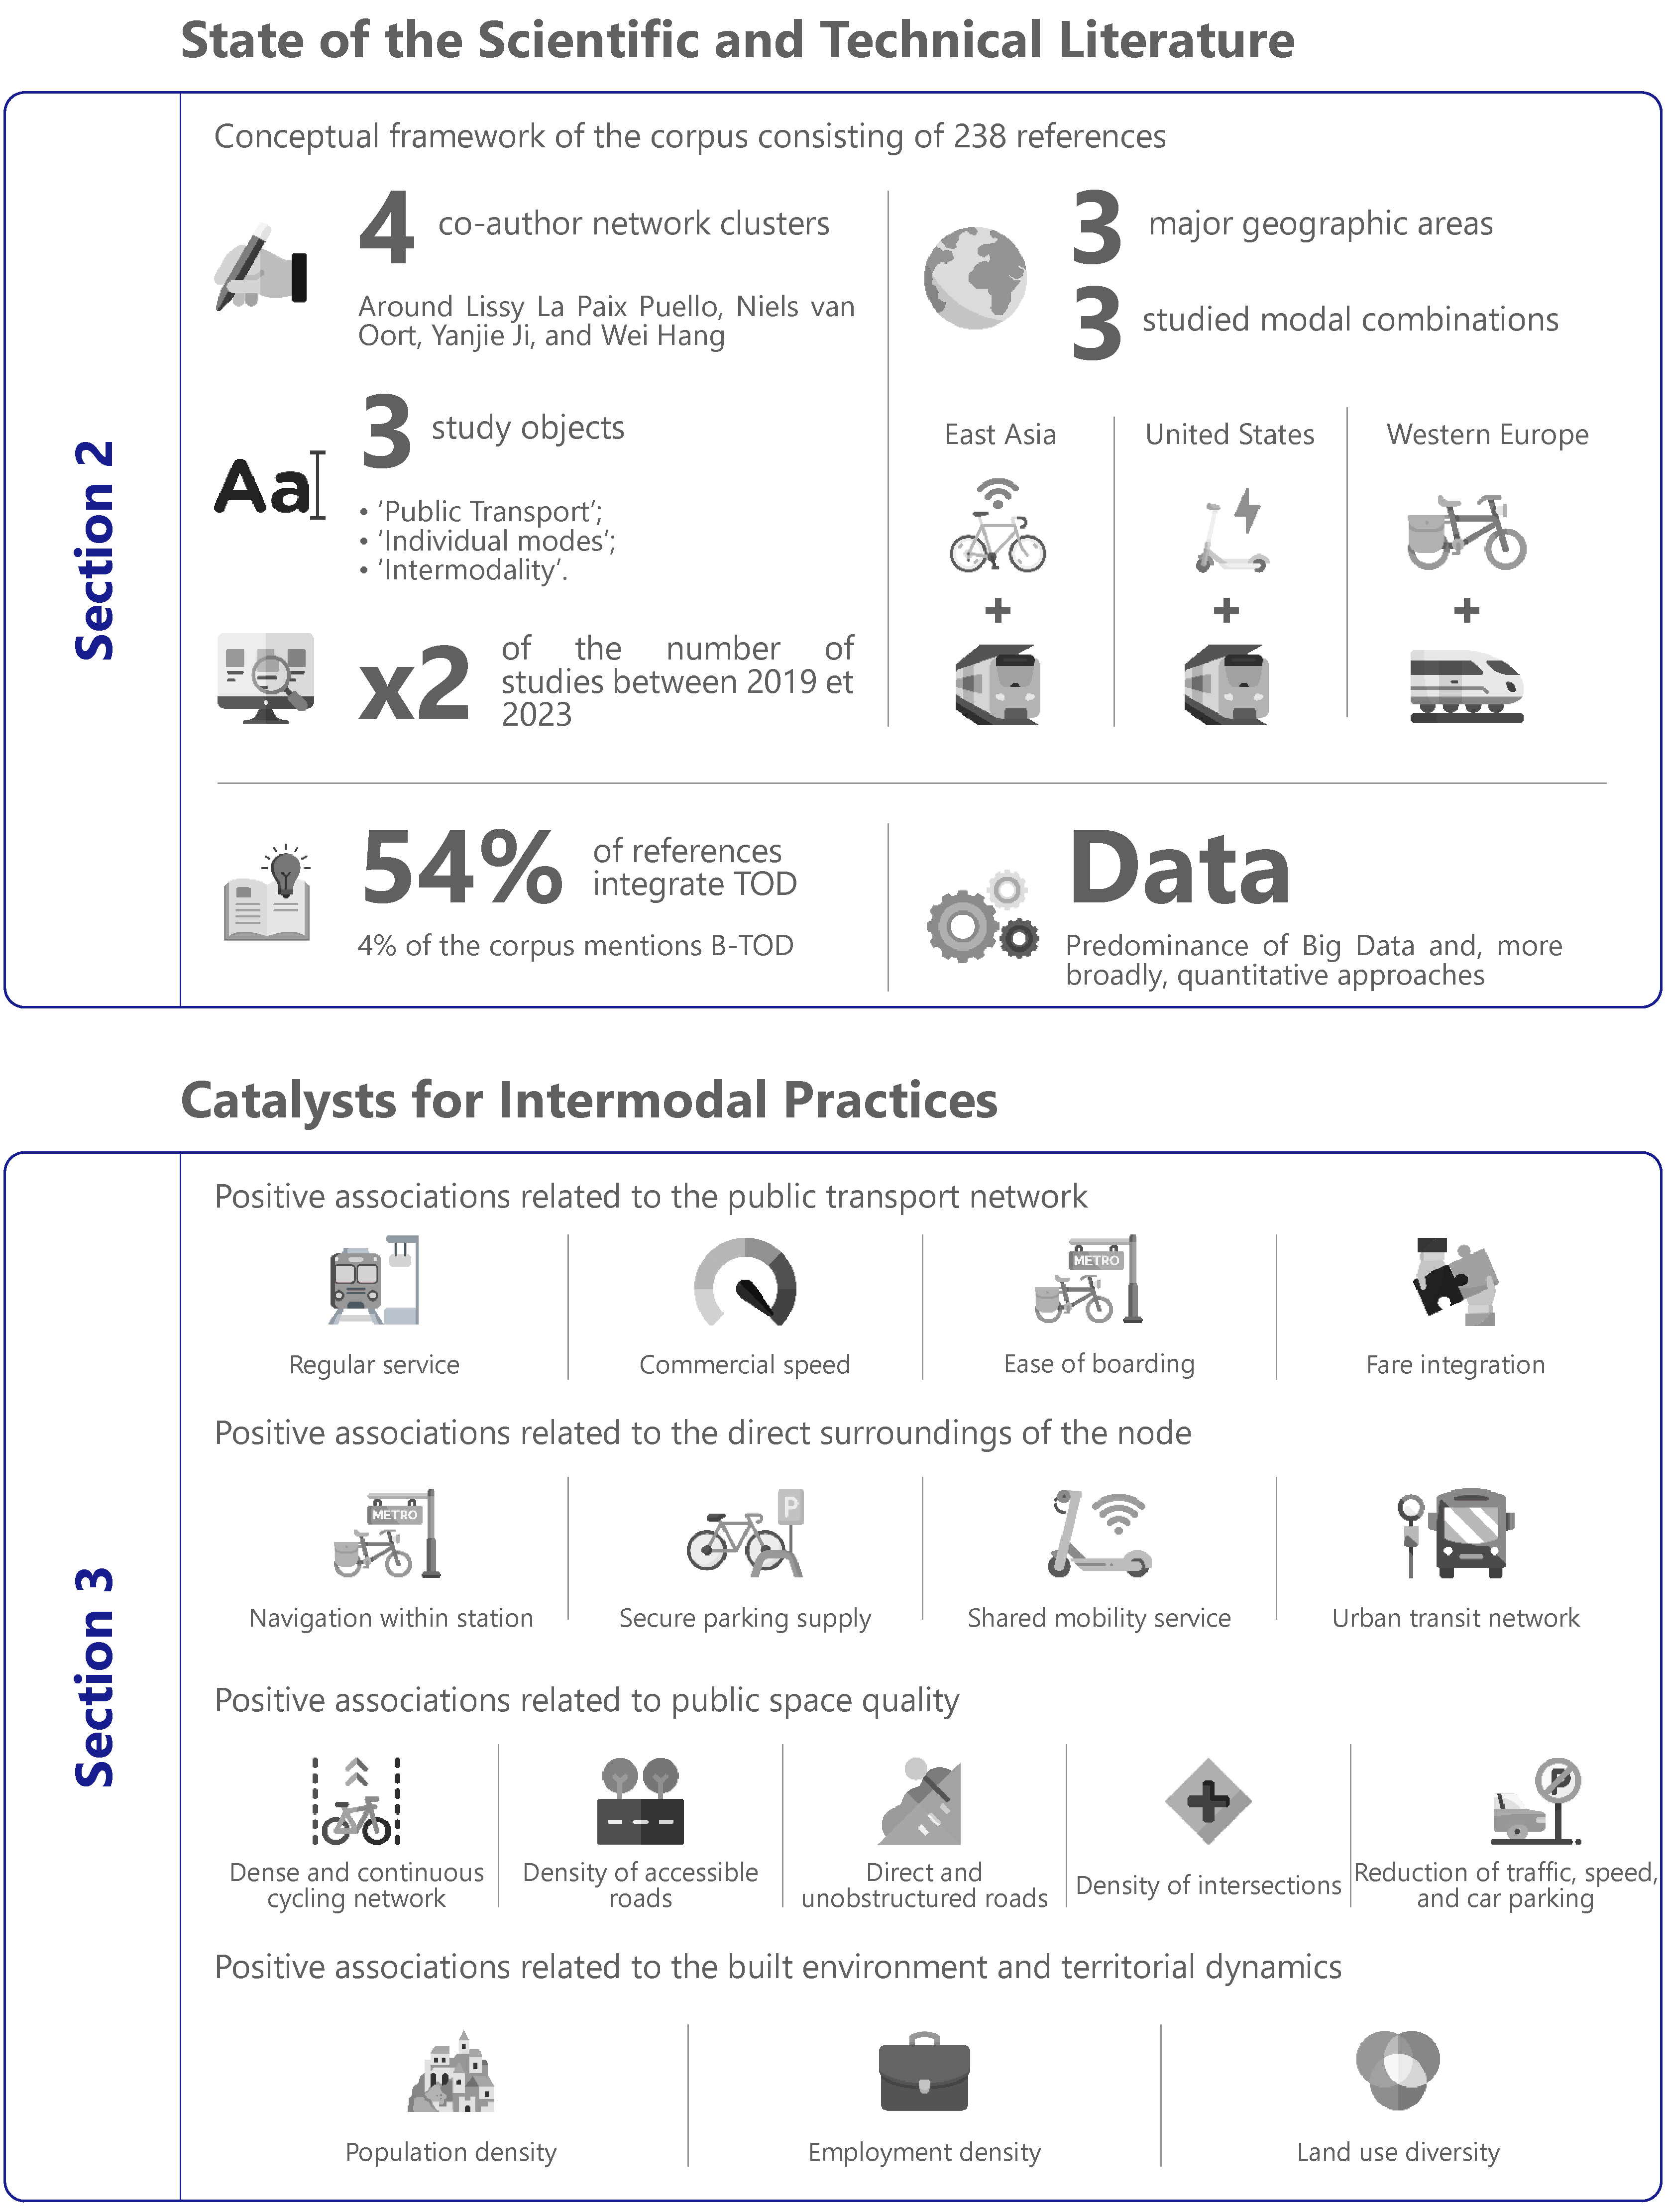
\includegraphics[width=1\columnwidth]{src/Figures/Graphical-abstract/EN_Graphical_abstract_chap2.pdf}}
%         \vspace{5pt}
%     \end{figure}

    % ___________________________________________
    % Preambule
    \newpage
    \begin{tcolorbox}[colback=white!5!white,
                      colframe=blue!75!blue,
                      title=
                      \bigskip
                      \center{\textbf{Preambule of Chapter~2}}
                      \\
                      \raggedright{\small{Chapter composed of \pagedifference{chap2:titre}{chap3:titre} pages, including \pagedifference{chap2:bibliographie}{chap3:titre} pages of bibliography}}
                      \bigskip]
\Large{\textbf{\textcolor{blue}{Abstract:}}}
    \\
    \small{
This chapter provides an overview of the current research on Transit-Oriented Development (TOD) promoting and supported by light individual mobility. This bibliometric study and bibliographical analysis are presented as a systematic literature review (SLR) compiling 238 scientific publications. The goal is to provide a state of knowledge on the B-TOD and M-TOD, with a preference for using the SLR due to its capacity to conduct an exhaustive analysis of the scientific literature on this research topic.%%Translated%%
    \\
The creation of this corpus involved selecting scientific articles, conference papers, book chapters, theses, and research reports in both English and French. These academic works were examined according to predefined criteria in order to identify all research addressing the intersection between light individual mobility and public transport (see \hyperref[chap2:protocole-methodologique-rsl]{Section~1}, page~\pageref{chap2:protocole-methodologique-rsl}).%%Translated%%
    \\
Initially, this bibliographic study examined the temporal, geographic, and institutional contexts influencing research on M-TOD, as well as the conceptual and methodological frameworks defined to assess this urban model (see \hyperref[chap2:analyse-documentation-rsl]{Section~2}, page~\pageref{chap2:analyse-documentation-rsl}). The analysis of the chronological and spatial distribution of the references revealed a growing interest in traveler intermodality, centered around three countries at a local scale, with modal combinations evolving over time. The adopted methodology tends towards developing geostatistical analyses and models, facilitated by the development of computing tools and Big Data.%%Translated%%
    \\
The third part of this chapter focuses on analyzing the lessons drawn from the studies reviewed, with particular attention to the various components of B-TOD and M-TOD, conceptualized under the term of the \Commas{7Ds} (see \hyperref[chap2:caracterisation-btod-environnement-urbain-choix-individuels]{Section~3}, page~\pageref{chap2:caracterisation-btod-environnement-urbain-choix-individuels}). The characterization of M-TOD revealed both similarities and divergences, highlighting a positive association with population and employment density, land use diversity, treatment of public spaces, and the quality of public transport services. Various impacts on mobility behaviors, mainly commuter-based, and on the environment were identified, such as a decrease in carbon footprint, improved accessibility to destinations for a larger portion of the population, as well as the existence of social inequalities in terms of accessibility.%%Translated%%
    \\
Finally, the SLR paves the way for a critical reading of the gaps in the scientific literature and the challenges of M-TOD (see \hyperref[chap2:conclusion]{chapter conclusion}, page~\pageref{chap2:conclusion}).%%Translated%%
    }
    \tcblower
\Large{\textbf{\textcolor{blue}{Keywords:}}}
    \\
    \small{
Bibliometric analysis;
Network analysis;
Socio-economic characteristics;
Urban characteristics;
Scientific mapping;
Mobility behaviors;
Impacts;
Critical reading of M-TOD;
International perspective;
Systematic literature review
    }
    \end{tcolorbox}

% ___________________________________________
% 2.*.
\newpage
\needspace{1\baselineskip} % Reserve space
\addcontentsline{toc}{section}{Introduction of Chapter~2}
\sectionheader{Introduction of Chapter~2}
\section*{Introduction of Chapter~2
    \label{chap2:introduction}
    }
    \markright{Introduction of Chapter~2}{}

    % Citation
    \begin{displayquote}
\Commas{\textsl{Next to innovations within transport modes, the strengths and weaknesses identified above also define the scope for transport mode combinations between transport modes. One such combination is between transport modes that give a relatively higher spatial access because of their speed with slower modes that have some other advantage.} [\dots] \foreignlanguage{english}{\textsl{Combinations between fast transit (such as trains) and non-motorized modes, particularly the bike, allow overall high door-to-door speed between virtually ubiquitous origin destinations. The train-bike combination is a particularly strong one: the train is much faster than other public transport, and the bike combines ubiquitous access with relatively high speeds (higher than walking but often also competitive with conventional buses or trams, and in certain environments even cars). In countries where both biking infrastructure and railway services are extensive~–~such as the Netherlands~–~this combination is so developed that it can be considered a transport mode in itself, and in many contexts directly competitive with the car.}} [\dots] \textsl{But also, the train-bike combination might integrate into a hybrid system which is both fast and flexible, and thus fully competitive with the car.} [\dots] \textsl{This type of multi-modal behaviour is now limited, but could become generalized in the future.} [\dots] \textsl{What if such a hybrid, highly adaptive behaviour and transportation system became dominant?}}

\textcolor{blue}{Luca} \textcolor{blue}{\textcite[80-81, 220]{bertolini_planning_2017}}\index{Bertolini, Luca|pagebf}. \foreignlanguage{english}{\textsl{Planning the Mobile Metropolis: Transport for People, Places and the Planet}}, Ed. Red Globe Press, Londres, 253~p. ISBN: \href{https://search.worldcat.org/fr/title/1004435849}{978-0-230-30877-0}
    \end{displayquote}

    % Introduction
\lettrine[lines=3, findent=8pt, nindent=0pt]{\lettrinefont T}{his} chapter aims to present the current state of knowledge addressing the redefinition of \acrfull{TOD} in connection with the renewed interest in light individual mobility, with the goal of defining the concept of \acrfull{B-TOD} expanded by light individual mobility. To collect, analyze, and contextualize research on this topic, a \acrfull{SLR} was conducted. Thus, only academic publications in English or French that focus on studying this form of \gls{intermodality}, from a geographical and urban perspective, were included in this bibliographic analysis.%%Translated%%

    % Justification B-TOD / M-TOD
In light of the potential of light individual mobility to expand the \gls{intermodal accessibility} of public transport nodes \textcolor{blue}{\autocite[118]{cottrell_transforming_2007}}\index{Cottrell, Wayne~D.|pagebf}, the underlying goal of this critical analysis of the scientific literature regarding the emerging concept of \acrfull{M-TOD} is to gather and better understand how this modal combination can promote urban design conducive to the development of alternative modes of transportation. Starting from the observation that the combination of public transport with light individual mobility, just like combined walking, represents the most effective form of integration \textcolor{blue}{\autocite[50]{sebban_complementarite_2003, yang_study_2013}}\index{Sebban, Annie-Claude|pagebf}\index{Yang, Rongrong|pagebf}\index{Yan, Hai|pagebf}\index{Xiong, Wen|pagebf}\index{Liu, Tao|pagebf}, both economically, socially, and environmentally—three dimensions valued by \acrshort{TOD} \textcolor{blue}{\autocite[85]{cervero_bike-and-ride_2013}}\index{Cervero, Robert|pagebf}\index{Caldwell, Benjamin|pagebf}\index{Cuellar, Jesus|pagebf}—the research question addressed by this \acrshort{SLR} is twofold. It seeks to justify the integration of light individual mobility into public transport systems as opposed to other forms of intermodality such as park-and-ride, while identifying the challenges inherent in the urban model of \acrshort{M-TOD}.%%Translated%%

    % Justification RSL
The value of conducting a \acrshort{SLR} lies in its ability to gather, assess, and synthesize existing knowledge on a complex research topic that blends two interdisciplinary objects of study, not only involving urban planning and mobility but also a multitude of disciplines related to urban systems, infrastructure, and populations. The innovative approach of the \acrshort{SLR} distinguishes itself from traditional literature reviews by its pursuit of enhanced objectivity, its goal of comprehensiveness, the formulation of specific questions, and the increased transparency of the steps involved in the process. While this method is primarily used in the exact sciences, the \acrshort{SLR} is proving its effectiveness in the \acrfull{HSS} through gradual adjustments. Therefore, developing such a method for an original and recent research topic offers several advantages. It allows for the identification and evaluation of existing studies, adopting a global and clear vision of the state of scientific knowledge, spotting emerging trends and the evolution of research, as well as identifying underexplored aspects. Consequently, the \acrshort{SLR} also helps to guide future research, as is the case with this doctoral research.%%Translated%%

    % Outline Announcement 1
We will first present in detail the methodological protocol for composing the academic corpus (\hyperref[chap2:protocole-methodologique-rsl]{Section~1}, page~\pageref{chap2:protocole-methodologique-rsl}), which will include the formulation of the research questions (\hyperref[chap2:formulation-questions-recherche]{Subsection~1.1}, page~\pageref{chap2:formulation-questions-recherche}), the documentary search strategy (\hyperref[chap2:strategie-recherche-documentaire]{Subsection~1.2}, page~\pageref{chap2:strategie-recherche-documentaire}), the processes of selecting scientific publications (\hyperref[chap2:selection-publications-scientifiques]{Subsection~1.3}, page~\pageref{chap2:selection-publications-scientifiques}) and extracting the collected data, as well as the examined aspects (\hyperref[chap2:extraction-donnees-aspects-consideres]{Subsection~1.4}, page~\pageref{chap2:extraction-donnees-aspects-consideres}).%%Translated%%

    % Outline Announcement 2
Once the methodology is presented, we will highlight the characteristics of the scientific literature and research practices on this topic (\hyperref[chap2:analyse-documentation-rsl]{Section~2}, page~\pageref{chap2:analyse-documentation-rsl}), through the analysis of metadata from the documentation (\hyperref[chap2:etat-litterature-scientifique-internationale-btod]{Subsection~2.1}, page~\pageref{chap2:etat-litterature-scientifique-internationale-btod}) and the conceptual and methodological frameworks of the bibliographic references (\hyperref[chap2:cadres-conceptuels-methodologiques]{Subsection~2.2}, page~\pageref{chap2:cadres-conceptuels-methodologiques}).%%Translated%%

    % Outline Announcement 3
The third part of this \acrshort{SLR} will be dedicated to a synthetic presentation of the \Commas{\acrfull{7Ds}} and the main lessons serving as guiding principles for the TOD (\hyperref[chap2:caracterisation-btod-environnement-urbain-choix-individuels]{Section~3}, page~\pageref{chap2:caracterisation-btod-environnement-urbain-choix-individuels}), by examining the association between the integration of light individual mobility and the influence of population density (\hyperref[chap2:densite-population]{Subsection~3.1}, page~\pageref{chap2:densite-population}), functional diversity (\hyperref[chap2:diversite-fonctionnelle]{Subsection~3.2}, page~\pageref{chap2:diversite-fonctionnelle}), the treatment of public spaces (\hyperref[chap2:traitement-espaces-publics]{Subsection~3.3}, page~\pageref{chap2:traitement-espaces-publics}), intermodal accessibility (\hyperref[chap2:accessibilite-intermodale]{Subsection~3.4}, page~\pageref{chap2:accessibilite-intermodale}), distances to and from transport nodes (\hyperref[chap2:distances-premiers-derniers-km]{Subsection~3.5}, page~\pageref{chap2:distances-premiers-derniers-km}), mobility demand management (\hyperref[chap2:gestion-demande-mobilite]{Subsection~3.6}, page~\pageref{chap2:gestion-demande-mobilite}), socio-demographic characteristics of users (\hyperref[chap2:sociodemographie-usagers]{Subsection~3.7}, page~\pageref{chap2:sociodemographie-usagers}), mobility behaviors (\hyperref[chap2:comportements-mobilite]{Subsection~3.8}, page~\pageref{chap2:comportements-mobilite}) and the impacts of these intermodal practices on mobility systems and urban systems (\hyperref[chap2:impacts-systemes-urbain-mobilite]{Subsection~3.9}, page~\pageref{chap2:impacts-systemes-urbain-mobilite}).%%Translated%%

    % Outline Announcement 4
In conclusion, we will suggest future research directions concerning the integration of light individual mobility into \acrshort{TOD}, which will contribute to this doctoral thesis (\hyperref[chap2:conclusion]{conclusion of Chapter~2}, page~\pageref{chap2:conclusion}).%%Translated%%

    % 2.1.
    \newpage
    \needspace{1\baselineskip} % Reserve space
    \sectionheader{Methodology of the Systematic Literature Review}
\section{Methodological Protocol of the Systematic Literature Review
    \label{chap2:protocole-methodologique-rsl}
    }
    
    % State of the Art SLR
The methodological procedure underlying the development of a \acrshort{SLR} is constantly evolving due to its relatively recent emergence in the fields of \acrshort{HSS} and ongoing discussions about the methodological limitations associated with it. The \acrshort{SLR} conducted in this chapter follows the techniques outlined in the reference article dedicated to the execution of a thematic and qualitative \acrshort{SLR} in a medical scientific journal, written by \textcolor{blue}{\textcite[3-7]{thomas_methods_2008}}\index{Thomas, James|pagebf}\index{Harden, Angela|pagebf}. Considering the nuances in performing an \acrshort{SLR} across disciplines \textcolor{blue}{\autocite[738]{padeiro_transit-oriented_2019}}\index{Padeiro, Miguel|pagebf}\index{Louro, Ana|pagebf}\index{Costa, Nuno Marques de|pagebf}, the developed methodological protocol is based on lessons drawn from various \acrshort{SLR}\textcolor{blue}{s} examining \acrshort{TOD} and light individual mobility. The method used draws on techniques and reflections from various \acrshort{SLR}\textcolor{blue}{s}, one focusing on the links between \acrshort{TOD} and gentrification \textcolor{blue}{\autocite[738]{padeiro_transit-oriented_2019}}\index{Padeiro, Miguel|pagebf}\index{Louro, Ana|pagebf}\index{Costa, Nuno Marques de|pagebf}, and another on the integration of light individual mobility with public transportation systems \textcolor{blue}{\autocite[4]{oeschger_micromobility_2020}}\index{Oeschger, Giulia|pagebf}\index{Carroll, Páraic|pagebf}\index{Caulfield, Brian|pagebf}. Several existing literature reviews also guided the design of our \acrshort{SLR}, particularly those examining bicycles and electric micromobility \textcolor{blue}{\autocite[3]{sengul_impacts_2021}}\index{Sengül, Buket|pagebf}\index{Mostofi, Hamid|pagebf}, electric scooter services \textcolor{blue}{\autocite[4]{bozzi_shared_2021}}\index{Bozzi, Alberica Domitilla|pagebf}\index{Aguiléra, Anne|pagebf}, the choice of cycling routes \textcolor{blue}{\autocite[2]{pritchard_revealed_2018}}\index{Pritchard, John~P.|pagebf}, and the use of \textsl{Big Data} in mobility \textcolor{blue}{\autocite[36]{neilson_systematic_2019}}\index{Neilson, Alex|pagebf}\index{Indratmo|pagebf}\index{Daniel, Ben|pagebf}\index{Tjandra, Stevanus|pagebf}.%%Translated%%

    % Selection
Moreover, this bibliographic research is inspired by the methodological guide intended to produce a literature review in the fields of urban planning and mobility, as adapted by the US national academic organization \textcolor{blue}{\textcite{transportation_research_board_of_the_national_academies_literature_2015}}\index{Transportation Research Board@\textsl{Transportation Research Board}|pagebf}. This report notably identifies six main steps to constitute an \acrshort{SLR}: defining the research subject (i), selecting appropriate libraries and bibliographic databases for the defined subject (ii), formulating an expression using keywords (iii), defining relationships between terms to develop an advanced search (iv), checking the collection of texts gathered (v), and organizing the data for analysis (vi) \textcolor{blue}{\autocite[2-18]{transportation_research_board_of_the_national_academies_literature_2015}}\index{Transportation Research Board@\textsl{Transportation Research Board}|pagebf}. Furthermore, the process of selecting scientific publications for this \acrshort{SLR} embraces the three stages established by \textcolor{blue}{\textcite[2544]{jain_systematic_2020}}\index{Jain, Deepshikha|pagebf}\index{Singh, Ekta|pagebf}\index{Ashtt, Rashmi|pagebf}:
    \begin{customitemize}
        \item The initial exclusion phase involves analyzing the metadata from bibliographic references, including the title, abstract, and associated keywords, to assess their relevance to the research topic;
        \item The intermediate exclusion phase involves critical reading of the introduction and conclusion of each retained document to further filter publications that align with the research objectives set in the \acrshort{SLR};
        \item The final exclusion phase engages a full reading of the studies included in the \acrshort{SLR} to ensure the quality of the selection process.
    \end{customitemize}
Following these three sequences, the inclusion process ensures a methodical approach to identifying relevant academic sources related to the specified research topic.%%Translated%%

    % Advantages of SLR
Compared to a conventional literature review, the \acrshort{SLR} acquires the status of being \Commas{systematic} when it is structured around a formulated research question, the identification of relevant works in line with the defined topic, and a clear explanation of the methodology followed. In this sense, the \acrshort{SLR} holds several comparative advantages \textcolor{blue}{\autocite[2]{transportation_research_board_of_the_national_academies_literature_2015}}\index{Transportation Research Board@\textsl{Transportation Research Board}|pagebf}:
    \begin{customitemize}
        \item The problem-solving capacity enabled by the comprehensive coverage of existing knowledge on a specific topic;
        \item The confrontation of previous and competing studies, facilitating the understanding of the existing academic discourse;
        \item The validation of the research methods applied by questioning the reliability of the chosen approaches;
        \item The confirmation of the necessity to continue research by highlighting emerging study areas;
        \item The guidance of research efforts by providing perspectives that shed light on the current state of knowledge and suggest promising directions for future research initiatives.
    \end{customitemize}
With these advantages, the \acrshort{SLR} establishes a solid foundation to probe the scientific literature, contributing to greater methodological rigor, a fine analysis of existing research, and a roadmap to guide subsequent studies.%%Translated%%

    % 2.1.1.
    \needspace{1\baselineskip} % Reserve space
\subsection{Formulation of Research Questions
    \label{chap2:formulation-questions-recherche}
    }
    
    % Questions and objectives
The primary goal of this \acrshort{SLR} is to provide a deep understanding of the existing knowledge and practices related to urban planning oriented towards public transportation, supported by light individual mobility, while identifying the factors that facilitate or hinder the implementation of this urban model and assessing its effects on mobility and territories. In this regard, the \acrshort{SLR} aims to first examine and discuss the role of the bicycle within the planning model. Although the integration of this mode of transport was considered from the conceptualization of \acrshort{TOD}, its potential seems to remain underexplored. It is with this perspective that this literature review seeks to characterize its iteration, known as \acrshort{M-TOD}. Additionally, we aim to update it by incorporating the exploration of emerging \gls{micromobility} options. These, due to their innovative nature, are likely to interact with and transform the foundations of \acrshort{M-TOD} in turn.%%Translated%%

    % Research Questions
The following reading grid, centered around six research questions, guides the \acrshort{SLR}:
    \begin{customitemize}
        \item What urban factors and public policies promote the integration of bicycles and micromobility options into public transport systems? Conversely, does this form of mobility influence territorial configurations?
        \item What are the effects of this modal combination in terms of economic development, social cohesion, and environmental sustainability?
        \item Is there a relevant perimeter to define a transit-oriented development area based on light individual mobility? Does the size of these influence areas vary according to certain parameters?
        \item What urban planning practices and governance models prove to be innovative and effective in promoting such urban development?
        \item Can the \acrshort{M-TOD} be considered an internationally recognized and replicable urban model?
        \item What are the main challenges to be addressed when reflecting on and applying an \acrshort{M-TOD} strategy?
    \end{customitemize}%%Translated%%

    % 2.1.2.
    \needspace{1\baselineskip} % Reserve space
\subsection{Search Strategy for the Literature Review
    \label{chap2:strategie-recherche-documentaire}
    }

    % Online Research
The initial data collection phase is carried out using online searches, utilizing bibliographic databases offering transdisciplinary coverage. This documentation collection step ensures the capture and listing of a comprehensive corpus of bibliographic references from scientific literature and grey literature
    \footnote{~
        In this context, scientific literature refers to peer-reviewed academic publications, including articles published in scientific journals, conference proceedings, book chapters, and research theses. Grey literature, as defined by \acrfull{AFNOR} and the Luxembourg Convention on Grey Literature, includes \Commas{\textsl{typed or printed documents, often provisional in nature, reproduced and distributed in fewer than a thousand copies, outside the commercial publishing and distribution channels}}~\textcolor{blue}{\autocite[30]{schopfel_comprendre_2015}}\index{Schöpfel, Joachim|pagebf}. Grey literature encompasses \Commas{\textsl{what is produced by all levels of government, universities, businesses, and industry, in printed or electronic form, but not controlled by commercial publishing}}~\textcolor{blue}{\autocite{national_grey_literature_collection_luxembourg_nodate}}\index{National Grey Literature Collection|pagebf}. Recently, \textcolor{blue}{Joachim} \textcolor{blue}{\textcite[9]{schopfel_vers_2012}}\index{Schöpfel, Joachim|pagebf} proposed a renewed definition of this type of literature, considering it as \Commas{\textsl{a document produced by government, administration, education and research, business and industry, in printed or electronic form, protected by intellectual property rights, of sufficient quality to be collected and preserved by a library or institutional archive, and not controlled by commercial publishing}}.
}. In this \acrshort{SLR}, online searches include scientific articles, conference proceedings, book chapters, master's or doctoral research theses, and public research reports. However, they exclude, among others, scientific preprints, technical or policy documents, private study reports, public statements, or newsletters. It is worth noting that the bibliographic inventory related to \acrshort{M-TOD} was initially created between December 3 and 8, 2021. Later, due to the emerging nature of this topic, an update to the data collection was carried out between April 10 and 13, 2023, to include the most recent publications.%%Translated%%

    % Online Research Step
The data collection for this \acrshort{SLR} was carried out through an \acrfull{EN~Search}, or \(S_{EN}\), and an \acrfull{FR~Search}, or \(S_{FR}\), using various online platforms that have solid recognition in the academic sphere. The academic resources cited below were selected due to their extensive coverage, accessibility, and reliability. Furthermore, these digital databases facilitate the identification, indexing, and export of a wide range of scientific references to reference management software, especially thanks to their integrated advanced search tools.%%Translated%%

    % Figure RSL - Sampling
    \begin{figure}[h!]\vspace*{4pt}
        \caption{Flow diagram representing the process of selecting scientific publications integrated into the systematic literature review.}
        \label{fig-chap2:diagramme-flux-selection-publications-rsl}
        \centerline{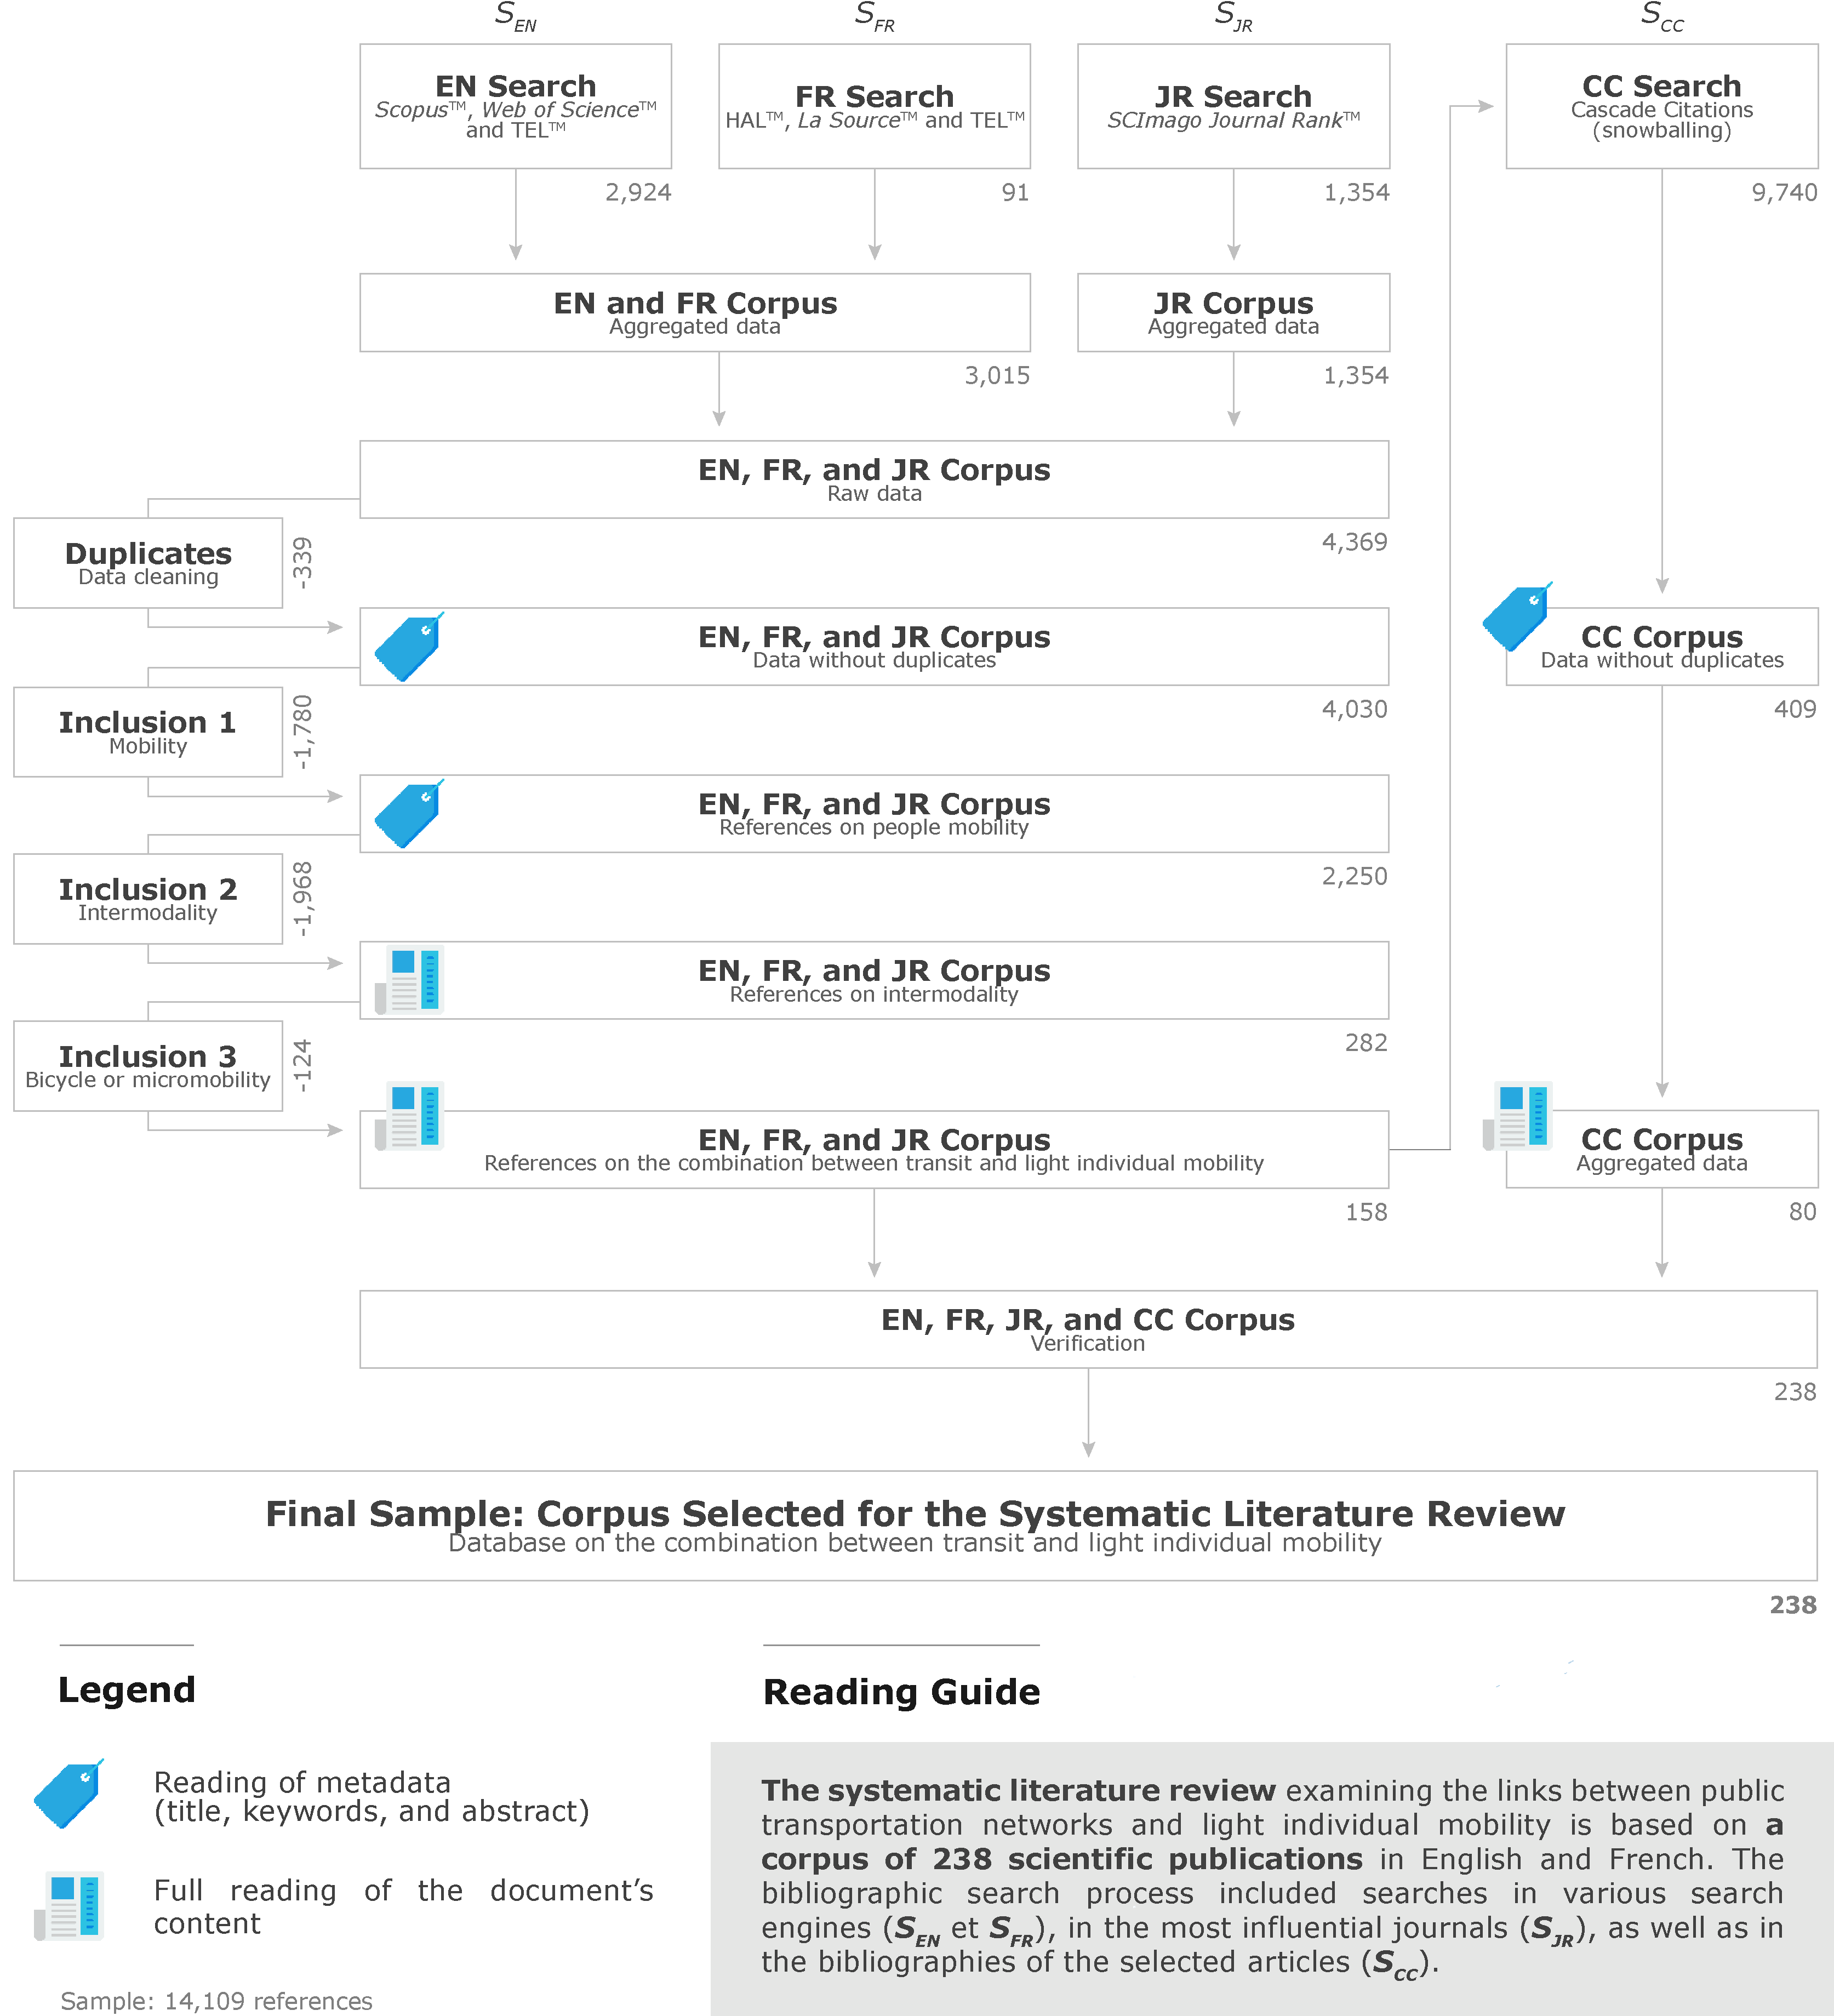
\includegraphics[width=1\columnwidth]{src/Figures/Chap-2/EN_RSL_Diagramme_flux_selection_publications.pdf}}
        \vspace{5pt}
        \begin{flushright}\scriptsize{
        Author: \textcolor{blue}{Dylan Moinse (2023)}
        }\end{flushright}
    \end{figure}

    % Searches EN+FR
In the first case, we queried the \Marque{Scopus} and \Marque{Web of Science} databases\footnote{~
    \textsl{Scopus} (\url{www.scopus.com}) and \textsl{Web of Science} (\url{www.webofscience.com}) are online bibliographic platforms commonly used in academic research. \textsl{Scopus} is developed by \Marque{Elsevier}, a company specializing in scientific publishing, while \textsl{Web of Science} is a collection of academic works managed by \Marque{Clarivate Analytics}.
}. Additionally, the \Marque{TEL} server\footnote{~
    \textsl{theses.fr} (\url{www.theses.fr}) is a platform for doctoral theses, regularly providing online access to academic resources produced by doctoral students.
} was consulted to expand the search to doctoral theses submitted in English. In the second phase, the bibliographic research in French relied on the \Marque{HAL} portal\footnote{~
    \textsl{Hyper Article en Ligne} (\url{https://hal.science/}) is an open archive portal that facilitates the deposit, dissemination, and consultation of scientific documents. This portal was developed by the \acrfull{CCSD} of the \acrfull{CNRS}. \textsl{HAL} allows researchers and institutions to disseminate their research freely to facilitate open access and visibility.
}, the \Marque{La Source} platform\footnote{~
    \textsl{La Source} (\url{https://bibliotheque.enpc.fr}) is the online library developed by the \textsl{École des Ponts Paristech}, designed to facilitate access to scientific resources available on its online platform.
}, and again on the \textsl{TEL} server. The \Commas{\acrshort{EN~Search}} resulted in the compilation of 2,924 scientific publications, while the \Commas{\acrshort{FR~Search}} added 91 references, after updating the collection in April 2023. Thus, this first step of the online search formed a corpus of 3,015 documents, referred to as the \Commas{EN and FR Corpus} (see \hyperref[fig-chap2:diagramme-flux-selection-publications-rsl]{Figure~\ref{fig-chap2:diagramme-flux-selection-publications-rsl}}, page~\pageref{fig-chap2:diagramme-flux-selection-publications-rsl}).%%Translated%%

    % Table scientific journals
% Table of station area types
%%Translated%%
        \begin{table}[h!]
    \centering
    \renewcommand{\arraystretch}{1.5}
    \resizebox{\columnwidth}{!}{
    \begin{tabular}{p{0.07\columnwidth}p{0.1\columnwidth}p{0.7\columnwidth}p{0.13\columnwidth}}
        %\hline
    \rule{0pt}{15pt} \small{\textbf{\textcolor{blue}{Rank}}} & \small{\textbf{\textcolor{blue}{Label}}} & \small{\textbf{\textcolor{blue}{Scientific Journal}}} & \small{\textbf{\textcolor{blue}{\acrshort{SJR} Index}}}\\
        \hline
    \multicolumn{4}{l}{\small{\textbf{\textcolor{blue}{Transport (2023)}}}}\\
\small{1} & \small{\(SMG_{T1}\)} & \small{\textsl{Analytic Methods in Accident Research}} & \small{4.8}\\
\small{2} & \small{\(SMG_{T2}\)} & \small{\textsl{Tourism Management}} & \small{3.4}\\
\small{3} & \small{\(SMG_{T3}\)} & \small{\textsl{Transportation Research Part B: Methodological}} & \small{3.4}\\
\small{4} & \small{\(SMG_{T4}\)} & \small{\textsl{Journal of Travel Research}} & \small{3.3}\\
\small{5} & \small{\(SMG_{T5}\)} & \small{\textsl{Transportation Research Part C: Emerging Technologies}} & \small{3.2}\\
\small{6} & \small{\(SMG_{T6}\)} & \small{\textsl{Transport Reviews}} & \small{3.1}\\
\small{7} & \small{\(SMG_{T7}\)} & \small{\textsl{Transportation Research Part E: Logistics and Transportation}} & \small{2.8}\\
\small{8} & \small{\(SMG_{T8}\)} & \small{\textsl{Transportation Science}} & \small{2.8}\\
\small{9} & \small{\(SMG_{T9}\)} & \small{\textsl{Journal of Public Transportation}} & \small{2.3}\\
\small{10} & \small{\(SMG_{T10}\)} & \small{\textsl{Transportation Research, Part A: Policy and Practice}} & \small{2.2}\\
        \hline
    \multicolumn{4}{l}{\small{\textbf{\textcolor{blue}{Urban Studies (2023)}}}}\\
\small{1} & \small{\(SMG_{U1}\)} & \small{\textsl{Nature Sustainability}} & \small{5.8}\\
\small{2} & \small{\(SMG_{U2}\)} & \small{\textsl{Journal of Urban Economics}} & \small{2.8}\\
\small{3} & \small{\(SMG_{U3}\)} & \small{\textsl{Journal of Public Transportation}} & \small{2.3}\\
\small{4} & \small{\(SMG_{U4}\)} & \small{\textsl{Transportation Research Interdisciplinary Perspectives}} & \small{2.1}\\
\small{5} & \small{\(SMG_{U5}\)} & \small{\textsl{Landscape and Urban Planning}} & \small{1.9}\\
\small{6} & \small{\(SMG_{U6}\)} & \small{\textsl{Urban Studies}} & \small{1.9}\\
\small{7} & \small{\(SMG_{U7}\)} & \small{\textsl{International Journal of Urban and Regional Research}} & \small{1.9}\\
\small{8} & \small{\(SMG_{U8}\)} & \small{\textsl{Journal of the American Planning Association}} & \small{1.8}\\
\small{9} & \small{\(SMG_{U9}\)} & \small{\textsl{Computers, Environment and Urban Systems}} & \small{1.7}\\
\small{10} & \small{\(SMG_{U10}\)} & \small{\textsl{Cities}} & \small{1.7}\\
        \hline
        \end{tabular}}
    \caption{List of scientific journals ranked by the \Marque{SCImago Journal Rank}, included in the \Commas{JR~Search} of the systematic literature review.}
    \label{table-chap2:revues-scientifiques-rsl}
        \vspace{5pt}
        \begin{flushleft}\scriptsize{
        \textcolor{blue}{Note:} The journal \textsl{Journal of Public Transportation} appears in both rankings (\(SMG_{T9}\) and \(SMG_{U3}\)).
        \\
        \textcolor{blue}{Reading:} The twenty most influential transport and urban studies journals were individually reviewed to identify relevant scientific publications related to the topic of our systematic literature review.
        }\end{flushleft}
        \begin{flushright}\scriptsize{
        Data source: \Marque{SCImago Journal Rank}~\textcolor{blue}{\autocite{sjr_scimago_2023}}
        }\end{flushright}
        \end{table}%%Translated%%

    % CR Search
Despite the variety of scientific publications accessible through the aforementioned documentary databases and servers, their advanced search features may prove insufficient to cover the entire field of study, due to constraints in search algorithms and the formulation of the defined keywords. To overcome the limitations of the advanced search tools available in these electronic sources, the search strategy for this \acrshort{SLR} was enhanced by a second stage of bibliographic exploration, involving the direct consultation of peer-reviewed scientific journals. This manual bibliographic search, referred to as \acrfull{JR~Search}, or \(S_{JR}\), follows the method employed by \textcolor{blue}{\textcite[738]{padeiro_transit-oriented_2019}}\index{Padeiro, Miguel|pagebf}\index{Louro, Ana|pagebf}\index{Costa, Nuno Marques de|pagebf}. To this end, we consulted an international classification of scientific journals by discipline, provided by the online platform \textsl{SJR}\footnote{~
    \textsl{SJR} is a platform developed by \Marque{SCImago Lab}, providing several performance indicators to evaluate peer-reviewed journals, notably the \acrfull{SJR} index, which measures the reputation and scientific impact of journals. The \textsl{SJR} tool uses the \Marque{PageRank} algorithm from \Marque{Google} to determine the quality and influence of a journal, considering the number of citations received by each article, the quality of the citing journals, and the relevant scientific disciplines. The \acrshort{SJR} index is an alternative to the \acrfull{h-index} and offers a more nuanced perspective on a journal's impact by considering both the quantity and quality of citations received.
} that established the \acrfull{SJR} index to measure the quality and influence of a journal. Based on this ranking, we found it relevant to consult the top ten scientific journals in the fields of \Commas{transportation} and \Commas{urban studies,} resulting in a \Commas{CR Corpus} of 1,354 publications (see \hyperref[table-chap2:revues-scientifiques-rsl]{Table~\ref{table-chap2:revues-scientifiques-rsl}}, page~\pageref{table-chap2:revues-scientifiques-rsl}). After cleaning the data by removing duplicates and revising in 2023, the \Commas{EN, FR, and CR Corpus} includes a total of 4,030 bibliographic references (see \hyperref[fig-chap2:diagramme-flux-selection-publications-rsl]{Figure~\ref{fig-chap2:diagramme-flux-selection-publications-rsl}}, page~\pageref{fig-chap2:diagramme-flux-selection-publications-rsl}).%%Translated%%

    % 2.1.3.
    \needspace{1\baselineskip} % Reserve space
\subsection{Selection Process of Scientific Publications
    \label{chap2:selection-publications-scientifiques}
    }

    % Table expression
% Search expression table
%%Translated%%
        \begin{table}[h!]
    \centering
    \renewcommand{\arraystretch}{1.5}
    \resizebox{\columnwidth}{!}{
    \begin{tabular}{p{0.5\columnwidth}p{0.5\columnwidth}}
        %\hline
    \rule{0pt}{15pt} \small{\textbf{\textcolor{blue}{\acrshort{EN~Search}}}} & \small{\textbf{\textcolor{blue}{\acrshort{FR~Search}}}}\\
        \hline
    \multicolumn{2}{l}{\small{\textbf{\textcolor{blue}{Dimension related to public transport}}}}\\
\small{all=(\textbf{\Commas{\textsl{Transit-Oriented Development}}} or \textbf{\Commas{\textsl{Public Transport}}} or \textbf{\Commas{\textsl{Transit}}} or \textbf{\Commas{\textsl{Rail}}} or \textbf{\Commas{\textsl{Train}}} or \textbf{\Commas{\textsl{Metro}}} or \textbf{\Commas{\textsl{Tram}}} or \textbf{\Commas{\textsl{Bus}}})} & \small{all=(\textbf{\Commas{\textsl{Transit-Oriented Development}}} or \textbf{\Commas{\textsl{Urbanisme orienté}}} or \textbf{\Commas{\textsl{Public Transport}}} or \textbf{\Commas{\textsl{Collective Transport}}} or \textbf{\Commas{\textsl{Rail}}} or \textbf{\Commas{\textsl{Train}}} or \textbf{\Commas{\textsl{Railway}}} or \textbf{\Commas{\textsl{Metro}}} or \textbf{\Commas{\textsl{Tram}}} or \textbf{\Commas{\textsl{BRT}}} or \textbf{\Commas{\textsl{Bus}}})}\\
        \hdashline
    \multicolumn{2}{l}{\small{\textbf{\textcolor{blue}{Boolean Operator}}}}\\
 \multicolumn{2}{l}{\small{and}}\\
        \hdashline
    \multicolumn{2}{l}{\small{\textbf{\textcolor{blue}{Dimension related to light individual mobility}}}}\\
\small{all=(\textbf{\Commas{\textsl{Micromobility}}} or \textbf{\Commas{\textsl{Micro-Mobility}}} or \textbf{\Commas{\textsl{Bicycle*}}} or \textbf{\Commas{\textsl{Bike*}}} or \textbf{\Commas{\textsl{Bike-And-Ride}}} or \textbf{\Commas{\textsl{Cycling}}} or \textbf{\Commas{\textsl{E-Scooter*}}} or \textbf{\Commas{\textsl{Scooter*}}} or \textbf{\Commas{\textsl{Device*}}})} & \small{all=(\textbf{\Commas{\textsl{Micro-mobility*}}} or \textbf{\Commas{\textsl{Micromobility*}}} or \textbf{\Commas{\textsl{Bicycle*}}} or \textbf{\Commas{\textsl{Bike*}}} or \textbf{\Commas{\textsl{Active Mode*}}} or \textbf{\Commas{\textsl{Soft Mode}}} or \textbf{\Commas{\textsl{Cycle*}}} or \textbf{\Commas{\textsl{Cyclable}}} or \textbf{\Commas{\textsl{Scooter*}}} or \textbf{\Commas{\textsl{Micro-vehicle*}}})}\\
        \hdashline
    \multicolumn{2}{l}{\small{\textbf{\textcolor{blue}{Boolean Operator}}}}\\
\multicolumn{2}{l}{\small{and}}\\
        \hdashline
    \multicolumn{2}{l}{\small{\textbf{\textcolor{blue}{Dimension related to intermodality-passenger(s)}}}}\\
\small{all=(\textbf{\Commas{\textsl{Intermodal*}}} or \textbf{\Commas{\textsl{Combination}}} or \textbf{\Commas{\textsl{*Last Mile}}} or \textbf{\Commas{\textsl{First Mile*}}} or \textbf{\Commas{\textsl{FLM}}} or \textbf{\Commas{\textsl{Feeder}}} or \textbf{\Commas{\textsl{Transfer}}} or \textbf{\Commas{\textsl{Relation*}}} or \textbf{\Commas{\textsl{Integration}}} or \textbf{\Commas{\textsl{Catchment}}} or \textbf{\Commas{\textsl{Isochrone*}}} or \textbf{\Commas{\textsl{Buffer}}} or \textbf{\Commas{\textsl{Service Coverage}}} or \textbf{\Commas{\textsl{Shed*}}} or \textbf{\Commas{\textsl{Station Area*}}} or \textbf{\Commas{\textsl{Access}}} or \textbf{\Commas{\textsl{Egress}}})} & \small{all=(\textbf{\Commas{\textsl{Intermodal*}}} or \textbf{\Commas{\textsl{Combination}}} or \textbf{\Commas{\textsl{First* Mile*}}} or \textbf{\Commas{\textsl{Last* Mile*}}} or \textbf{\Commas{\textsl{Feeder}}} or \textbf{\Commas{\textsl{Pre-access}}} or \textbf{\Commas{\textsl{Diffusion}}} or \textbf{\Commas{\textsl{Post-access}}} or \textbf{\Commas{\textsl{Interaction*}}} or \textbf{\Commas{\textsl{Integration}}} or \textbf{\Commas{\textsl{Catchment Area}}} or \textbf{\Commas{\textsl{Influence Area}}} or \textbf{\Commas{\textsl{Isochrone*}}} or \textbf{\Commas{\textsl{Station Area*}}})}\\
        \hline
        \end{tabular}}
    \caption{Search expression of keywords in English and French, covering three thematic categories, for the systematic literature review.}
    \label{table-chap2:expression-recherche-rsl}
        \vspace{5pt}
        \begin{flushleft}\scriptsize{
        \textcolor{blue}{Note:} The asterisk (*) provides greater flexibility to terms by allowing a wider scope in advanced searches, accommodating additional characters before or after the word. As a result, this symbol includes plural forms or variants of terms, among other possibilities.
        \\
        \textcolor{blue}{Reading:} The bibliographic search formula relies on three conditions: lexical presence referring to public transport, light individual mobility, and intermodality.
        }\end{flushleft}
        \begin{flushright}\scriptsize{
        Author: \textcolor{blue}{Dylan Moinse (2023)}
        }\end{flushright}
        \end{table}%%Translated%%

    % Boolean operators
The identification of academic works related to \acrshort{M-TOD} was carried out by using the specified electronic databases. A search expression was defined based on three distinct categories, namely public transport (i), light individual mobility (ii), and intermodal travel (iii). Considering the terminological variations of each category, the expression was enhanced with the integration of boolean operators \Commas{and} (\textsl{and}) and \Commas{or} (\textsl{or}) to cover the three classes of keywords (see \hyperref[table-chap2:expression-recherche-rsl]{Table~\ref{table-chap2:expression-recherche-rsl}}, page~\pageref{table-chap2:expression-recherche-rsl}). The designation of keywords was facilitated by a preliminary reading phase, which allowed us to identify recurring terms, thus strengthening the robustness of the expression. It should be noted that the terms in each incorporated group in the formula were considered synonyms, requiring the actual presence of at least one word from each category for a publication to be included in the search results. The integrated tools of the advanced search were used and configured to probe the content of scientific publications, except for the \textsl{TEL} server, where we performed a manual search.%%Translated%%

    % Inclusion criteria
After the collection and cleaning of the data, the next step towards building a corpus of scientific publications on \acrshort{M-TOD} involves excluding documents that do not pertain to this research topic. To be considered eligible, studies must meet five predetermined inclusion criteria:
    \begin{customitemize}
        \item The full content of the document is available online;
        \item The publication is written in English or French;
        \item The document focuses on human mobility;
        \item The scientific work is focused on intermodal travel;
        \item The main subject of study concerns the integration of light individual mobility into public transport systems.
    \end{customitemize}%%Translated%%

    % Inclusion process
The evaluation of the relevance of the documents was implemented through cross-reading. By examining the metadata of the scientific publications, we first filtered the bibliographic database based on the language of writing and the field of study. The reduction of the initial collection to only those research works focusing on human mobility led to a list of 2,250 bibliographic references. For this, we retained only those publications whose content includes the term \Commas{mobility} (\textsl{mobility}) at least once. The selection process was then refined by exclusively integrating documents related to the combination of light individual mobility and public transport, through a detailed examination of their content. The repository was thus narrowed down to a corpus of 158 documents (see \hyperref[fig-chap2:diagramme-flux-selection-publications-rsl]{Figure~\ref{fig-chap2:diagramme-flux-selection-publications-rsl}}, page~\pageref{fig-chap2:diagramme-flux-selection-publications-rsl}). The exclusion of a scientific publication from the final corpus was systematically accompanied by a justification based on the defined inclusion criteria. Following the application of the non-selection conditions, the resulting \Commas{Corpus EN, FR and CR} went through a validation process, during which each of the 158 documents was reviewed to ensure its compliance with the research topic of the \acrshort{SLR}.%%Translated%%

    % Cascade citations
Once the \Commas{Corpus EN, FR and CR} was established, it was supplemented by a final bibliographic collection step from the 158 included scientific publications, called \acrfull{CC~Search}, or \(S_{CC}\). During this phase, the focus was placed on exploring the citations contained within the bibliographies listed in the entire document collection to minimize the omission of scientific publications. This approach, known as the \Commas{snowball effect} \textcolor{blue}{\autocite[2545]{jain_systematic_2020}}\index{Jain, Deepshikha|pagebf}\index{Singh, Ekta|pagebf}\index{Ashtt, Rashmi|pagebf}, led to the inclusion of 80 new unique bibliographic references that met the requirements. In summary, the successive bibliographic searches conducted on English-language portals (\Commas{\acrshort{EN~Search}}), French-language portals (\Commas{\acrshort{FR~Search}}), several scientific journals (\Commas{JR~Search}), and from the collected bibliographies (\Commas{CC~Search}), the \acrshort{SLR} on \acrshort{M-TOD} is based on a \Commas{Corpus EN, FR, CR and CC} of 238 scientific publications, forming the material deployed in this chapter (see \hyperref[fig-chap2:diagramme-flux-selection-publications-rsl]{Figure~\ref{fig-chap2:diagramme-flux-selection-publications-rsl}}, page~\pageref{fig-chap2:diagramme-flux-selection-publications-rsl}).%%Translated%%

    % 2.1.4.
    \needspace{1\baselineskip} % Reserve space
\subsection{Data Extraction and Aspects Considered
    \label{chap2:extraction-donnees-aspects-consideres}
    }
    
    % Extraction and analysis
The thematic approach of this \acrshort{SLR} adopts the format of a critical and synthetic reading exercise, with data extraction and management facilitated by the bibliographic management software \Marque{Zotero} and the spreadsheet \Marque{Excel}. In addition to its functionalities for calculation, data analysis, programming, and graphical representation, \textsl{Excel} helps organize the collected information while providing a comprehensive and tailored overview for the practice of \acrshort{SLR}. In this regard, this tool facilitates sorting and filtering the data according to specific criteria, as well as performing statistical and qualitative analyses that can be integrated with other research tools. Given the moderate volume of bibliographic data, we favored \textsl{Excel} for the literature review analysis, compared to more advanced programming tools such as \Marque{MySQL} or \Marque{Python}.%%Translated%%

    % Table of studied aspects
% Table of studied aspects
%%Translated%%
        \begin{table}[h!]
    \centering
    \renewcommand{\arraystretch}{1.5}
    \resizebox{\columnwidth}{!}{
    \begin{tabular}{p{0.5\columnwidth}p{0.5\columnwidth}}
        %\hline
    \rule{0pt}{15pt} \small{\textbf{\textcolor{blue}{Studied Aspects}}} & \small{\textbf{\textcolor{blue}{Sub-sections}}}\\
        \hline
    \multicolumn{2}{l}{\small{\textbf{\textcolor{blue}{Metadata and Networks}}}}\\
\small{Author(s), institutions, scientific journals, citations} & \small{\hyperref[chap2:etat-litterature-scientifique-internationale-btod]{sub-section 2.1} (page~\pageref{chap2:etat-litterature-scientifique-internationale-btod})}\\
    \hdashline
    \multicolumn{2}{l}{\small{\textbf{\textcolor{blue}{Terminology}}}}\\
\small{Title, keywords, abstract, content} & \small{\hyperref[chap2:analyse-textuelle]{sub-section 2.1.2} (page~\pageref{chap2:analyse-textuelle})}\\
    \hdashline
    \multicolumn{2}{l}{\small{\textbf{\textcolor{blue}{Study Objects}}}}\\
\small{light individual mobility, public transport, forms of intermodal integration} & \small{\hyperref[chap2:evolution-recherches-tc-mobilite-individuelle-legere]{sub-section 2.1.3} (page~\pageref{chap2:evolution-recherches-tc-mobilite-individuelle-legere})}\\
    \hdashline
    \multicolumn{2}{l}{\small{\textbf{\textcolor{blue}{Geographical Areas}}}}\\
\small{Case studies, geographical scales, international comparisons} & \small{\hyperref[chap2:exploration-terrains-geographiques]{sub-section 2.1.4} (page~\pageref{chap2:exploration-terrains-geographiques})}\\
    \hdashline
    \multicolumn{2}{l}{\small{\textbf{\textcolor{blue}{Concepts}}}}\\
\small{Theoretical frameworks, place of \acrshort{TOD}} & \small{\hyperref[chap2:fondements-theoriques]{sub-section 2.2.1} (page~\pageref{chap2:fondements-theoriques})}\\
    \hdashline
    \multicolumn{2}{l}{\small{\textbf{\textcolor{blue}{Methodology}}}}\\
\small{Research methods, data sources, sampling, types of analysis} & \small{\hyperref[chap2:methodes-collecte-donnees]{sub-sections 2.2.2} and \hyperref[chap2:demarches-types-analyses]{2.2.3} (pages \pageref{chap2:methodes-collecte-donnees} and \pageref{chap2:demarches-types-analyses})}\\
    \hdashline
    \multicolumn{2}{l}{\small{\textbf{\textcolor{blue}{TOD Principles (\Commas{\acrshort{7Ds}})}}}}\\
\small{Density, diversity, design, accessibility of destinations, distance to public transport stations, demand management, and social inclusion} & \small{\hyperref[chap2:densite-population]{sub-sections 3.1} (page~\pageref{chap2:densite-population}), \hyperref[chap2:diversite-fonctionnelle]{3.2} (page~\pageref{chap2:diversite-fonctionnelle}), \hyperref[chap2:traitement-espaces-publics]{3.3} (page~\pageref{chap2:traitement-espaces-publics}), \hyperref[chap2:accessibilite-intermodale]{3.4} (page~\pageref{chap2:accessibilite-intermodale}), \hyperref[chap2:distances-premiers-derniers-km]{3.5} (page~\pageref{chap2:distances-premiers-derniers-km}), \hyperref[chap2:gestion-demande-mobilite]{3.6} (page~\pageref{chap2:gestion-demande-mobilite}) and \hyperref[chap2:sociodemographie-usagers]{3.7} (page~\pageref{chap2:sociodemographie-usagers})}\\
    \hdashline
    \multicolumn{2}{l}{\small{\textbf{\textcolor{blue}{Mobility Behaviors}}}}\\
\small{Reasons, experience, social representations} & \small{\hyperref[chap2:comportements-mobilite]{sub-section 3.8} (page~\pageref{chap2:comportements-mobilite})}\\
    \hdashline
    \multicolumn{2}{l}{\small{\textbf{\textcolor{blue}{Impacts}}}}\\
\small{Mobility, urban planning, economy, environment} & \small{\hyperref[chap2:impacts-systemes-urbain-mobilite]{sub-section 3.9} (page~\pageref{chap2:impacts-systemes-urbain-mobilite})}\\
        \hline
        \end{tabular}}
    \caption{Analysis grid of the systematic literature review on a \textsl{Micromobility-friendly Transit-Oriented Development}.}
    \label{table-chap2:aspects-etudies-rsl}
        \vspace{5pt}
        \begin{flushleft}\scriptsize{
        \textcolor{blue}{Note:} The aspects examined are not confined to a single theme and appear throughout the chapter.
        \\
        \textcolor{blue}{Reading:} The systematic literature review on a transit-oriented urbanism supported by light individual mobility is based on metadata, terminology, study objects, geographical contexts, concepts and techniques mobilized, planning model principles, mobility behaviors, and observed impacts.
        }\end{flushleft}
        \begin{flushright}\scriptsize{
        Author: \textcolor{blue}{Dylan Moinse (2023)}
        }\end{flushright}
        \end{table}%%Translated%%

    % Comparative RSL
In exploring the central axes of \acrshort{M-TOD}, this \acrshort{SLR} follows a perspective similar to the literature review produced by \textcolor{blue}{\textcite[5]{oeschger_micromobility_2020}}\index{Oeschger, Giulia|pagebf}\index{Carroll, Páraic|pagebf}\index{Caulfield, Brian|pagebf} entitled \foreignlanguage{english}{\textsl{Micromobility and Public Transport Integration: The Current State of Knowledge}} in the journal \foreignlanguage{english}{\textsl{Transportation Research Part D: Transport and Environment}}, which thematically synthesizes the integration of bicycles and micromobility into public transport systems. However, the analytical framework adopted in the present \acrshort{SLR} aims to capture the dominant aspects of the urban model while seeking to overcome several limitations identified in the cited literature review. Although the bibliographic synthesis published by researchers from the Department of Engineering at \acrfull{UCD} and \textsl{Trinity College Dublin} manages to intelligibly and concisely aggregate the scientific knowledge regarding the connections between light individual mobility and public transport, this scientific article faces a notable underrepresentation of the European continent. This can largely be explained by language barriers, which are reflected in its relatively limited collection of articles. Additionally, the territorial lens of this modal combination is less central, and the electric scooter, whose rise was still nascent, is only marginally present. In the following sections of this chapter, we will discuss the results from the thematic analysis of this academic corpus, spanning the time range from 1993 to 2023, dedicated to the characterization of \acrshort{M-TOD}.%%Translated%%

    % Dimensions M-TOD
The analysis framework developed to examine the \acrshort{M-TOD} through this \acrshort{SLR} reflects the fundamentals of the urban model under scrutiny. Our attention is directed toward the existing interactions between intermodal integration, territorial design, socio-economic and environmental impacts, mobility behaviors, governance models, the internationalization of \acrshort{M-TOD}, and the challenges that arise in the conceptualization and application of this urban strategy (see \hyperref[table-chap2:aspects-etudies-rsl]{Table~\ref{table-chap2:aspects-etudies-rsl}}, page~\pageref{table-chap2:aspects-etudies-rsl}).%%Translated%%

    % ___________________________________________
    % 2.2.
    \newpage
    \needspace{1\baselineskip} % Reserve space
    \sectionheader{Meta-analysis of the bibliographic corpus on the M-TOD}
\section{Analysis of the Documentation Integrated into the Systematic Literature Review
    \label{chap2:analyse-documentation-rsl}
    }

    % Introduction
The presentation of the results, deployed in a multidimensional manner in this section, serves as a true exercise in conciseness by providing an overview that encompasses the complexity and diversity of the issues surrounding the urban model. Simultaneously, this \acrshort{SLR} mobilizes a dense corpus of scientific publications, enabling us to combine both quantitative and qualitative analyses of the issues and dynamics associated with the definition of \acrshort{M-TOD}. The exploitation of the constructed bibliographic database thus informs the scientific reflections of this doctoral thesis, serving as a key reference to guide, subsequently, the investigation conducted primarily in the Hauts-de-France region.%%Translated%%

    % Annonce du plan 1
This section aims to describe the main results emerging from the \acrshort{SLR} as follows. First, \hyperref[chap2:etat-litterature-scientifique-internationale-btod]{Subsection~\ref{chap2:etat-litterature-scientifique-internationale-btod}} (page~\pageref{chap2:etat-litterature-scientifique-internationale-btod}) explores the state of the scientific literature on \acrshort{M-TOD}, combining a \hyperref[chap2:analyse-bibliometrique]{bibliometric analysis} (page~\pageref{chap2:analyse-bibliometrique}) of the mobilized corpus, an analysis of the \hyperref[chap2:analyse-textuelle]{terminology used} (page~\pageref{chap2:analyse-textuelle}) to describe the research topic, as well as the \hyperref[chap2:evolution-recherches-tc-mobilite-individuelle-legere]{temporal} (page~\pageref{chap2:evolution-recherches-tc-mobilite-individuelle-legere}) and \hyperref[chap2:exploration-terrains-geographiques]{geographical} (page~\pageref{chap2:exploration-terrains-geographiques}) aspects of the scientific publications integrated into the \acrshort{SLR}.%%Translated%%

    % Annonce du plan 2
The second section, presented in \hyperref[chap2:cadres-conceptuels-methodologiques]{Subsection~\ref{chap2:cadres-conceptuels-methodologiques}} (page~\pageref{chap2:cadres-conceptuels-methodologiques}), details the conceptual and methodological frameworks, structured around a description of the \hyperref[chap2:fondements-theoriques]{theoretical framework} (page~\pageref{chap2:fondements-theoriques}), the \hyperref[chap2:methodes-collecte-donnees]{research methods} (page~\pageref{chap2:methodes-collecte-donnees}), and the \hyperref[chap2:demarches-types-analyses]{analytical approaches} used to capture \acrshort{M-TOD} (page~\pageref{chap2:demarches-types-analyses}).%%Translated%%

    % 2.2.1. authors, textual analysis, chronology, MM+Transit types, case studies
    \needspace{1\baselineskip} % Reserve space
\subsection{State of the International Scientific Literature on \textsl{Micromobility-friendly Transit-Oriented Development}
    \label{chap2:etat-litterature-scientifique-internationale-btod}
    }
    
    % Introduction
The initial phase of the analysis is dedicated to examining the metadata of the scientific publications collected as part of the \acrshort{SLR} in order to gain a better understanding of the research practices. The following questions guide the analysis of the scientific literature devoted to studying \acrshort{M-TOD}:
    \begin{customitemize}
        \item What are the existing networks within this English and French academic corpus, such as interconnections and collaborations between authors, institutions, and scientific journals?
        \item Can we identify lexical patterns revealing the existence of practices, trends, or even specific norms related to the subjects studied?
        \item From a temporal perspective, how do these studies relate to a dynamic research topic?
        \item Regarding the spatial dimension of the analyzed corpus, does the selection of the studied sites represent a concentration of geographical contexts within the same region?
    \end{customitemize}%%Translated%%

    % 2.2.1.1. Interconnection networks, scientific journals, institutions
    \needspace{1\baselineskip} % Reserve space
\subsubsection*{Bibliometric Analysis of the Academic Corpus
    \label{chap2:analyse-bibliometrique}
    }

    % Languages and document types
The studied corpus consists of 238 bibliographic references, of which 228 sources are published in English and 10 publications in French. Peer-reviewed scientific articles, totaling 204 publications, predominate among the documents selected for analysis. In parallel, the document collection includes 13 research reports, 12 conference proceedings, four book chapters, four master's theses, and one doctoral dissertation. It is worth noting that 88\% of the English-language publications are scientific articles, while among the ten French-language documents, only three are categorized as scientific articles.%%Translated%%

    % Occurrences of authors
The examination of metadata led to an investigation of the \Commas{productivity} of authors in relation to the selected publications, providing an overview of multidisciplinary collaborations and mutual influences within the scientific community contributing to this specific research field. Various conceptual, intellectual, and social visualization techniques \textcolor{blue}{\autocite[559]{fortuna_global_2020}}\index{Fortuna, Giulio|pagebf}\index{Aria, Massimo|pagebf}\index{Iorio, Carmela|pagebf}\index{Mignogna, Michele~D.|pagebf}\index{Klasser, Gary~D.|pagebf} were used to analyze the knowledge structures examined in this section, referring to the visual representations adapted for \acrshort{HSS} by \textcolor{blue}{\textcite[94-97]{ballouk_analyse_2021}}\index{Ballouk, Houssein|pagebf}\index{Ben Jabeur, Sami|pagebf}\index{Ben Arfi, Wissal|pagebf}. In accordance with \hyperref[fig-chap2:interconnexions-auteurs-rsl]{Figure~\ref{fig-chap2:interconnexions-auteurs-rsl}} (page~\pageref{fig-chap2:interconnexions-auteurs-rsl}) in the form of a heatmap\footnote{~
    As the hue approaches purple, the concentration of authors intensifies. This density map provides an overview of the research structure centered around this topic, highlighting not only the contribution of authors quantitatively but also their interactions through co-publications.
}, this visual representation highlights the observation of four predominant co-author clusters, mainly centered around \textcolor{blue}{Lissy La Paix Puello}, \textcolor{blue}{Niels van Oort}, \textcolor{blue}{Yanjie Ji}, and \textcolor{blue}{Hang Wei}. The analysis of the occurrences of contributors within the academic corpus notably brings to the forefront the significant presence of researchers affiliated with institutions in the Netherlands, the United States, and China.
    \begin{customitemize}
    % Lissy La Paix Puello
        \item \textcolor{blue}{Lissy La Paix Puello} is a Lecturer and \textcolor{blue}{Karst Geurs} is a Professor, both at the Department of Civil Engineering at the University of Twente (Netherlands). These researchers are referenced in six bibliographic sources integrated into the \acrshort{SLR}, exploring the modal choice of cycling to access train stations \textcolor{blue}{\autocite{la_paix_puello_modelling_2015,la_paix_puello_train_2016}}\index{La Paix Puello, Lissy|pagebf}\index{Geurs, Karst~T.|pagebf}, measuring a cost index related to cycling access to train stations \textcolor{blue}{\autocite{la_paix_puello_integration_2016}}\index{La Paix Puello, Lissy|pagebf}\index{Geurs, Karst~T.|pagebf}, evaluating the quality of cycling infrastructure around train stations \textcolor{blue}{\autocite{la_paix_puello_role_2021}}\index{La Paix Puello, Lissy|pagebf}\index{Cherchi, Elisabetta|pagebf}\index{Geurs, Karst~T.|pagebf}, examining the potential for cycling access to public transport networks \textcolor{blue}{\autocite{souza_modelling_2017}}\index{Souza, Flavia de|pagebf}\index{La Paix Puello, Lissy|pagebf}\index{Brussel, Mark|pagebf}\index{Orrico, Romulo|pagebf} and studying the impact of cycling and public transport integration policies on network ridership and access to employment \textcolor{blue}{\autocite{geurs_multi-modal_2016}}\index{Geurs, Karst~T.|pagebf}\index{La Paix Puello, Lissy|pagebf}\index{Weperen, Sander van|pagebf};
    % Niels van Oort
        \item \textcolor{blue}{Niels van Oort} is a Professor at the Delft University of Technology (Netherlands). Appearing as an author or co-author in six scientific publications included in the corpus, he conducts research in the fields of multimodal network modeling integrating cycling and bus \textcolor{blue}{\autocite{brand_modelling_2017}}\index{Brand, Judith Caroline|pagebf}\index{Hoogendoorn, Serge|pagebf}\index{Oort, Niels van|pagebf}\index{Schalkwijk, Bart|pagebf} or cycling and tram \textcolor{blue}{\autocite{rijsman_walking_2019}}\index{Rijsman, Lotte|pagebf}\index{Oort, Niels van|pagebf}\index{Ton, Danique|pagebf}\index{Hoogendoorn, Serge|pagebf}\index{Molin, Eric|pagebf}\index{Teijl, Thomas|pagebf}, modal choice for access to train stations \textcolor{blue}{\autocite{shelat_analysing_2018}}\index{Shelat, Sanmay|pagebf}\index{Huisman, Raymond|pagebf}\index{Oort, Niels van|pagebf}, factors influencing these intermodal practices \textcolor{blue}{\autocite{ton_understanding_2020}}\index{Ton, Danique|pagebf}\index{Shelat, Sanmay|pagebf}\index{Nijënstein, Sandra|pagebf}\index{Rijsman, Lotte|pagebf}\index{Oort, Niels van|pagebf}\index{Hoogendoorn, Serge|pagebf} and analysis of user profiles \textcolor{blue}{\autocites{mil_insights_2020}{kuijk_preferences_2022}}\index{Mil, Joeri~F.P. van|pagebf}\index{Leferink, Tessa~S.|pagebf}\index{Annema, Jan Anne|pagebf}\index{Oort, Niels van|pagebf}\index{Kuijk, Roy~J. van|pagebf}\index{Almeida Correia, Gonçalo Homem de|pagebf}\index{Oort, Niels van|pagebf}\index{Arem, Bart van|pagebf};
    % Yanjie Ji
        \item \textcolor{blue}{Yanjie Ji} is a Full Professor at Southeast University (China). Present in five bibliographic references, this researcher studies intermodal user groups using personal bikes or bike-sharing systems \textcolor{blue}{\autocite{ji_public_2017}}\index{Ji, Yanjie|pagebf}\index{Fan, Yingling|pagebf}\index{Ermagun, Alizera|pagebf}\index{Cao, Xuening|pagebf}\index{Wang, Wei|pagebf}\index{Das, Kirti|pagebf}, factors associated with this form of intermodality \textcolor{blue}{\autocite{ji_exploring_2018, liu_use_2020, liu_understanding_2020}}\index{Ji, Yanjie|pagebf}\index{Ma, Xinwei|pagebf}\index{Yang, Mingyuan|pagebf}\index{Jin, Yuchuan|pagebf}\index{Gao, Liangpeng|pagebf}\index{Liu, Yang|pagebf}\index{Feng, Tao|pagebf}\index{Ji, Yanjie|pagebf}\index{Shi, Zhuangbin|pagebf}\index{Ji, Yanjie|pagebf}\index{Feng, Tao|pagebf}\index{Timmermans, Harry~J.~P.|pagebf} and co-developed a method to identify such intermodal trips from smart card data \textcolor{blue}{\autocite{ma_understanding_2018}}\index{Ma, Xinwei|pagebf}\index{Ji, Yanjie|pagebf}\index{Yang, Mingyuan|pagebf}\index{Jin, Yuchuan|pagebf}\index{Tan, Xu|pagebf};
    % Wei Hang & Ting Zuo
        \item \textcolor{blue}{Wei Hang}, then Professor at the Department of Transport Engineering at the University of Cincinnati (USA), and \textcolor{blue}{Ting Zuo}, PhD and transport programmer at the \textsl{Regional Government Council} (USA), participated in the publication of five scientific articles. Their research focuses on the connectivity of \Commas{low-stress bicycle networks} integrated into public transport systems \textcolor{blue}{\autocite{zuo_bikeway_2019, zuo_incorporating_2021}}\index{Zuo, Ting|pagebf}\index{Wei, Heng|pagebf}\index{Chen, Na|pagebf}, on intermodal accessibility models \textcolor{blue}{\autocite{zuo_promote_2020}}\index{Zuo, Ting|pagebf}\index{Wei, Heng|pagebf}\index{Chen, Na|pagebf} using \acrfull{GPS} data \textcolor{blue}{\autocite{zuo_determining_2018}}\index{Zuo, Ting|pagebf}\index{Wei, Hang|pagebf}\index{Rohne, Andrew|pagebf} and on the links between these intermodal practices and equity \textcolor{blue}{\autocite{zuo_first-and-last_2020}}\index{Zuo, Ting|pagebf}\index{Wei, Heng|pagebf}\index{Chen, Na|pagebf}\index{Zhang, Chun|pagebf}.
    \end{customitemize}%%Translated%%

    % French authors
This ranking also highlights several French authors. However, it may be biased due to the preferential inclusion of research written in French. This preferential treatment may have led to the unintentional exclusion of a number of studies written in the national language.%%Translated%%

    % Figure author interconnections
    \begin{figure}[h!]\vspace*{4pt}
        \caption{Interconnections between authors in each of the scientific publications integrated into the systematic review of the literature.}
        \label{fig-chap2:interconnexions-auteurs-rsl}
        \centerline{\includegraphics[width=1\columnwidth]{src/Figures/Chap-2/EN_RSL_Interconnexions_auteurs.png}}
        \vspace{5pt}
        \begin{flushright}\scriptsize{
        Author: \textcolor{blue}{Dylan Moinse (2023)}
        }\end{flushright}
    \end{figure}

    % Author collaborations
The analysis of co-author networks in the \acrshort{SLR} reveals a predominant occurrence of internal connections between the same researchers, suggesting a certain continuity of collaborations across publications (see \hyperref[fig-chap2:interconnexions-auteurs-rsl]{Figure~\ref{fig-chap2:interconnexions-auteurs-rsl}}, page~\pageref{fig-chap2:interconnexions-auteurs-rsl}). However, these microsystems present limited relationships, meaning that the various partnerships within the same scientific community can be seen as somewhat insular with respect to other actors. This phenomenon is also observable when looking at the publication dates visible on the heatmap, with periods showing weak interrelations. It is important to highlight the existence of more developed and open author collaboration networks for the more recent publications.%%Translated%%

    % Scientific Journals
The issue of scientific networks underpins the context in which scientific publications are discussed and made visible. By paying particular attention to the most represented scientific journals within the analysis corpus, we can identify a notable concentration of several renowned international journals. Indeed, the five most influential peer-reviewed journals according to the sample cover 41\% of the bibliographic references, or 84 scientific articles among the 204 included in the \acrshort{SLR}. The top ten journals together account for 58\%. Thus, the journals standing out in the ranking are the \textsl{Transportation Research Record} with 23 publications identified on the \acrshort{M-TOD}, followed by the \textsl{Journal of Transport Geography} with 17 articles, \foreignlanguage{english}{\textsl{Transportation Research Part D: Transport and Environment}} and \foreignlanguage{english}{\textsl{Transportation Research Part A: Policy and Practice}} with 16 articles each, and finally \textsl{Sustainability} with 12 articles. It should be noted that, except for the \textsl{Transportation Research Part A} journal, the journals mentioned did not benefit from the \Commas{JR~Search} step, which involved identifying further publications related to \acrshort{M-TOD} within the most influential journals. This further emphasizes, at the same time, the large diversity of scientific journals present in the corpus, with a total of 83 distinct journals. This plurality is also reflected in the multidisciplinary coverage of the scientific journals. According to data from \Marque{SCImago}, the categories related to \Commas{transport}, \Commas{geography and urbanism}, and \Commas{engineering and civil engineering} hold a predominant place.%%Translated%%

    % Number of citations (h-index)
By taking a closer look at the visibility and valuation of the works within the scientific community, the study of \acrshort{M-TOD} through this \acrshort{SLR} relied on the number of citations received for each of the analyzed works. Among the 204 scientific publications, 26 of them reach the threshold of one hundred citations by peers, while the top ten exceed 200 citations. While the average number of citations is 51, the median of the series is around 22 citations per paper, highlighting significant citation contrasts within the corpus. By looking at the publication year of each document, it can be observed that the ten most cited studies are prior to 2014, and on average, publications with more than one hundred citations date from 2011, compared to the year 2019 for the other 200 publications. The journals most represented among the highly cited articles are primarily \foreignlanguage{english}{\textsl{Transportation Research Part A: Policy and Practice}}, \textsl{Transportation Research Record}, \foreignlanguage{english}{\textsl{Transportation Research Part D: Transport and Environment}}, \textsl{Transport Policy}, and \textsl{Journal of Public Transportation}. The most cited research papers are as follows:
    \begin{customitemize}
\item The scientific article \foreignlanguage{english}{\textsl{Promoting Bike-and-Ride: The Dutch Experience}}, by \textcolor{blue}{Karel} \textcolor{blue}{\textcite[328, 330, 335]{martens_promoting_2007}}\index{Martens, Karel|pagebf} in the journal \foreignlanguage{english}{\textsl{Transportation Research Part A: Policy and Practice}} with 588 citations, provides an overview of the Dutch experience in promoting bike-to-transit connections (\Commas{\textsl{bike-and-ride}}) since the early 1990s. The lessons drawn from modal integration policies emphasize the importance of effective coordination between urban planning and transportation actors, ensuring the connection of bicycle infrastructure to public transport stations. This research shows that such a national policy can be promoted by prioritizing bike parking first and also demonstrates the mixed results of bike-sharing offers for commuting trips;
\item The scientific article \textsl{The Access Journey to the Railway Station and Its Role in Passengers’ Satisfaction with Rail Travel}, by \textcolor{blue}{\textcite[359, 362, 363]{givoni_access_2007}}\index{Givoni, Moshe|pagebf}\index{Rietveld, Piet|pagebf} in the journal \textsl{Transport Policy} with 397 citations, focuses more generally on pre- and post-journey trips and their role in passenger satisfaction with rail travel. This study suggests that the access journey to the station plays a significant role in passengers' overall satisfaction with their mobility experience, and that the synergy between cycling and rail remains a competitive alternative for car users.
    \end{customitemize}%%Translated%%

% Figure university collaborations
\begin{figure}[h!]\vspace*{4pt}
    \caption{Scientific contribution across multiple universities in co-publication: diagram of the main universities represented, within the framework of the systematic literature review.}
    \label{fig-chap2:copublications-universites-rsl}
    \centerline{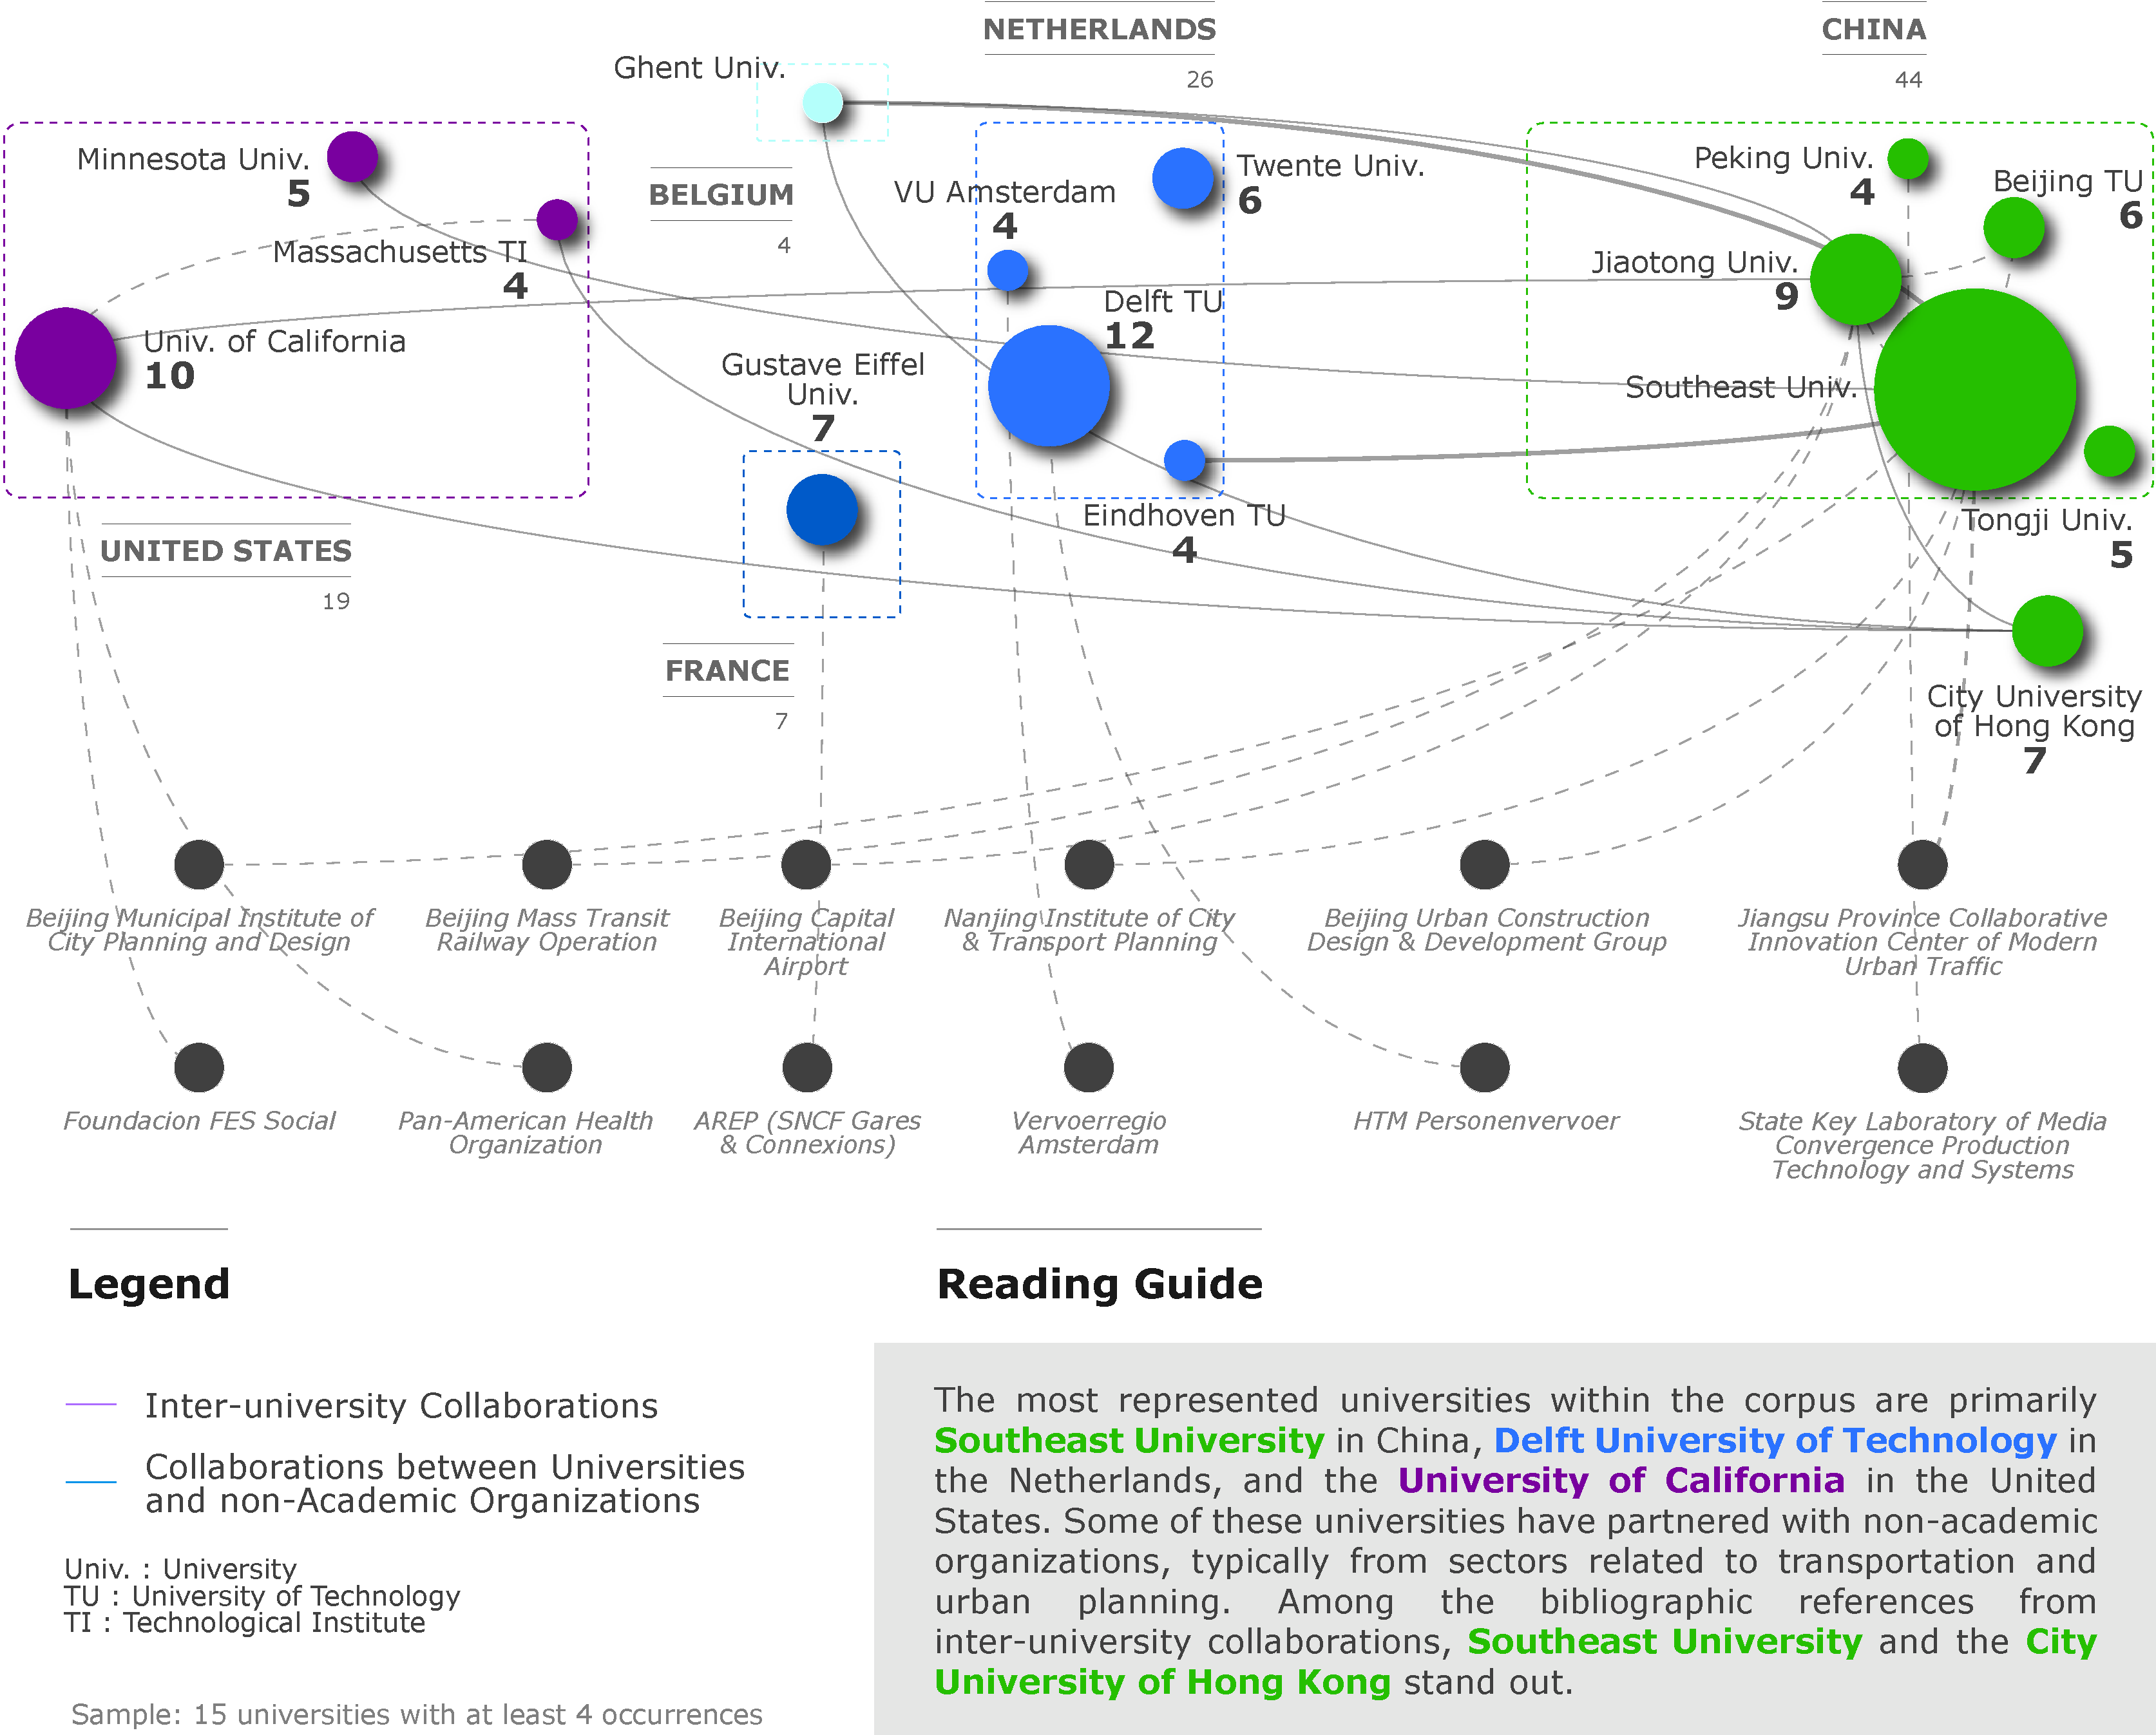
\includegraphics[width=1\columnwidth]{src/Figures/Chap-2/EN_RSL_Collaborations_universites.pdf}}
    \vspace{5pt}
    \begin{flushright}\scriptsize{
    Author: \textcolor{blue}{Dylan Moinse (2023)}
    %\\
    %Created with \Marque{Excel}~and \Marque{Illustrator}
    }\end{flushright}
\end{figure}

    % Universities and Institutions
From the perspective of the institutions represented in the 238 scientific contributions incorporated within the \acrshort{SLR}, a total of 268 unique universities, institutes, organizations, and public or private companies emerge. The fifteen most recurrent institutions represent more than a quarter of the distribution (429 observed values). As shown in \hyperref[fig-chap2:copublications-universites-rsl]{Figure~\ref{fig-chap2:copublications-universites-rsl}} (page~\pageref{fig-chap2:copublications-universites-rsl}), the main universities identified in the documentation are Southeast University in Nanjing (20), followed by Delft University of Technology (12), the University of California, Berkeley (10), Beijing Jiaotong University (9), The Hong Kong Polytechnic University (7), Université Gustave Eiffel in France (7), Beijing University of Technology (6), University of Twente in Enschede (6), Tongji University in Shanghai (5), University of Minnesota Twin Cities in Minneapolis and Saint-Paul (5), Vrije Universiteit Amsterdam (4), Eindhoven University of Technology (4), Ghent University (4), Massachusetts Institute of Technology in Cambridge (4), and finally Peking University (4). %%Translated%%

    % University and Institution Collaborations
By examining scientific collaborations at the university level, it turns out that 128 scientific works are marked by the intersection of at least two academic institutions or research institutes within the same publication. Thus, more than half of the scientific contributions recorded are marked by multi-university co-publications, often spanning distinct continents. The prominent connections observed are concentrated between China, the United States, France, the Netherlands, and Belgium. Among the partnerships that led to such publications, we cite the joint work of Southeast University with Eindhoven University of Technology \textcolor{blue}{\autocite[]{gan_associations_2021, liu_use_2020, liu_understanding_2020}}\index{Gan, Zuoxian|pagebf}\index{Yang, Min|pagebf}\index{Zeng, Qingcheng|pagebf}\index{Timmermans, Harry~J.~P.|pagebf}\index{Liu, Yang|pagebf}\index{Feng, Tao|pagebf}\index{Ji, Yanjie|pagebf}\index{Shi, Zhuangbin|pagebf}\index{Ji, Yanjie|pagebf}\index{Feng, Tao|pagebf}\index{Timmermans, Harry~J.~P.|pagebf} and with Ghent University \textcolor{blue}{\autocite[]{chen_what_2022, cheng_comparison_2023, cheng_exploring_2022}}\index{Chen, Wendong|pagebf}\index{Chen, Xuewu|pagebf}\index{Chen, Jingxu|pagebf}\index{Cheng, Long|pagebf}\index{Huang, Jie|pagebf}\index{Jin, Tanhua|pagebf}\index{Chen, Wendong|pagebf}\index{Li, Aoyong|pagebf}\index{Witlox, Frank|pagebf}\index{Cheng, Long|pagebf}\index{Wang, Kailai|pagebf}\index{Vos, Jonas de|pagebf}\index{Huang, Jie|pagebf}\index{Witlox, Frank|pagebf}, as well as Hong Kong Polytechnic University with the University of California \textcolor{blue}{\autocite{wu_optimal_2020}}\index{Wu, Liyu|pagebf}\index{Gu, Weihua|pagebf}\index{Fan, Wenbo|pagebf}\index{Cassidy, Michael~J.|pagebf} and the Massachusetts Institute of Technology \textcolor{blue}{\autocite{cao_e-scooter_2021}}\index{Cao, Zhejing|pagebf}\index{Zhang, Xiaohu|pagebf}\index{Chua, Kelman|pagebf}\index{Yu, Honghai|pagebf}\index{Zhao, Jinhua|pagebf}. Operational stakeholders are also present in \acrshort{M-TOD} research, primarily in the transport management sector, with joint publications between Jiaotong University and the public transport operator \textsl{Beijing Mass Transit Railway Operation Corporation Limited} \textcolor{blue}{\autocite{wang_interchange_2016}}\index{Wang, Zi-jia|pagebf}\index{Chen, Feng|pagebf}\index{Xu, Tian-kun|pagebf} and \textsl{Beijing Capital International Airport} \textcolor{blue}{\autocite{fan_how_2019}}\index{Fan, Aihua|pagebf}\index{Chen, Xumei|pagebf}\index{Wan, Tao|pagebf}. Similarly, Southeast University forges links with urban actors such as the \textsl{Nanjing Institute of City \& Transport Planning Co.} \textcolor{blue}{\autocite{zhong_layout_2021}}\index{Zhong, Hongming|pagebf}\index{Liu, Zijian|pagebf}\index{Chen, Jun|pagebf}\index{Hao, Jun|pagebf}\index{Wang, Wei|pagebf} and \textsl{Beijing Urban Construction Design \& Development Group Co., Limited} \textcolor{blue}{\autocite{yang_empirical_2016}}\index{Yang, Min|pagebf}\index{Liu, Xinlu|pagebf}\index{Wang, Wei|pagebf}\index{Li, Zhibin|pagebf}\index{Zhao, Jingyao|pagebf}. Furthermore, connections are forming between the University of California and the non-profit organization \acrfull{FES} and the public health organization \textsl{Pan American Health Organization} \textcolor{blue}{\autocite{cervero_influences_2009}}\index{Cervero, Robert|pagebf}\index{Sarmiento, Olga~L.|pagebf}\index{Jacoby, Enrique|pagebf}\index{Gomez, Luis Fernando|pagebf}\index{Neiman, Andrea|pagebf}.%%Translated%%

    % Transition
The bibliometric analysis of the academic corpus focused on a large body of literature, mainly composed of peer-reviewed scientific articles published in English. The analysis framework of the \acrshort{SLR}, based in this first subsection on the contours of research related to \acrshort{M-TOD}, provided an overview of the figures, academic institutions, and scientific journals most influential in this field of study. In the following subsection, we propose to explore the current state of the scientific literature dedicated to \acrshort{TOD} revisited by individual light mobility by conducting a textual analysis of the scientific contributions.%%Translated%%

    % 2.2.1.2. Keywords, Content/Body of the Text
    \needspace{1\baselineskip} % Reserve space
\subsubsection*{Textual Analysis of Academic Publications
    \label{chap2:analyse-textuelle}
    }

    % Introduction
The investigation of the metadata extracted from the academic corpus is, in a second step, based on the lexical systems employed within the research works. This part of the \acrshort{SLR}, intrinsically linked to the textual analysis of academic publications on \acrshort{M-TOD}, aims to identify research practices manifested through the vocabulary used. Initially, the study was differentiated by the language of publication, with the first category being in English, comprising 228 documents, and a second in French, consisting of 10 works. However, due to the low representativity of the French-language works, the textual analysis focuses exclusively on the English-language publications.%%Translated%%

    % Keyword Analysis: Sample and Methodology
Symbolically, the textual examination focused on the content of the research works included in the \acrshort{SLR}, by examining the semantic architecture of the written works, constructed based on the selection of keywords that typically appear after the title and abstract. The aggregation of the academic contributions resulted in the compilation of 1,336 keywords from 208 works, 201 of which are in English. The exploration of the keyword lists defined by the researchers involved in \acrshort{M-TOD} reveals an average of 6.7 keywords per document, considering over 303 distinct terms, of which 260 are in English. To conduct a comparative analysis of the keywords mentioned in the corpus, a preliminary data cleaning phase was undertaken. This process of terminological harmonization involved standardizing keyword sets that share a common origin or related meaning\footnote{~
    For example, the aggregation of the words \Commas{bicyclette}~and \Commas{vélo} in French, or the expressions \Commas{\textsl{transit}}~and \Commas{\textsl{public transport}}, or \Commas{\textsl{subway}}~and \Commas{\textsl{metro}} in English. Although this step is crucial for improving the relevance of the textual data used, it is important to note the assumptions inherent in this work of evaluation.
}.%%Translated%%

    % Keywords: result 1
By cross-referencing the 1,281 English keywords, the textual analysis of this \acrshort{SLR} highlights eleven thematic aspects that stand out within the lexical labels extracted. To conduct this lexical analysis, we first established several thematic categories. Each word was arbitrarily classified according to the category corresponding to its usage context. A graphical highlight of \hyperref[fig-chap2:nuage-mots-cles-rsl]{Figure~\ref{fig-chap2:nuage-mots-cles-rsl}} (page~\pageref{fig-chap2:nuage-mots-cles-rsl}) reveals the clusters of keywords, within which themes related to individual and collective mobility occupy a dominant position. Thus, the concepts related to \Commas{individual modes of transport} (282 occurrences), \Commas{intermodality} (224 occurrences), \Commas{public transport} (202 occurrences), and \Commas{mobility} (181 occurrences) represent the main categories of the ranking, in line with the expression configuration used for the bibliographic search of the \Commas{Corpus EN and FR}, which specifically led to the emergence of these themes (for reference, see \hyperref[table-chap2:expression-recherche-rsl]{Table~\ref{table-chap2:expression-recherche-rsl}}, page~\pageref{table-chap2:expression-recherche-rsl}).%%Translated%%

    % Figure Keyword Cloud RSL
    \begin{figure}[h!]\vspace*{4pt}
        \caption{English keyword clouds extracted from the systematic literature review and classified by theme.}
        \label{fig-chap2:nuage-mots-cles-rsl}
        \centerline{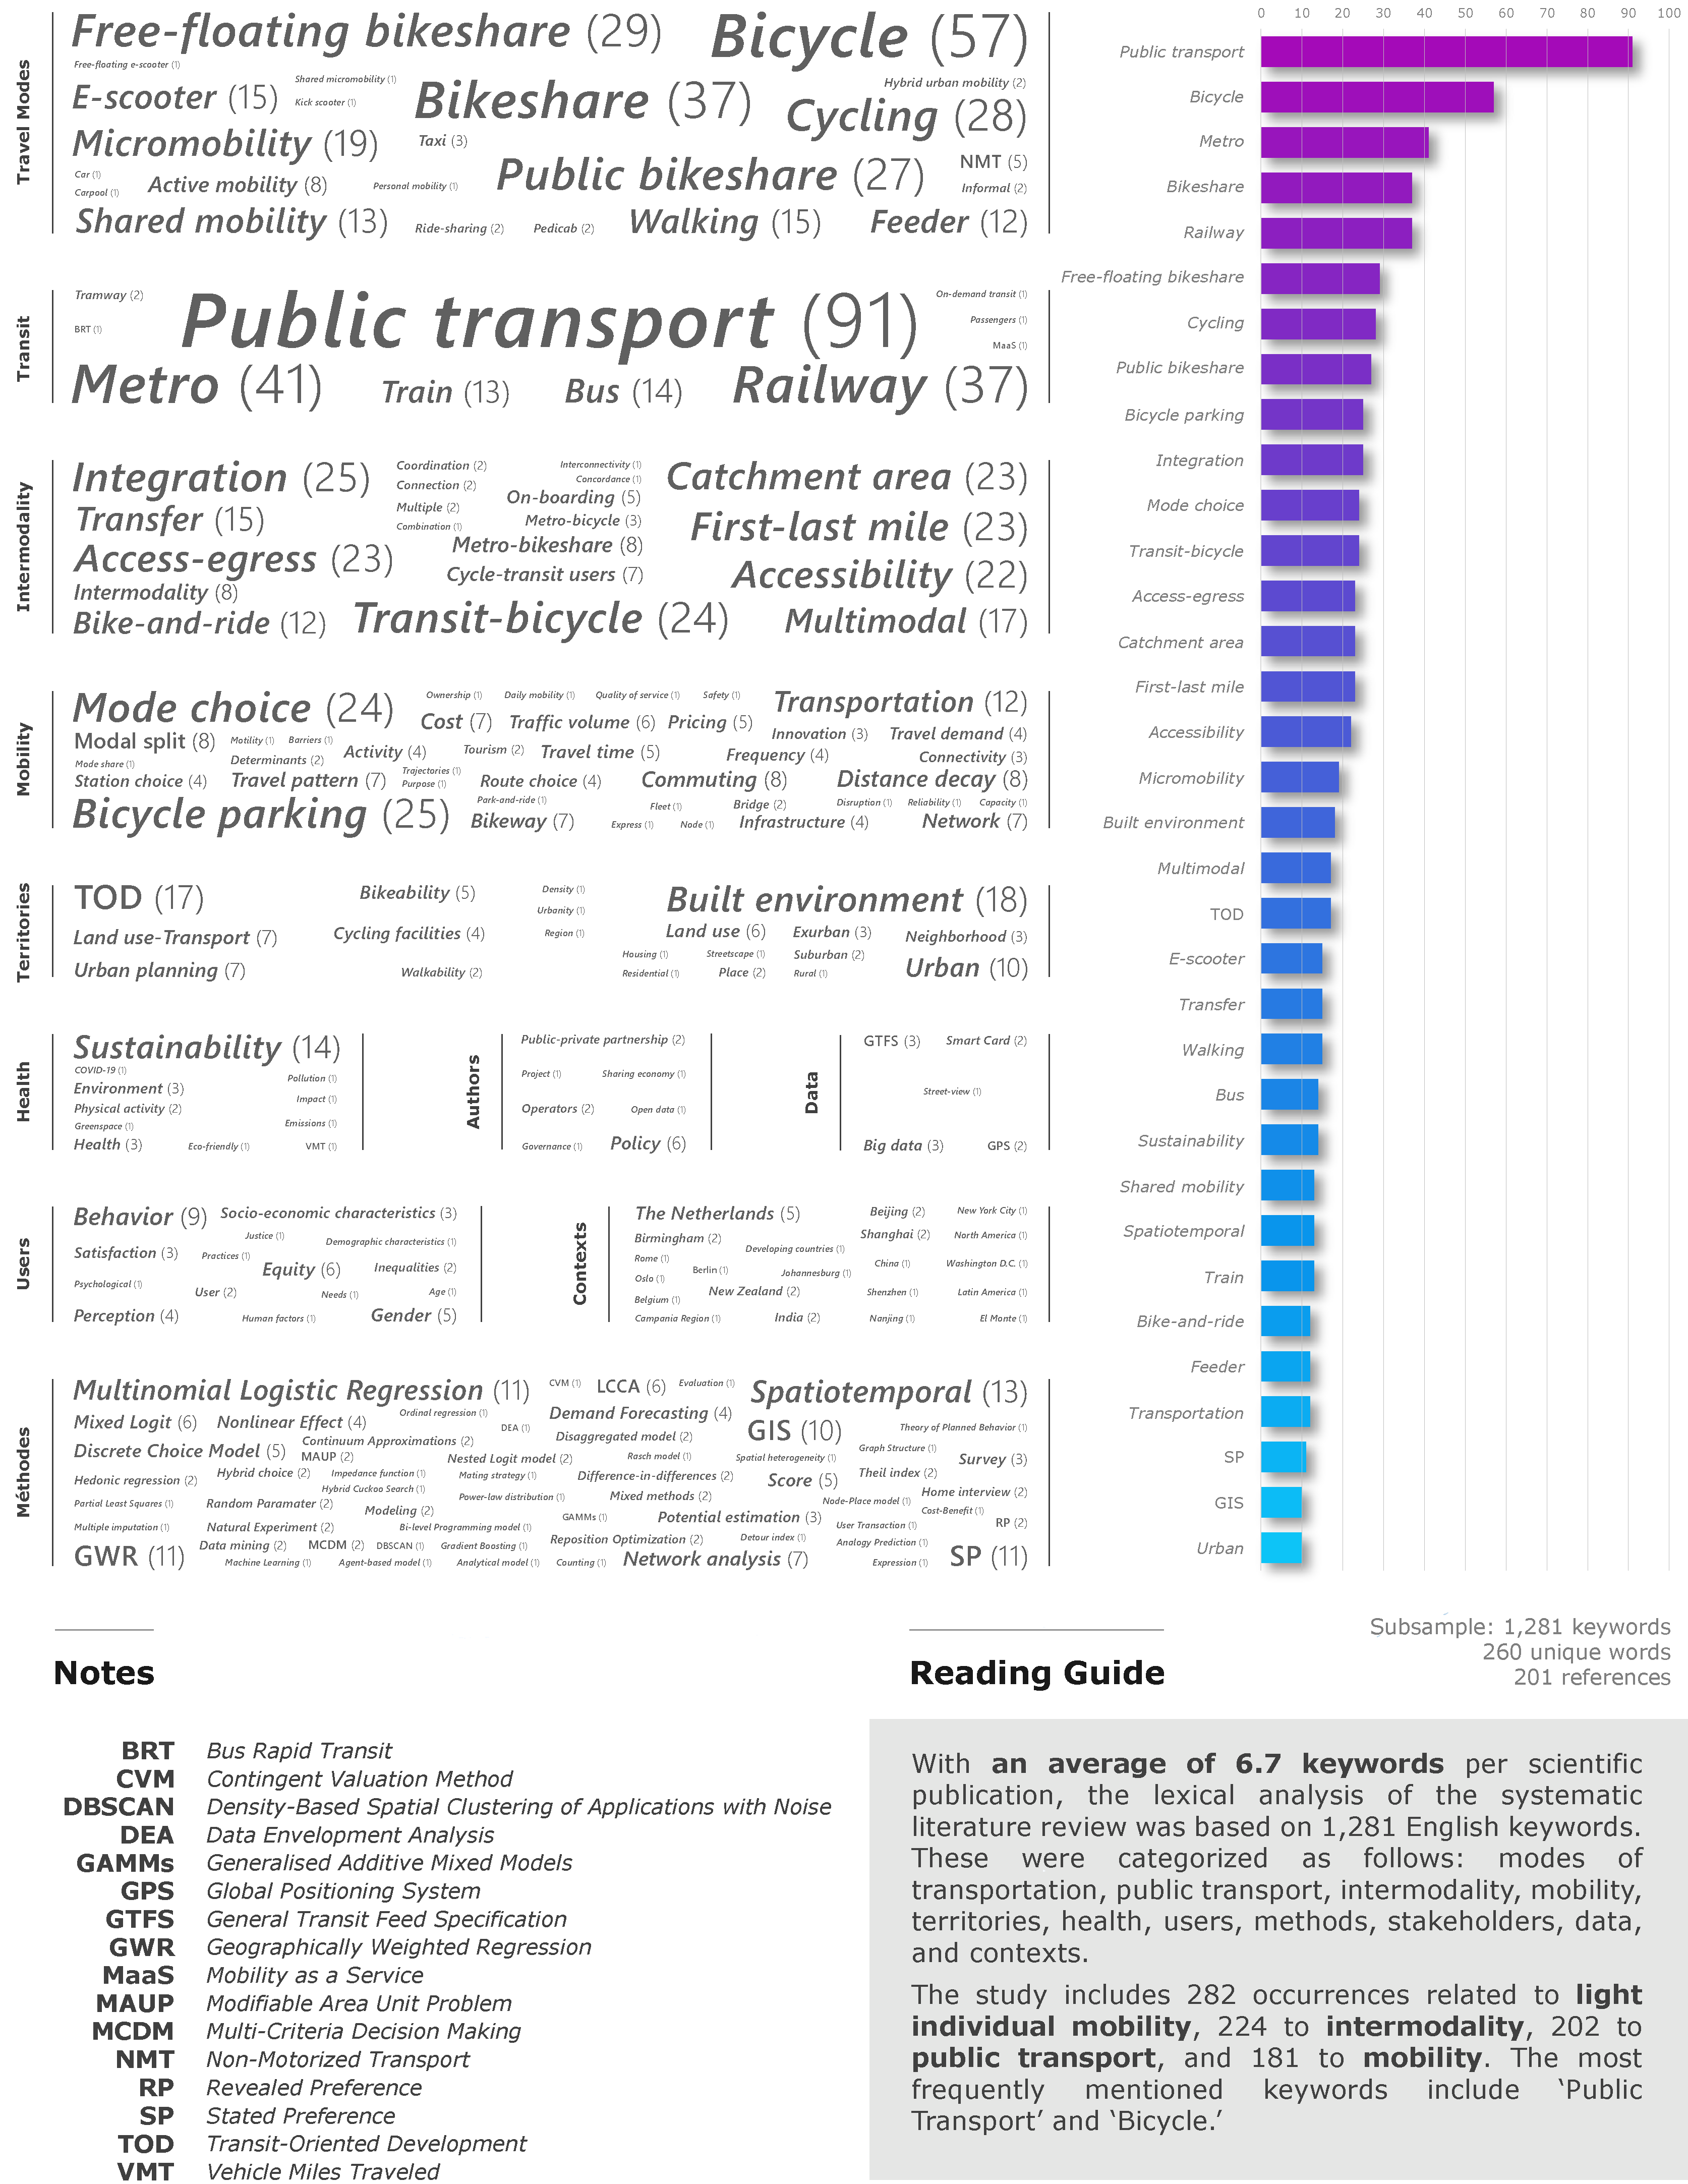
\includegraphics[width=1\columnwidth]{src/Figures/Chap-2/EN_RSL_Nuage_mots_cles_thematiques.pdf}}
        \vspace{5pt}
        \begin{flushright}\scriptsize{
        Author: \textcolor{blue}{Dylan Moinse (2023)}
        %\\
        %Created with \Marque{Python}~and \Marque{Illustrator}
        }\end{flushright}
    \end{figure}

    % Keywords: result 2
At the level of the keywords, it is primarily in the fields of \Commas{public transport} and \Commas{bicycle} that prominent occurrences are found, counting respectively 91 and 57 iterations of terms associated with them. However, this predominance of keywords masks an unequal distribution within each observed theme. While the frequency of keywords related to \Commas{public transport}, \Commas{individual modes of transport}, and \Commas{intermodality} is significant, averaging 20, 12, and 11 occurrences per term, this intensity diminishes to 5.5 and 2 repetitions regarding the categories related to \Commas{mobility}, \Commas{urban planning}, and \Commas{methods}. This observation reflects a broader variety of keywords in these latter themes, alongside a process of terminological homogenization noticeable within the domains of personal transport modes, public transport, and intermodality.%%Translated%%

    % Keywords: result 3
The manipulation of keywords from the perspective of transport modes and infrastructures as objects, such as \Commas{\textsl{bicycle}} (mentioned 57 times), \Commas{\textsl{dockless bikeshare}} (29 occurrences), \Commas{\textsl{public bikeshare}} (27 occurrences), \Commas{\textsl{metro}} (41 occurrences), \Commas{\textsl{railway}} (37 occurrences), and \Commas{\textsl{bicycle parking}} (25 occurrences), reflects an interconnection that crystallizes into lexical signals, perpetuating the conventional pattern in the transport domain (see \hyperref[fig-chap2:nuage-mots-cles-rsl]{Figure~\ref{fig-chap2:nuage-mots-cles-rsl}}, page~\pageref{fig-chap2:nuage-mots-cles-rsl}). Analogous to this approach grounded in the transport paradigm, a vast semantic domain related to the \Commas{turning point of mobility} \textcolor{blue}{\autocites{sheller_new_2006}[8]{sheller_mobilizing_2016}[13]{randell_no_2020}}\index{Sheller, Mimi|pagebf}\index{Urry, John|pagebf}\index{Randell, Richard|pagebf}, is marked by the use of expressions such as \Commas{\textsl{accessibility}} (22 occurrences), \Commas{\textsl{sustainability}} (14 occurrences), \Commas{\textsl{behavior}} (9 occurrences), \Commas{\textsl{policy}} (6 occurrences), \Commas{\textsl{equity}} (6 occurrences), and \Commas{\textsl{bikeability}} (5 occurrences). Indeed, to a lesser extent, we can discern the involvement of urban planning and particularly its connection with mobility, as evidenced by the concept of \Commas{\textsl{TOD}} (17 occurrences) or \Commas{\textsl{land use-transport}} (7 occurrences).%%Translated%%

    % Keywords: result 4
By probing the interactions between the aforementioned keywords, it is interesting to note the close links that associate certain categories with each other. The majority of the word lists tend to establish connections between the categories of \Commas{public transport} and \Commas{individual modes of transport}. Among the 201 English references, 155 of them create a dialogue between these two themes, expressed by the deliberate choice of a list of keywords related to collective and personal mobility. Furthermore, 59 scientific publications stand out for their specific configuration, forming an ordered lexical sequence as follows: the first keyword in the list refers to \Commas{public transport}, followed by \Commas{individual modes of transport}, and a third term invoking \Commas{intermodality}.%%Translated%%

    % Figure Keywords content RSL
    \begin{figure}[h!]\vspace*{4pt}
        \caption{Keyword cloud from the full content of the English-language academic works included in the systematic literature review.}
        \label{fig-chap2:contenu-textuel-rsl}
        \centerline{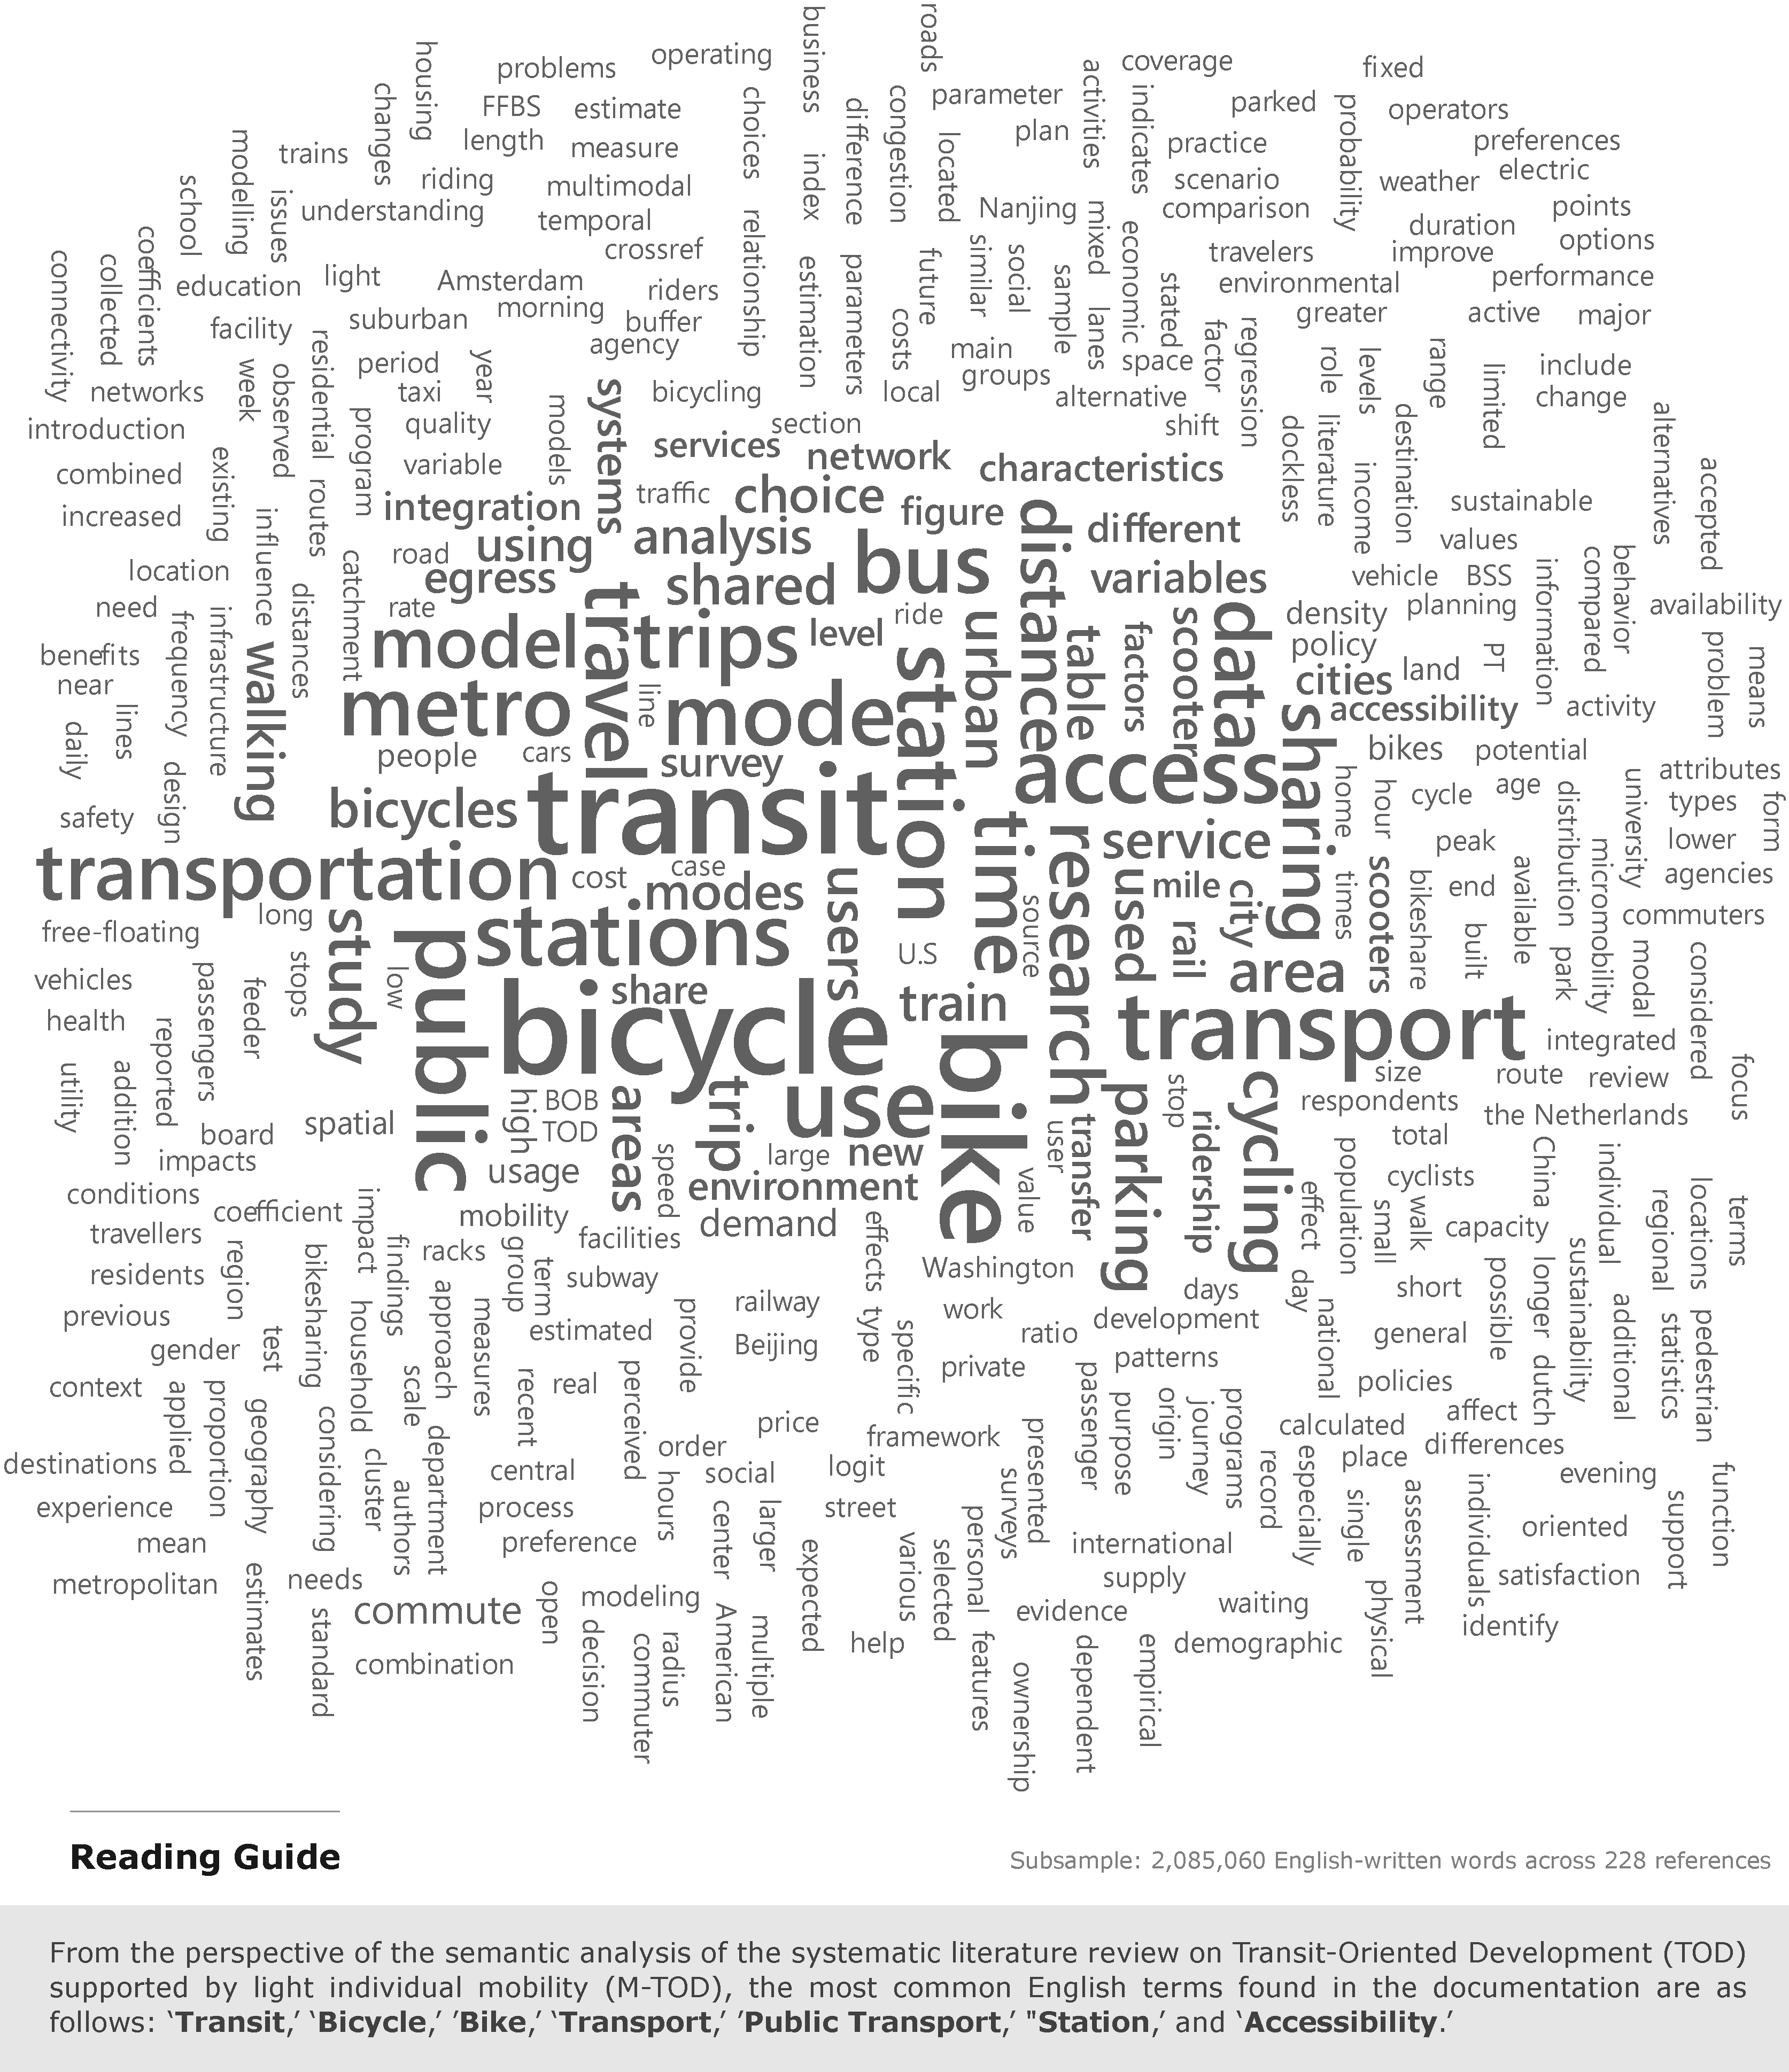
\includegraphics[width=1\columnwidth]{src/Figures/Chap-2/EN_RSL_Mots_contenu.pdf}}
        \vspace{5pt}
        \begin{flushright}\scriptsize{
        Author: \textcolor{blue}{Dylan Moinse (2023)}
        %\\
        %Created with \Marque{Python}~and \Marque{Illustrator}
        }\end{flushright}
    \end{figure}

    % RSL Word Content
The textual analysis was deepened through an examination of the full content of each English-language scientific publication. As shown in \hyperref[fig-chap2:contenu-textuel-rsl]{Figure~\ref{fig-chap2:contenu-textuel-rsl}} (page~\pageref{fig-chap2:contenu-textuel-rsl}), the examination of the hundred most recurrent terms within the documents\footnote{~
    In order to classify the lexical fields identified in the analyzed documents, we first performed a cleaning step by excluding terms related to everyday life or general scientific research in the English language. These common expressions were later excluded from the analysis, such as \Commas{\textsl{the}}, \Commas{\textsl{a}}, \Commas{\textsl{and}}, \Commas{\textsl{we}}, \Commas{\textsl{for}}, \Commas{\textsl{study}}, \Commas{\textsl{scientific}}, \Commas{\textsl{methods}} and \Commas{\textsl{results}}.
} reinforces the trend previously identified at the keyword level, primarily marked by the predominance of terms such as \Commas{\textsl{transit}}, \Commas{\textsl{bicycle}}, \Commas{\textsl{bike}}, \Commas{\textsl{transport}}, \Commas{\textsl{public transport}}, \Commas{\textsl{station}}, and \Commas{\textsl{accessibility}}. However, it is important to highlight the substantial influence of some terms, such as \Commas{\textsl{use}}, \Commas{\textsl{access}}, \Commas{\textsl{distance}}, \Commas{\textsl{area}}, \Commas{\textsl{users}}, or \Commas{\textsl{service}}, which are related to usage, users, and distances or travel times. On the other hand, it should be noted that the lexical presence related to urban planning remains practically absent in the writings, except for a few event-driven occurrences, such as \Commas{\textsl{density}}, \Commas{\textsl{mixed}}, \Commas{\textsl{TOD}}, or \Commas{\textsl{land}}.%%Translated%%

    % Transition
Upon reviewing the terms scrutinized within the \acrshort{SLR} corpus, the various collective and individual transport modes, central to a transit-oriented urban development supported by individual light mobility, emerge as the foremost themes. Given the rapid evolution of mobility practices, technologies, and techniques pertaining to these different transportation modes, the following subsection aims to contextualize research works related to the \acrshort{M-TOD}, focusing on the development of emerging areas of investigation.%%Translated%%

    % 2.2.1.3. micromobility, TC
    \needspace{1\baselineskip} % Space reservation
\subsubsection*{Evolution of Research on the Synergy between Public Transport and Light Individual Mobility
    \label{chap2:evolution-recherches-tc-mobilite-individuelle-legere}
    }

    % Trend Since 1993
The analysis of the temporal distribution of the scientific publications included in the \acrshort{SLR} offers a comprehensive perspective on the characteristics and advancements that delimit this body of literature. The chronological trajectory of the bibliographic corpus dedicated to the integration of light individual mobility into public transport networks depicts continuous growth between 1993 and 2021. From 2015 onward, the annual threshold of ten scientific publications was consistently exceeded, suggesting growing research interest in this topic. In just four consecutive years, the number of academic papers doubled, with 129 new works published between 2019 and the beginning of 2023.%%Translated%%

    % Objective
In line with the methodological protocol defined in this \acrshort{SLR}, the minimum date for this bibliometric study was set to 1993, referencing the conceptualization of \acrshort{TOD} by \textcolor{blue}{Peter} \textcolor{blue}{\textcite{calthorpe_next_1993}}\index{Calthorpe, Peter|pagebf}. The bibliographic study presented here aims to reveal the characteristics of this corpus developed over three decades of international research. However, it is essential to acknowledge the existence of earlier works addressing the subject of study. While the observed growth of scientific publications includes works in both English and French, the emergence of French-language works occurred at a later stage, starting in 2015. However, this subset remains small, making it difficult to draw definitive conclusions. On the other hand, the scientific literature in European contexts began to develop early, as early as 2000.%%Translated%%

    % Figure Chronology RSL Transport Modes
    \begin{figure}[h!]\vspace*{4pt}
        \caption{Evolution of scientific publications on the combination of public transport and light individual mobility within the systematic literature review.}
        \label{fig-chap2:chronologie-modes-deplacements-rsl}
        \centerline{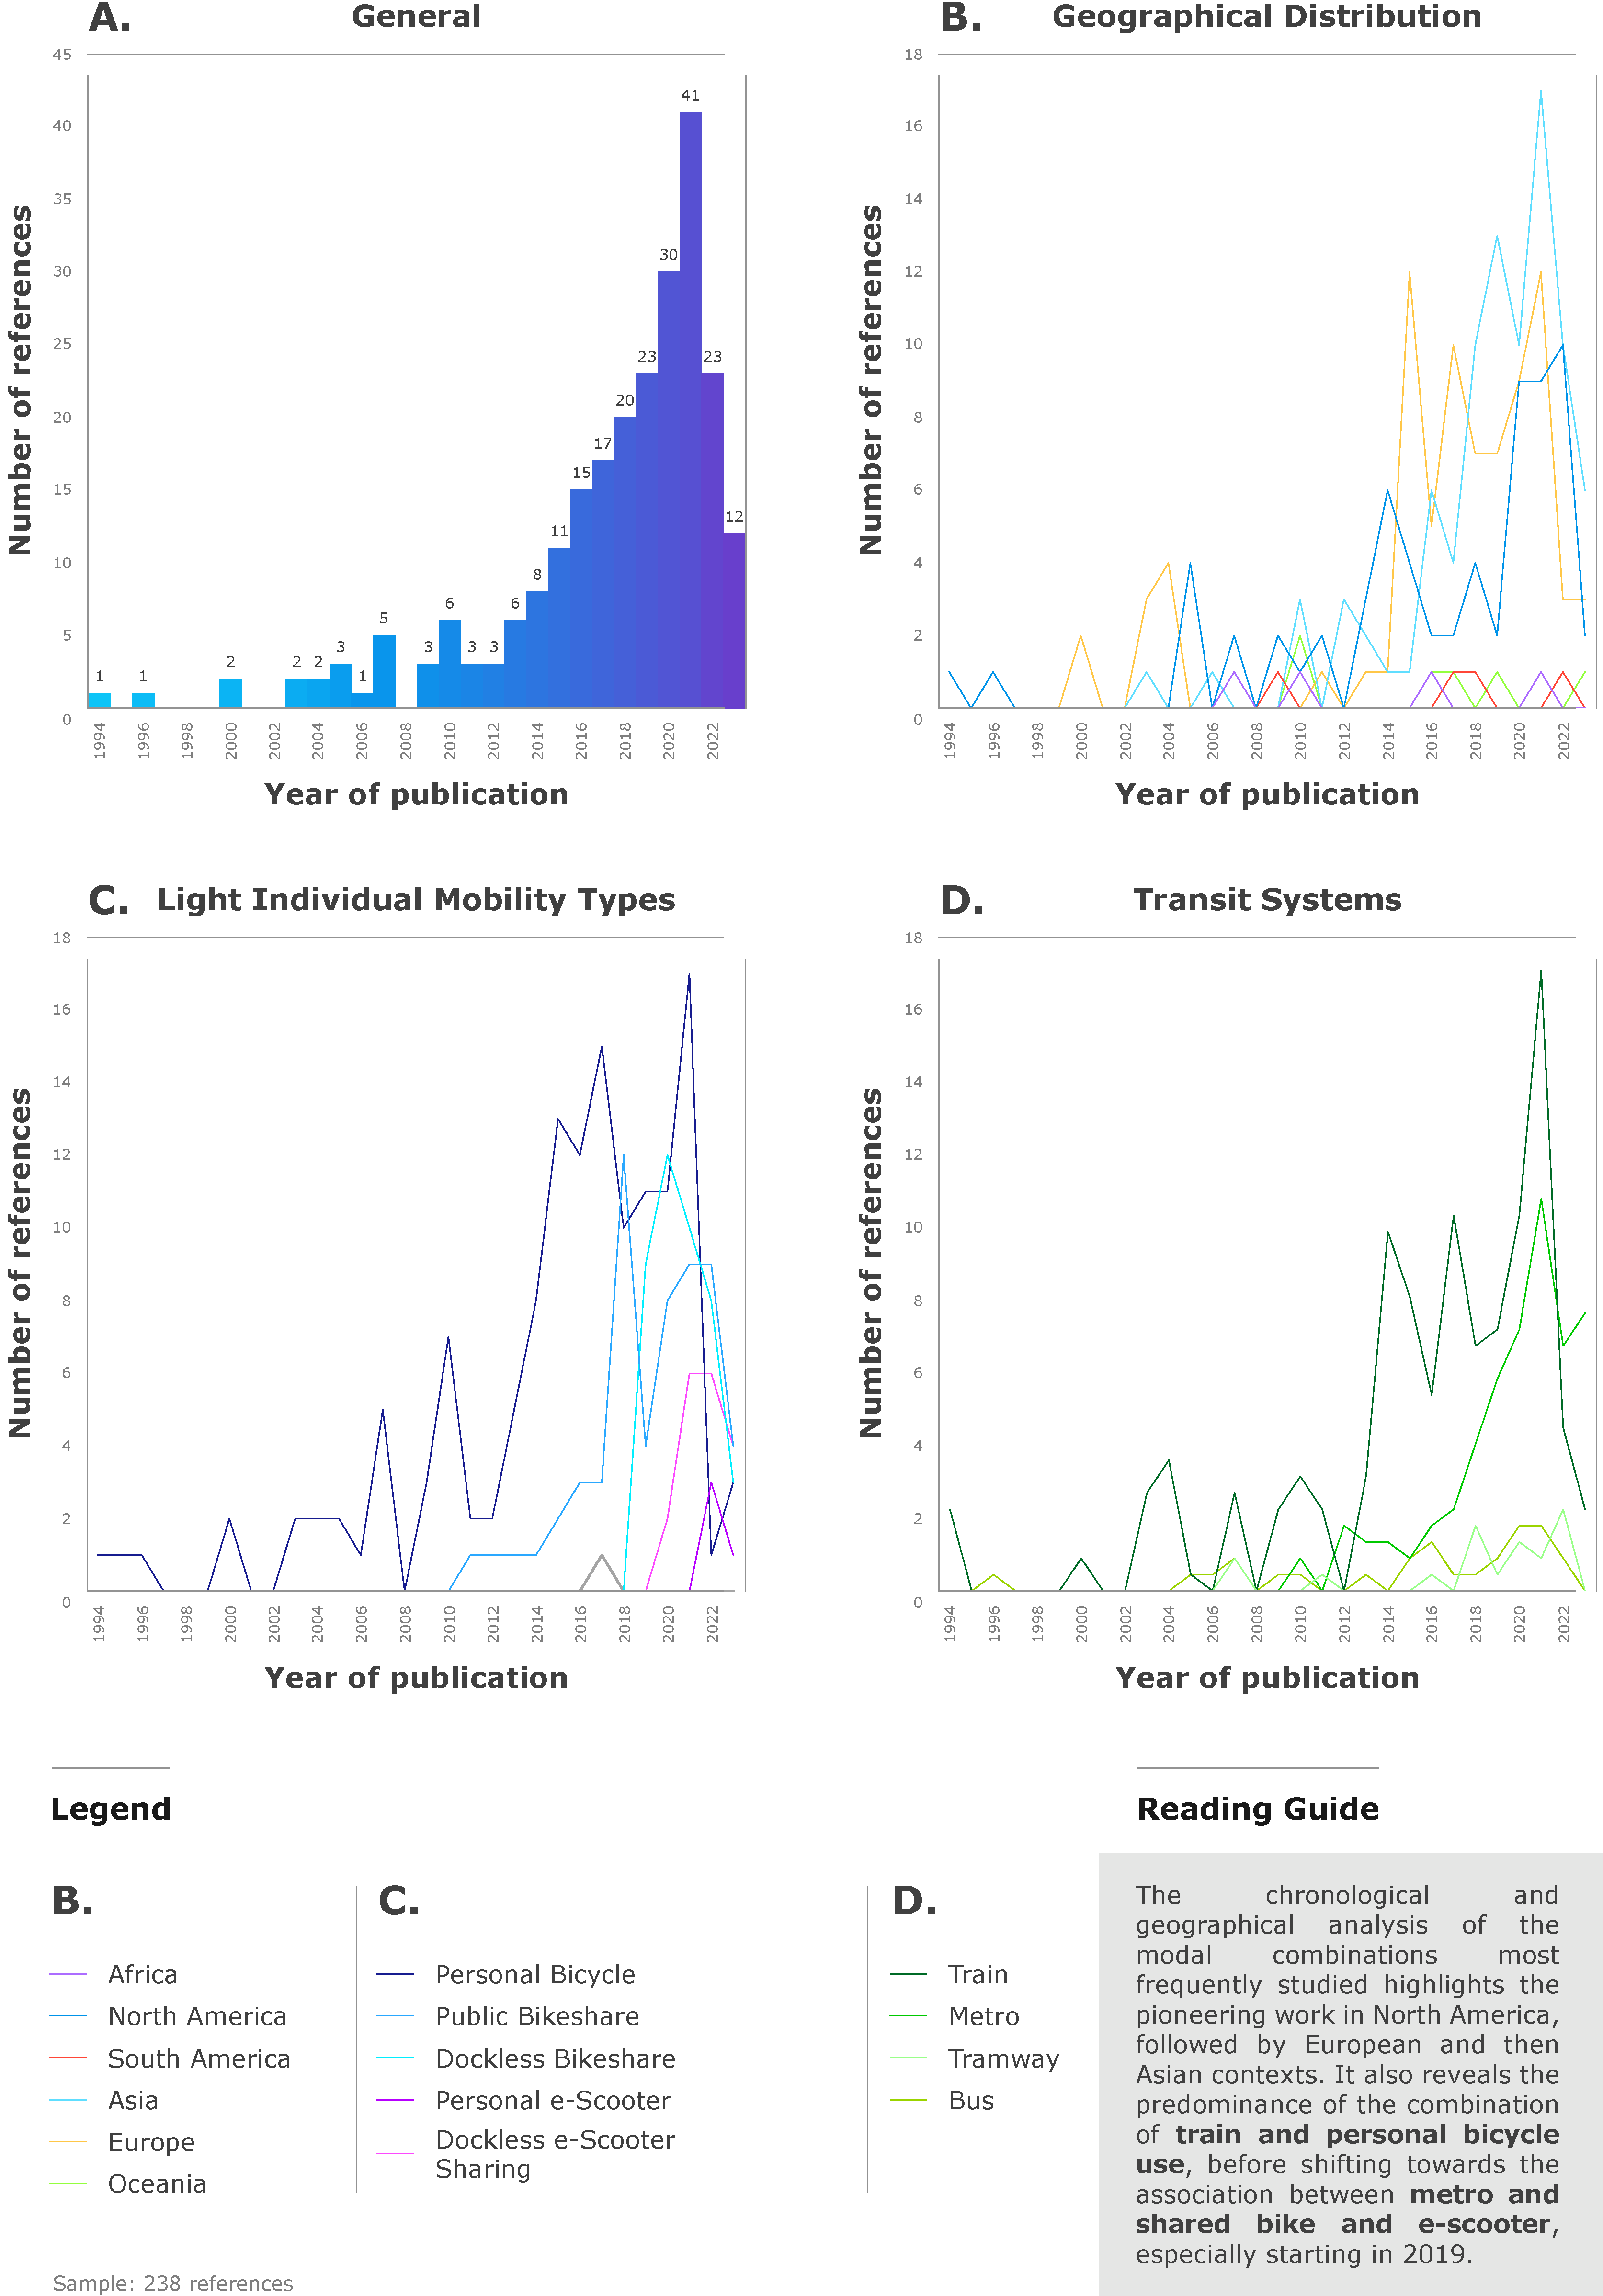
\includegraphics[width=1\columnwidth]{src/Figures/Chap-2/EN_RSL_Chronologie.pdf}}
        \vspace{5pt}
        \begin{flushright}\scriptsize{
        Author: \textcolor{blue}{Dylan Moinse (2023)}
        %\\
        %Created with \Marque{Excel}, \Marque{Python}, and \Marque{Illustrator}
        }\end{flushright}
    \end{figure}

    % Chronology by Micromobility
The chronological approach to \acrshort{M-TOD}, as depicted in the scientific literature, offers insightful perspectives on the rise of light individual mobility (see \hyperref[annexes:rsl-combinaisons-modales]{Appendix~\ref{annexes:rsl-combinaisons-modales}}, page~\pageref{annexes:rsl-combinaisons-modales}) and its potential contribution to the development of the urban model. \hyperref[fig-chap2:chronologie-modes-deplacements-rsl]{Figure~\ref{fig-chap2:chronologie-modes-deplacements-rsl}} (page~\pageref{fig-chap2:chronologie-modes-deplacements-rsl}) reveals the prominent role that conventional bicycles held in international research from 1994 to 2017, representing 89\% of the publications during that period. However, this dominant position has gradually been challenged, with the traditional bicycle being present in only 41\% of studies between 2018 and 2021, and in just 4\% of the most recent publications. This unfavorable trend initially benefited the exploration of \acrfull{PBS}, which saw increased interest starting in 2011. Later, from 2019 onwards, attention shifted to \acrfull{DBS}. More recently, the research corpus has shown a growing interest in \acrfull{DESS}. However, \acrfull{PeS} remains absent from the studies, highlighting a stark contrast between the recent boom in research on shared mobility services and the scarcity of studies on private electric scooter use. This observation should be understood within the context of the rise of shared bicycles and micromobility, as evidenced by the descriptive analysis conducted by \textcolor{blue}{\textcite[298]{zhang_built_2023}}\index{Zhang, Yushan|pagebf}\index{Kasraian, Dena|pagebf}\index{Wesemael, Pieter van|pagebf} in their \acrshort{SLR}, which shows that three-quarters of the documentation on this subject emerged between 2019 and 2022.%%Translated%%

    % Chronology by Public Transport
The sequential study of public transport systems examined in the scientific literature also sheds light on the general trends that have emerged over the three decades under investigation. As indicated in \hyperref[fig-chap2:chronologie-modes-deplacements-rsl]{Figure~\ref{fig-chap2:chronologie-modes-deplacements-rsl}} (page~\pageref{fig-chap2:chronologie-modes-deplacements-rsl}), international research on \acrshort{M-TOD} showed particular interest in intercity rail modes from 1994 to 2017, with particular focus on \acrfull{TER}, in conjunction with the conventional bicycle. In contrast, the metro system, which had been relatively overlooked until 2012, saw a resurgence of interest from 2019, coinciding with the increased focus on \acrshort{DBS} and \acrshort{DESS} systems. Furthermore, studies on the integration of light individual mobility with buses, particularly \acrfull{BRT}, as well as with trams, maintain a secondary but consistent presence in the scientific publications. Overall, the chronological analysis of the most frequently studied modal combinations reveals a main pattern: the initial dominance of the train and personal bicycle pairing in academic works on \acrshort{M-TOD}, gradually giving way to the combination of metro and bike and micromobility services.%%Translated%%

    % Chronology by Shared Micromobilities (Maturation)
Although the scientific literature on light individual mobility, particularly on shared bicycles and micromobility, has developed in recent years, research focuses on various stages of development of these mobility services in the surveyed territories. By examining the period difference between when the light individual mobility service was launched and when the data was collected and processed in the analyzed documentation, we explored the different maturation stages studied based on the modes of transport involved in bike and scooter sharing. These mobility services are mostly studied during their recent development, about three years (forty months) after being launched in the territory \textcolor{blue}{\autocite[298]{zhang_built_2023}}\index{Zhang, Yushan|pagebf}\index{Kasraian, Dena|pagebf}\index{Wesemael, Pieter van|pagebf}. However, the standard deviation of the observed distribution is quite large, with an average difference of four years, meaning that a significant proportion of research focuses on a more advanced stage of development. This unequal distribution is notably explained by the differences in the type of shared light individual mobility analyzed:
    \begin{customitemize}
        \item The corpus on \acrshort{PBS} systems is the most diverse, with studies mostly focusing on services that have been operational for five years. Notable works by \textcolor{blue}{\textcite{aljeri_impacts_2020, andersson_neighbourhood_2021, ma_estimating_2019, ashraf_impacts_2021, liu_understanding_2020, kuijk_preferences_2022, gu_measuring_2019, kong_deciphering_2020, radzimski_exploring_2021, romm_differences_2022, tarpin-pitre_typology_2020}}\index{Aljeri, Moathe|pagebf}\index{Andersson, David Emanuel|pagebf}\index{Ma, Ting|pagebf}\index{Ashraf, Md Tanvir|pagebf}\index{Liu, Yang|pagebf}\index{Kuijk, Roy~J. van|pagebf}\index{Gu, Tianqi|pagebf}\index{Kong, Hui|pagebf}\index{Radzimski, Adam|pagebf}\index{Dzięcielski, Michał|pagebf}\index{Romm, Daniel|pagebf}\index{Verma, Priyanka|pagebf}\index{Karpinski, Elizabeth|pagebf}\index{Sanders, Tracy~L.|pagebf}\index{McKenzie, Grant|pagebf}\index{Tarpin-Pitre, Léandre|pagebf} focus on the impacts of \acrshort{PBS} on public transport networks in New York City, Taipei, Washington D.C., Nanjing, Suzhou, Boston, and Montreal, between five and seven years after launch. In contrast, \textcolor{blue}{\textcite{cheng_promoting_2022, cheng_expanding_2018, yen_how_2023, tang_uncovering_2021, bocker_bike_2020}}\index{Cheng, Long|pagebf}\index{Jin, Tanhua|pagebf}\index{Wang, Kailai|pagebf}\index{Lee, Yongsung|pagebf}\index{Witlox, Frank|pagebf}\index{Cheng, Yung-Hsiang|pagebf}\index{Yen,~B.T.H.|pagebf}\index{Mulley, Corinne|pagebf}\index{Yeh, Chia-Jung|pagebf}\index{Tang, Jinjun|pagebf}\index{Böcker, Lars|pagebf} analyze the impact of urban environment on mobility systems in Nanjing, Kaohsiung, Taipei, Shenzhen, and Oslo, eight to fifteen years after launch;
        \item \acrshort{DBS} is generally studied two years after its deployment in the territory, while the first quarter of publications on this topic explores the service less than a year after launch. Thus, \textcolor{blue}{\textcite{chen_what_2022, fan_dockless_2020, qiu_interplay_2021, fan_how_2019, jin_competition_2019, li_integration_2020, li_unbalanced_2022, li_factors_2020, liu_use_2020, wu_identification_2023, yang_spatiotemporal_2019}}\index{Chen, Wendong|pagebf}\index{Fan, Yichun|pagebf}\index{Qiu, Waishan|pagebf}\index{Jin, Haitao|pagebf}\index{Jin, Fengjun|pagebf}\index{Wang, Jiao'e|pagebf}\index{Sun, Wei|pagebf}\index{Dong, Libo|pagebf}\index{Li, Jie|pagebf}\index{Li, Lili|pagebf}\index{Li, Xuefeng|pagebf}\index{Liu, Yang|pagebf}\index{Wu, Hao|pagebf}\index{Wang, Yanhui|pagebf}\index{Sun, Yuqing|pagebf}\index{Yin, Duoduo|pagebf}\index{Li, Zhanxing|pagebf}\index{Luo, Xiaoyue|pagebf}\index{Yang, Yuanxuan|pagebf} study the use of \acrshort{DBS} in combination with public transport networks in Nanjing, Beijing, Ithaca, Suzhou, Shenzhen, Nanjing, and Nanchang, one to two years after its introduction. Similarly, as with \acrshort{PBS}, \textcolor{blue}{\textcite{cheng_exploring_2022, chu_last_2021, guo_built_2020, guo_role_2021, hu_study_2019}}\index{Cheng, Long|pagebf}\index{Wang, Kailai|pagebf}\index{Vos, Jonas de|pagebf}\index{Huang, Jie|pagebf}\index{Witlox, Frank|pagebf}\index{Chu, Junhong|pagebf}\index{Duan, Yige|pagebf}\index{Yang, Xianling|pagebf}\index{Wang, Li|pagebf}\index{Guo, Yuanyuan|pagebf}\index{Hu, Li|pagebf}\index{He, Sylvia~Y.|pagebf} focus on the role of the urban environment related to \acrshort{DBS} in intermodality, in Nanjing, Beijing, and Shenzhen;
        \item Lastly, half of the literature on \acrshort{DESS} in combination with public transport adopts a territory benefiting from shared micromobility for less than a year. All the scientific productions on this subject examine the use of \acrshort{DESS} in intermodality, in Seoul, Austin, Rome, Seattle, Oslo, Berlin, New York City, Columbus, Chicago, and Nashville \textcolor{blue}{\autocite{baek_electric_2021, zuniga-garcia_evaluation_2022, vinagre_diaz_blind_2023, beale_integrating_2023, fearnley_patterns_2020, heumann_spatiotemporal_2021, lee_forecasting_2021, li_measuring_2022, mohammadian_analyzing_2022, ziedan_complement_2021}}\index{Baek, Kwangho|pagebf}\index{Zuniga-Garcia, Natalia|pagebf}\index{Vinagre Díaz, Juan José|pagebf}\index{Beale, Kirsten|pagebf}\index{Fearnley, Nils|pagebf}\index{Heumann, Maximilian|pagebf}\index{Li, Mina|pagebf}\index{Li, Xia|pagebf}\index{Mohammadian, Abolfazl|pagebf}\index{Ziedan, Abubakr|pagebf}\index{Shah, Nitesh~R.|pagebf}\index{Wen, Yi|pagebf}\index{Brakewood, Candace|pagebf}\index{Cherry, Christopher~R.|pagebf}\index{Cole, Justin|pagebf}.
    \end{customitemize}%%Translated%%

    % Discussion of Maturation
From this observation, it is clear that bike-sharing and shared micromobility services do not all share the same temporal framework between their implementation and the period of investigation. This statistical analysis highlights implications regarding the preference for certain research themes suited to the temporal context. In general, \acrshort{PBS} systems have had sufficient maturation time to be evaluated for their effects on mobility and urban systems. In contrast, the more recent \textsl{dockless} services benefit more from studies related to mobility behaviors and their regulation in urban environments, while their long-term impacts on territories remain significantly less explored.%%Translated%%

    % Chronology by Geographic Areas and Transition
By deepening the analysis of the evolution of research topics, from the train-and-bike duo to the metro-and-shared mobility services, it is possible to incorporate a new variable related to the geography of the research areas selected. European case studies are abundant when both the temporal dimension of publications and the geographic regions analyzed within the \acrshort{M-TOD} context are considered. From the period 2000 to 2009, bibliographic references associated with a European geographic area account for 8 of the 18 documents dedicated to the \acrshort{SLR}, while from 2010 onwards, only 62 out of the 218 investigations listed refer to a geographic area within the Old Continent. Indeed, research on the interactions between public transport networks and light individual mobility in Europe primarily focuses on the existing or potential relationships between the \acrshort{TER} and the individually used bicycle (see \hyperref[fig-chap2:chronologie-modes-deplacements-rsl]{Figure~\ref{fig-chap2:chronologie-modes-deplacements-rsl}}, page~\pageref{fig-chap2:chronologie-modes-deplacements-rsl}). This transition can be attributed to the emergence of Asian territories from 2010 and the resurgence of North American investigations from 2013 onwards. In the following subsection, which discusses the current state of the scientific literature on a \acrshort{TOD} incorporating light individual mobility, we will report the geographical distribution of scientific publications to understand the temporal and spatial contours of this research topic.%%Translated%%

    % 2.2.1.4. Geographic Areas
    \needspace{1\baselineskip} % Space reservation
\subsubsection*{Exploration of Geographic Areas Covered
    \label{chap2:exploration-terrains-geographiques}
    }

    % Geographic Distribution by Continent
Examining the geographic areas studied in the academic literature provides context to the observed phenomena, while contributing to a holistic understanding of the research issues and identifying certain gaps. The chronological approach adopted in the bibliometric analysis reveals a marked prevalence of the three previously mentioned continents: North America, Asia, and Europe. The \Commas{New Triad,} as the triptych of the main global exchange hubs, accounts for a substantial share of the selected case studies, with 26.4\%, 36\%, and 32\% respectively for the three regions mentioned. In contrast, Africa, South America, and Oceania show a marginal presence in the database, representing only 6\% of the bibliographic record (see \hyperref[fig-chap2:terrains-geographiques-continents]{Map~\ref{fig-chap2:terrains-geographiques-continents}}, page~\pageref{fig-chap2:terrains-geographiques-continents}). Of the 59 scientific articles on bicycles and micromobility in the \acrshort{SLR} published by \textcolor{blue}{\textcite[298]{zhang_built_2023}}\index{Zhang, Yushan|pagebf}\index{Kasraian, Dena|pagebf}\index{Wesemael, Pieter van|pagebf}, 48 of them examine territories in Europe, North America, or Asia.%%Translated%%

    % Map of Geographic Areas by Country
    \begin{carte}[h!]\vspace*{4pt}
        \caption{Map of geographic areas explored in the systematic literature review, aggregated by country.}
        \label{fig-chap2:terrains-geographiques-continents}
        \centerline{\includegraphics[width=1\columnwidth]{src/Figures/Chap-2/EN_RSL_Carte_Monde.pdf}}
        \vspace{5pt}
        \begin{flushleft}\scriptsize{
        \textcolor{blue}{Note:} Only countries with two or more contributions are shown on the map.
        }\end{flushleft}
        \begin{flushright}\scriptsize{
        Author: \textcolor{blue}{Dylan Moinse (2023)}
        }\end{flushright}
    \end{carte}

    % Geographic Distribution by Country
On a finer scale, the countries most represented in the \acrshort{SLR} dedicated to \acrshort{M-TOD} are China and the United States, followed by the Netherlands, in line with the locations of the researchers' activities listed in \hyperref[chap2:analyse-bibliometrique]{Subsection~2.1.1.} (page~\pageref{chap2:analyse-bibliometrique}). Together, these three countries represent 63.6\% of the geographic areas considered in the research works. The remaining third is distributed among a mosaic of countries, some industrialized and others emerging, including France, India, South Korea, Taiwan, Canada, Germany, and Italy (see \hyperref[fig-chap2:terrains-geographiques-continents]{Map~\ref{fig-chap2:terrains-geographiques-continents}}, page~\pageref{fig-chap2:terrains-geographiques-continents}). As a result, it would be more accurate to refer to Western Europe, North America, and East Asia as the geographic regions that clearly prevail in this \acrshort{SLR}. This finding aligns with the literature review produced by \textcolor{blue}{Bárbara} \textcolor{blue}{\textcite[17]{jansson_almeida_alternativas_2022}}\index{Jansson Almeida, Bárbara|pagebf}, on the integration of bicycles with the metro, which highlights the significant presence of studies conducted in China, the Netherlands, and the United States. An analysis of the corpus at the scale of metropolitan areas and cities reveals a concentration around megacities, primarily in Asia and the United States. Globalized regions along the Chinese coast, such as Beijing, Nanjing, Shanghai, and Shenzhen, dominate this ranking. In the United States, major urban hubs such as Washington~D.C., Boston, and New York City also rank highly. In Europe, the focal points shift to regional centers, notably The Hague and Amsterdam (see \hyperref[fig-chap2:terrains-geographiques-villes]{Map~\ref{fig-chap2:terrains-geographiques-villes}}, page~\pageref{fig-chap2:terrains-geographiques-villes}).%%Translated%%

    % Map of Geographic Areas by City
    \begin{carte}[h!]\vspace*{4pt}
        \caption{Geographic distribution of major metropolitan areas examined in the systematic literature review.}
        \label{fig-chap2:terrains-geographiques-villes}
        \centerline{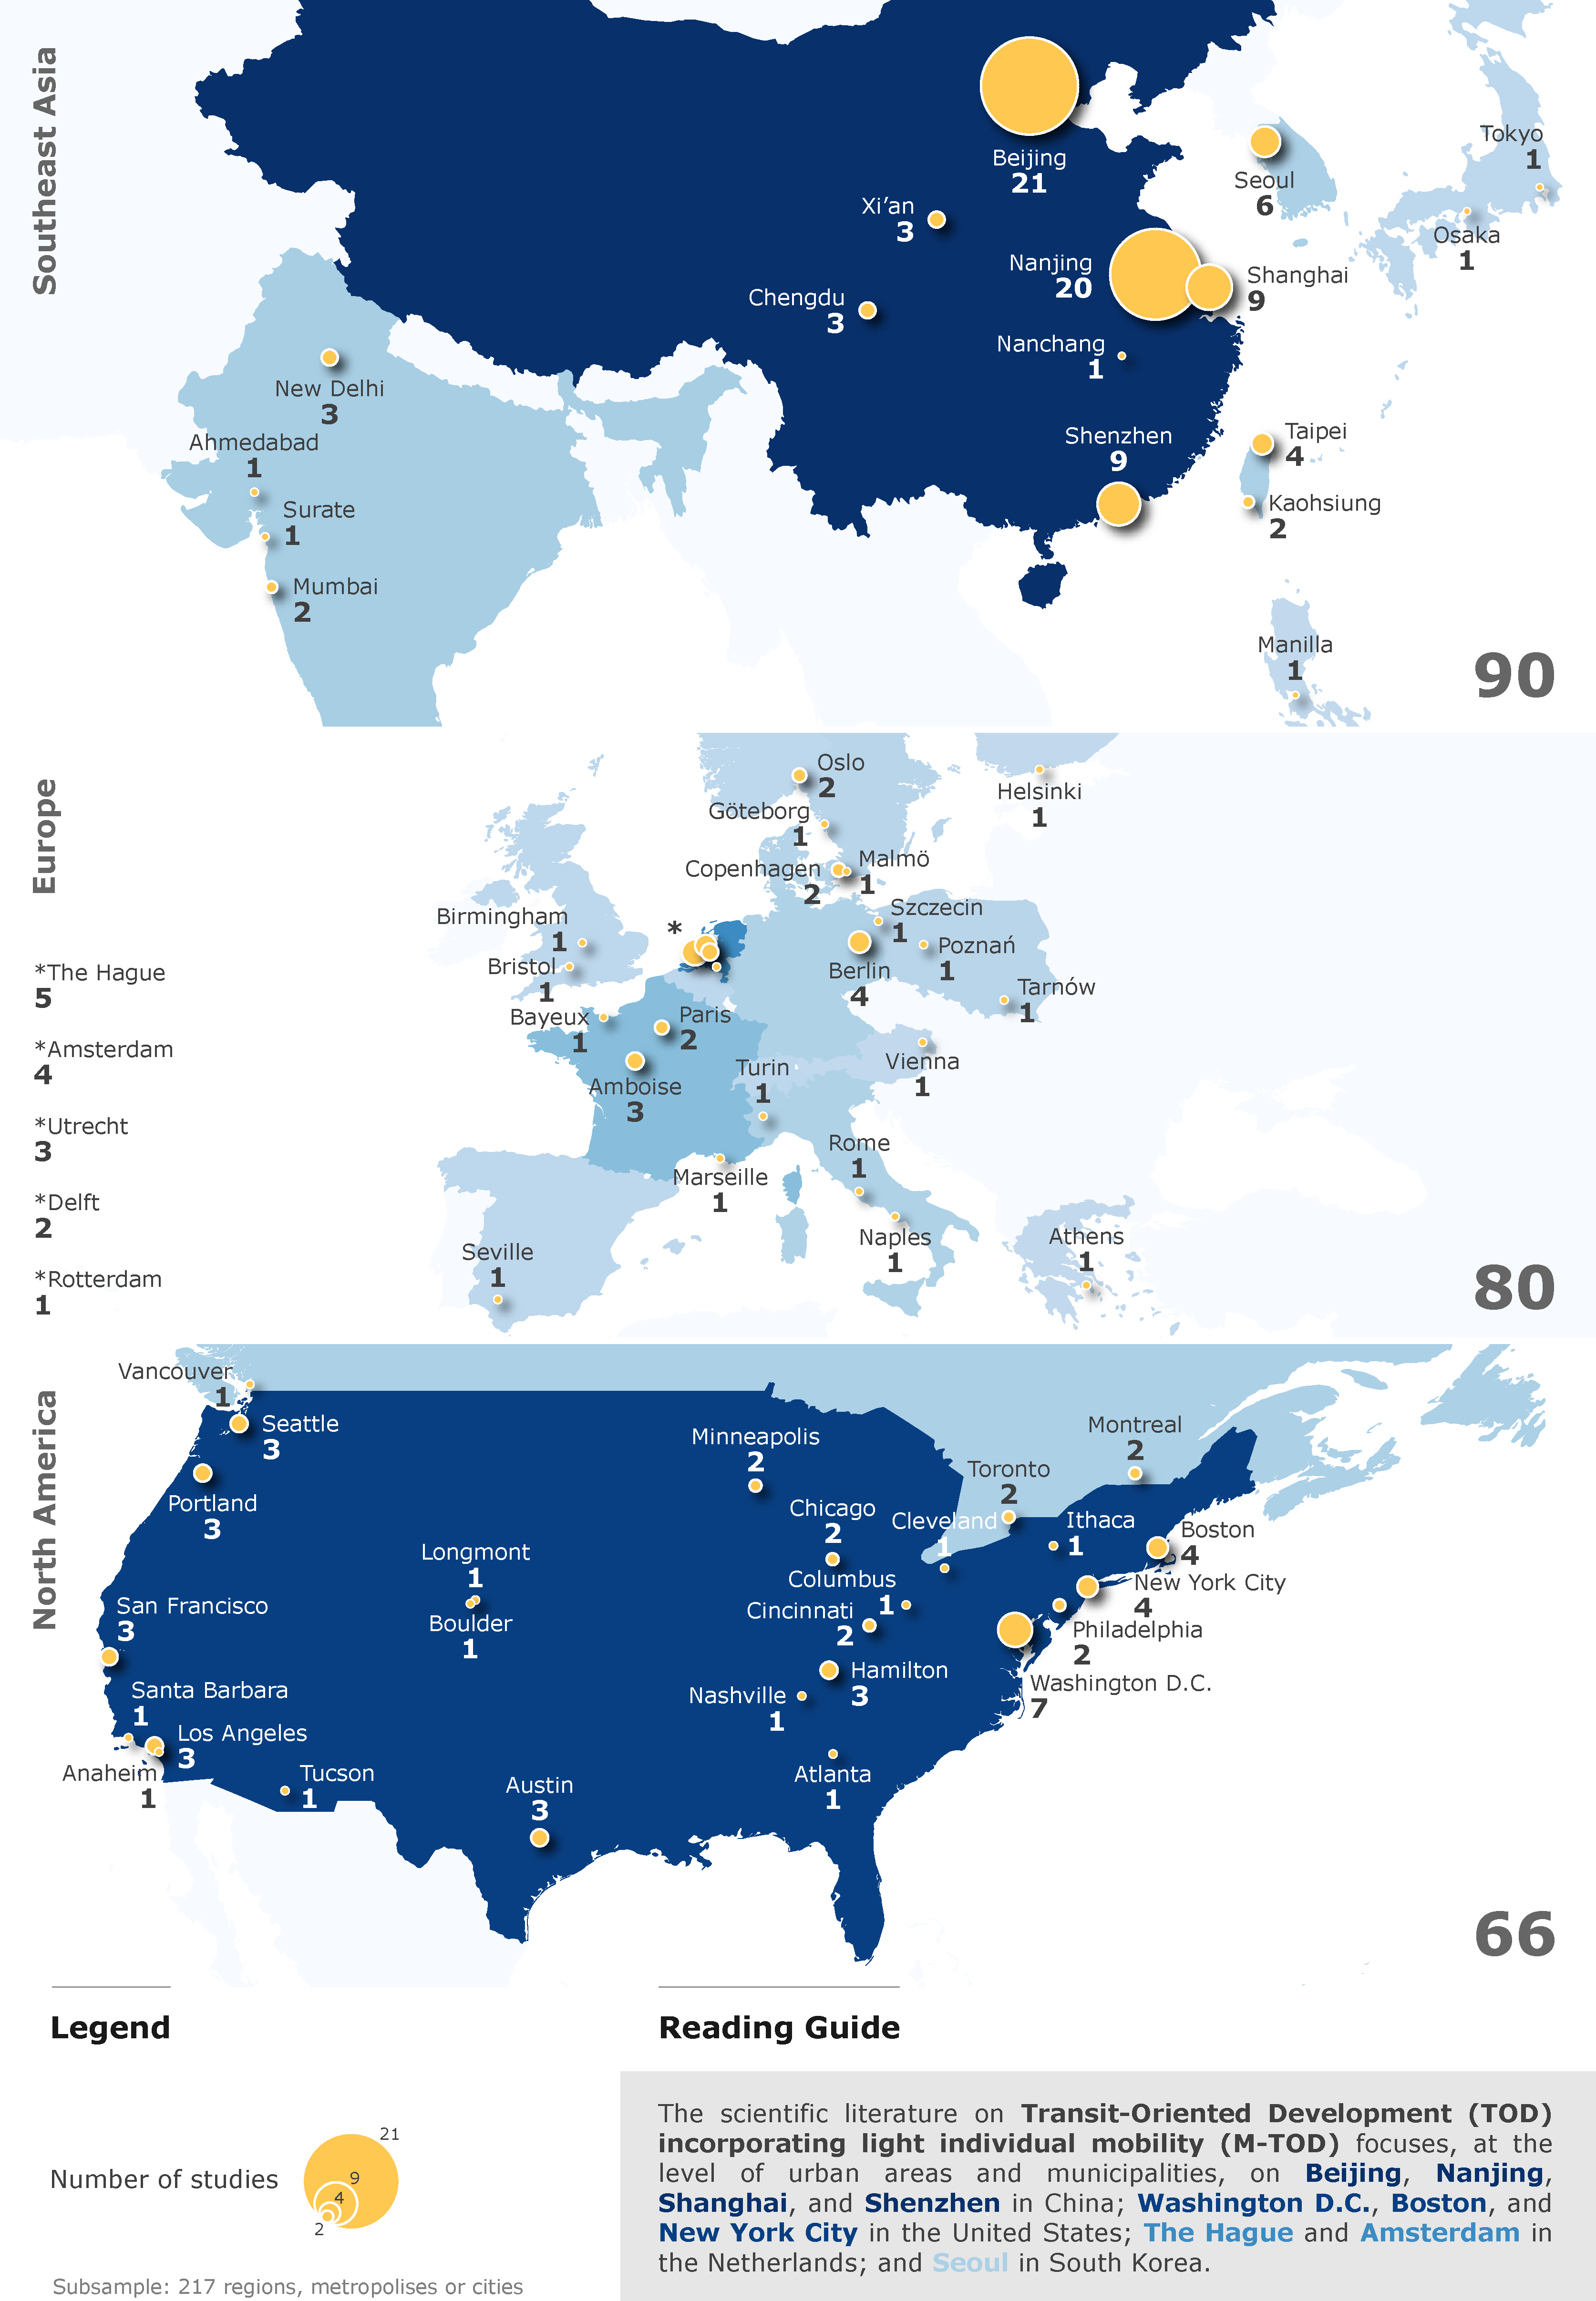
\includegraphics[width=1\columnwidth]{src/Figures/Chap-2/EN_RSL_Carte_Villes.pdf}}
        \vspace{5pt}
        \begin{flushleft}\scriptsize{
        \textcolor{blue}{Note:} The total number of contributions associated with each country and continent may exceed the values specific to each metropolitan area and city due to empirical works that have adopted a national scale.
        }\end{flushleft}
        \begin{flushright}\scriptsize{
        Author: \textcolor{blue}{Dylan Moinse (2023)}
        }\end{flushright}
    \end{carte}

    % micromobility and Public Transport by Continent
A second aspect addressed in this section focuses on the forms of intermodality studied in the analyzed documentation. As shown by the distributions displayed in \hyperref[fig-chap2:MIL-TC-continents]{Map~\ref{fig-chap2:MIL-TC-continents}} (page~\pageref{fig-chap2:MIL-TC-continents}), the various categories of light individual mobility and public transport are investigated unequally, depending on specific geographic areas. First, emerging light individual mobility is much more prominent in Asia, regarding bike-sharing, and in North America, for electric scooter services. Scientific publications selecting European settings primarily focus on conventional bicycles. Second, research on urban public transport systems is also concentrated in Asia, mainly with the metro, and in North America, with metro, tram, and bus systems. On a national scale, some countries specialize in specific forms of intermodality. Regarding bicycles and micromobility, we can particularly highlight the following list of countries:
\begin{customitemize}
    \item In the context of 126 survey sites on personal bicycles, 29 are in the United States, 28 in the Netherlands, 15 in China, 11 in France, 6 in India, and 4 in Canada. Additionally, 3 case studies each are found in South Africa, Germany, Australia, Brazil, Canada, Denmark, and Italy;
    \item Out of 60 locations addressing \acrshort{PBS}, 21 are in China, 17 in the United States, 5 in Taiwan, and 3 each in South Korea and the Netherlands;
    \item Regarding the list of 44 case studies on \acrshort{DBS}, only three countries are involved: 37 are located in China, 5 in the United States, and 2 in the Netherlands;
    \item Among the 20 empirical studies focused on the \acrshort{DESS} system, 13 are concentrated in the United States, and 2 in Germany.
\end{customitemize}
This statistical analysis can be compared with the \acrshort{SLR} conducted by \textcolor{blue}{\textcite[298]{zhang_built_2023}}\index{Zhang, Yushan|pagebf}\index{Kasraian, Dena|pagebf}\index{Wesemael, Pieter van|pagebf} on light individual mobility, which reports a higher proportion of studies on the \acrshort{DESS} system in Europe and on \acrshort{PBS} and \acrshort{DBS} in Asia, explained by the respectively developed markets.%%Translated%%

    % Figure MIL and TC by Continents
    \begin{figure}[h!]\vspace*{4pt}
        \caption{Forms of light individual mobility and public transport evaluated in the systematic literature review, by continent.}
        \label{fig-chap2:MIL-TC-continents}
        \centerline{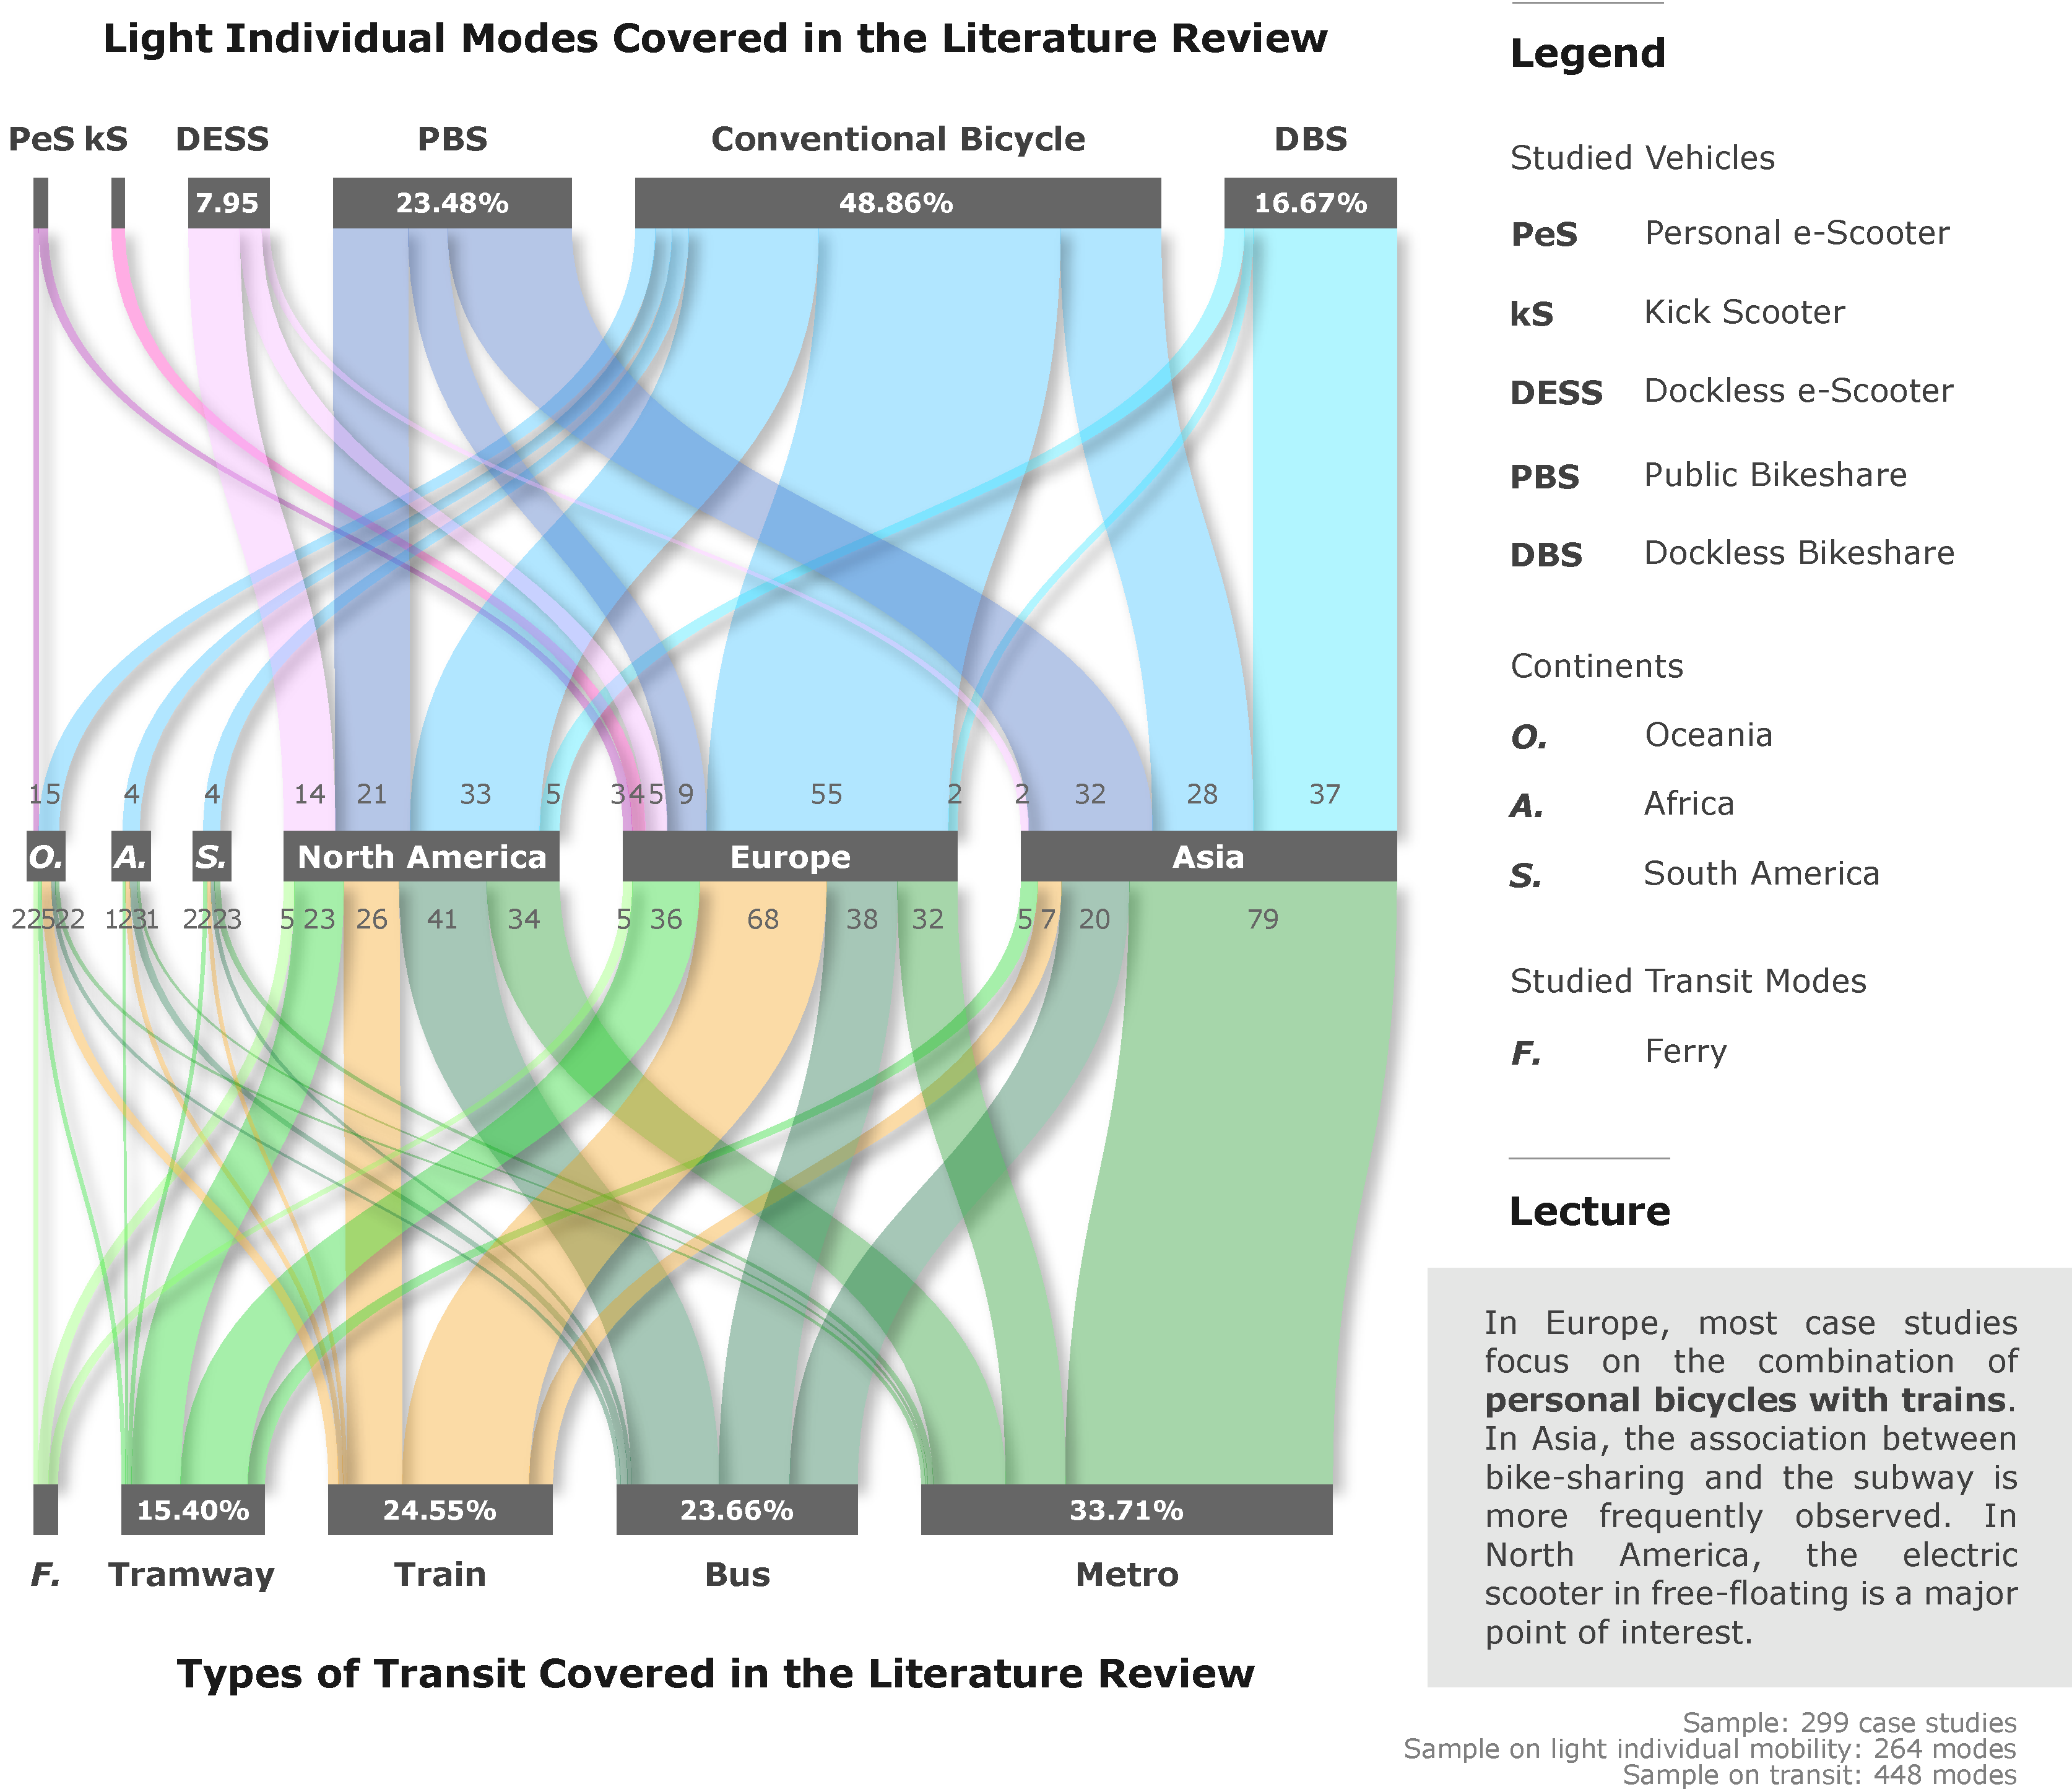
\includegraphics[width=1\columnwidth]{src/Figures/Chap-2/EN_RSL_MIL_TC_Continents.pdf}}
        \vspace{5pt}
        \begin{flushright}\scriptsize{
        Author: \textcolor{blue}{Dylan Moinse (2023)}
        %\\
        %Created with \Marque{Python}~and \Marque{Illustrator}
        }\end{flushright}
    \end{figure}

    % TC Multimodality
    Although the discernible distinction between different public transport systems is ambiguous when it comes to making international comparisons\footnote{~
    The ambiguity between metro and train in the context of international comparisons is inevitable due to geographical, cultural, and transport approach differences. Local trends and preferences, as well as technological and urban development, can blur the lines between metro and train, especially when comparing different regions.
}, a significant proportion of the academic contributions engage in simultaneous investigation of various modes of public transport. It is clear that, among the studies analyzed, the bus is examined in 66 scientific publications, similar to metro (55 occurrences), tram (53 occurrences), and train (51 occurrences), when considered alongside other modes of public transport. As for ferries, this maritime mode is consistently intertwined with other collective modes. Of the 72 documents addressing multiple collective modes simultaneously, 23 refer to the United States, 9 originate from China, and France and the Netherlands each contribute 6 studies.%%Translated%%

    % Minority Countries
As original contributions from regions that have been underexplored or omitted by the \acrshort{SLR}, we should mention the scientific works of \textcolor{blue}{\textcite[34]{bechstein_cycling_2010}}\index{Bechstein, Eva|pagebf}, \textcolor{blue}{\textcite[368]{cooke_relationship_2018}}\index{Cooke, Sean|pagebf}\index{Behrens, Roger|pagebf}\index{Zuidgeest, Mark|pagebf} and \textcolor{blue}{\textcite[2]{risimati_spatial_2021}}\index{Risimati, Brightnes|pagebf}\index{Gumbo, Trynos|pagebf}\index{Chakwizira, James|pagebf} in South Africa; \textcolor{blue}{\textcite[108]{quarshie_integrating_2007}}\index{Quarshie, Magnus|pagebf}\index{Morrison, Gregory~M.|pagebf}\index{Rauch, Sébastien|pagebf} in Ghana; \textcolor{blue}{\textcite[59]{souza_modelling_2017}}\index{Souza, Flavia de|pagebf}\index{La Paix Puello, Lissy|pagebf}\index{Brussel, Mark|pagebf}\index{Orrico, Romulo|pagebf}, \textcolor{blue}{\textcite[36]{arias_molinares_bike_2018}}\index{Arias Molinares, Daniela|pagebf}\index{Florez, Josefina|pagebf} and \textcolor{blue}{\textcite[40]{jansson_almeida_alternativas_2022}}\index{Jansson Almeida, Bárbara|pagebf} in Brazil; \textcolor{blue}{\textcite[206]{cervero_influences_2009}}\index{Cervero, Robert|pagebf}\index{Sarmiento, Olga~L.|pagebf}\index{Jacoby, Enrique|pagebf}\index{Gomez, Luis Fernando|pagebf}\index{Neiman, Andrea|pagebf} in Colombia; \textcolor{blue}{\textcite[6]{arbis_analysis_2016}}\index{Arbis, David|pagebf}\index{Hossein Rashidi, Taha|pagebf}\index{Dixit, Vinayak~V.|pagebf}\index{Vandebona, Upali|pagebf}, \textcolor{blue}{\textcite[2]{weliwitiya_factors_2017}}\index{Weliwitiya, Hesara|pagebf}\index{Rose, Geoff|pagebf}\index{Johnson, Marilyn|pagebf}, \textcolor{blue}{\textcite[396]{weliwitiya_bicycle_2019}}\index{Weliwitiya, Hesara|pagebf}\index{Rose, Geoff|pagebf}\index{Johnson, Marilyn|pagebf} and \textcolor{blue}{\textcite[5]{zhang_make_2023}}\index{Zhang, Mengyuan|pagebf}\index{Lee, Jinwoo Brian|pagebf} in Australia; or \textcolor{blue}{\textcite[17-22]{ensor_forecasting_2010}}\index{Ensor, Matt|pagebf}\index{Slason, Jonathan|pagebf}\index{Vallyon, Chris|pagebf} and \textcolor{blue}{\textcite[56-64]{ensor_mode_2021}}\index{Ensor, Matt|pagebf}\index{Maxwell,~O.|pagebf}\index{Bruce, Oliver|pagebf} in New Zealand.%%Translated%%

    % Chosen Scales/Perimeters (International/National/EPCI)
The focus on the geographical distribution of the study areas brings about an underlying reflection on the geographical scale preferred by empirical studies. Within the bibliographic corpus, comprising a total of 238 scientific works, four of them do not include case studies, instead adopting mathematical modeling approaches. Additionally, seven other studies only present a literature review, contrasting previous empirical research. Thus, 82\% of the research conducted on \acrshort{M-TOD} has chosen a geographical context based on an \acrfull{EPCI}, a municipality, or a local site. The remaining share is split between the national scale, at 11\%, and the regional scale, totaling 6\%\footnote{~
    It should be noted that this categorization only aims to provide a simplified framework for the various geographical scales, divided between national, regional, intercommunal, and municipal levels. However, this approach has limitations, as the delineation of geographical boundaries for a region or agglomeration varies depending on territorial contexts, leading to potential classification errors. For example, in 2019, the Île-de-France region spanned approximately 12,000 square kilometers and hosted 12 million inhabitants, whereas the Greater New York metropolitan area occupies 34,500 square kilometers with over 20 million inhabitants.
}. It is worth noting that the vast majority of state-of-the-art reviews adopt a national scale in order to compare different territories. Similarly, the \acrshort{SLR} by \textcolor{blue}{\textcite[298]{zhang_built_2023}}\index{Zhang, Yushan|pagebf}\index{Kasraian, Dena|pagebf}\index{Wesemael, Pieter van|pagebf} mentions a significant portion of studies on light individual mobility, where the geographical scope does not exceed municipal boundaries, and conversely, there is an almost complete absence of studies at the regional level.%%Translated%%

    % Types of Analyzed Territories 1 (Metropolises)
Further refining the geographical reference scale, it is interesting to note the plurality of agglomerations examined within the \acrshort{SLR}, in terms of their respective sizes. By focusing on the population of urban areas\footnote{~
    The comparative approach to populations is based on demographic data created by \textcolor{blue}{\textcite[]{schiavina_ghs-fua_2019}}\index{Schiavina, Marcello|pagebf}\index{Moreno-Monroy, Ana~I.|pagebf}\index{Maffenini, Luca|pagebf}\index{Veneri, Paolo|pagebf}. This data is grid-based population data that allows defining \acrfull{ZUF} globally \textcolor{blue}{\autocite[3]{moreno-monroy_metropolitan_2021}}\index{Moreno-Monroy, Ana~I.|pagebf}\index{Schiavina, Marcello|pagebf}\index{Veneri, Paolo|pagebf}.
}, we observe the three predominant continents in the study of \acrshort{M-TOD}. As shown in \hyperref[table-chap2:tailles-territoires-rsl]{Table~\ref{table-chap2:tailles-territoires-rsl}} (page~\pageref{table-chap2:tailles-territoires-rsl}), megacities\footnote{~
    \Commas{Megacities are urban agglomerations that, according to the United Nations' terminology, concentrate populations of 10 million inhabitants or more.} \textcolor{blue}{\autocite[]{geoconfluences_megapole_2023}}\index{Géoconfluences@\textsl{Géoconfluences}|pagebf}
} with populations over ten million people make up 43\% of the geographical areas present in the \acrshort{SLR}. This ranking is influenced by studies conducted in China (72\%) and, more generally, in East and Southeast Asia (88\%). Similarly, metropolises with international influence and populations exceeding three million inhabitants occupy a significant place in empirical research (27\%). These urban centers are mainly located in the United States (44\%) and specifically in North America (52\%). This phenomenon also echoes among metropolises of national or even international importance with populations over one million. These intermediate metropolises are notably found in Western Europe, making up 44\%, and are predominant when extending the scope to the entire European continent (62\%). Thus, the three types of urban areas mentioned encompass over 87\% of the investigations analyzed in the \acrshort{SLR}.%%Translated%%

    % Tableau types de territoires analysés RSL
% Table of analyzed territories RSL
%%Translated%%
        \begin{table}[h!]
    \centering
    \renewcommand{\arraystretch}{1.5}
    \resizebox{\columnwidth}{!}{
    \begin{tabular}{p{1\columnwidth}}
        %\hline
    \rule{0pt}{15pt} \small{\textbf{\textcolor{blue}{Agglomerations and Municipalities}}}\\
        \hline
    \small{\textbf{\textcolor{blue}{More than 10,000,000 inhabitants (88 references)}}}\\
\small{Beijing (21), Nanjing (19), Shenzhen (9), Shanghai (9), Seoul (6), New York City (4), Chengdu (3), Los Angeles (3), New Delhi (3), Xi'an (3), Chicago (2), Île-de-France (2), Mumbai (2), Bogotá (1), Johannesburg-Pretoria (1), Osaka (1), Manila (1), Rio de Janeiro (1)}\\
        \hdashline
    \small{\textbf{\textcolor{blue}{Between 3,000,000 and 10,000,000 inhabitants (53 references)}}}\\
\small{Washington D.C. (7), Berlin (4), Boston (4), Taipei (4), San Francisco (3), Seattle (3), Suzhou (3), Kaohsiung (2), Melbourne (2), Minneapolis (2), Montreal (2), Philadelphia (2), Toronto (2), Accra (1), Ahmedabad (1), Athens (1), Atlanta (1), Birmingham (1), Boulder (1), Cape Town (1), Nanchang (1), Porto Alegre (1), Rome (1), Surat (1), Sydney (1), Vienna (1)}\\
        \hdashline
    \small{\textbf{\textcolor{blue}{Between 1,000,000 and 3,000,000 inhabitants (33 references)}}}\\
\small{Rotterdam-The Hague (6), Amsterdam (4), Austin (3), Cincinnati (2), Cleveland (2), Copenhagen (2), Oslo (2), Auckland (1), Bristol (1), Columbus (1), Helsinki (1), Gutenberg (1), Aix-Marseille-Provence (1), Nashville (1), Orlando (1), Poznań (1), Seville (1), Tucson (1), Turin (1)}\\
        \hdashline
    \small{\textbf{\textcolor{blue}{Between 250,000 and 1,000,000 inhabitants (16 references)}}}\\
\small{Hamilton (3), Portland (3), Utrecht (3), Delft (2), Amstelland-Meerlanden (1), Eindhoven (1), Malmö (1), Mamelodi (1), Tarnow (1)}\\
        \hdashline
    \small{\textbf{\textcolor{blue}{Less than 250,000 inhabitants (8 references)}}}\\
\small{Amboise (3), Bayeux (1), El Monte (1), Ithaca (1), Longmont (1), Belgian municipalities between 30,000 and 200,000 inhabitants (1)}\\
        \hline
        \end{tabular}}
    \caption{Size of agglomerations and municipalities studied in the systematic literature review.}
    \label{table-chap2:tailles-territoires-rsl}
        \vspace{5pt}
        \begin{flushleft}\scriptsize{
        \textcolor{blue}{Reading:} Based on 198 studies including a geographical area, the systematic literature review primarily consists of agglomerations with more than 3,000,000 inhabitants.
        }\end{flushleft}
        \begin{flushright}\scriptsize
        Author: \textcolor{blue}{Dylan Moinse (2023)}
        \end{flushright}
        \end{table}%%Translated%%

% Types of territories analyzed 2 (regional metropolises)
For agglomerations with populations of less than one million inhabitants, the case studies in urban areas are primarily focused on Dutch intermunicipalities, specifically in the localities of Delft \textcolor{blue}{\autocites[113]{heinen_multimodal_2014}[5]{molin_bicycle_2015}}\index{Heinen, Eva|pagebf}\index{Bohte, Wendy|pagebf}\index{Molin, Eric|pagebf}\index{Maat, Kees|pagebf}, Amstelland-Meerlanden \textcolor{blue}{\autocite[46]{brand_assessing_2015}}\index{Brand, Judith Caroline|pagebf}, Eindhoven \textcolor{blue}{\autocite[724]{waerden_relation_2018}}\index{Waerden, Peter|pagebf}\index{Waerden, Jaap|pagebf}, and Utrecht \textcolor{blue}{\autocite[289]{kuijk_preferences_2022}}\index{Mil, Joeri~F.P. van|pagebf}\index{Leferink, Tessa~S.|pagebf}\index{Annema, Jan Anne|pagebf}\index{Oort, Niels van|pagebf}\index{Kuijk, Roy~J. van|pagebf}\index{Almeida Correia, Gonçalo Homem de|pagebf}\index{Oort, Niels van|pagebf}\index{Arem, Bart van|pagebf}. The United States also constitutes a relevant area for this research topic, with studies based in Portland \textcolor{blue}{\autocites[164]{krizek_assessing_2011}[400]{mcqueen_assessing_2022}[94]{singleton_exploring_2014}[265]{welch_long-term_2016}[83]{pucher_integrating_2009}}\index{Krizek, Kevin~J.|pagebf}\index{Stonebraker, Eric~W.|pagebf}\index{McQueen, Michael|pagebf}\index{Clifton, Kelly~J.|pagebf}\index{Singleton, Patrick~A.|pagebf}\index{Welch, Timothy~F.|pagebf}\index{Gehrke, Steven~R.|pagebf}\index{Wang, Fangru|pagebf}\index{Pucher, John|pagebf}\index{Buehler, Ralph|pagebf} and Anaheim, in the Greater Los Angeles Area \textcolor{blue}{\autocite[1579]{liu_simultaneous_2015}}\index{Liu, Yang|pagebf}\index{Zhu, Ning|pagebf}\index{Ma, Shou-feng|pagebf}. Similarly, Canadian territories contribute to this body of work, with scientific publications focused on the metropolitan area of Hamilton \textcolor{blue}{\autocites[2162]{chan_factors_2020}[375]{ravensbergen_biking_2018}}\index{Ravensbergen, Léa|pagebf}\index{Chan, Kevin|pagebf}\index{Farber, Steven|pagebf}\index{Buliung, Ron|pagebf}\index{Mendonca, Meaghan|pagebf}\index{Garg, Naren|pagebf}. As for rural and suburban territorial arrangements, French examples are numerous, marked by a series of studies conducted in the municipalities of Amboise \textcolor{blue}{\autocites[747]{midenet_modal_2018}[2729]{papon_evaluation_2017}[14-16]{papon_rapport_2015}}\index{Midenet, Sophie|pagebf}\index{Côme, Etienne|pagebf}\index{Papon, Francis|pagebf}\index{Beauvais, Jean-Marie|pagebf}\index{Midenet, Sophie|pagebf}\index{Côme, Etienne|pagebf}\index{Polombo, Nadine|pagebf}\index{Abours, Sylvie|pagebf}\index{Belton-Chevallier, Leslie|pagebf}\index{Soulas, Claude|pagebf} and Bayeux \textcolor{blue}{\autocite[2]{richer_service_2017}}\index{Richer, Cyprien|pagebf}, as well as in the former \acrfull{CC} of the Brie Boisée (now part of Île-de-France since 2017), in comparison with that of Carnelle Pays de France and Haute Vallée de Chevreuse \textcolor{blue}{\autocite[39]{stransky_periurbain_2019}}\index{Stransky, Vaclav|pagebf}.%%Translated%%

% International comparisons figure
\begin{figure}[h!]\vspace*{4pt}
    \caption{Comparisons between geographical areas in the bibliographic corpus of the systematic literature review.}
    \label{fig-chap2:comparaisons-internationales-rsl}
    \centerline{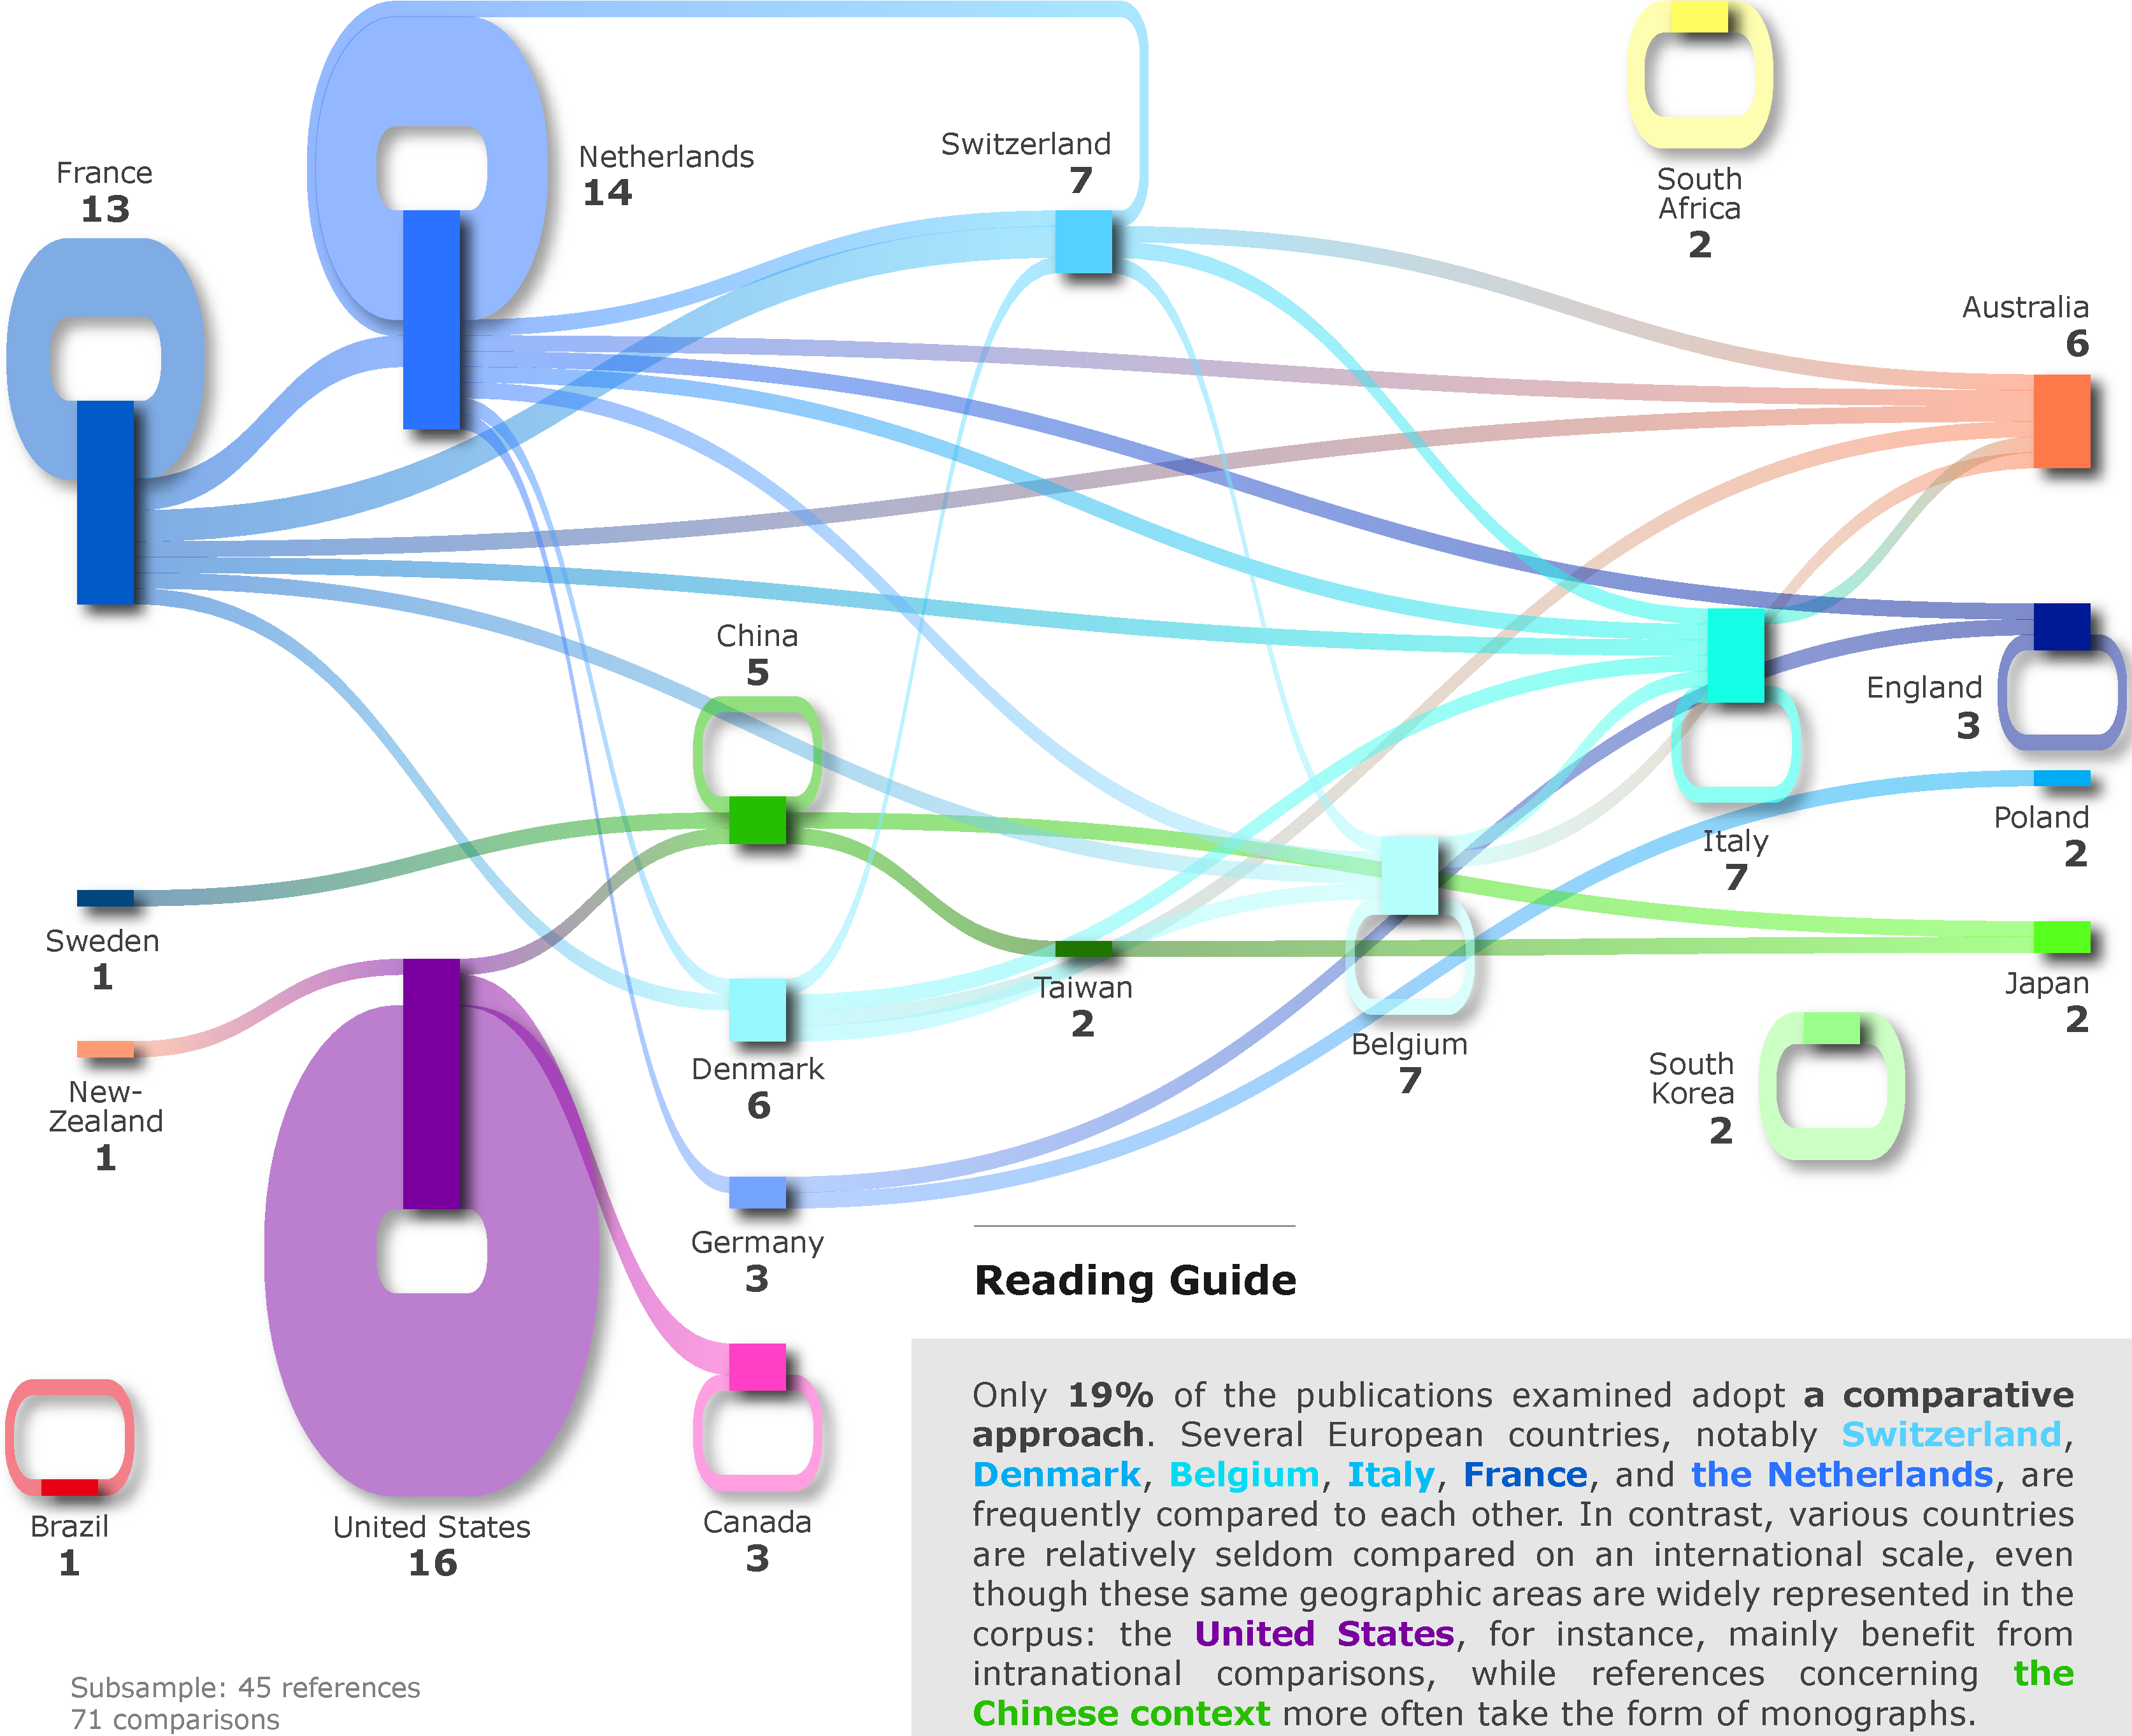
\includegraphics[width=1\columnwidth]{src/Figures/Chap-2/EN_RSL_Comparaisons_internationales.pdf}}
    \vspace{5pt}
    \begin{flushright}\scriptsize{
    %\\
    %Created with \Marque{Python}~and \Marque{Illustrator
    \textcolor{blue}{Note:} Only comparisons between different regions were considered in order to exclude urban areas with multiple local sites studied. The ring represents subnational comparisons, while the flows link the geographical areas in perspective.
    \\
    Author: \textcolor{blue}{Dylan Moinse (2023)}
    }\end{flushright}
\end{figure}

% International comparisons
While the literature on \acrshort{M-TOD} commonly adopts a comparative approach by selecting various study sites within a coherent political system, fewer studies make parallel comparisons between territories in different countries. In fact, it appears that 19\% of the publications reviewed focus on international or subnational comparisons. In the subset of 45 scientific papers dedicated to comparisons, 30 of them make comparisons between different \acrshort{EPCI}, while 11 others focus on the national level. As shown in \hyperref[fig-chap2:comparaisons-internationales-rsl]{Figure~\ref{fig-chap2:comparaisons-internationales-rsl}} (page~\pageref{fig-chap2:comparaisons-internationales-rsl}), certain countries are frequently compared, such as Switzerland, Denmark, Belgium, Italy, France, and the Netherlands \textcolor{blue}{\autocites[29-46]{abours_rapport_2015}[279-285]{sebban_complementarite_2003}[282-284]{martens_bicycle_2004}}\index{Abours, Sylvie|pagebf}\index{Midenet, Sophie|pagebf}\index{Soulas, Claude|pagebf}\index{Sebban, Annie-Claude|pagebf}\index{Martens, Karel|pagebf}, often with other European countries; or Japan, Taiwan, and China \textcolor{blue}{\autocite[212]{lin_built_2018}}\index{Lin, Jen-Jia|pagebf}\index{Zhao, Pengjun|pagebf}\index{Takada, Kazuyuki|pagebf}\index{Li, Shengxiao|pagebf}\index{Yai, Tetsuo|pagebf}\index{Chen, Chi-Hao|pagebf}. It is worth noting that there are also two intercontinental comparisons, conducted by \textcolor{blue}{\textcite[4]{hamidi_shaping_2020}}\index{Hamidi, Zahra|pagebf}\index{Zhao, Chunli|pagebf} who studied the urban areas of Beijing, Göteborg, and Malmö in China and Sweden; and by \textcolor{blue}{\textcite[13]{hua_transfer_2022}}\index{Hua, Mingzhuang|pagebf}\index{Pereira, Francisco Camara|pagebf}\index{Jiang, Yu|pagebf}\index{Chen, Xuewu|pagebf} who examined the Chinese and U.S. cities of Nanjing and Chicago.%%Translated%%

% Subnational comparisons
In contrast, some countries are rarely put into perspective, even though they are occasionally compared in small proportions (see \hyperref[fig-chap2:comparaisons-internationales-rsl]{Figure~\ref{fig-chap2:comparaisons-internationales-rsl}}, page~\pageref{fig-chap2:comparaisons-internationales-rsl}). For instance, the United States, except for some comparisons with Canada \textcolor{blue}{\autocites[11-16]{ensor_forecasting_2010}[7]{schneider_integration_2005}[83]{pucher_integrating_2009}}\index{Ensor, Matt|pagebf}\index{Slason, Jonathan|pagebf}\index{Vallyon, Chris|pagebf}\index{Schneider, Robert|pagebf}\index{Pucher, John|pagebf}\index{Buehler, Ralph|pagebf}, mainly benefit from subnational comparisons. Some countries have only been involved in internal comparisons between different regions within the same geographical entity. In South Africa, \textcolor{blue}{Eva} \textcolor{blue}{\textcite[34]{bechstein_cycling_2010}}\index{Bechstein, Eva|pagebf} conducts a comparative study between the \Commas{\textsl{townships}}\footnote{~
    \Commas{In South Africa, since the \textsl{apartheid} regime, the term \textsl{township} refers to areas inhabited by people of color (black and \textsl{coloured}). [\dots] Over time, the term has come to describe poor, degraded, and unsanitary housing areas, approaching the definition of a slum.} \textcolor{blue}{\autocite{geoconfluences_township_2023}}\index{Géoconfluences@\textsl{Géoconfluences}|pagebf}.
} of Mamelodi and Nellmapius (Tshwane), similarly to \textcolor{blue}{\textcite[368]{cooke_relationship_2018}}\index{Cooke, Sean|pagebf}\index{Behrens, Roger|pagebf}\index{Zuidgeest, Mark|pagebf} who compare the metropolitan municipalities of Johannesburg, Cape Town, Tshwane, Nelson Mandela Bay, and eThekwini. In South Korea, research by \textcolor{blue}{\textcite[43, 980]{lee_strategies_2010, lee_bicycle-based_2016}}\index{Lee, Jaeyeong|pagebf}\index{Shin, Hee-Cheol|pagebf}\index{Lee, Jaeyeong|pagebf}\index{Choi, Keechoo|pagebf}\index{Leem, Yountaik|pagebf} focuses on a comparative analysis between the metropolitan regions of Seoul and Daejeon.%%Translated

% Few comparisons
In contrast, \hyperref[fig-chap2:comparaisons-internationales-rsl]{Figure~\ref{fig-chap2:comparaisons-internationales-rsl}} (page~\pageref{fig-chap2:comparaisons-internationales-rsl}) reveals the underrepresentation, or even absence, of certain countries that are well-studied in the \acrshort{SLR}. The most striking case is that of China, where the vast majority of research uses a monographic approach, focusing solely on a single agglomeration. However, it should be noted that these studies are not necessarily non-comparative \textcolor{blue}{\autocite[30-31]{gueranger_monographie_2012}}\index{Guéranger, David|pagebf}. For example, the study conducted by \textcolor{blue}{\textcite[77]{liu_solving_2012}}\index{Liu, Zhili|pagebf}\index{Jia, Xudong|pagebf}\index{Cheng, Wen|pagebf} carries out two case studies in the districts of Dongcheng and Haidian, in Beijing, after conducting an exhaustive analysis of the \acrshort{PBS} system around subway and bus stops in the capital. By excluding comparisons within the same urban area due to methodological constraints related to the normalization of geographical areas, this chart masks the analogical reasoning present at the submunicipal level.%%Translated%%

% Conclusion
In summary, this section dedicated to the state of international scientific literature on \acrshort{M-TOD} has examined both the analysis of the metadata of the collected scientific publications, the lexical patterns used to describe the research topic, as well as the chronological trends and the geographical distribution of the investigations conducted. After analyzing the documentation from the metadata perspective, the following section will address the conceptual and methodological frameworks of the scientific literature on \acrshort{M-TOD}, focusing on the theoretical foundations, the evaluation of approaches, and the types of analysis employed in the investigations.%%Translated%%

% 2.2.2. Concepts, methods, types of analysis
\needspace{1\baselineskip} % Reserve space
\subsection{Conceptual and Methodological Frameworks of the Corpus
    \label{chap2:cadres-conceptuels-methodologiques}
    }

% Introduction
This section is dedicated to presenting and comparing the various theoretical foundations and approaches used in the scientific literature. The following questions have been considered in this analysis:
    \begin{customitemize}
        \item What are the main theoretical frameworks employed in the selected documentation? How have these theoretical choices been applied to the research questions?
        \item Can we identify any evolution of the theoretical frameworks adopted over time? Do these trends reflect certain disciplinary directions or advancements? What criticisms have the authors raised regarding the theoretical frameworks used?
        \item What data collection methods have been used? What data analysis techniques have been applied?
        \item How have the authors addressed the constraints and limitations of the data collection and analysis methods used?
    \end{customitemize}%%Translated%%

% Plan announcement
This subsection aims to introduce the theoretical frameworks found in the scientific literature (\hyperref[chap2:fondements-theoriques]{Subsection~2.2.1}, page~\pageref{chap2:fondements-theoriques}), prior to evaluating the data collection processes (\hyperref[chap2:methodes-collecte-donnees]{Subsection~2.2.2}, page~\pageref{chap2:methodes-collecte-donnees}) and the data analysis methods (\hyperref[chap2:demarches-types-analyses]{Subsection~2.2.3}, page~\pageref{chap2:demarches-types-analyses}) employed to study \acrshort{M-TOD}.%%Translated%%

% 2.2.2.1. Mobilized Concepts, TOD
\needspace{1\baselineskip} % Reserve space
\subsubsection*{Theoretical Foundations
    \label{chap2:fondements-theoriques}
    }

% Theoretical frameworks description
In the 102 scientific articles analyzed in the context of the \acrshort{SLR}, the concept of \acrshort{TOD} is predominant, being cited in 55 studies. Among these, 53 articles explicitly discuss \acrshort{TOD}, with nine of them specifically relying on the principles of the \Commas{Ds} to structure their analysis. Four studies are based on an analytical approach of the \Commas{5Ds}, three on the \Commas{3Ds}, one on the \Commas{4Ds}, and another on the \Commas{6Ds}\footnote{~
    In the commonly accepted order in the scientific literature on \acrshort{TOD}, and as presented in the \hyperref[chap1:tod-presentation-generale-definition]{section on the definition of \textsl{Transit-Oriented Development}} (page~\pageref{chap1:tod-presentation-generale-definition}) of \hyperref[chap1:titre]{Chapter~1} (page~\pageref{chap1:titre}), the \Commas{\acrshort{7Ds}} are composed as follows: Density (\(D1\)), Diversity (\(D2\)), Design (\(D3\)), Destination Accessibility (\(D4\)), Distance to Transit (\(D5\)), Demand Management (\(D6\)), and Demographics (\(D7\)).
}. Four articles integrate a revised version of \acrshort{TOD} that closely reflects this chapter, focusing on \acrshort{M-TOD}. The significant place of \acrshort{TOD} in the literature is, however, influenced by its inclusion in our research formula during the database collection. In addition to \acrshort{TOD}, two other concepts frequently emerge: the \Commas{first and last miles,} mentioned 24 times, and \Commas{multimodal accessibility,} discussed in 20 articles. Other concepts are also present, such as \Commas{car dependency} (four mentions), \acrfull{MaaS} (four mentions), \Commas{social inclusivity} (four mentions), and \Commas{planned behavior theory} (two mentions).%%Translated%%

% Focus on M-TOD
In fact, a significant number of publications address the concept of \acrshort{TOD} without explicitly mentioning it. Similarly, although rarely cited, the concept of \acrshort{M-TOD} is intrinsically linked to the academic corpus that examines the integration of light individual mobility with public transport networks, while articulating issues related to mobility and urban development. First, it is worth mentioning the study by \textcolor{blue}{\textcite{lee_bicycle-based_2016}}\index{Lee, Jaeyeong|pagebf}\index{Choi, Keechoo|pagebf}\index{Leem, Yountaik|pagebf} that led to the conceptualization of \acrshort{B-TOD}, based on an investigation exploring the relationship between bicycles and the subway in Seoul and Daejeon. Additionally, three studies using \acrshort{B-TOD} focus on different objects and geographical contexts: one in Nanjing examining bicycles, \acrshort{PBS}, and the subway \textcolor{blue}{\autocite{ji_public_2017}}\index{Ji, Yanjie|pagebf}\index{Fan, Yingling|pagebf}\index{Ermagun, Alizera|pagebf}\index{Cao, Xuening|pagebf}\index{Wang, Wei|pagebf}\index{Das, Kirti|pagebf}; another in Kaohsiung between \acrshort{PBS} and the subway \textcolor{blue}{\autocite{cheng_expanding_2018}}\index{Cheng, Yung-Hsiang|pagebf}\index{Li, Yi-Chun|pagebf}; and the last studying the link between bicycles and buses in the cities of Cape Town, Tshwane, Joburg, Nelson Mandela Bay, and eThekwini \textcolor{blue}{\autocite{cooke_relationship_2018}}\index{Cooke, Sean|pagebf}\index{Behrens, Roger|pagebf}\index{Zuidgeest, Mark|pagebf}. The diversity of theoretical approaches adopted reflects the methodological plurality aimed at exploring the interactions between bicycles, micromobility, and public transport.%%Translated%%

% 2.2.2.2. Methods, data sources, and sample
\needspace{1\baselineskip} % Reserve space
\subsubsection*{Evaluation of Data Collection Methods
    \label{chap2:methodes-collecte-donnees}
    }

% Detailed data sources: big data
The analysis of the data sources used in the documentation led to the identification of 17 types of data collection methods, classified into five independent categories. The majority of the scientific productions rely on the use of open data (29.15\%) and usage data (23.87\%), which can be grouped under the technical concept of \textsl{Big Data}\footnote{~
    In the context of mobility, \textsl{Big Data} refers to the collection and processing of a public or private database generated by a transport system, vehicle, users themselves, or other available sources. This technique for collecting real-time quantitative data is made possible by the emergence of technologies such as sensors embedded in vehicles, counters, smartphones, or the deployment of digital tools.
}, followed by surveys (24.62\%) and secondary data analysis from databases (16.58\%). The mobility flows available online thus represent 53.02\% of the data sources used and primarily correspond to \textsl{Open Data}\footnote{~
    \textsl{Open Data} refers, in the case of this \acrshort{SLR}, to the public data-sharing policy related to urban planning and mobility. These open data, provided by local authorities and public agencies, include various information related to urban planning, land use, infrastructure, demographics, and other aspects of territorial management.
} (22.54\%), \acrfull{API}\footnote{~
    An \acrshort{API} is a computer interface that connects applications and services with mobility systems in a standardized manner. \acrshort{API}\textcolor{blue}{s} facilitate the exchange of data between mobility service providers and third-party applications, such as vehicle location, status, and availability in real-time, unlocking vehicles, and the billing process for a trip made. All the data generated and exchanged allow companies to access aggregated data on vehicle usage and integrate it.
} (11.72\%), and mobility flows related to \acrshort{PBS} systems, called \acrfull{GBFS}\footnote{~
    \acrshort{GBFS} defines a standardized data format specifically designed for \acrshort{PBS} systems, aimed at providing real-time information about the mobility service and promoting interoperability and transparency.
} (9.02\%) and public transport, \acrfull{GTFS}\footnote{~
    \acrshort{GTFS} is a standardized file format, initially called the \Commas{\textsl{Google Transit Feed Specification}}, used to describe public transport networks. This includes routes, stop points, time schedules, and ridership data. This standardization aims to facilitate the integration of these open data into mapping and route planning tools. For this purpose, public transport agencies provide these standardized formats, targeting both third-party application developers and users.
} (6.85\%). We also find some data collection techniques classified under open and usage data, such as extracting mobility data from multimodal maps, around 2.16\%, or \acrshort{GPS} data (\textsl{Global Positioning System}), at 1.89\%.%%Translated%%

% Detailed data sources: qualitative methods
Beyond this data collection method related to \textsl{Smart Data}, a second range emerges associated with field surveys, through questionnaires (20.47\%), interviews (2.80\%), and observations (1.98\%). These techniques, rooted in the research practices of geography and sociology, are driven by the implementation of online questionnaires (11.45\%), face-to-face (7.66\%), and postal (1.35\%) surveys, as well as individually (1.71\%) or collectively (1.08\%) conducted interviews and direct observation sessions (1.98\%). The plurality of data collection methods is lastly reflected in the exploitation and reinterpretation of pre-existing public surveys (14.52\%) and the synthesis of previous materials (0.81\%).%%Translated%%

% Data sources by continent
By intertwining the data collection and processing methods used in scientific productions with the geographical context of the areas examined, differences in the use of data sources emerge (see \hyperref[fig-chap2:sources-donnees-rsl]{Figure~\ref{fig-chap2:sources-donnees-rsl}}, page~\pageref{fig-chap2:sources-donnees-rsl}). In this regard, we observe that Asian territories show a marked propensity for exploiting open data and usage data. This trend is more specifically manifested through the use of digital data from geographical sources, such as \textsl{Open Data}, \acrshort{API}, \acrshort{GBFS}, and multimodal maps\footnote{~
    A multimodal card, or \textsl{Smart Card}, refers to a card that integrates and displays information about several different transport modes within a single interface. By combining this information into one card, it can automatically collect anonymous data on user movements across a transport network, generally integrating train systems, urban public transport, and \acrshort{PBS}.
}. Similarly, online questionnaire surveys stand out for their prevalence across the three considered continents, whereas face-to-face questionnaires are more commonly used in Asian contexts. In parallel, interviews and observations, as well as secondary analysis of public surveys and literature reviews, are approaches more pronounced in North America and Europe.%%Translated%%

% Figure data sources RSL
\begin{figure}[h!]\vspace*{4pt}
    \caption{An imbalanced use of data collection methods according to geographical contexts, urban size, and the type of light individual mobility studied in the systematic literature review.}
    \label{fig-chap2:sources-donnees-rsl}
    \centerline{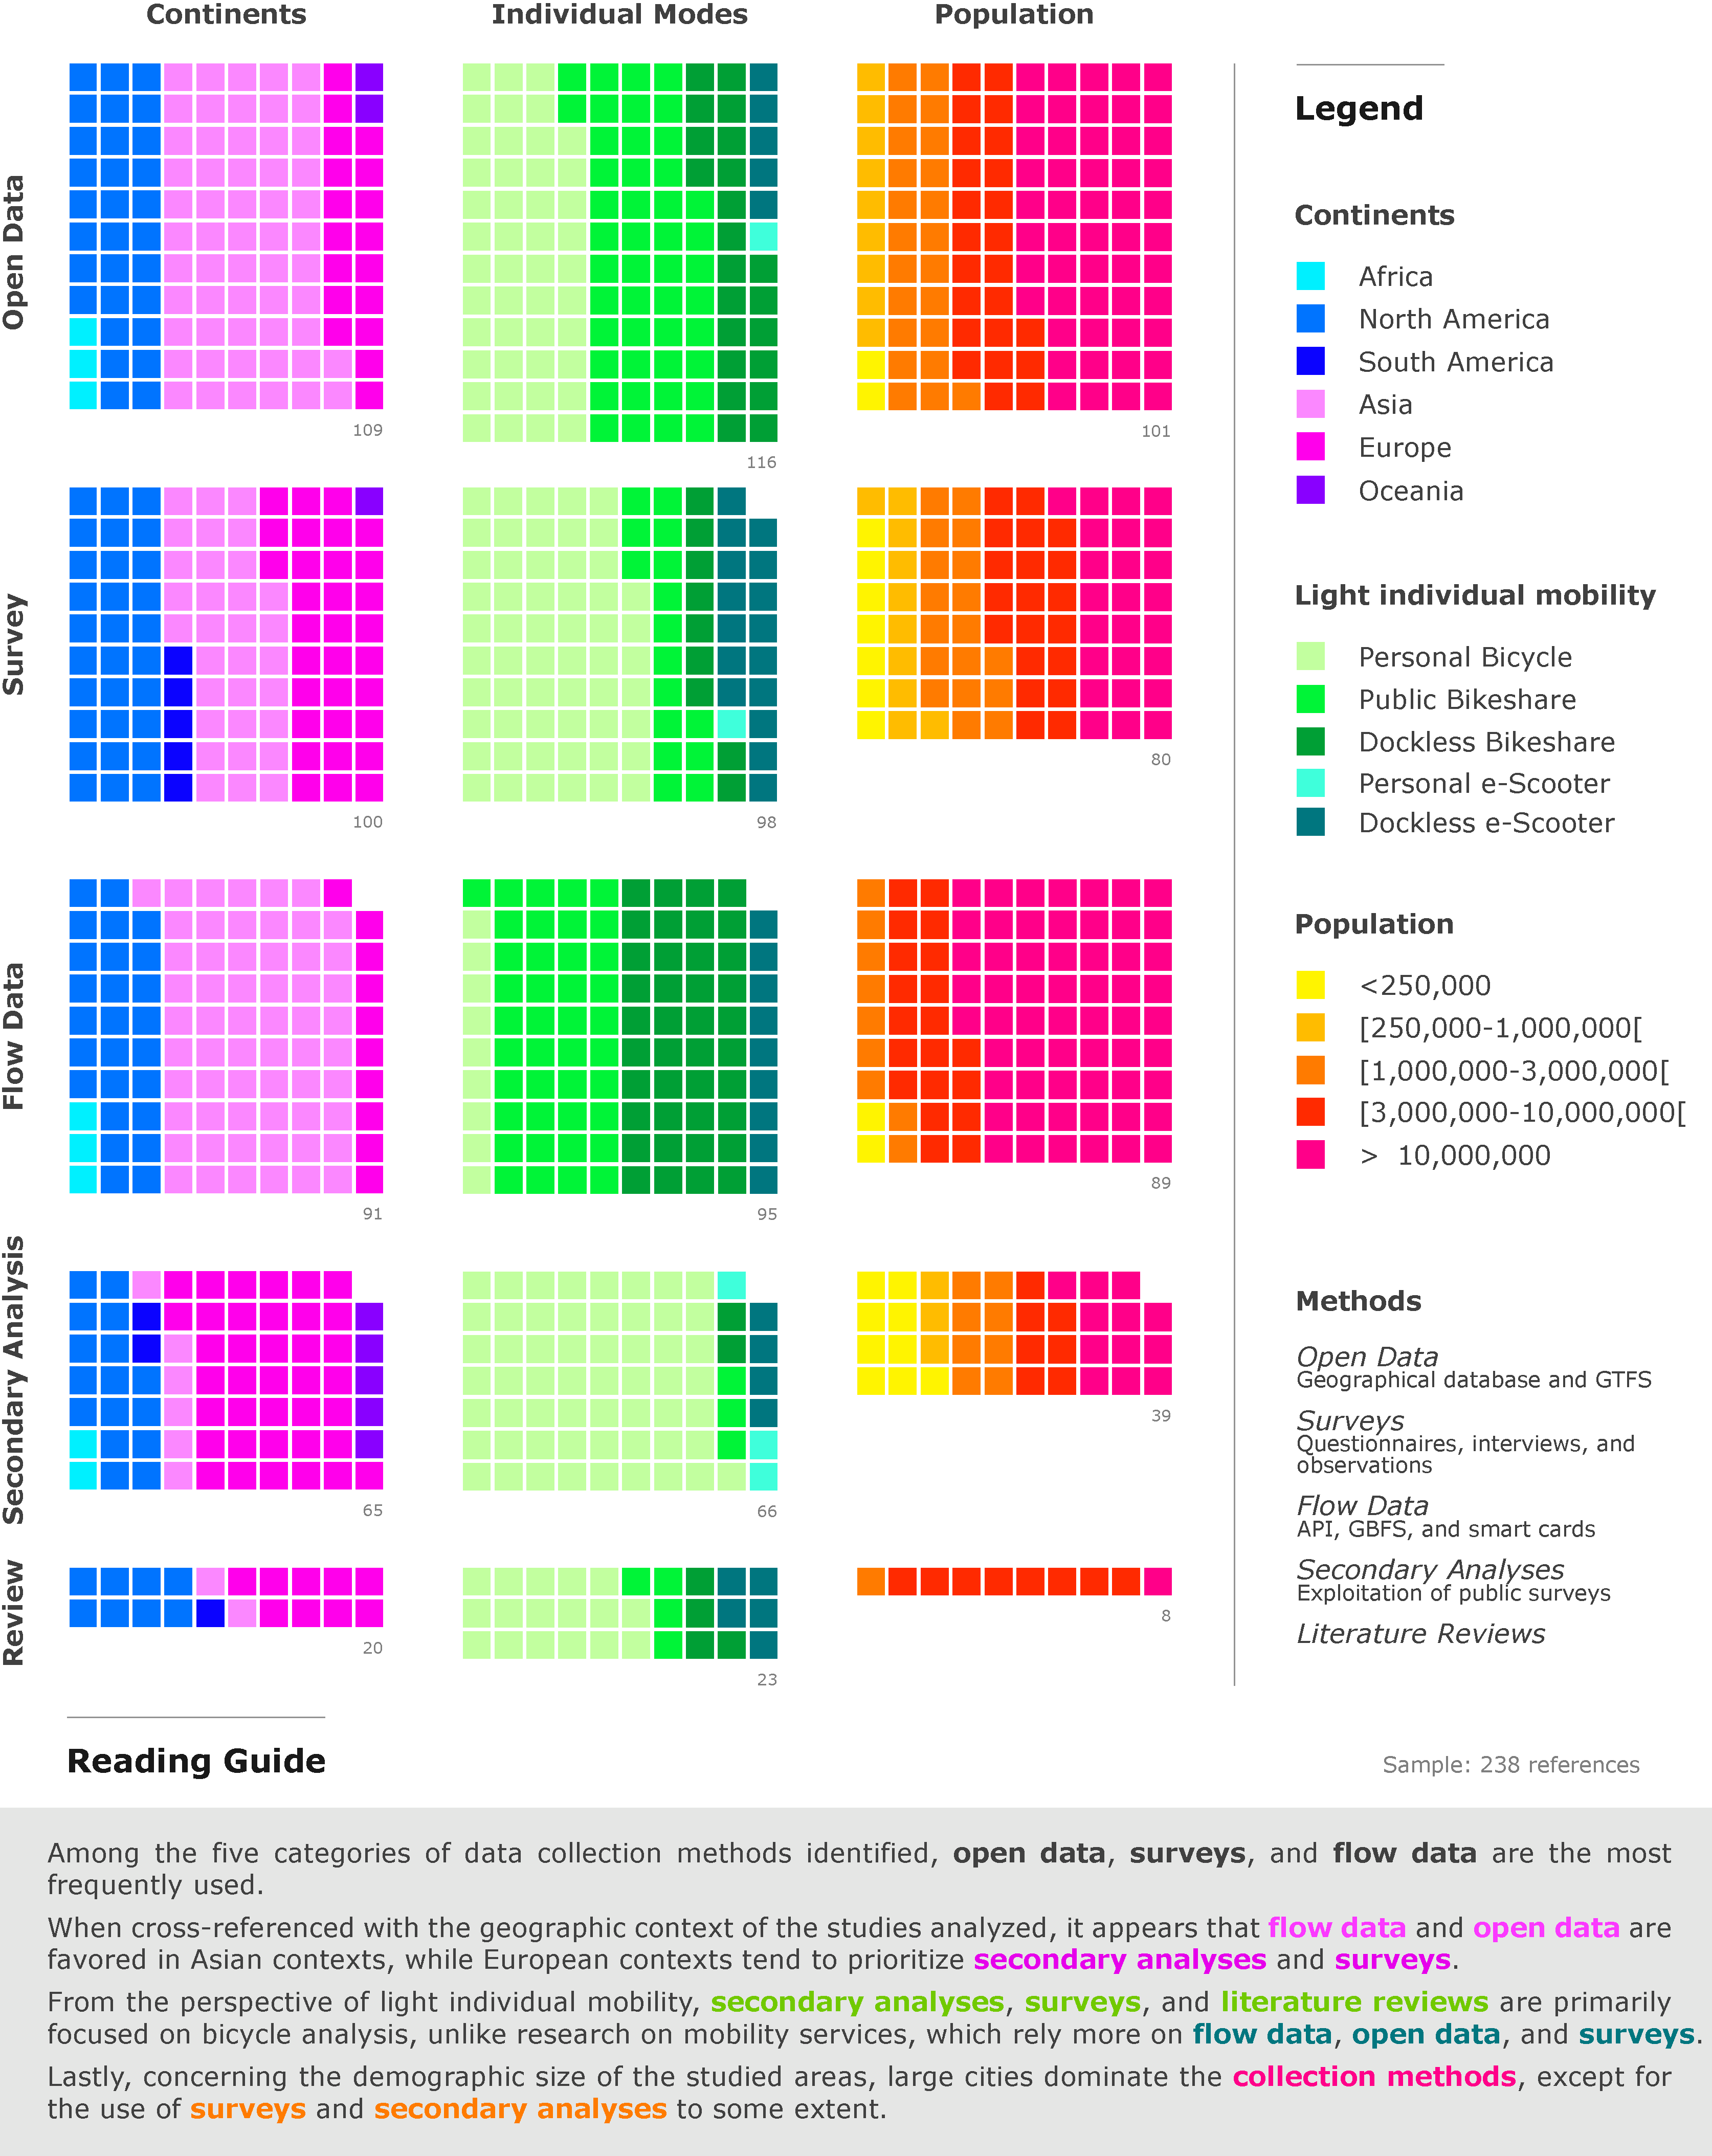
\includegraphics[width=1\columnwidth]{src/Figures/Chap-2/EN_RSL_Sources_donnees.pdf}}
    \vspace{5pt}
    \begin{flushright}\scriptsize{
    Author: \textcolor{blue}{Dylan Moinse (2023)}
    %\\
    %Created with \Marque{Excel}~and \Marque{Illustrator}
    }\end{flushright}
\end{figure}

% Data sources by urban agglomeration size
In a broader perspective, this methodological exploration reveals how urban size can influence distinct modes of investigation regarding empirical access to the field and information. By examining the typology of intermunicipalities, it becomes possible to identify patterns that suggest certain strategies for exploiting available data on the study areas. Thus, \hyperref[fig-chap2:sources-donnees-rsl]{Figure~\ref{fig-chap2:sources-donnees-rsl}} (page~\pageref{fig-chap2:sources-donnees-rsl}) highlights an overrepresentation of megacities within \textsl{Big Data}, with particular emphasis on \acrshort{API} and \acrshort{GBFS}. This predominance results from the concentration of bicycle and shared micromobility services, whether equipped with parking infrastructures or operating without them. In contrast, the data available regarding land use and public transport networks are more evenly distributed. Regarding the implementation of surveys through questionnaires, it is noteworthy that cities with fewer than three million inhabitants make greater use of online questionnaires. Agglomerations of at least 250,000 inhabitants tend to favor face-to-face questionnaires. Furthermore, secondary analysis of public surveys proves to be a preferred option in a significant proportion of smaller demographic agglomerations. This statistical interpretation can be explained by the differences in resource availability according to the specificities of the geographical areas. Indeed, massive data on a given territory are more rarely compiled in sparsely populated areas, and surveys help address this situation while being more accessible and less time-consuming.%%Translated%%

% Data sources by micromobility
The analysis of data collection methods has been cross-referenced with the forms of light individual mobility as they are addressed in the scientific corpus. While personal and intermodal bicycle use is primarily studied through face-to-face questionnaires or secondary analysis, the study of shared bicycles and micromobility relies heavily on the use of \textsl{Big Data}. On one hand, the examination of the \acrshort{PBS} system largely revolves around data generated by \acrshort{GBFS}. On the other hand, the investigation of \acrshort{DBS} and \acrshort{DESS} services is primarily based on the exploitation of \acrshort{API} (see \hyperref[fig-chap2:sources-donnees-rsl]{Figure~\ref{fig-chap2:sources-donnees-rsl}}, page~\pageref{fig-chap2:sources-donnees-rsl}). Unlike light shared mobility, which generates a large amount of real-time data, data on personal bicycles is more difficult to access in the form of massive data. Research on this mode of individual transport seems to focus on pre-existing surveys or field surveys in direct interaction with users.%%Translated%%

% Data sources examples face-to-face questionnaire
As an example, we can cite research on personal bicycle use and the use of face-to-face questionnaires by \textcolor{blue}{\textcite[1696]{cheng_evaluating_2012}}\index{Cheng, Yung-Hsiang|pagebf}\index{Liu, Kuo-Chu|pagebf} in association with the subway in Kaohsiung (386 responses), by \textcolor{blue}{\textcite[41]{jansson_almeida_alternativas_2022}}\index{Jansson Almeida, Bárbara|pagebf} with the subway in Porto Alegre (212 responses), by \textcolor{blue}{\textcite[183]{pan_intermodal_2010}}\index{Pan, Haixiao|pagebf}\index{Shen, Qing|pagebf}\index{Xue, Song|pagebf} on bicycles and \acrfull{e-Bike} with the subway in Shanghai (600 responses), by \textcolor{blue}{\textcite[7]{bauer_influence_2021}}\index{Bauer, Marek|pagebf}\index{Kisielewski, Piotr|pagebf} with the train and bus in Tarnow (501 responses), by \textcolor{blue}{\textcite[685, 4]{rastogi_travel_2003, rastogi_willingness_2010}}\index{Rastogi, Rajat|pagebf}\index{Krishna Rao,~K.~V.|pagebf} on walking and cycling with the train in Mumbai (1,449 responses), by \textcolor{blue}{\textcite[2]{rijsman_walking_2019}}\index{Rijsman, Lotte|pagebf}\index{Oort, Niels van|pagebf}\index{Ton, Danique|pagebf}\index{Hoogendoorn, Serge|pagebf}\index{Molin, Eric|pagebf}\index{Teijl, Thomas|pagebf} on walking and cycling with the tram in The Hague (629 responses), or by \textcolor{blue}{\textcite[192]{sherwin_practices_2011}}\index{Sherwin, Henrietta|pagebf}\index{Parkhurst, Graham|pagebf}\index{Robbins, Derek|pagebf}\index{Walker, Ian|pagebf} who combine the questionnaire and direct observation on bicycles with the train in Bristol (135 responses).%%Translated%%

% Data sources examples online questionnaire
Studies conducted using online questionnaires also show an imbalanced distribution in favor of personal bicycle use, as seen in the publications of \textcolor{blue}{\textcite[724]{waerden_relation_2018}}\index{Waerden, Peter|pagebf}\index{Waerden, Jaap|pagebf} on the combination of bicycles with trains in Eindhoven (415 responses), \textcolor{blue}{\textcite[5, 488]{la_paix_puello_train_2016, la_paix_puello_role_2021}}\index{La Paix Puello, Lissy|pagebf}\index{Geurs, Karst~T.|pagebf} with trains in the Rotterdam-The Hague metropolitan area and Randstad South (1,524 responses), \textcolor{blue}{\textcite[267]{krygsman_multimodal_2004}}\index{Krygsman, Stephan|pagebf}\index{Dijst, Martin|pagebf}\index{Arentze, Theo|pagebf} on bicycles with trains, subways, trams, and buses in the Amsterdam-Utrecht metropolitan area (1,966 households, including 755 cyclists), \textcolor{blue}{\textcite[663]{mil_insights_2020}}\index{Mil, Joeri~F.P. van|pagebf}\index{Leferink, Tessa~S.|pagebf}\index{Annema, Jan Anne|pagebf}\index{Oort, Niels van|pagebf} with trains in the Netherlands (269 responses), \textcolor{blue}{\textcite[132-133]{chen_determinants_2012}}\index{Chen, Lijun|pagebf}\index{Pel, Adam~J.|pagebf}\index{Chen, Xuewu|pagebf}\index{Sparing, Daniel|pagebf}\index{Hansen, Ingo~A.|pagebf} with the subway in Nanjing (1,784 responses, including 136 intermodal cyclists), \textcolor{blue}{\textcite[4259]{bopp_examining_2015}}\index{Bopp, Melissa|pagebf}\index{Gayah, Vikash~V.|pagebf}\index{Campbell, Matthew~E.|pagebf} on walking and cycling with trains, subways, and trams in Delaware, New Jersey, Maryland, West Virginia, Pennsylvania, and Ohio (1,234 responses, including 152 travelers), \textcolor{blue}{\textcite[6]{jonkeren_bicycle-train_2021, jonkeren_bicycle_2021}}\index{Jonkeren, Olaf|pagebf}\index{Kager, Roland|pagebf}\index{Harms, Lucas|pagebf}\index{te Brömmelstroet, Marco|pagebf} on bicycle use and parking in Rotterdam, Utrecht, Eindhoven, and around Dutch train stations (2,299 and 1,209 responses, including 1,309 intermodal cyclists), or \textcolor{blue}{\textcite[6]{molin_bicycle_2015}}\index{Molin, Eric|pagebf}\index{Maat, Kees|pagebf} on bicycle parking around Delft train station (866 responses).%%Translated%%

% Data sources examples secondary analysis
The dichotomy between data collection methods for these personal and shared modes of transport is also visible in the scientific work of \textcolor{blue}{\textcite[87]{taylor_analysis_1996}}\index{Taylor, Dean|pagebf}\index{Mahmassani, Hani|pagebf} who conducted a mail survey to assess bicycle use in combination with buses in Texas (814 responses), \textcolor{blue}{\textcite[10]{pages_nouveaux_2021}}\index{Pages, Thibaud|pagebf}\index{Lammoglia, Adrien|pagebf}\index{Josselin, Didier|pagebf} who conducted an online questionnaire (280 responses) combined with interviews on intermodal electric scooter use, or \textcolor{blue}{\textcite[60]{rabaud_quand_2022}}\index{Rabaud, Mathieu|pagebf}\index{Richer, Cyprien|pagebf} who utilized more than 40 mobility surveys from 2015-2019 to study this \acrfull{ePMD} in intermodality in France (364 electric scooter users). In this regard, the reuse of primary data from public surveys highlights the significant presence of bicycles and, more broadly, light individual mobility, as shown in studies by \textcolor{blue}{\textcite[8-10]{shelat_analysing_2018}}\index{Shelat, Sanmay|pagebf}\index{Huisman, Raymond|pagebf}\index{Oort, Niels van|pagebf} on bicycles with trains in the Netherlands, using the national mobility survey \acrfull{OViN} from 2010-2015 (approximately 250,000 households, including 3,376 cyclists), by \textcolor{blue}{\textcite[9]{luan_better_2020}}\index{Luan, Xin|pagebf}\index{Cheng, Lin|pagebf}\index{Song, Yan|pagebf}\index{Zhao, Jinbao|pagebf} on bicycles with the subway, using the national mobility survey from Nanjing in 2014 (10,385 households, including 3,999 cyclists), by \textcolor{blue}{\textcite[3]{zuo_determining_2018}}\index{Zuo, Ting|pagebf}\index{Wei, Hang|pagebf}\index{Rohne, Andrew|pagebf} on bicycles with buses in Cincinnati, using the Ohio mobility survey from 2009-2010 (2,059 households), or by \textcolor{blue}{\textcite[76]{oostendorp_combining_2018}}\index{Oostendorp, Rebekka|pagebf}\index{Gebhardt, Laura|pagebf} on bicycles with trains, subways, trams, and buses in Berlin, using the Berlin population census (1,098 individuals, including 363 intermodal cyclists).%%Translated%%

% 2.2.2.3. Types of analysis
\needspace{1\baselineskip} % Reserve space
\subsubsection*{Approaches and Types of Analysis
    \label{chap2:demarches-types-analyses}
    }

% Introduction
As part of this doctoral research, a comprehensive analysis of the methods employed in the \acrshort{SLR} corpus was conducted, revealing a substantial diversity of categorized analysis techniques. In total, 484 analysis methods were identified, corresponding to 273 distinct approaches. Among these approaches, modeling stands out as the most frequently used analytical tool, with 62 occurrences within the corpus. It is closely followed by the use of \acrfull{GIS}, which was recorded 51 times. Questionnaires are also frequently used, with 30 mentions. Finally, literature reviews, cited 17 times, highlight the importance of synthesizing existing knowledge. The diversity of techniques revealed reflects a broad range of approaches, from quantitative to qualitative. This methodological variety allows the study of urban mobility issues from multiple perspectives, providing a richer and more nuanced understanding of the interactions between light individual mobility integrated into public transport systems and urban systems.%%Translated%%

% Descriptive statistics (quantitative)
In relation to the research topic on \acrshort{M-TOD}, the quantitative approach is the most commonly used analysis method, with a marked presence of descriptive measures in 80 scientific articles and modeling in 62 studies. On one hand, descriptive statistical analysis is noted in 50 publications, followed by questionnaires based on stated preferences (\textsl{Stated Preference}, SP)\footnote{~
    Stated preference questionnaires are a data collection technique where respondents are asked about their preferences in hypothetical scenarios, in order to estimate the value attributed to goods, services, or changes in usage.
} and revealed preferences (\textsl{Revealed Preference}, RP)\footnote{~
    Revealed preference questionnaires are a data collection technique based on observing individuals' choices in real-world conditions.
} in 20 and 10 articles, respectively. On the other hand, studies that involve statistical modeling embrace a diversity of approaches. Nine studies use demand forecasting models (\textsl{Demand Forecasting Models}, DFM)\footnote{~
    A demand forecasting model is an econometric tool used to estimate the future demand for a product or service, depending on multiple variables such as price, income, or consumer preferences.
}, fifteen use discrete choice models (\textsl{Discrete Choice Models}, DCM)\footnote{~
    A discrete choice model is an econometric tool used to predict choices made by individuals from a finite set of options, based on random utility theory, where an individual's choice is modeled as a function of various attributes of the available options.
}, with seven applying the multinomial logit model (\textsl{Multinomial Logit Model}, MLN)\footnote{~
    The multinomial logit model is an extension of the binary logit model, used to model choices among more than two discrete alternatives, typically modes of transportation.
}, while another seven rely on ordinary least squares regression (\textsl{Ordinary Least Squares Regression}, OLS)\footnote{~
    Ordinary least squares regression is a linear regression method that minimizes the sum of the squared differences between observed values and those estimated by the model.
}. These frequently used regression models provide a robust approach for analyzing relationships between variables. Additionally, some studies adopt a clustering approach, notably k-means clustering (\textsl{k-means clustering})\footnote{~
    K-means is a clustering method designed to divide a dataset into $k$ distinct groups, while minimizing the variance within the cluster and maximizing the variance between the classes.
}, present in seven articles. Finally, \acrfull{CBEA})\footnote{~
    Cost-benefit analysis is used to assess the expected benefits and associated costs of a project in order to determine its viability and the best options.
} is present in three publications, while traffic models are mentioned in two studies.%%Translated%%

% Cartography (GIS)
The application of methods related to quantitative data science (\textsl{Data Science}) is also manifested through the geostatistical approach. This relies particularly on the use of \acrshort{GIS}, a spatial analysis tool integrated into 51 documents studied within the corpus. Alongside the direct use of \acrshort{GIS}, various complementary spatial analysis techniques are implemented. Among these methods, geographically weighted regression (\textsl{Geographically Weighted Regression}, GWR)\footnote{~
    Geographically weighted regression is a spatial modeling technique that analyzes spatial variation in relationships between variables by assigning a different weight to each observation based on its location.
}, used in nine studies, stands out. Eight studies incorporate spatial autocorrelation\footnote{~
    Spatial autocorrelation is measured using Moran's index, for example. This index is used in geostatistics to assess whether a model exhibits random, clustered, or dispersed spatial patterns. A Moran index close to +1 indicates a strong positive spatial correlation, while an index close to -1 indicates a strong negative spatial correlation.
}, while the measurement of the network connectivity index (\textsl{Network Connectivity Index}, NCI)\footnote{~
    The network connectivity index is a quantitative measure used to evaluate the degree of connectivity within a transport or communication network by considering the number of links, the directionality of connections, and the distance between each node.
}, is used in seven studies. Two studies distinguish themselves by determining the node-place index (\textsl{Node-Place Index})\footnote{~
    The node-place index is a spatial analysis tool used to evaluate the functionality of transport nodes in their urban context by combining transport and urban planning aspects to assess the interactions between public transport stations and the urban environment.
}. Finally, kernel density estimation is applied in one study, as well as the Voronoi diagram\footnote{~
    The Voronoi diagram is a partitioning of a specific set of points on a Euclidean plane into cells. Each point generates a cellular region containing all points in the plane that are closer to this point than to any other.
}. These diverse approaches demonstrate the richness and complexity of spatial analyses in the study of \acrshort{M-TOD}, which are then enriched by qualitative approaches.%%Translated%%

% Discourse (qualitative)
The qualitative methodological approach is confined to a corpus of eleven publications. Among these, nine are primarily based on discourse analysis, conducted using semi-structured interviews, while the other two stand out for their sensitive exploration of the urban environment and social interactions. However, the qualitative approach can also be extended to the seventeen literature reviews that indirectly synthesize the research topic related to \acrshort{M-TOD}. These methods come from a variety of knowledge fields, ranging from economics, with approaches such as econometrics (DCM and MLN) and transport economics (SP, RP, DFM, and transport models); to statistics, including data sciences and k-means. They also encompass geography, with spatial analysis (Voronoi diagram and GWR); and touch sociology, particularly through interviews.%%Translated%%

% ___________________________________________
% 2.3.
\newpage
\needspace{1\baselineskip} % Reserve space
\sectionheader{Current Knowledge on M-TOD}
\section{Characterization of a \textsl{Micromobility-friendly Transit-Oriented Development} through the Lens of Urban Environment Characteristics and Individual Choices
    \label{chap2:caracterisation-btod-environnement-urbain-choix-individuels}
    }

% Introduction 1
The current section of this chapter is dedicated to a detailed study aiming to define the fundamental attributes of \acrshort{M-TOD}, viewed through the lens of the urban environment and personal mobility preferences. To this end, we have chosen an inductive approach structured around the \Commas{\acrshort{7Ds}} enriched with additional variables related to the intermodal practices examined. The goal of this analysis derived from the \acrshort{SLR} is to outline the contours of the \acrshort{M-TOD} urban model, based on a perspective of international empirical studies. It aims to identify the recurring characteristics emerging from this literature review. Consequently, our ambition is also to understand how \acrshort{M-TOD} can be viewed as a complement to \acrshort{TOD} and to grasp how the analyzed dimensions of this urban concept are reflected in an urban strategy that integrates light individual mobility.%%Translated%%

% Introduction 2
Through their \acrshort{SLR}, \textcolor{blue}{\textcite[294]{zhang_built_2023}}\index{Zhang, Yushan|pagebf}\index{Kasraian, Dena|pagebf}\index{Wesemael, Pieter van|pagebf} reveal how studies focusing on bicycles and micromobility specifically concentrate on management and operational strategies for these modes of transport, as well as on the analysis of user profiles and behaviors. However, less attention has been paid to the interrelation between light individual mobility and the urban environment. Therefore, this chapter mainly focuses on exploring this essential yet under-examined aspect, which is crucial in the conceptualization of \acrshort{M-TOD}. According to the definition established by \textcolor{blue}{\textcite[65]{handy_how_2002}}\index{Handy, Susan~L.|pagebf}\index{Boarnet, Marlon~G.|pagebf}\index{Ewing, Reid|pagebf}\index{Killingsworth, Richard~E.|pagebf}, the urban environment is distinguished by three major components: (i) urban design, encompassing the configuration of public spaces; (ii) land use, relating to the location, distribution, and density of activities in space; and (iii) the mobility system, which includes both transport infrastructure and the level of service of networks (\textsl{Level of Service}, LoS). It is based on these conceptual foundations that our data analysis is built, resulting in a summary table where each study has been evaluated based on the presence or absence of these dimensions (see \hyperref[annexes:rsl-resultats]{Appendix~\ref{annexes:rsl-resultats}}, page~\pageref{annexes:rsl-resultats}).%%Translated%%

% Plan announcement
This section will then attempt to characterize \acrshort{M-TOD}, with the aim of presenting a definition of this urban model based on the knowledge derived from scientific literature. Various aspects will be addressed, starting with the \Commas{\acrshort{7Ds}}, namely \hyperref[chap2:densite-population]{population density (\(D1\))} (page~\pageref{chap2:densite-population}), \hyperref[chap2:diversite-fonctionnelle]{functional land-use diversity (\(D2\))} (page~\pageref{chap2:diversite-fonctionnelle}), \hyperref[chap2:traitement-espaces-publics]{design of public spaces (\(D3\))} (page~\pageref{chap2:traitement-espaces-publics}), \hyperref[chap2:accessibilite-intermodale]{accessibility to territorial resources (\(D4\))} (page~\pageref{chap2:accessibilite-intermodale}), \hyperref[chap2:distances-premiers-derniers-km]{station-area size (\(D5\))} (page~\pageref{chap2:distances-premiers-derniers-km}), \hyperref[chap2:gestion-demande-mobilite]{mobility demand management (\(D6\))} (page~\pageref{chap2:gestion-demande-mobilite}), \hyperref[chap2:sociodemographie-usagers]{dimension of social inclusion (\(D7\))} (page~\pageref{chap2:sociodemographie-usagers}), followed by \hyperref[chap2:comportements-mobilite]{mobility behaviors} (page~\pageref{chap2:comportements-mobilite}) and \hyperref[chap2:impacts-systemes-urbain-mobilite]{various impacts} (page~\pageref{chap2:impacts-systemes-urbain-mobilite}).%%Translated%%

% 2.3.1. Results: Density
\needspace{1\baselineskip} % Reserve space
\subsection{Population Density
    \label{chap2:densite-population}
    }

% Introduction
The first topic addressed in this section is population density, a crucial element for \acrshort{TOD}, supporting the development of compact areas that are favorable to pedestrians. Present in 44 of the 238 scientific publications examined, demographic density positively influences the combined use of public transport and light individual mobility.%%Translated%%

% 2.3.1.1. Positive Impact of Population Density
\needspace{1\baselineskip} % Reserve space
\subsubsection*{Positive Association with Population Density
    \label{chap2:association-positive-densite-population}
    }

% Positive impact of population density with personal bicycle
Within the body of studies examined, a significant proportion of works suggest the existence of a positive correlation between population density and the interaction between public transport systems and light individual mobility. These academic studies highlight that areas characterized by higher population density tend to experience more intensive use of bicycles and micromobility, in complementarity with public transport networks. In this context, population density proves to be a predominant dimension, with a positive relationship established between this factor and the likelihood of using a bicycle in combination with trains and buses in Denmark \textcolor{blue}{\autocite[41]{nielsen_bikeability_2018}}\index{Nielsen, Thomas Alexander Sick|pagebf}\index{Skov-Petersen, Hans|pagebf}. Similarly, in the United States, the modal share of bicycles combined with trains and buses has notably increased in high-density areas \textcolor{blue}{\autocite[107]{wang_bicycle-transit_2013}}\index{Wang, Rui|pagebf}\index{Liu, Chen|pagebf}. \textcolor{blue}{\textcite[212]{kager_characterisation_2016}}\index{Kager, Roland|pagebf}\index{Bertolini, Luca|pagebf}\index{te Brömmelstroet, Marco|pagebf} assert that bicycles effectively complement trains in dense environments, but also adapt to lower densities in various contexts, notably in Amsterdam, Amstelveen, Diemen, and Ouder-Amstel. In Amsterdam, \textcolor{blue}{\textcite[344]{kampen_bicycle_2021}}\index{Kampen, Jullian van|pagebf}\index{Pauwels, Eric|pagebf}\index{Mei, Rob van der|pagebf}\index{Dugundji, Elenna~R.|pagebf} found that building density plays a crucial role in the choice of personal bicycle parking locations, with high-density urban neighborhoods attracting more bike parking near train stations and metro stations.%%Translated%%

% Positive impact of population density with bike-sharing
In a similar perspective regarding bike-sharing, a positive link is suggested between population density and the use of \acrshort{PBS} in synergy with the railway network, as observed in Chicago, New York City, and Washington D.C. \textcolor{blue}{\autocite[16]{kong_deciphering_2020}}\index{Kong, Hui|pagebf}\index{Jin, Scarlett~T.|pagebf}\index{Sui, Daniel~Z.|pagebf}. This interrelation is also confirmed between \acrshort{PBS} and the subway, both in Beijing \textcolor{blue}{\autocite[9]{yu_understanding_2021}}\index{Yu, Senbin|pagebf}\index{Liu, Gehui|pagebf}\index{Yin, Congru|pagebf} and Nanjing \textcolor{blue}{\autocite[12]{chen_what_2022}}\index{Chen, Wendong|pagebf}\index{Chen, Xuewu|pagebf}\index{Chen, Jingxu|pagebf}\index{Cheng, Long|pagebf}. \textcolor{blue}{\textcite[15]{li_investigating_2022}}\index{Li, Xiaofeng|pagebf}\index{Wu, Yao-Jan|pagebf}\index{Khani, Alireza|pagebf} suggest that in high-density areas, a positive interaction is observed between \acrshort{PBS} and trams and buses, in Tucson. In Oslo, \textcolor{blue}{\textcite[399]{bocker_bike_2020}}\index{Böcker, Lars|pagebf}\index{Anderson, Ellinor|pagebf}\index{Uteng, Tanu Priya|pagebf}\index{Throndsen, Torstein|pagebf} emphasize that the frequent use of \acrshort{PBS} in combination with the subway is predominant in densely populated areas.%%Translated%%

% Positive impact of population density with electric shared bikes
Several studies conducted in Shenzhen and Shanghai, respectively by \textcolor{blue}{\textcite[6]{wang_relationship_2020}}\index{Wang, Ruoyu|pagebf}\index{Lu, Yi|pagebf}\index{Wu, Xueying|pagebf}\index{Liu, Ye|pagebf}\index{Yao, Yao|pagebf} and \textcolor{blue}{\textcite[31]{lin_analysis_2019}}\index{Lin, Diao|pagebf}\index{Zhang, Yongping|pagebf}\index{Zhu, Ruoxin|pagebf}\index{Meng, Liqiu|pagebf}, corroborate that high population densities are positively associated with the use of \acrshort{DBS} with the subway, revealing an increased demand in dense urban areas. \textcolor{blue}{\textcite[16]{li_operating_2019}}\index{Li, Yuan|pagebf}\index{Zhu, Zhenjun|pagebf}\index{Guo, Xiucheng|pagebf} highlighted, through a classification of subway stations, that those located in densely populated urban neighborhoods of Nanjing experience higher \acrshort{DBS} usage for the \Commas{first and last miles.} The work of \textcolor{blue}{\textcite[25]{guo_dockless_2021}}\index{Guo, Yuanyuan|pagebf}\index{Yang, Linchuan|pagebf}\index{Lu, Yi|pagebf}\index{Zhao, Rui|pagebf} and \textcolor{blue}{\textcite[184]{cheng_exploring_2022}}\index{Cheng, Long|pagebf}\index{Wang, Kailai|pagebf}\index{Vos, Jonas de|pagebf}\index{Huang, Jie|pagebf}\index{Witlox, Frank|pagebf} show that population density is significantly related to integrated use of \acrshort{DBS} with the subway during peak hours, respectively in Shenzhen and Nanjing. In Suzhou, \textcolor{blue}{\textcite[24]{li_integration_2020}}\index{Li, Jie|pagebf}\index{Lu, Yang|pagebf}\index{Ling, Lei|pagebf} observe that higher population density reduces the likelihood of choosing the bus in favor of \acrshort{DBS} to reach subway stations. In Beijing, \textcolor{blue}{\textcite[11]{liu_temporal_2022}}\index{Liu, Siyang|pagebf}\index{Zhang, Xiaodong|pagebf}\index{Zhou, Chenjing|pagebf}\index{Rong, Jian|pagebf}\index{Bian, Yang|pagebf} reveal that a 10\% increase in density leads to a significant rise in \acrshort{DBS} use with the subway on weekdays, and even more so during morning peak hours. A similar conclusion emerges for \acrshort{DESS} with the subway, where a concentration has been identified in densely populated areas of New York City \textcolor{blue}{\autocite[16]{lee_forecasting_2021}}\index{Lee, Mina|pagebf}\index{Chow, Joseph|pagebf}\index{Yoon, Gyugeun|pagebf}\index{He, Brian|pagebf}.%%Translated%%

% Positive impact of population density with public transport
The analysis of the \acrshort{SLR} also tends to highlight an increase in the use of public transport, questioning the links between demographic density and the intermodal use of light individual mobility. High-density areas thus promote the use of public transport by attracting a growing number of passengers who adopt bicycles and micromobility. In the residential neighborhoods of the Netherlands, population density proves to be a key factor that significantly influences public transport use, including trains, subways, trams, buses, and even ferries, by cyclists \textcolor{blue}{\autocite[334]{martens_promoting_2007}}\index{Martens, Karel|pagebf}. In Shanghai, research conducted by \textcolor{blue}{\textcite[10]{li_exploring_2021}}\index{Li, Wenxiang|pagebf}\index{Chen, Shawen|pagebf}\index{Dong, Jieshuang|pagebf}\index{Wu, Jingxian|pagebf} indicates that population density is positively correlated with transfer distance, both in \gls{access} and \gls{egress}, suggesting that subway stations attract \acrshort{DBS} users from further distances. Furthermore, during the post-access phase from subway stations, population density in Kaohsiung significantly stimulates passengers' intention to use \acrshort{PBS} \textcolor{blue}{\autocite[29]{cheng_expanding_2018}}\index{Cheng, Yung-Hsiang|pagebf}\index{Li, Yi-Chun|pagebf}.%%Translated%%

% 2.3.1.2. Complex Impact of Population Density
\needspace{1\baselineskip} % Reserve space
\subsubsection*{Complex Relations with Population Density
    \label{chap2:relations-complexes-densite-population}
    }

% Complex relationship between density and intermodality
The examination of the relationship between population density and the intermodal use of bicycles and micromobility reveals increased complexity within part of the studied corpus, with some research highlighting a more nuanced, even ambiguous, correlation between these different variables. Several studies suggest that population density is not a determining factor in the joint use of light individual mobility, particularly regarding bicycles and trains in Melbourne \textcolor{blue}{\autocite[403]{weliwitiya_bicycle_2019}}\index{Weliwitiya, Hesara|pagebf}\index{Rose, Geoff|pagebf}\index{Johnson, Marilyn|pagebf}, \acrshort{PBS} and buses in Birmingham \textcolor{blue}{\autocite[5]{glass_role_2020}}\index{Glass, Caroline|pagebf}\index{Appiah-Opoku, Seth|pagebf}\index{Weber, Joe|pagebf}\index{Jones, Steven~L.|pagebf}\index{Chan, Amber|pagebf}\index{Oppong, Judith|pagebf}, or \acrshort{DBS} and the subway in Shenzhen \textcolor{blue}{\autocites[11]{guo_built_2020}[388]{guo_role_2021}}\index{Guo, Yuanyuan|pagebf}\index{He, Sylvia~Y.|pagebf}. In Utrecht, \textcolor{blue}{\textcite[274]{krygsman_multimodal_2004}}\index{Krygsman, Stephan|pagebf}\index{Dijst, Martin|pagebf}\index{Arentze, Theo|pagebf} demonstrated a nonlinear relationship between population density and bicycle use, particularly around train stations and metro, tram, and bus stations, where higher urban density tends to favor shorter distances, conducive to walking. Higher population density in Beijing does not seem to have a notable effect on \acrshort{PBS} use, unlike an increased use of taxis, particularly by female users, to reach the subway \textcolor{blue}{\autocite[15]{ni_exploring_2020}}\index{Ni, Ying|pagebf}\index{Chen, Jiaqi|pagebf}. In Beijing, \acrshort{PBS} use in combination with the subway increases with population density, but this correlation is not observed in models applied to Taipei and Tokyo \textcolor{blue}{\autocite[216]{lin_built_2018}}\index{Lin, Jen-Jia|pagebf}\index{Zhao, Pengjun|pagebf}\index{Takada, Kazuyuki|pagebf}\index{Li, Shengxiao|pagebf}\index{Yai, Tetsuo|pagebf}\index{Chen, Chi-Hao|pagebf}. In a similar context, \textcolor{blue}{\textcite[45]{la_paix_puello_modelling_2015}}\index{La Paix Puello, Lissy|pagebf}\index{Geurs, Karst~T.|pagebf} noted that high density seems to discourage the use of bicycles to reach stations in the Randstad South area. Similarly, significant population density near subway stations in Nanjing seems to favor walking as the mode of access to the rail network, rather than \acrshort{PBS} \textcolor{blue}{\autocite[17]{ji_public_2017}}\index{Ji, Yanjie|pagebf}\index{Fan, Yingling|pagebf}\index{Ermagun, Alizera|pagebf}\index{Cao, Xuening|pagebf}\index{Wang, Wei|pagebf}\index{Das, Kirti|pagebf}. \textcolor{blue}{\textcite[181]{gan_associations_2021}}\index{Gan, Zuoxian|pagebf}\index{Yang, Min|pagebf}\index{Zeng, Qingcheng|pagebf}\index{Timmermans, Harry~J.~P.|pagebf} reveal that a 1\% increase in population density increases the likelihood of choosing walking by 0.22\% for access and 0.36\% for egress from a subway station in Nanjing. In a specific case study of the Mouans-Sartoux train station area, \textcolor{blue}{\textcite[189]{moinse_intermodal_2022}}\index{Moinse, Dylan|pagebf}\index{Goudeau, Matthieu|pagebf}\index{L'Hostis, Alain|pagebf}\index{Leysens, Thomas|pagebf} observed that \acrshort{PeS} travelers more frequently begin and end their intermodal trip in dense areas, unlike personal bicycle travelers.%%Translated%%

% Reasons
The inclination towards densifying territories can thus be explained by improved accessibility and increased demand for mobility due to population concentration. The positive correlation between demographic density and increased use of light individual mobility in coordination with public transport may also be attributed to the additional costs associated with car use in densely populated areas, making bicycles more attractive near train station neighborhoods, as highlighted by \textcolor{blue}{\textcite[751]{midenet_modal_2018}}\index{Midenet, Sophie|pagebf}\index{Côme, Etienne|pagebf}\index{Papon, Francis|pagebf} in the case of Amboise. \textcolor{blue}{\textcite[11]{hu_examining_2022}}\index{Hu, Songhua|pagebf}\index{Chen, Mingyang|pagebf}\index{Jiang, Yuan|pagebf}\index{Sun, Wei|pagebf}\index{Xiong, Chenfeng|pagebf} report that density is closely related to public transport supply in Shanghai: high-density areas near downtown exhibit fewer \acrshort{DBS} activities with the subway compared to peripheral urban areas. In the context of Nanjing, \textcolor{blue}{\textcite[9]{cheng_promoting_2022}}\index{Cheng, Long|pagebf}\index{Jin, Tanhua|pagebf}\index{Wang, Kailai|pagebf}\index{Lee, Yongsung|pagebf}\index{Witlox, Frank|pagebf} and \textcolor{blue}{\textcite[8]{cheng_comparison_2023}}\index{Cheng, Long|pagebf}\index{Huang, Jie|pagebf}\index{Jin, Tanhua|pagebf}\index{Chen, Wendong|pagebf}\index{Li, Aoyong|pagebf}\index{Witlox, Frank|pagebf} observe that \acrshort{DBS} combined with the subway is favored when population density is high, but this trend reverses when density reaches a threshold between 18,000 and 23,000 inhabitants/km², beyond which the effects become uncertain, likely due to urban congestion, pollution, and safety risks. \textcolor{blue}{\textcite[8]{zhou_spatially_2023}}\index{Zhou, Xiao|pagebf}\index{Dong, Quanhua|pagebf}\index{Huang, Zhou|pagebf}\index{Yin, Ganmin|pagebf}\index{Zhou, Guoqing|pagebf}\index{Liu, Yu|pagebf} come to a similar conclusion, highlighting a nonsignificant relationship between density and the combined use of \acrshort{DBS} with the subway and bus in Beijing, due to crowded streets and denser traffic in high-density areas. According to \textcolor{blue}{\textcite[3]{romm_differences_2022}}\index{Romm, Daniel|pagebf}\index{Verma, Priyanka|pagebf}\index{Karpinski, Elizabeth|pagebf}\index{Sanders, Tracy~L.|pagebf}\index{McKenzie, Grant|pagebf}, bicycles are more frequently used for the \Commas{first miles} in densely populated urban neighborhoods of Boston due to lower motor vehicle ownership among residents.%%Translated%%

% Conclusion on Density
The existing association between demographic density and the use of light individual mobility, in synergy with public transport systems, within the theoretical framework of \acrshort{M-TOD}, reveals a certain complexity. On one hand, a body of empirical research affirms a positive connection between these factors, corroborating the key role of density in the secondary area of \acrshort{TOD}. On the other hand, a deeper exploration of the scientific literature reveals a series of sometimes contradictory findings regarding the clear influence of population density. In light of this review of the scientific literature dedicated to the role of this territorial parameter in the architecture of \acrshort{TOD}, it seems appropriate to adopt a nuanced approach. Among other things, the reviewed documentation would emphasize a relationship that, while complex, is verified, between population density and the integration of bicycles and micromobility with public transport. However, this relationship is dependent on a range of factors related to the specific characteristics of each urban system.%%Translated%%

% 2.3.2. Results: Diversity
\needspace{1\baselineskip} % Reserve space
\subsection{Functional Diversity
    \label{chap2:diversite-fonctionnelle}
    }

% Introduction
Diversity holds a prominent place in the urban planning of \acrshort{M-TOD}, primarily manifested through job density, the multiplicity of urban functions, and socio-economic diversity. These aspects have been highlighted in 36 of the studies constituting the \acrshort{SLR} corpus. Special attention has been given to land-use diversity, considered a favorable lever for integrating light individual mobility into public transport networks and stimulating territorial activity. The importance of clustering and concentrating residential areas, commercial spaces, offices, and green areas in the same space is widely recognized. However, the issue of diversity in social groups, particularly through a varied and affordable housing offer, remains underrepresented in studies related to extended train station neighborhoods.%%Translated%%

% 2.3.2.1. Employment Density
\needspace{1\baselineskip} % Reserve space
\subsubsection*{Employment Density
    \label{chap2:densite-emplois}
    }

% Positive impact of employment density
According to the majority of the scientific studies analyzed, it appears that employment density in neighborhoods near train stations, particularly those serving activity centers, significantly supports the integration of light individual mobility with public transport systems. Regarding intermodal use of personal bicycles, \textcolor{blue}{\textcite[12]{zuo_promote_2020}}\index{Zuo, Ting|pagebf}\index{Wei, Heng|pagebf}\index{Chen, Na|pagebf} note that an increase in jobs near bus stops in Hamilton leads to higher bicycle usage. Similarly, \textcolor{blue}{\textcite[41]{nielsen_bikeability_2018}}\index{Nielsen, Thomas Alexander Sick|pagebf}\index{Skov-Petersen, Hans|pagebf} highlight that a concentration of retail jobs in Denmark is strongly correlated with combined bicycle use, when parked at the origin station, and trains. Employment density is also positively related to the use of \acrshort{PBS} in combination with the subway in Washington D.C. \textcolor{blue}{\autocite[7]{ma_bicycle_2015}}\index{Ma, Ting|pagebf}\index{Liu, Chao|pagebf}\index{Erdoğan, Sevgi|pagebf} and in Nanjing \textcolor{blue}{\autocite[5]{cheng_comparison_2023}}\index{Cheng, Long|pagebf}\index{Huang, Jie|pagebf}\index{Jin, Tanhua|pagebf}\index{Chen, Wendong|pagebf}\index{Li, Aoyong|pagebf}\index{Witlox, Frank|pagebf}. \textcolor{blue}{\textcite[397]{bocker_bike_2020}}\index{Böcker, Lars|pagebf}\index{Anderson, Ellinor|pagebf}\index{Uteng, Tanu Priya|pagebf}\index{Throndsen, Torstein|pagebf} highlight that the access phase involving \acrshort{PBS} is closely associated with employment density around subway stations in Oslo. In Nanjing, \textcolor{blue}{\textcite[8]{cheng_promoting_2022}}\index{Cheng, Long|pagebf}\index{Jin, Tanhua|pagebf}\index{Wang, Kailai|pagebf}\index{Lee, Yongsung|pagebf}\index{Witlox, Frank|pagebf} observe that areas with high employment density, up to a threshold of 13,000 inhabitants/km², encourage the use of \acrshort{PBS} in combination with the subway. Finally, regarding \acrshort{DBS}, \textcolor{blue}{\textcite[181]{cheng_exploring_2022}}\index{Cheng, Long|pagebf}\index{Wang, Kailai|pagebf}\index{Vos, Jonas de|pagebf}\index{Huang, Jie|pagebf}\index{Witlox, Frank|pagebf} note that employment density around subway stations is positively associated with its evening use, but this association is not observed for morning trips.%%Translated%%

% Negative impact of employment density
However, it is worth noting that two studies stand out by challenging the generally accepted conclusions regarding the crucial role of employment density in train station neighborhoods. \textcolor{blue}{\textcite[10]{guo_built_2020}}\index{Guo, Yuanyuan|pagebf}\index{He, Sylvia~Y.|pagebf} and \textcolor{blue}{\textcite[389]{guo_role_2021}}\index{Guo, Yuanyuan|pagebf}\index{He, Sylvia~Y.|pagebf} highlighted a negative correlation between the concentration of jobs along subway lines and the use of \acrshort{DBS} during morning hours in Shenzhen. In a more nuanced approach, \textcolor{blue}{\textcite[214]{lin_built_2018}}\index{Lin, Jen-Jia|pagebf}\index{Zhao, Pengjun|pagebf}\index{Takada, Kazuyuki|pagebf}\index{Li, Shengxiao|pagebf}\index{Yai, Tetsuo|pagebf}\index{Chen, Chi-Hao|pagebf} developed a model indicating a positive relationship between employment density and the intermodal practice of subway with \acrshort{PBS} in Beijing, but contrasting with two other models in Taipei and Tokyo, where no such association was found.%%Translated%%

% 2.3.2.2. Functional Mix
\needspace{1\baselineskip} % Reserve space
\subsubsection*{Land Use
    \label{chap2:occupation-sols}
    }

% Positive impact of functional mix on integrated personal bicycle use
The examination of jobs located around public transport stops, particularly train stations at the \Commas{activity} end of trips, involves considering land use and primarily the diversity of functions in the studied areas. In this regard, a significant proportion of research highlights the role of urban mix as a founding principle for \acrshort{M-TOD}. Land-use diversity is positively linked to the likelihood of choosing walking and cycling to and from the subway in Nanjing: a 1\% increase in functional mix increases the probability of choosing these two modes of transport by 0.74\% and 0.75\%, respectively \textcolor{blue}{\autocite[182]{gan_associations_2021}}\index{Gan, Zuoxian|pagebf}\index{Yang, Min|pagebf}\index{Zeng, Qingcheng|pagebf}\index{Timmermans, Harry~J.~P.|pagebf}. Similarly, when the urban mix index increases by one unit, the number of cyclists going to train stations in Melbourne increases by 3.64 \textcolor{blue}{\autocite[401]{weliwitiya_bicycle_2019}}\index{Weliwitiya, Hesara|pagebf}\index{Rose, Geoff|pagebf}\index{Johnson, Marilyn|pagebf}. Additionally, the presence of food services and commercial activities plays a key role in determining the location of personal bicycle parking around newly opened subway stations in Amsterdam \textcolor{blue}{\autocite[343]{kampen_bicycle_2021}}\index{Kampen, Jullian van|pagebf}\index{Pauwels, Eric|pagebf}\index{Mei, Rob van der|pagebf}\index{Dugundji, Elenna~R.|pagebf}.%%Translated%%

% Positive impact of functional mix on integrated \acrshort{PBS} and \acrshort{DBS}
A similar finding emerges regarding \acrshort{PBS}: greater diversity in land use around subway stations fosters its integration. This trend is confirmed in Oslo \textcolor{blue}{\autocite[395]{bocker_bike_2020}}\index{Böcker, Lars|pagebf}\index{Anderson, Ellinor|pagebf}\index{Uteng, Tanu Priya|pagebf}\index{Throndsen, Torstein|pagebf}, as well as in Minneapolis and Saint-Paul \textcolor{blue}{\autocite[8]{song_investigating_2020}}\index{Song, Ying|pagebf}\index{Huang, Yuchuan|pagebf}, and in Shanghai \textcolor{blue}{\autocite[10]{yu_policy_2021}}\index{Yu, Qing|pagebf}\index{Li, Weifeng|pagebf}\index{Yang, Dongyuan|pagebf}\index{Xie, Yingkun|pagebf}. A similar observation is reported around train stations, subway stations, tram and bus stops in Boston, Chicago, Washington D.C., and New York City, as highlighted by \textcolor{blue}{\textcite[16]{kong_deciphering_2020}}\index{Kong, Hui|pagebf}\index{Jin, Scarlett~T.|pagebf}\index{Sui, Daniel~Z.|pagebf}. The combined use of \acrshort{PBS} and the subway is also encouraged in urban areas with many \acrfull{POIs} related to leisure in Nanjing \textcolor{blue}{\autocite[15-17]{ji_exploring_2018}}\index{Ji, Yanjie|pagebf}\index{Ma, Xinwei|pagebf}\index{Yang, Mingyuan|pagebf}\index{Jin, Yuchuan|pagebf}\index{Gao, Liangpeng|pagebf}, to shopping in Chengdu \textcolor{blue}{\autocite[889]{bi_analysis_2021}}\index{Bi, Hui|pagebf}\index{Ye, Zhirui|pagebf}\index{Zhang, Yi|pagebf}, and to restaurants in Nanjing, mainly outside peak hours and on weekends \textcolor{blue}{\autocite[11-13]{chen_what_2022}}\index{Chen, Wendong|pagebf}\index{Chen, Xuewu|pagebf}\index{Chen, Jingxu|pagebf}\index{Cheng, Long|pagebf}. Additionally, mixed land use is positively associated with the integration of \acrshort{DBS} and the subway in Nanjing, according to \textcolor{blue}{\textcite[12]{liu_use_2020}}\index{Liu, Yang|pagebf}\index{Feng, Tao|pagebf}\index{Ji, Yanjie|pagebf}\index{Shi, Zhuangbin|pagebf}, and in Shenzhen, as demonstrated by \textcolor{blue}{\textcite[6]{wang_relationship_2020}}\index{Wang, Ruoyu|pagebf}\index{Lu, Yi|pagebf}\index{Wu, Xueying|pagebf}\index{Liu, Ye|pagebf}\index{Yao, Yao|pagebf}. The presence of residential and industrial zones on the urban periphery is also positively related to \acrshort{DBS} use with the subway in Shenzhen, particularly in the morning for egress and in the evening for egress \textcolor{blue}{\autocites[10]{guo_built_2020}[389]{guo_role_2021}}\index{Guo, Yuanyuan|pagebf}\index{He, Sylvia~Y.|pagebf}.%%Translated%%

% Ambiguous impact of functional mix on integrated bicycle use
However, functional mix does not always have significantly positive effects, as revealed by part of the scientific literature. Several studies suggest that certain types of land use do not necessarily favor the integration of bike-sharing. According to \textcolor{blue}{\textcite[56]{zhao_bicycle-metro_2017}}\index{Zhao, Pengjun|pagebf}\index{Li, Shengxiao|pagebf}, the presence of public parks in Beijing increases the likelihood of combining bicycles with the subway, but shopping centers seem to discourage this integration, both for bicycles and \acrshort{PBS}. \textcolor{blue}{\textcite[9]{kim_analysis_2021}}\index{Kim, Minjun|pagebf}\index{Cho, Gi-Hyoung|pagebf} observe that the presence of a \acrfull{CBD}, or business district, commercial areas, and campuses works against a greater use of \acrshort{PBS} combined with the subway and bus, although a positive correlation is noted with residential areas in Seoul. Additionally, the models developed by \textcolor{blue}{\textcite[214]{lin_built_2018}}\index{Lin, Jen-Jia|pagebf}\index{Zhao, Pengjun|pagebf}\index{Takada, Kazuyuki|pagebf}\index{Li, Shengxiao|pagebf}\index{Yai, Tetsuo|pagebf}\index{Chen, Chi-Hao|pagebf} in Beijing and Tokyo do not show a significant link between \acrshort{PBS}, the subway, and land-use diversity. \textcolor{blue}{\textcite[5]{zhou_spatially_2023}}\index{Zhou, Xiao|pagebf}\index{Dong, Quanhua|pagebf}\index{Huang, Zhou|pagebf}\index{Yin, Ganmin|pagebf}\index{Zhou, Guoqing|pagebf}\index{Liu, Yu|pagebf} highlight a positive association between the presence of universities and educational and cultural spaces and the use of \acrshort{DBS} with the subway in Beijing, but also a negative association with shopping and leisure centers, and particularly negative with residential accommodation services. In contrast, in Shenzhen, \textcolor{blue}{\textcite[17]{guo_dockless_2021}}\index{Guo, Yuanyuan|pagebf}\index{Yang, Linchuan|pagebf}\index{Lu, Yi|pagebf}\index{Zhao, Rui|pagebf} find that office spaces tend to reduce \acrshort{DBS} use in combination with the subway, although mixed land use, including commercial and leisure areas, is positively related to these intermodal practices. In Shanghai, \textcolor{blue}{\textcite[9]{hu_examining_2022}}\index{Hu, Songhua|pagebf}\index{Chen, Mingyang|pagebf}\index{Jiang, Yuan|pagebf}\index{Sun, Wei|pagebf}\index{Xiong, Chenfeng|pagebf} emphasize that it is agricultural areas that discourage this combination, while residential and commercial spaces as well as higher education institutions increase \acrshort{DBS} use in conjunction with the subway. Finally, \textcolor{blue}{\textcite[7]{liu_temporal_2022}}\index{Liu, Siyang|pagebf}\index{Zhang, Xiaodong|pagebf}\index{Zhou, Chenjing|pagebf}\index{Rong, Jian|pagebf}\index{Bian, Yang|pagebf} reveal that green spaces and industrial zones in Beijing discourage the use of \acrshort{DBS} and the subway due to security and management restrictions, while land-use diversity generally has a positive impact.%%Translated%%

% Negative impact of functional mix on integrated bicycle use
In the analysis of the selected scientific corpus, two studies stand out by establishing a negative correlation between functional mix and the use of bike-sharing in intermodal transport. \textcolor{blue}{\textcite[8]{cheng_promoting_2022}}\index{Cheng, Long|pagebf}\index{Jin, Tanhua|pagebf}\index{Wang, Kailai|pagebf}\index{Lee, Yongsung|pagebf}\index{Witlox, Frank|pagebf} reveal that an increased proportion of land use for commercial purposes seems to discourage the use of \acrshort{PBS}, while land-use diversity has a negative influence on the use of \acrshort{DBS} in combination with the subway in Nanjing \textcolor{blue}{\autocite[10]{cheng_comparison_2023}}\index{Cheng, Long|pagebf}\index{Huang, Jie|pagebf}\index{Jin, Tanhua|pagebf}\index{Chen, Wendong|pagebf}\index{Li, Aoyong|pagebf}\index{Witlox, Frank|pagebf}. According to the authors, the increased presence of commercial areas is generally accompanied by an increase in the availability of car parking, while promoting functional mix seems to reduce the need for intermodal trips to destinations far from subway stations \textcolor{blue}{\autocite[5]{cheng_comparison_2023}}\index{Cheng, Long|pagebf}\index{Huang, Jie|pagebf}\index{Jin, Tanhua|pagebf}\index{Chen, Wendong|pagebf}\index{Li, Aoyong|pagebf}\index{Witlox, Frank|pagebf}.%%Translated%%

% 2.3.2.3. Social Mix
\needspace{1\baselineskip} % Reserve space
\subsubsection*{Social Mix
    \label{chap2:mixite-sociale}
    }

% Impact of social mix
A final aspect, related to diversity, can be explored from the perspective of social mix within the territories. Only one study in the analyzed corpus addresses the variety of housing types in the context of \acrshort{M-TOD}. This research, conducted by \textcolor{blue}{\textcite[115]{wang_bicycle-transit_2013}}\index{Wang, Rui|pagebf}\index{Liu, Chen|pagebf}, highlights that trips combining bicycle use with train or bus are more frequent in communities characterized by a high proportion of rental housing in the United States.%%Translated%%

% Conclusion on Diversity
It is evident that employment density and functional mix play a crucial role in promoting intermodality involving the use of light individual mobility. The majority of the studies analyzed agree on the positive influence of land-use diversity on the integration of the considered modes of transport. However, some works highlight more nuanced relationships, reflecting the complexity of urban dynamics and the need for a contextual approach.%%Translated%%

% 2.3.3. Results: Design
\needspace{1\baselineskip} % Reserve space
\subsection{Public Space Design
    \label{chap2:traitement-espaces-publics}
    }

% Introduction
The scientific corpus examined, dealing with public space management in the context of \acrshort{M-TOD}, is particularly dense, with the dimension of \gls{design} being the most prominent aspect in the analyzed works, across 102 academic papers. The design and management of public spaces are manifested through a multitude of aspects: improving intermodality within stations and public transport systems, enhancing spaces dedicated to light individual mobility parking, strategically positioning bike and shared micromobility stations with or without docking, developing cycling networks, connectivity, and the density of the road network as well as their design.%%Translated%%

% 2.3.3.1. Bicycle Parking
\needspace{1\baselineskip} % Reserve space
\subsubsection*{Boarding and Parking of Light Individual Mobility around Public Transport Nodes
    \label{chap2:embarquement-stationnement}
    }

% Intermodality at stations and in-vehicle
Two studies specifically focus on the design of bicycle parking spaces within public transport systems and the accessibility of stations for cyclists. In New Delhi, \textcolor{blue}{\textcite[8]{advani_bicycle_2006}}\index{Advani, Mukti|pagebf}\index{Tiwari, Geetam|pagebf} argue that implementing appropriate bicycle facilities, both inside and around buses, could encourage more users to opt for this mode of mobility, in response to the currently limited accessibility at bus stops for cyclists. \textcolor{blue}{\textcite[382]{ravensbergen_biking_2018}}\index{Ravensbergen, Léa|pagebf}\index{Buliung, Ron|pagebf}\index{Mendonca, Meaghan|pagebf}\index{Garg, Naren|pagebf}, for their part, emphasize the importance of an inclusive station design to facilitate access for cyclists in Toronto and Hamilton.%%Translated%%

% Bicycle Parking Capacities Nearby
The second aspect addressed in the examined corpus concerns the crucial importance of parking areas, both with sufficient capacity and ideally located close to public transport stations. Several studies highlight the need for dedicated bicycle parking facilities near train stations, as seen in the Netherlands \textcolor{blue}{\autocite[75]{rietveld_accessibility_2000}}\index{Rietveld, Piet|pagebf}, in Randstad South \textcolor{blue}{\autocite[11]{geurs_multi-modal_2016}}\index{Geurs, Karst~T.|pagebf}\index{La Paix Puello, Lissy|pagebf}\index{Weperen, Sander van|pagebf}, in Mamelodi and Nellmapius \textcolor{blue}{\autocite[40]{bechstein_cycling_2010}}\index{Bechstein, Eva|pagebf}, near metro stations in Seoul and Daejeon \textcolor{blue}{\autocites[53]{lee_strategies_2010}[982]{lee_bicycle-based_2016}}\index{Lee, Jaeyeong|pagebf}\index{Shin, Hee-Cheol|pagebf}\index{Choi, Keechoo|pagebf}\index{Leem, Yountaik|pagebf}, or near tram stations in The Hague \textcolor{blue}{\autocite[833]{ton_understanding_2020}}\index{Ton, Danique|pagebf}\index{Shelat, Sanmay|pagebf}\index{Nijënstein, Sandra|pagebf}\index{Rijsman, Lotte|pagebf}\index{Oort, Niels van|pagebf}\index{Hoogendoorn, Serge|pagebf}. Faced with the saturation of bicycle parking infrastructure at urban train stations, such as at Delft station, the focus is on increasing this offer \textcolor{blue}{\autocite[9-10]{molin_bicycle_2015}}\index{Molin, Eric|pagebf}\index{Maat, Kees|pagebf}. Indeed, although large train stations benefit from advanced connectivity to public transport networks, they are often disadvantaged by inadequate facilities or insufficient bicycle parking capacity, as seen in The Hague and Rotterdam\footnote{~
    It should be noted that this situation has rapidly evolved in favor of the same stations, which benefited from significant investments in the following years. For example, some central Dutch train stations, previously criticized for the saturation of their parking spaces, have recently inaugurated new cycling infrastructures (\textsl{Stationsplein}). Among the most notable is the three-level bicycle parking at Delft Central Station, opened in 2019, which is considered the largest in the world, with a capacity of 12,500 bicycles and 400 cargo bike spaces. Also notable is the bicycle parking at The Hague station, opened in 2020, which can accommodate 7,000 bicycles, or more recently, the Amsterdam station, which opened two new underground bicycle parking areas in 2023, offering a total capacity of 11,000 spaces \textcolor{blue}{\autocite[]{bicycle_dutch_underground_2023}}\index{Bicycle Dutch@\textsl{Bicycle Dutch}|pagebf}.
} \textcolor{blue}{\autocite[400]{la_paix_puello_integration_2016}}\index{La Paix Puello, Lissy|pagebf}\index{Geurs, Karst~T.|pagebf}. However, the availability of bicycle parking facilities at train stations is positively correlated with an increase in the number of cyclists using the train, with the presence of bike parking increasing bicycle use by 0.54 times at Melbourne \textcolor{blue}{\autocite[401]{weliwitiya_bicycle_2019}}\index{Weliwitiya, Hesara|pagebf}\index{Rose, Geoff|pagebf}\index{Johnson, Marilyn|pagebf}. Additionally, the presence of bike parking near activity hubs strengthens the likelihood of choosing a bicycle in combination with the train in Copenhagen \textcolor{blue}{\autocite[24]{halldorsdottir_home-end_2017}}\index{Halldórsdóttir, Katrín|pagebf}\index{Nielsen, Otto Anker|pagebf}\index{Prato, Carlo Giacomo|pagebf}. The provision of dedicated bicycle parking facilities close to public transport stations is a determining factor for integrating bicycles. \textcolor{blue}{\textcite[8, 19]{arbis_analysis_2016}}\index{Arbis, David|pagebf}\index{Hossein Rashidi, Taha|pagebf}\index{Dixit, Vinayak~V.|pagebf}\index{Vandebona, Upali|pagebf} noted that 80\% of bicycles parked outdoors were located within thirty meters of the nearest station entrance, revealing a strong preference to minimize walking distance, although secure bike parking spaces are less subject to this immediate proximity logic. Therefore, the parking distance influences the number of bicycles parked, with an increase of 100 meters leading to a 20\% decrease in occupancy in New South Wales \textcolor{blue}{\autocite[15]{arbis_analysis_2016}}\index{Arbis, David|pagebf}\index{Hossein Rashidi, Taha|pagebf}\index{Dixit, Vinayak~V.|pagebf}\index{Vandebona, Upali|pagebf}. In the Netherlands, \textcolor{blue}{\textcite[10]{jonkeren_bicycle_2021}}\index{Jonkeren, Olaf|pagebf}\index{Kager, Roland|pagebf} identify strategies by travelers to adapt to territories where bike parking is limited, either by using \acrshort{PBS} or folding bikes, while the practice of \Commas{second bicycle}~\footnote{~
    This practice involves individuals owning two bicycles, one parked at their departure station and the other at their destination station. Instead of carrying a bike on the train, individuals use their own bike at each end of their train journey. This method presents logistical challenges, particularly regarding the parking space for bicycles at stations, which must be large enough to accommodate many bicycles.
} tends to increase the pressure on the demand for personal bicycle parking.%%Translated%%

% Secure Bicycle Parking
The importance of securing parking spaces for light individual mobility, particularly for bicycles integrated with public transport systems, emerges as a crucial factor influencing modal choice. \textcolor{blue}{\textcite[489]{la_paix_puello_role_2021}}\index{La Paix Puello, Lissy|pagebf}\index{Cherchi, Elisabetta|pagebf}\index{Geurs, Karst~T.|pagebf} and \textcolor{blue}{\textcite[47]{la_paix_puello_modelling_2015}}\index{La Paix Puello, Lissy|pagebf}\index{Geurs, Karst~T.|pagebf} highlight the quality and cost of parking, particularly in The Hague, Rotterdam, and the Randstad South area, as essential criteria for frequent users. The safety of bicycle parking represents a major concern, as evidenced by the fact that the majority of cyclists in Philadelphia and San Francisco prefer to use public transport without a bicycle, due to the lack of secure parking solutions \textcolor{blue}{\autocite[106]{flamm_public_2014}}\index{Flamm, Bradley~J.|pagebf}\index{Rivasplata, Charles~R.|pagebf}. Similarly, the lack of secure parking at metro stations in Nanjing \textcolor{blue}{\autocite[191]{yang_metro_2015}}\index{Yang, Min|pagebf}\index{Zhao, Jingyao|pagebf}\index{Wang, Wei|pagebf}\index{Liu, Zhiyuan|pagebf}\index{Li, Zhibin|pagebf} and at bus stops in Accra for 21\% of cyclists \textcolor{blue}{\autocite[112]{quarshie_integrating_2007}}\index{Quarshie, Magnus|pagebf}\index{Morrison, Gregory~M.|pagebf}\index{Rauch, Sébastien|pagebf} constitutes a significant barrier to intermodal cycling use. \textcolor{blue}{\textcite[89]{taylor_analysis_1996}}\index{Taylor, Dean|pagebf}\index{Mahmassani, Hani|pagebf} and \textcolor{blue}{\textcite[99-101]{singleton_exploring_2014}}\index{Singleton, Patrick~A.|pagebf}\index{Clifton, Kelly~J.|pagebf} demonstrate that the provision of secure and covered bicycle parking encourages its combined use with buses and metro systems, respectively in Texas and Portland. \textcolor{blue}{\textcite[165]{krizek_assessing_2011}}\index{Krizek, Kevin~J.|pagebf}\index{Stonebraker, Eric~W.|pagebf} argue that the creation of secure bicycle parking at metro stations in Chicago and bike lockers in Portland enhances the appeal of this mode of transport by offering protection from the weather and other risks. When looking at the Italian regions of Friuli Venezia Giulia, Emilia-Romagna, Piedmont, Tuscany, Lombardy, Lazio, and Campania, \textcolor{blue}{\textcite[8]{giansoldati_train-feeder_2021}}\index{Giansoldati, Marco|pagebf}\index{Danielis, Romeo|pagebf}\index{Rotaris, Lucia|pagebf} suggest that improving bicycle parking infrastructure positively influences modal choice in favor of bicycles, facilitating intermodal practices and reducing precautionary waiting times at stations. In contrast, in Shanghai, the combined use of bicycles and \acrshort{e-Bike} is discouraged, both for the feeder and distribution from metro stations, due to the lack of parking and fears of bicycle theft, respectively for 19\% and 18\% of populations living within 1.5 kilometers of stations \textcolor{blue}{\autocite[188]{pan_intermodal_2010}}\index{Pan, Haixiao|pagebf}\index{Shen, Qing|pagebf}\index{Xue, Song|pagebf}.%%Translated%%

% Shared Bicycle and Micromobility Services
In response to the difficulties caused by the saturation or absence of dedicated bicycle parking around public transport stations, bike-sharing systems emerge as a strategic solution, as emphasized by \textcolor{blue}{\textcite[10]{jonkeren_bicycle_2021}}\index{Jonkeren, Olaf|pagebf}\index{Kager, Roland|pagebf}. These mobility systems are considered effective tools for improving access to train stations, especially in Dutch areas facing severe bicycle parking problems, where 13\% to 29\% of cyclists are willing to contribute to a bike-sharing system, thus reducing the demand for parking spaces \textcolor{blue}{\autocite[472]{goeverden_potential_2018}}\index{Goeverden, Kees van|pagebf}\index{Almeida Correia, Gonçalo Homem de|pagebf}. In this regard, \textcolor{blue}{\textcite[762]{nam_designing_2018}}\index{Nam, Daisik|pagebf}\index{Yang, Dingtong|pagebf}\index{An, Sunghi|pagebf}\index{Yu, Jiangbo Gabriel|pagebf}\index{Jayakrishnan,~R.|pagebf}\index{Masoud, Neda|pagebf} highlight the need to develop an integrated multimodal platform, aligned with the concept of \Commas{\acrfull{MaaS}}, to optimize the travel of users combining metro and \acrshort{PBS} in Los Angeles. The convenience offered by bike-sharing services is a determining factor in modal choice in Xi'an and Osaka, where territorial configurations that facilitate transfers, reducing the distance between train stations and \acrshort{PBS} stations, are recommended \textcolor{blue}{\autocites[172]{yang_bike-and-ride_2014}[3416]{tomita_demand_2017}}\index{Yang, Liu|pagebf}\index{Chao, Li|pagebf}\index{Wang, Yuanqing|pagebf}\index{Tomita, Yasuo|pagebf}\index{Nakayama, Akihiko|pagebf}. In Shenzhen, 81\% of the \acrshort{DBS} fleet is particularly utilized when the station is located within fifty meters of metro entrances \textcolor{blue}{\autocite[11, 18]{wu_identification_2023}}\index{Wu, Hao|pagebf}\index{Wang, Yanhui|pagebf}\index{Sun, Yuqing|pagebf}\index{Yin, Duoduo|pagebf}\index{Li, Zhanxing|pagebf}\index{Luo, Xiaoyue|pagebf}. Moreover, it is suggested to place \acrshort{DBS} parking as close as possible to metro stations, as observed in Nanjing \textcolor{blue}{\autocite[186]{cheng_exploring_2022}}\index{Cheng, Long|pagebf}\index{Wang, Kailai|pagebf}\index{Vos, Jonas de|pagebf}\index{Huang, Jie|pagebf}\index{Witlox, Frank|pagebf}.%%Translated%%

% Bike-sharing 2
The presence of \acrshort{PBS} stations proves to be conducive to encouraging their combined use with the metro, whether in Seoul \textcolor{blue}{\autocite[3111]{cho_estimation_2022}}\index{Cho, Shin-Hyung|pagebf}\index{Shin, DongHwa|pagebf}, along tram lines in Tucson, with 213 new passengers per stop \textcolor{blue}{\autocite[14]{li_investigating_2022}}\index{Li, Xiaofeng|pagebf}\index{Wu, Yao-Jan|pagebf}\index{Khani, Alireza|pagebf}, or on the outskirts of Nanjing within a two-kilometer radius around metro stations \textcolor{blue}{\autocite[17]{ji_exploring_2018}}\index{Ji, Yanjie|pagebf}\index{Ma, Xinwei|pagebf}\index{Yang, Mingyuan|pagebf}\index{Jin, Yuchuan|pagebf}\index{Gao, Liangpeng|pagebf}. A 10\% increase in Citi Bike trips near a metro station in New York City results in a 2.3\% increase in its daily ridership \textcolor{blue}{\autocite[932]{ashraf_impacts_2021}}\index{Ashraf, Md Tanvir|pagebf}\index{Hossen, Md Amdad|pagebf}\index{Dey, Kakan|pagebf}\index{El-Dabaja, Sarah|pagebf}\index{Aljeri, Moathe|pagebf}\index{Naik, Bhaven|pagebf}. \textcolor{blue}{\textcite[13]{liu_use_2020}}\index{Liu, Yang|pagebf}\index{Feng, Tao|pagebf}\index{Ji, Yanjie|pagebf}\index{Shi, Zhuangbin|pagebf} confirm this positive association between combined bike-sharing and metro use with the presence of \acrshort{DBS} services in residential areas far from metro stations in Nanjing, provided the fleet is well-managed. However, it is noted that the increased presence of bike and micromobility services near metro stations can lead to heightened competition with public transport use \textcolor{blue}{\autocite[932]{ashraf_impacts_2021}}\index{Ashraf, Md Tanvir|pagebf}\index{Hossen, Md Amdad|pagebf}\index{Dey, Kakan|pagebf}\index{El-Dabaja, Sarah|pagebf}\index{Aljeri, Moathe|pagebf}\index{Naik, Bhaven|pagebf} and cause street congestion, thus deteriorating the immediate environment around the stations \textcolor{blue}{\autocite[16]{chu_last_2021}}\index{Chu, Junhong|pagebf}\index{Duan, Yige|pagebf}\index{Yang, Xianling|pagebf}\index{Wang, Li|pagebf}.%%Translated%%

% 2.3.3.3. Bicycle Routes
\needspace{1\baselineskip} % Reserve space
\subsubsection*{Bicycle Infrastructure
    \label{chap2:amenagements-cyclables}
    }

% Insufficient Bicycle Routes
The examination of existing studies reveals a notable gap in bicycle infrastructure within the street networks of the studied railway station districts, highlighting the need to develop a dense and continuous cycling network. Despite satisfactory accessibility to public transport networks in the surrounding areas, the lack of dedicated facilities for bicycles and micromobility leads to an increased perception of road insecurity, potentially limiting the adoption of light individual mobility as a mode of transfer. Various case studies, including in Burwood in the Sydney metropolitan area \textcolor{blue}{\autocite[12]{zhang_make_2023}}\index{Zhang, Mengyuan|pagebf}\index{Lee, Jinwoo Brian|pagebf}, Johannesburg \textcolor{blue}{\autocite[14]{risimati_spatial_2021}}\index{Risimati, Brightnes|pagebf}\index{Gumbo, Trynos|pagebf}\index{Chakwizira, James|pagebf}, Mamelodi and Nellmapius \textcolor{blue}{\autocite[39]{bechstein_cycling_2010}}\index{Bechstein, Eva|pagebf}, as well as Seoul and Daejeon \textcolor{blue}{\autocite[45]{lee_strategies_2010}}\index{Lee, Jaeyeong|pagebf}\index{Shin, Hee-Cheol|pagebf}, report insufficient cycling infrastructure. \textcolor{blue}{\textcite[6]{zuo_first-and-last_2020}}\index{Zuo, Ting|pagebf}\index{Wei, Heng|pagebf}\index{Chen, Na|pagebf}\index{Zhang, Chun|pagebf} observe that only 23\% of streets are low stress (\textsl{Level of Traffic Stress}\footnote{~
    The Level of Traffic Stress (LTS) concept is mainly used to categorize streets based on the stress experienced by cyclists when traveling on a route. This indicator evaluates the cycling environment of a region to identify obstacles that limit bicycle use. It is categorized into four levels:
    \begin{customitemize}
    \item LTS 1 (\Commas{Low Stress}): Roads where all cyclists can easily circulate without significant interaction with motor vehicles;
    \item LTS 2 (\Commas{Moderate Stress}): Suitable for most adult cyclists, these roads are comfortable but have moderate traffic presence;
    \item LTS 3 (\Commas{High Stress}): Not suitable for less experienced or confident cyclists, these roads present a busy circulation environment and are generally uncomfortable;
    \item LTS 4 (\Commas{Very High Stress}): Characterized by high-speed roads and dense traffic, this level is unsuitable for cyclists due to extreme traffic conditions.
    \end{customitemize}
}, LTS 1) and 27\% are moderately stressful (LTS 2) around bus stops in Hamilton, with the rest being unsuitable for the majority of cyclists, leading to low accessibility, particularly for disadvantaged populations \textcolor{blue}{\autocite[13]{zuo_promote_2020}}\index{Zuo, Ting|pagebf}\index{Wei, Heng|pagebf}\index{Chen, Na|pagebf}. \textcolor{blue}{\textcite[50-51]{meng_influence_2016}}\index{Meng, Meng|pagebf}\index{Koh, Puay Ping|pagebf}\index{Wong, Yiik Diew|pagebf} emphasize the importance of developing a cycling network connecting stations to residential areas to encourage the use of bicycles as a complementary mode of transport to the metro.%%Translated%%

% Sentiment of Insecurity
The safety of journeys made by bike and micromobility remains a central concern \textcolor{blue}{\autocite[3]{yang_empirical_2016}}\index{Yang, Min|pagebf}\index{Liu, Xinlu|pagebf}\index{Wang, Wei|pagebf}\index{Li, Zhibin|pagebf}\index{Zhao, Jingyao|pagebf}. The fear associated with road and social insecurity is a major obstacle to the adoption of light individual mobility in conjunction with public transportation systems. In Accra, this apprehension is evident for half of the cyclists \textcolor{blue}{\autocite[112]{quarshie_integrating_2007}}\index{Quarshie, Magnus|pagebf}\index{Morrison, Gregory~M.|pagebf}\index{Rauch, Sébastien|pagebf}, as well as among black populations in Portland, who express concerns about road safety in \acrshort{DESS} around tram stations \textcolor{blue}{\autocite[414]{mcqueen_assessing_2022}}\index{McQueen, Michael|pagebf}\index{Clifton, Kelly~J.|pagebf}. This issue is also present among non-public transport users in the states of Delaware, New Jersey, Maryland, West Virginia, Pennsylvania, and Ohio \textcolor{blue}{\autocite[4962]{bopp_examining_2015}}\index{Bopp, Melissa|pagebf}\index{Gayah, Vikash~V.|pagebf}\index{Campbell, Matthew~E.|pagebf}. In Beijing, 46\% of \acrshort{DBS} users express a desire to see improvements in bike lanes around train stations\footnote{~
    Studies showing that a dense and continuous cycling network around transport hubs is linked to increased bicycle use in combination with public transport align with a similar study in Seoul, which indicates a positive correlation between \gls{walkability}, measured objectively, and the choice to combine walking with metro or bus use \textcolor{blue}{\autocite[9]{kim_does_2020}}\index{Kim, Eun Jung|pagebf}\index{Kim, Jiyeong|pagebf}\index{Kim, Hyunjung|pagebf}.
} \textcolor{blue}{\autocite[13]{fan_how_2019}}\index{Fan, Aihua|pagebf}\index{Chen, Xumei|pagebf}\index{Wan, Tao|pagebf}. As a result, the development, quality, and visibility of routes dedicated to cyclists contribute to improving the perception of safety around train stations in the Île-de-France region \textcolor{blue}{\autocite[85]{stransky_quartiers_2017}}\index{Stransky, Vaclav|pagebf}, emphasizing the importance of taking these aspects into account in urban planning to encourage the use of bicycles and micromobility in complementarity with public transport.%%Translated%%

% Influence of the Presence of Cycling Routes with Bicycles
A multitude of studies have highlighted a positive correlation between the establishment of cycling infrastructure in public spaces and the adoption of public transport associated with light individual mobility. Thus, the presence of cycling routes within a 20-minute bike ride around the station has a favorable impact on modal choice for its integration, such as in Amboise \textcolor{blue}{\autocite[751]{midenet_modal_2018}}\index{Midenet, Sophie|pagebf}\index{Côme, Etienne|pagebf}\index{Papon, Francis|pagebf}, with the \acrfull{BART} in San Francisco \textcolor{blue}{\autocite[93]{cervero_bike-and-ride_2013}}\index{Cervero, Robert|pagebf}\index{Caldwell, Benjamin|pagebf}\index{Cuellar, Jesus|pagebf}, with the train and bus in New Delhi \textcolor{blue}{\autocite[38]{mohanty_effect_2017}}\index{Mohanty, Sudatta|pagebf}\index{Bansal, Sugam|pagebf}\index{Bairwa, Khushi|pagebf}, with the tram and bus in Manila \textcolor{blue}{\autocite[250]{fillone_i_2018}}\index{Fillone, Alexis|pagebf}\index{Mateo-Babiano, Iderlina|pagebf}, and with the bus in Texas, especially four times more for less experienced cyclists \textcolor{blue}{\autocite[91]{taylor_analysis_1996}}\index{Taylor, Dean|pagebf}\index{Mahmassani, Hani|pagebf}. Thanks to the presence of cycling infrastructure, bike accessibility around bus stops increases by 42\%, with residential areas becoming 80\% more accessible and work areas 10\% more accessible in Cincinnati \textcolor{blue}{\autocite[8]{zuo_determining_2018}}\index{Zuo, Ting|pagebf}\index{Wei, Hang|pagebf}\index{Rohne, Andrew|pagebf}. An increase of 1\% in the establishment of cycling infrastructure results in a 0.12\% increase in the combined use of bicycles with the train or bus in Denmark \textcolor{blue}{\autocite[42]{nielsen_bikeability_2018}}\index{Nielsen, Thomas Alexander Sick|pagebf}\index{Skov-Petersen, Hans|pagebf}. Cycling infrastructure separated from motor vehicle traffic is particularly appreciated and promotes intermodal travel between bikes and buses in Cincinnati \textcolor{blue}{\autocite[67]{zuo_bikeway_2019}}\index{Zuo, Ting|pagebf}\index{Wei, Heng|pagebf} and Hamilton \textcolor{blue}{\autocite[87]{zuo_incorporating_2021}}\index{Zuo, Ting|pagebf}\index{Wei, Heng|pagebf}\index{Chen, Na|pagebf}, especially during evening rush hours, with the train in Copenhagen \textcolor{blue}{\autocite[19]{halldorsdottir_home-end_2017}}\index{Halldórsdóttir, Katrín|pagebf}. Cyclists are thus willing to detour by 2.5 to 4.2 kilometers to access a high-quality bike lane, a trend that increases for longer trips on weekends, particularly with trams in Minneapolis \textcolor{blue}{\autocite[616]{krizek_detailed_2007}}\index{Krizek, Kevin~J.|pagebf}\index{El-Geneidy, Ahmed~M.|pagebf}\index{Thompson, Kristin|pagebf}. Regarding the use of mechanical scooters in combination with trams and buses in Berlin and Szczecin, \textcolor{blue}{\textcite[7]{kostrzewska_towards_2017}}\index{Kostrzewska, Małgorzata|pagebf}\index{Macikowski, Bartosz|pagebf} highlight the importance of developing shared lanes, allowing the cohabitation of various public space users.%%Translated%%

% Influence of the Presence of Cycling Routes with Bike-Sharing
The favorable impact of cycling infrastructure on the use of bike-sharing in combination with public transport networks is also observed in several studies. \textcolor{blue}{\textcite[932]{ashraf_impacts_2021}}\index{Ashraf, Md Tanvir|pagebf}\index{Hossen, Md Amdad|pagebf}\index{Dey, Kakan|pagebf}\index{El-Dabaja, Sarah|pagebf}\index{Aljeri, Moathe|pagebf}\index{Naik, Bhaven|pagebf} observed that the integration of the \acrshort{PBS} with the metro is stimulated by the presence of cycling infrastructure in New York City. A similar finding is made for the metro in Seoul, particularly in post-accession \textcolor{blue}{\autocite[3111]{cho_estimation_2022}}\index{Cho, Shin-Hyung|pagebf}\index{Shin, DongHwa|pagebf}. The \acrshort{PBS}, in association with the metro and bus, benefits from the presence of bike lanes and the absence of obstacles such as crosswalks and turns, as demonstrated in Seoul \textcolor{blue}{\autocite[9]{kim_analysis_2021}}\index{Kim, Minjun|pagebf}\index{Cho, Gi-Hyoung|pagebf}, or on the outskirts of Nanjing \textcolor{blue}{\autocite[14]{ji_exploring_2018}}\index{Ji, Yanjie|pagebf}\index{Ma, Xinwei|pagebf}\index{Yang, Mingyuan|pagebf}\index{Jin, Yuchuan|pagebf}\index{Gao, Liangpeng|pagebf}. The positive correlation between the development of a quality cycling network and the use of \acrshort{DBS} with the metro is also highlighted in Nanjing \textcolor{blue}{\autocite[9]{liu_use_2020}}\index{Liu, Yang|pagebf}\index{Feng, Tao|pagebf}\index{Ji, Yanjie|pagebf}\index{Shi, Zhuangbin|pagebf}, in Shanghai \textcolor{blue}{\autocite[29-30]{lin_analysis_2019}}\index{Lin, Diao|pagebf}\index{Zhang, Yongping|pagebf}\index{Zhu, Ruoxin|pagebf}\index{Meng, Liqiu|pagebf}, in Shenzhen \textcolor{blue}{\autocite[3]{wu_measuring_2019}}\index{Wu, Xueying|pagebf}\index{Lu, Li|pagebf}\index{Lin, Yaoyu|pagebf}\index{Yang, Yiyang|pagebf}. The physical separation of cycling infrastructure increases the probability of choosing \acrshort{DBS} with the metro or bus by 0.052 in Beijing \textcolor{blue}{\autocite[7]{liu_mode_2022}}\index{Liu, Lumei|pagebf}\index{Kong, Hui|pagebf}\index{Liu, Tianliang|pagebf}\index{Ma, Xiaolei|pagebf}. The presence of bike lanes influences modal choice of \acrshort{DBS} and metro, particularly during evening peak hours, with this trend being reinforced when the cycling experience is perceived positively in Shenzhen \textcolor{blue}{\autocites[12]{guo_built_2020}[388]{guo_role_2021}[24]{guo_dockless_2021}}\index{Guo, Yuanyuan|pagebf}\index{He, Sylvia~Y.|pagebf}\index{Yang, Linchuan|pagebf}\index{Lu, Yi|pagebf}\index{Zhao, Rui|pagebf}. This phenomenon is also observed during the week for the combination of this shared mode of transport with the metro and bus in Beijing \textcolor{blue}{\autocite[7]{zhou_spatially_2023}}\index{Zhou, Xiao|pagebf}\index{Dong, Quanhua|pagebf}\index{Huang, Zhou|pagebf}\index{Yin, Ganmin|pagebf}\index{Zhou, Guoqing|pagebf}\index{Liu, Yu|pagebf}.%%Translate%%

% No Influence of Cycling Routes
In contrast, only three empirical studies on the \acrshort{M-TOD} concept indicate no relationship between cycling infrastructure in a territory and increased use of bicycles and micromobility in intermodality. \textcolor{blue}{\textcite[403]{weliwitiya_bicycle_2019}}\index{Weliwitiya, Hesara|pagebf}\index{Rose, Geoff|pagebf}\index{Johnson, Marilyn|pagebf} found that the presence of a cycling network in Melbourne does not play a significant role in promoting bike-train integration. In Ahmedabad, the implementation of bike lanes separated from motorized traffic is not expressed as an essential need by cyclists heading to bus stops \textcolor{blue}{\autocite[40]{balya_integration_2016}}\index{Balya, Manjurali|pagebf}\index{Kumar, Rakesh|pagebf}. Similarly, in Beijing, \textcolor{blue}{\textcite[55]{zhao_bicycle-metro_2017}}\index{Zhao, Pengjun|pagebf}\index{Li, Shengxiao|pagebf} observed that the length of cycling paths does not have a decisive influence on the choice to combine the bike and \acrshort{PBS} with the metro. These results contrast with the general trend observed in other contexts, suggesting that the effectiveness of cycling infrastructure in supporting intermodality may vary depending on factors specific to each urban environment, and that the appreciation of the cycling network and more generally the urban environment is not exclusively dependent on the presence of bike lanes or paths.%%Translated%%

% 2.3.3.4. Road Network Connectivity and Public Space Configurations
\subsubsection*{Configurations of the Road Network and Public Spaces
    \label{chap2:configurations-reseau-viaire-espaces-publics}
}

% Positive Impact of Intersection Density and Connectivity
The configuration of the road network plays a key role in the effective integration of light individual mobility with public transportation systems, especially regarding the intersection density within the scope of the \acrshort{M-TOD}. Intersection density, a key indicator of road network connectivity, is characterized by a high frequency of crossings between roads, thus fostering a better territorial network. Numerous studies have shown that improving this connectivity positively impacts intermodal practices, particularly by reducing access time to public transportation stations due to fewer necessary detours. Research conducted by \textcolor{blue}{\textcite[8]{giansoldati_train-feeder_2021}}\index{Giansoldati, Marco|pagebf}\index{Danielis, Romeo|pagebf}\index{Rotaris, Lucia|pagebf} in various Italian regions, as well as by \textcolor{blue}{\textcite[4-7]{geurs_multi-modal_2016}}\index{Geurs, Karst~T.|pagebf}\index{La Paix Puello, Lissy|pagebf}\index{Weperen, Sander van|pagebf} and \textcolor{blue}{\textcite[45]{la_paix_puello_modelling_2015}}\index{La Paix Puello, Lissy|pagebf}\index{Geurs, Karst~T.|pagebf} in Randstad South, regarding both perceived and measured connectivity, revealed that cyclists combining bike use with trains greatly benefit from improved connectivity. In Los Angeles, Atlanta, Minneapolis, and Saint-Paul, cyclists using the train, metro, tram, or bus benefit from reduced detour and transfer distances due to an increased intersection density \textcolor{blue}{\autocite[26]{hochmair_assessment_2015}}\index{Hochmair, Hartwig~H.|pagebf}. Similarly, in Beijing, initiatives to improve \Commas{micro-circulation} by opening cul-de-sacs leading to metro stations have had a positive impact on cyclists \textcolor{blue}{\autocite[6]{wang_interchange_2016}}\index{Wang, Zi-jia|pagebf}\index{Chen, Feng|pagebf}\index{Xu, Tian-kun|pagebf}. The beneficial effect of a well-connected road network is also seen among users of the \acrshort{DBS} and metro in Shenzhen \textcolor{blue}{\autocite[6]{wang_relationship_2020}}\index{Wang, Ruoyu|pagebf}\index{Lu, Yi|pagebf}\index{Wu, Xueying|pagebf}\index{Liu, Ye|pagebf}\index{Yao, Yao|pagebf}, Nanjing \textcolor{blue}{\autocite[182]{cheng_exploring_2022}}\index{Cheng, Long|pagebf}\index{Wang, Kailai|pagebf}\index{Vos, Jonas de|pagebf}\index{Huang, Jie|pagebf}\index{Witlox, Frank|pagebf}, and Shanghai \textcolor{blue}{\autocite[30]{lin_analysis_2019}}\index{Lin, Diao|pagebf}\index{Zhang, Yongping|pagebf}\index{Zhu, Ruoxin|pagebf}\index{Meng, Liqiu|pagebf}. These studies confirm that intersection density and road network connectivity are crucial elements in facilitating and encouraging the combined use of bicycles and public transportation systems.%%Translated%%

% Negative Impact of Intersection Density and Connectivity
However, some studies integrated into the analysis corpus have highlighted the non-significant or even negative role of road network connectivity on the adoption of intermodality. According to \textcolor{blue}{\textcite[403]{weliwitiya_bicycle_2019}}\index{Weliwitiya, Hesara|pagebf}\index{Rose, Geoff|pagebf}\index{Johnson, Marilyn|pagebf}, road network connectivity is not a determining factor for promoting the combined use of bicycles and trains in Melbourne, nor for the use of \acrshort{PBS} with the metro in Washington D.C., according to \textcolor{blue}{\textcite[8]{ma_bicycle_2015}}\index{Ma, Ting|pagebf}\index{Liu, Chao|pagebf}\index{Erdoğan, Sevgi|pagebf}. Furthermore, street connectivity is found to have an overall negative impact on both the use of bicycles and trains in The Hague and Rotterdam, where the presence of traffic lights increases the number of interruptions that make cycling less attractive \textcolor{blue}{\autocite[493]{la_paix_puello_role_2021}}\index{La Paix Puello, Lissy|pagebf}\index{Cherchi, Elisabetta|pagebf}\index{Geurs, Karst~T.|pagebf}. Street connectivity discourages the use of \acrshort{PBS} and \acrshort{DBS} with the metro in Nanjing \textcolor{blue}{\autocite[8]{cheng_comparison_2023}}\index{Cheng, Long|pagebf}\index{Huang, Jie|pagebf}\index{Jin, Tanhua|pagebf}\index{Chen, Wendong|pagebf}\index{Li, Aoyong|pagebf}\index{Witlox, Frank|pagebf} or \acrshort{DBS} with the metro in the morning in Beijing \textcolor{blue}{\autocite[16]{ni_exploring_2020}}\index{Ni, Ying|pagebf}\index{Chen, Jiaqi|pagebf} and Shenzhen \textcolor{blue}{\autocite[13]{guo_built_2020}}\index{Guo, Yuanyuan|pagebf}\index{He, Sylvia~Y.|pagebf}, primarily due to the additional travel delays.%%Translated%%

% Synthesis: Intersection Density
The density of intersections in the influence zones of transit-oriented neighborhoods plays a key role in the integration of light individual mobility with public transport systems. Research has corroborated the beneficial effect of increased connectivity on the promotion of intermodal practices, leading to a reduction in access time to public transport stations. However, this general trend seems to depend on certain situations, as intersection density is not always a predominant factor in encouraging the adoption of intermodality. Indeed, the presence of traffic lights has been identified as a potential obstacle, hindering the appeal of cycling and micromobility due to frequent interruptions during trips. Therefore, while intersection density is often associated with a positive impact, it is important to consider certain associated design elements, such as traffic lights, in promoting the use of light individual mobility around transit-oriented neighborhoods.%%Translated%%

% Positive Impact of Road Density and Length
A second aspect documented in relation to the configurations of the road network concerns the density of lanes, which is defined by the number of lanes within a given area. The scientific literature suggests that high road density implies an increased variety of accessible routes for cyclists. This parameter can prove advantageous, as it allows intermodal travelers to benefit from more direct routes and, consequently, shorter distances to reach public transport networks. A high lane density appears to be the most stimulating urban factor for the combined use of bicycles and buses, according to \textcolor{blue}{\textcite[219]{cervero_influences_2009}}\index{Cervero, Robert|pagebf}\index{Sarmiento, Olga~L.|pagebf}\index{Jacoby, Enrique|pagebf}\index{Gomez, Luis Fernando|pagebf}\index{Neiman, Andrea|pagebf}, with a road density exceeding 0.20~km/km² in Bogotá doubling the probability of choosing the bicycle in combination with the bus for utility purposes. A similar phenomenon is observed in Shenzhen, where an increased road network density positively promotes the use of \acrshort{DBS} in combination with the metro \textcolor{blue}{\autocite[12]{wu_measuring_2019}}\index{Wu, Xueying|pagebf}\index{Lu, Li|pagebf}\index{Lin, Yaoyu|pagebf}\index{Yang, Yiyang|pagebf}. In Shanghai, a high density of primary and secondary roads is associated with better local accessibility to metro stations for \acrshort{DBS} users \textcolor{blue}{\autocite[12]{hu_examining_2022}}\index{Hu, Songhua|pagebf}\index{Chen, Mingyang|pagebf}\index{Jiang, Yuan|pagebf}\index{Sun, Wei|pagebf}\index{Xiong, Chenfeng|pagebf}. Furthermore, the density and length of roads in the catchment area of metro stations increases the integrated use of \acrshort{PBS} and \acrshort{DBS} in Nanjing \textcolor{blue}{\autocite[14]{chen_what_2022}}\index{Chen, Wendong|pagebf}\index{Chen, Xuewu|pagebf}\index{Chen, Jingxu|pagebf}\index{Cheng, Long|pagebf}. However, it is worth noting that road density is positively correlated with the use of \acrshort{PBS} and \acrshort{DBS} in combination with the metro up to a threshold of 10.5 km/km², beyond which the effect reverses and becomes negative in Nanjing, as pointed out by \textcolor{blue}{\textcite[6]{cheng_comparison_2023}}\index{Cheng, Long|pagebf}\index{Huang, Jie|pagebf}\index{Jin, Tanhua|pagebf}\index{Chen, Wendong|pagebf}\index{Li, Aoyong|pagebf}\index{Witlox, Frank|pagebf}. In this regard, \textcolor{blue}{\textcite[2171]{chan_factors_2020}}\index{Chan, Kevin|pagebf}\index{Farber, Steven|pagebf} indicate that a high street density in Toronto and Hamilton is symptomatic of a car-centered design and is negatively associated with the combined use of bicycles and trains. These observations suggest that road density can both encourage and hinder the intermodal use of bicycles, depending on the specific urban context and the way the road network is structured and used.%%Translated%%

% Street Design: Motor Traffic
The quality of street and public space design is a key factor in facilitating intermodal practices. One crucial aspect lies in the volume and speed of motor traffic on the road network. In Melbourne, \textcolor{blue}{\textcite[403]{weliwitiya_bicycle_2019}}\index{Weliwitiya, Hesara|pagebf}\index{Rose, Geoff|pagebf}\index{Johnson, Marilyn|pagebf} measured a positive correlation between the presence of local low-speed streets, below 50~km/h, and an increased access rate for cyclists to stations. In Mountain View, in the San Francisco Bay Area, \textcolor{blue}{\textcite[656]{park_finding_2014}}\index{Park, Sungjin|pagebf}\index{Kang, Junhee|pagebf}\index{Choi, Keechoo|pagebf} observed that streets favoring car use reduce the probability of combining bicycles with trains, particularly for populations residing near major arteries. Users of \acrshort{PeS} prefer to avoid roads exposed to motor traffic when heading to metro or tram stations in Athens \textcolor{blue}{\autocite[10]{tzouras_describing_2023}}\index{Tzouras, Panagiotis|pagebf}\index{Mitropoulos, Lambros|pagebf}\index{Koliou, Katerina|pagebf}\index{Stavropoulou, Eirini|pagebf}\index{Karolemeas, Christos|pagebf}\index{Antoniou, Eleni|pagebf}\index{Karaloulis, Antonis|pagebf}\index{Mitropoulos, Konstantinos|pagebf}\index{Vlahogianni, Eleni~I.|pagebf}\index{Kepaptsoglou, Konstantinos|pagebf}.%%Translated%%

% Street Design: Directivity, Slope, and Street Cuts
Furthermore, the directivity and physical characteristics of the roads, particularly the slopes, play a significant role. A slope greater than 2° around stations has the most negative impact on the modal choice of cycling in Melbourne \textcolor{blue}{\autocite[403]{weliwitiya_bicycle_2019}}\index{Weliwitiya, Hesara|pagebf}\index{Rose, Geoff|pagebf}\index{Johnson, Marilyn|pagebf}. In Oslo, \acrshort{PBS} users prefer less hilly routes to reach metro stations, favoring downhill roads as well as the shortest routes directly connected to the stations \textcolor{blue}{\autocite[394]{bocker_bike_2020}}\index{Böcker, Lars|pagebf}\index{Anderson, Ellinor|pagebf}\index{Uteng, Tanu Priya|pagebf}\index{Throndsen, Torstein|pagebf}. In Beijing, \textcolor{blue}{\textcite[10]{zhao_public_2022}}\index{Zhao, Pengjun|pagebf}\index{Yuan, Dandan|pagebf}\index{Zhang, Yixue|pagebf} found that \acrshort{PBS} users prefer to travel on more direct and less congested paths to reach the metro stations. Moreover, urban cuts, such as in Amboise station, play an essential role in the modal choice of cycling, where physical barriers such as bridges and roads impassable for cyclists affect local accessibility \textcolor{blue}{\autocite[88]{papon_rapport_2015}}\index{Papon, Francis|pagebf}\index{Beauvais, Jean-Marie|pagebf}\index{Midenet, Sophie|pagebf}\index{Côme, Etienne|pagebf}\index{Polombo, Nadine|pagebf}\index{Abours, Sylvie|pagebf}\index{Belton-Chevallier, Leslie|pagebf}\index{Soulas, Claude|pagebf}.%%Translated%%

% Street Design: Quality of Urban Design
Finally, the quality of the public space design is an influential factor in the appreciation of the urban environment and the promotion of individual light mobility. In Shenzhen, the presence of parks and public squares significantly increases the likelihood of using \acrshort{DBS} to access metro networks \textcolor{blue}{\autocite[25]{guo_dockless_2021}}\index{Guo, Yuanyuan|pagebf}\index{Yang, Linchuan|pagebf}\index{Lu, Yi|pagebf}\index{Zhao, Rui|pagebf}. Green spaces visible from the streets improve the \acrshort{DBS} experience and encourage frequent use towards the metro, especially when the streets are covered with greenery \textcolor{blue}{\autocite[5]{wang_relationship_2020}}\index{Wang, Ruoyu|pagebf}\index{Lu, Yi|pagebf}\index{Wu, Xueying|pagebf}\index{Liu, Ye|pagebf}\index{Yao, Yao|pagebf}. In addition, poor lighting quality around stations can discourage cycling access, as observed in Randstad South \textcolor{blue}{\autocite[45-46]{la_paix_puello_modelling_2015}}\index{La Paix Puello, Lissy|pagebf}\index{Geurs, Karst~T.|pagebf}.%%Translated%%

% 2.3.4. Results: Accessibility to Destination
\needspace{1\baselineskip} % Space reserve
\subsection{Intermodal Accessibility
    \label{chap2:accessibilite-intermodale}
    }

    % Introduction
Accessibility to destinations is a key pillar of the principles of \acrshort{TOD} and proves to be a determining factor in the development and understanding of \acrshort{M-TOD}, with 78 studies identified in this category. This concept relies on the ease with which public transport users can, by combining walking or individual light mobility, reach strategically important locations. In this section, we will examine the destinations made accessible through the modal couplings examined. We will then explore the differences in intermodal accessibility potential in urban and \gls{peri-urban} environments. This analysis, distinguishing centralities and urban configurations, will invite us to consider the role played by various types of public transport stations in relation to the intermodal accessibility offered. Finally, we will focus more specifically on the issue of distances, starting from the reach covered by intermodal use of bicycles and micromobility.%%Translated%%

% 2.3.4.1 Accessibility to Destinations
\needspace{1\baselineskip} % Space reserve
\subsubsection*{Accessibility to Destinations
    \label{chap2:accessibilite-destinations}
    }

    % Intermodal Accessibility
The connection between individual light mobility and public transport systems opens up perspectives on the gains in intermodal accessibility, particularly concerning access to territorial resources covered by public transport networks. The integration of bicycles with trains significantly improves the interconnectivity of urban and interurban public transport networks in Utrecht \textcolor{blue}{\autocite[273]{krygsman_multimodal_2004}}\index{Krygsman, Stephan|pagebf}\index{Dijst, Martin|pagebf}\index{Arentze, Theo|pagebf}, with these intermodal accessibility gains between \acrshort{PBS}, \acrshort{DBS}, and the metro tending to increase as the distance from the \acrshort{CBD} of Nanjing grows, primarily beyond twenty kilometers \textcolor{blue}{\autocite[8]{cheng_comparison_2023}}\index{Cheng, Long|pagebf}\index{Huang, Jie|pagebf}\index{Jin, Tanhua|pagebf}\index{Chen, Wendong|pagebf}\index{Li, Aoyong|pagebf}\index{Witlox, Frank|pagebf}. From the Danish case, \textcolor{blue}{\textcite[42]{nielsen_bikeability_2018}}\index{Nielsen, Thomas Alexander Sick|pagebf}\index{Skov-Petersen, Hans|pagebf} show that intermodal accessibility gains are also influenced by the regional position of serviced urban areas, highlighting the importance of considering various spatial scales in the analysis of intermodal accessibility.%%Translated%%

% Geographic Coverage
The improvement of intermodal accessibility significantly enhances access to opportunities for residents, through the expansion of station areas in urban, suburban, or rural environments, as demonstrated by the example of Copenhagen \textcolor{blue}{\autocite[222]{djurhuus_building_2016}}\index{Djurhuus, Sune|pagebf}\index{Sten Hansen, Henning|pagebf}\index{Aadahl, Mette|pagebf}\index{Glümer, Charlotte|pagebf}. A study conducted in Seville highlights that the extension of the influence area of stations and metro and tram stations, facilitated by the use of personal bicycles, covers a significantly larger area than that accessible on foot, capturing more than 31\% of the metropolitan population, compared to only 6\% for walking combined \textcolor{blue}{\autocite[22]{marques_potential_2017}}\index{Marques, R.|pagebf}\index{Lovelace, Robin|pagebf}. \textcolor{blue}{\textcite[213]{kager_characterisation_2016}}\index{Kager, Roland|pagebf}\index{Bertolini, Luca|pagebf}\index{te Brömmelstroet, Marco|pagebf} indicate that 19\% of the Dutch population lives within one kilometer of the 388 studied stations, compared to more than 69\% of the population within five kilometers, and up to 81\% within 7.5 kilometers when considering the cycling range of the stations. In Seoul, the extension of the metro-accessible areas covers more than 94\% of the total population, compared to only 30\% via combined walking, covering a large area of 570 km², which is 3.1 times more extensive \textcolor{blue}{\autocite[982]{lee_bicycle-based_2016}}\index{Lee, Jaeyeong|pagebf}\index{Choi, Keechoo|pagebf}\index{Leem, Yountaik|pagebf}. Furthermore, the integration of bicycles into the rail network is recognized for its positive impact on job accessibility, as seen in the research conducted on Randstad South \textcolor{blue}{\autocite[7]{geurs_multi-modal_2016}}\index{Geurs, Karst~T.|pagebf}\index{La Paix Puello, Lissy|pagebf}\index{Weperen, Sander van|pagebf}. This modal combination promotes a 44\% increase in job accessibility via the bus network in Hamilton, especially benefiting the most disadvantaged households \textcolor{blue}{\autocite[10]{zuo_first-and-last_2020}}\index{Zuo, Ting|pagebf}\index{Wei, Heng|pagebf}\index{Chen, Na|pagebf}\index{Zhang, Chun|pagebf}. However, these accessibility benefits are not uniformly distributed across space, with several studies revealing the predominant influence of the reach and position of the territories where the stations are located \textcolor{blue}{\autocite[9]{yu_understanding_2021}}\index{Yu, Senbin|pagebf}\index{Liu, Gehui|pagebf}\index{Yin, Congru|pagebf}.%%Translated%%

% 2.3.4.2 Accessibility in City Centers
\needspace{1\baselineskip} % Reserve space
\subsubsection*{Gains in Accessibility in Urban Centers
    \label{chap2:gains-accessibilite-urbain}
    }

    % Bicycle
A thorough analysis of the scientific literature on \acrshort{M-TOD} reveals a higher density of intermodal trips within the central urban areas of large metropolitan regions. It appears that central areas are characterized by an increased frequency of cyclists integrating public transport networks into their routes. According to \textcolor{blue}{\textcite[5]{zhu_improved_2021}}\index{Zhu, Zhenjun|pagebf}\index{He, Yudong|pagebf}\index{Guo, Xiucheng|pagebf}\index{Zhang, Yibang|pagebf}\index{Chen, Junlan|pagebf}, metro stations at the heart of Xi'an have a significant attraction for cyclists. Similarly, \textcolor{blue}{\textcite[79-81]{flamm_determinants_2013}}\index{Flamm, Bradley~J.|pagebf} conducted a study in Cleveland to assess cyclists' tendency to use bus stops and found that this modal combination is particularly prevalent in central urban areas.%%Translated%%

% VLS
The analysis of various studies on the use of \acrshort{PBS} also reveals a concentration around train stations and public transport hubs, particularly in urban centers. This observation is confirmed by \textcolor{blue}{\textcite[23]{jappinen_modelling_2013}}\index{Jäppinen, Sakari|pagebf}\index{Toivonen, Tuuli|pagebf}\index{Salonen, Maria|pagebf}, who illustrate this phenomenon in the case of Helsinki. Similarly, the most frequented \acrshort{PBS} stations in combination with the train, metro, and tram are predominantly located in the downtown areas of Boston, Chicago, Washington D.C., and New York City, as highlighted by \textcolor{blue}{\textcite[11]{kong_deciphering_2020}}\index{Kong, Hui|pagebf}\index{Jin, Scarlett~T.|pagebf}\index{Sui, Daniel~Z.|pagebf}. Likewise, \textcolor{blue}{\textcite[14]{chen_what_2022}}\index{Chen, Wendong|pagebf}\index{Chen, Xuewu|pagebf}\index{Chen, Jingxu|pagebf}\index{Cheng, Long|pagebf} observe a decrease in the use of \acrshort{PBS} and \acrshort{DBS} in connection with the metro as the distance from downtown Nanjing increases. This trend is observed in Nanjing, where the combined use of \acrshort{PBS} is higher in central areas and \Commas{sub-centers} \textcolor{blue}{\autocite[8-9]{cheng_promoting_2022}}\index{Cheng, Long|pagebf}\index{Jin, Tanhua|pagebf}\index{Wang, Kailai|pagebf}\index{Lee, Yongsung|pagebf}\index{Witlox, Frank|pagebf}, as well as in Chengdu, especially in the commercial and older neighborhoods \textcolor{blue}{\autocite[884]{bi_analysis_2021}}\index{Bi, Hui|pagebf}\index{Ye, Zhirui|pagebf}\index{Zhang, Yi|pagebf}. In Oslo, \textcolor{blue}{\textcite[394]{bocker_bike_2020}}\index{Böcker, Lars|pagebf}\index{Anderson, Ellinor|pagebf}\index{Uteng, Tanu Priya|pagebf}\index{Throndsen, Torstein|pagebf} found that men more frequently use \acrshort{PBS} in combination with the metro, particularly in central areas.%%Translated%%

% VFF
The analysis of the spatial distribution of \acrshort{DBS} usage reveals a marked presence around metro stations in city centers. This trend is evident not only in Beijing \textcolor{blue}{\autocites[10]{jin_competition_2019}[15]{ni_exploring_2020}[7]{yu_understanding_2021}}\index{Jin, Haitao|pagebf}\index{Jin, Fengjun|pagebf}\index{Wang, Jiao'e|pagebf}\index{Sun, Wei|pagebf}\index{Dong, Libo|pagebf}\index{Ni, Ying|pagebf}\index{Chen, Jiaqi|pagebf}\index{Yu, Senbin|pagebf}\index{Liu, Gehui|pagebf}\index{Yin, Congru|pagebf}, but also in Shenzhen \textcolor{blue}{\autocite[18]{li_factors_2020}}\index{Li, Xuefeng|pagebf}\index{Du, Mingyang|pagebf}\index{Yang, Jingzong|pagebf}, Nanjing \textcolor{blue}{\autocites[11]{yang_spatiotemporal_2019}[186]{cheng_exploring_2022}}\index{Yang, Yuanxuan|pagebf}\index{Heppenstall, Alison|pagebf}\index{Turner, Andy|pagebf}\index{Comber, Alexis|pagebf}\index{Cheng, Long|pagebf}\index{Wang, Kailai|pagebf}\index{Vos, Jonas de|pagebf}\index{Huang, Jie|pagebf}\index{Witlox, Frank|pagebf} and Shanghai \textcolor{blue}{\autocites[31]{lin_analysis_2019}[13]{hu_examining_2022}}\index{Lin, Diao|pagebf}\index{Zhang, Yongping|pagebf}\index{Zhu, Ruoxin|pagebf}\index{Meng, Liqiu|pagebf}\index{Hu, Songhua|pagebf}\index{Chen, Mingyang|pagebf}\index{Jiang, Yuan|pagebf}\index{Sun, Wei|pagebf}\index{Xiong, Chenfeng|pagebf}. Studies by \textcolor{blue}{\textcite[11]{liu_measuring_2022}}\index{Liu, Luyu|pagebf}\index{Miller, Harvey~J.|pagebf} on Columbus and \textcolor{blue}{\textcite[17-19]{zuniga-garcia_evaluation_2022}}\index{Zuniga-Garcia, Natalia|pagebf}\index{Tec, Mauricio|pagebf}\index{Scott, James|pagebf}\index{Machemehl, Randy|pagebf} on Austin highlight a concentration of accessibility gains resulting from the interaction between \acrshort{DESS} and the bus in central areas and the Austin campuses. Similarly, \textcolor{blue}{\textcite[4]{fearnley_patterns_2020}}\index{Fearnley, Nils|pagebf}\index{Johnsson, Espen|pagebf}\index{Berge, Siri Hegna|pagebf} found that trips combining \acrshort{DESS} with train, metro, tram, and bus are particularly frequent towards the city center in Oslo. Additionally, \textcolor{blue}{\textcite[469]{goeverden_potential_2018}}\index{Goeverden, Kees van|pagebf}\index{Almeida Correia, Gonçalo Homem de|pagebf} emphasize that the potential for peer-to-peer bike sharing to access stations is more significant in Dutch urban centers.%%Translated%%

% Conclusion accessibilité dans les zones centrales
This concentration of trips combining individual mobility and public transport systems in urban centers can be partly attributed to the low density of metro stations and shared bike and micromobility fleets in suburban areas. This situation is exacerbated by a lower population and activity density, which imposes longer travel distances, as highlighted by \textcolor{blue}{\textcite[12]{liu_use_2020}}\index{Liu, Yang|pagebf}\index{Feng, Tao|pagebf}\index{Ji, Yanjie|pagebf}\index{Shi, Zhuangbin|pagebf}. \textcolor{blue}{\textcite[104]{wang_bicycle-transit_2013}}\index{Wang, Rui|pagebf}\index{Liu, Chen|pagebf} observe that this marked concentration of combined bicycle and public transport use in urban centers does not result so much from an increased likelihood of using bicycles for feeder or distribution trips, but rather from higher public transport ridership in these areas. From an urban perspective, \textcolor{blue}{\textcite[9]{li_exploring_2022}}\index{Li, Zhitao|pagebf}\index{Shang, Yuzhen|pagebf}\index{Zhao, Guanwei|pagebf}\index{Yang, Muzhuang|pagebf} observed that the combined use of \acrshort{DBS} with the metro in Beijing is not only associated with population density but also with the presence of numerous \acrshort{POIs} in the city center. The increased efficiency of bike and micromobility services in densely populated neighborhoods can thus be attributed to the density of use, facilitated by the simultaneous concentration of people and activities. This configuration would therefore make these systems particularly well-suited in urban environments where the distances to be covered are generally shorter.%%Translated%%

% 2.3.4.3 Accessibility in the suburban areas
\subsubsection*{Accessibility Gains in Suburban Areas
    \label{chap2:gains-accessibility-periurban}
    }

    % Vélo
An analysis of the academic corpus on \acrshort{M-TOD} reveals a significant improvement in intermodal accessibility in suburban areas. In a comparative study between the Netherlands, Germany, and Great Britain, \textcolor{blue}{\textcite[291]{martens_bicycle_2004}}\index{Martens, Karel|pagebf} demonstrated that the combined use of bicycles and public transport is more widespread in the peripheral areas of the cities studied. Regarding Copenhagen, \textcolor{blue}{\textcite[25]{halldorsdottir_home-end_2017}}\index{Halldórsdóttir, Katrín|pagebf}\index{Nielsen, Otto Anker|pagebf}\index{Prato, Carlo Giacomo|pagebf} highlight that residents of the city center prefer walking to access the stations, while in suburban areas, the modal share of bicycles combined with trains is much higher. \textcolor{blue}{\textcite[38]{stransky_periurbain_2019}}\index{Stransky, Vaclav|pagebf} observes that the rural and suburban areas of Île-de-France are misaligned with the principles of TOD, and highlights the assets of these territories, through a synergy to be exploited between collective and active modes of transport. Bicycles are identified as a strategic link to extend the reach of public transport services, particularly in the rural and peripheral areas of cities, despite limited cycling connectivity \textcolor{blue}{\autocite[86]{zuo_incorporating_2021}}\index{Zuo, Ting|pagebf}\index{Wei, Heng|pagebf}\index{Chen, Na|pagebf}. \textcolor{blue}{\textcite[10]{zuo_determining_2018}}\index{Zuo, Ting|pagebf}\index{Wei, Hang|pagebf}\index{Rohne, Andrew|pagebf} raise the importance of increased public transport network coverage to meet the needs of disadvantaged populations, including people with disabilities, the elderly, non-motorized households, and minority groups under the poverty threshold, who often live in suburban areas: modal synergy ensures access to public transport for more than 51\% of the most disadvantaged households, compared to 27\% for combined walking.%%Translated%%

% VLS 1
In suburban areas, \acrshort{PBS} systems serve as a strategic link to connect populations to public transport nodes. In Montreal, users of the railway lines and buses connecting the suburbs to the urban center represent the primary target for integrating \acrshort{PBS} with public transport \textcolor{blue}{\autocite[116]{bachand-marleau_much-anticipated_2011}}\index{Bachand-Marleau, Julie|pagebf}\index{Larsen, Jacob|pagebf}\index{El-Geneidy, Ahmed~M.|pagebf}. A spatial analysis conducted by \textcolor{blue}{\textcite[9]{ma_measuring_2018}}\index{Ma, Xinwei|pagebf}\index{Jin, Yuchuan|pagebf}\index{He, Mingja|pagebf} reveals that nearly 80\% of intermodal trips on \acrshort{PBS} concern 25 metro stations located on the outskirts of Nanjing, although their geographic coverage, served by \acrshort{PBS}, is lower (85\%) than that of the urban center (90\%). According to \textcolor{blue}{\textcite[17]{ji_exploring_2018}}\index{Ji, Yanjie|pagebf}\index{Ma, Xinwei|pagebf}\index{Yang, Mingyuan|pagebf}\index{Jin, Yuchuan|pagebf}\index{Gao, Liangpeng|pagebf}, increased road network connectivity on the outskirts of Nanjing could stimulate the use of \acrshort{PBS} to access the metro. This spatial disparity in the intermodal use of \acrshort{PBS}, more pronounced in the urban periphery both on weekdays and weekends, is explained by shorter distances, higher metro station density in the city center, and the desire to avoid long bus waiting times to access the metro \textcolor{blue}{\autocite[67]{ma_understanding_2018}}\index{Ma, Xinwei|pagebf}\index{Ji, Yanjie|pagebf}\index{Yang, Mingyuan|pagebf}\index{Jin, Yuchuan|pagebf}\index{Tan, Xu|pagebf}.%%Translated

% VLS 2
Suburban areas with \acrshort{PBS} stations thus offer a significant time-saving benefit, particularly in municipalities close to a \acrshort{CBD} in Taipei \textcolor{blue}{\autocite[11]{yen_how_2023}}\index{Yen, Barbara~T.H.|pagebf}\index{Mulley, Corinne|pagebf}\index{Yeh, Chia-Jung|pagebf}. According to \textcolor{blue}{\textcite[478, 482]{tarpin-pitre_typology_2020}}\index{Tarpin-Pitre, Léandre|pagebf}\index{Morency, Catherine|pagebf}, \acrshort{PBS} tends to replace public transport trips in the city center, while complementing them in the periphery of Montreal. This trend is also observed in Washington D.C. and Minneapolis, where \acrshort{PBS} seems to replace short metro and tram journeys in urban areas, while encouraging their use in suburban zones \textcolor{blue}{\autocite[320-321]{martin_evaluating_2014}}\index{Martin, Elliot~W.|pagebf}\index{Shaheen, Susan~A.|pagebf}. \textcolor{blue}{\textcite[376]{ma_estimating_2019}}\index{Ma, Ting|pagebf}\index{Knaap, Gerrit-Jan|pagebf} add that the presence of \acrshort{PBS} stations near metro stops (0.4 kilometers) leads to a decrease in the use of public transport in downtown Washington, while it increases in the periphery.%%Translated%%

% VFF and transition
A similar dynamic to that observed for bicycles and \acrshort{PBS} is also identified regarding the use of \acrshort{DBS} in combination with the metro. In Beijing, the use of \acrshort{DBS} with the metro is more pronounced in suburban areas than in the city center, due to a lower density of metro stations \textcolor{blue}{\autocite[13]{fan_dockless_2020}}\index{Fan, Yichun|pagebf}\index{Zheng, Siqi|pagebf}. According to \textcolor{blue}{\textcite[24]{guo_dockless_2021}}\index{Guo, Yuanyuan|pagebf}\index{Yang, Linchuan|pagebf}\index{Lu, Yi|pagebf}\index{Zhao, Rui|pagebf}, suburban areas of Shenzhen register higher intermodal use of \acrshort{DBS}, especially during peak hours in the evening. In Shanghai, \textcolor{blue}{\textcite[12]{hu_examining_2022}}\index{Hu, Songhua|pagebf}\index{Chen, Mingyang|pagebf}\index{Jiang, Yuan|pagebf}\index{Sun, Wei|pagebf}\index{Xiong, Chenfeng|pagebf} observe a similar phenomenon, with increased use and longer distances for \acrshort{DBS} access and egress from the metro in the suburbs. \textcolor{blue}{\textcite[389]{guo_role_2021}}\index{Guo, Yuanyuan|pagebf}\index{He, Sylvia~Y.|pagebf} also note greater use of \acrshort{DBS} in the peripheral areas of Shenzhen, particularly in industrial zones. Although the sections dedicated to analyzing intermodal accessibility in this \acrshort{SLR} reveal contradictory trends regarding increased use in urban and suburban areas, \textcolor{blue}{\textcite[159]{flamm_changes_2014}}\index{Flamm, Bradley~J.|pagebf}\index{Sutula, Kay~M.|pagebf}\index{Meenar, Mahbubur~R.|pagebf} show that variations in the modal share of bicycles combined with public transport are similar in urban centers and suburban areas in the northeastern Ohio region. Despite these divergences, \textcolor{blue}{\textcite[685]{hamidi_inequalities_2019}}\index{Hamidi, Zahra|pagebf}\index{Camporeale, Rosalia|pagebf}\index{Caggiani, Leonardo|pagebf} conclude that inequalities in bicycle access to multimodal transport hubs are more pronounced between different zones in Malmö than between distinct social groups. In this context, we are led to explore the interactions between the intermodal use of light individual mobility and the attractiveness of public transport nodes.%%Translated%%

% 2.3.4.4 Attraction stations TC
\needspace{1\baselineskip} % Réserve de l'espace
\subsubsection*{Accessibility to Station Types
    \label{chap2:accessibility-station-types}
    }

% Attractiveness of TC stations
The attractiveness and strategic positioning of stations within the public transport network are crucial elements in the study of intermodality with light individual mobility. In this regard, \textcolor{blue}{\textcite[1934]{chen_study_2013}}\index{Chen, Wan|pagebf}\index{Chen, Kuan Min|pagebf} highlight, in their study of Xi'an, the importance of metro station functionality depending on whether they are located in the city center or serve as transfer points, when analyzing bike parking data. In The Hague and Rotterdam, it has been observed that central train stations positively influence the perception of connectivity and stimulate increased cyclist traffic towards these stations, as reported by \textcolor{blue}{\textcite[494]{la_paix_puello_role_2021}}\index{La Paix Puello, Lissy|pagebf}\index{Cherchi, Elisabetta|pagebf}\index{Geurs, Karst~T.|pagebf}. From a model developed by \textcolor{blue}{\textcite[401]{weliwitiya_bicycle_2019}}\index{Weliwitiya, Hesara|pagebf}\index{Rose, Geoff|pagebf}\index{Johnson, Marilyn|pagebf} for Melbourne, the degree of station usage is found to be the most influential variable in modal share for cycling. Thus, a one-point increase in station usage results in a 1.11 increase in the proportion of cyclists traveling to the station, while a one-point increase in train frequency leads to a 1 increase. Similarly, metro stations with high daily traffic in Shenzhen are likely to show a high modal share for \acrshort{DBS}, according to the research by \textcolor{blue}{\textcite[12]{guo_built_2020}}\index{Guo, Yuanyuan|pagebf}\index{He, Sylvia~Y.|pagebf} and \textcolor{blue}{\textcite[388]{guo_role_2021}}\index{Guo, Yuanyuan|pagebf}\index{He, Sylvia~Y.|pagebf}. On the other hand, \textcolor{blue}{\textcite[397]{la_paix_puello_integration_2016}}\index{La Paix Puello, Lissy|pagebf}\index{Geurs, Karst~T.|pagebf} found that suburban stations and those in medium-sized cities attract more cyclists, in contrast to large stations where cycling accessibility is relatively lower. Finally, \textcolor{blue}{\textcite[9]{cheng_promoting_2022}}\index{Cheng, Long|pagebf}\index{Jin, Tanhua|pagebf}\index{Wang, Kailai|pagebf}\index{Lee, Yongsung|pagebf}\index{Witlox, Frank|pagebf} note that metro stations serving as transfer points as well as terminus stations in Nanjing experience high usage of \acrshort{PBS}.%%Translated%%

% Transition
The spatial competition between different modes of transport seems to offer a dual advantage in station areas. On one hand, bike-sharing services stimulate the use of public transport by providing an effective solution for the \Commas{first and last mile.} On the other hand, they help alleviate mobility demand in urban centers. This deepening of intermodal accessibility requires a more nuanced understanding of mobility behaviors related to the \Commas{first and last mile} segments, paving the way for the next section dedicated to the distances traveled in station areas.%%Translated%%

% 2.3.4.5 First and Last Miles
\needspace{1\baselineskip} % Reserve space
\subsubsection*{Accessibility to and from Public Transport Hubs
    \label{chap2:accessibility-first-last-km}
    }

% First and Last Miles
The feeder and distribution segments of public transport hubs are a crucial dimension for understanding the overall efficiency of intermodal travel. These journeys, while showing similarities, also reveal particularities that need to be clarified. Research conducted by \textcolor{blue}{\textcite[62]{rabaud_quand_2022}}\index{Rabaud, Mathieu|pagebf}\index{Richer, Cyprien|pagebf} demonstrates the intermodal potential of micromobility, however, it is highly contrasted depending on the \gls{micro-vehicles} involved: 28\% of trips using \acrshort{PeS}, 18\% with \acrshort{PBS}, and 5\% by bike are made in conjunction with public transport, particularly with urban collective modes for the first segment and with trains for the last segment, in France. Personal bicycles are frequently used at the \Commas{home} end of the trip, typically the \Commas{first mile,} where they account for 35\% when combined with train use in the Netherlands, whereas the share of bicycles for the \Commas{last mile} is only 10\% \textcolor{blue}{\autocite[74]{rietveld_accessibility_2000}}\index{Rietveld, Piet|pagebf}. \textcolor{blue}{\textcite[359]{givoni_access_2007}}\index{Givoni, Moshe|pagebf}\index{Rietveld, Piet|pagebf} emphasize that the bicycle is a predominant transfer mode for the access to Dutch train stations, but much less so at the destination. In Boston, \textcolor{blue}{\textcite[3]{romm_differences_2022}}\index{Romm, Daniel|pagebf}\index{Verma, Priyanka|pagebf}\index{Karpinski, Elizabeth|pagebf}\index{Sanders, Tracy~L.|pagebf}\index{McKenzie, Grant|pagebf} found that the \acrshort{PBS} system is primarily used for the first mile towards metro stations in the city center, whereas it is more used for the last mile in peripheral areas. Similarly, \textcolor{blue}{\textcite[7]{qiu_interplay_2021}}\index{Qiu, Waishan|pagebf}\index{Chang, Hector|pagebf} observe peculiarities concerning bike-sharing services in Ithaca, with 58\% of trips made by \acrshort{DBS} from a bus stop to the \Commas{activity} end. In the Provence-Alpes-Côte d'Azur region, \textcolor{blue}{\textcite[185]{moinse_intermodal_2022}}\index{Moinse, Dylan|pagebf}\index{Goudeau, Matthieu|pagebf}\index{L'Hostis, Alain|pagebf}\index{Leysens, Thomas|pagebf} measured that 85\% of users who use \acrshort{PeS} or e-scooters with the train use such \acrfull{PMD} during both segments of their intermodal journeys, compared to less than 34\% of travelers in general. In other words, users primarily use \acrshort{PeS} as a means of access and egress, while the majority of travelers opt for different modes of transportation before and after using \acrshort{TER}.%%Translated%%

% Global Distances
When consulting the scientific literature on global distances traveled by bike or micromobility combined with public transport, it has been shown that travelers typically reach an average spatial distance of 41 kilometers when combining bike and train in the Netherlands \textcolor{blue}{\autocite[14]{shelat_analysing_2018}}\index{Shelat, Sanmay|pagebf}\index{Huisman, Raymond|pagebf}\index{Oort, Niels van|pagebf} or \acrshort{PeS} with the train in France \textcolor{blue}{\autocite[186]{moinse_intermodal_2022}}\index{Moinse, Dylan|pagebf}\index{Goudeau, Matthieu|pagebf}\index{L'Hostis, Alain|pagebf}\index{Leysens, Thomas|pagebf}. Moreover, the travel range involving bike and train is about 53 kilometers in the Netherlands \textcolor{blue}{\autocite[225]{keijer_how_2000}}\index{Keijer, Majanka|pagebf}\index{Rietveld, Piet|pagebf}. Regarding the interactions between bike and metro in Seoul and Daejeon, the average travel time is 12.5 kilometers, or 29 minutes \textcolor{blue}{\autocite[46]{lee_strategies_2010}}\index{Lee, Jaeyeong|pagebf}\index{Shin, Hee-Cheol|pagebf}. Thus, intermodal trips involving biking and micromobility are considered more attractive for relatively long daily distances, as demonstrated by \textcolor{blue}{\textcite[9]{liu_use_2020}}\index{Liu, Yang|pagebf}\index{Feng, Tao|pagebf}\index{Ji, Yanjie|pagebf}\index{Shi, Zhuangbin|pagebf} in their study of \acrshort{DBS} and metro use in Nanjing. With regard to destinations made accessible by the joint use of micromobility and public transport, the next section will focus on the spatial and temporal distances traveled by bike and micromobility, in order to determine the local accessibility gains enabled by these mobility practices.%%Translated%%

% 2.3.5. Results: Distance to Nodes
\needspace{1\baselineskip} % Reserve space
\subsection{Distances to and from Public Transport Nodes
    \label{chap2:distances-premiers-derniers-km}
    }

    % Introduction
In the context of local accessibility, both to and from public transport stations, the \acrshort{SLR} corpus compiles 121 bibliographic references focused on the study of distances traveled by bike or micromobility. The distance to public transport is of paramount importance within the framework of \acrshort{M-TOD}, ensuring optimal accessibility to major transport hubs. Our analysis will first explore the role of this variable in the development of extended transit-oriented districts, particularly examining the reach of light individual mobility compared to other modes of transfer. We will then proceed with an evaluation of the various distances actually covered in this context, as well as an examination of the perimeters defined for the analysis of \acrshort{M-TOD}. Finally, our focus will turn to the factors influencing access and egress distances.%%Translated%%

% 2.3.5.1. Role of Distance
\needspace{1\baselineskip} % Reserve space
\subsubsection*{Role of Distance
    \label{chap2:role-distance}
    }

    % Importance of Short Distance
The distance associated with the \Commas{first and last miles} proves to be crucial in the adoption of bicycles or micromobility as modes of transfer. Multiple studies have emphasized the critical importance of a so-called reasonable distance in the attractiveness of light individual mobility, with a preference for relatively short distances. Indeed, the proximity of the public transport station to the origin and destination points is positively correlated with the use of personal bicycles, as demonstrated by \textcolor{blue}{\textcite[166]{krizek_assessing_2011}}\index{Krizek, Kevin~J.|pagebf}\index{Stonebraker, Eric~W.|pagebf} in Portland, \textcolor{blue}{\textcite[92]{taylor_analysis_1996}}\index{Taylor, Dean|pagebf}\index{Mahmassani, Hani|pagebf} in Texas, \textcolor{blue}{\textcite[20]{halldorsdottir_home-end_2017}}\index{Halldórsdóttir, Katrín|pagebf}\index{Nielsen, Otto Anker|pagebf}\index{Prato, Carlo Giacomo|pagebf} in Copenhagen, \textcolor{blue}{\textcite[657]{park_finding_2014}}\index{Park, Sungjin|pagebf}\index{Kang, Junhee|pagebf}\index{Choi, Keechoo|pagebf} in Mountain View, and \textcolor{blue}{\textcite[49, 51]{meng_influence_2016}}\index{Meng, Meng|pagebf}\index{Koh, Puay Ping|pagebf}\index{Wong, Yiik Diew|pagebf} in Singapore. The distance traveled during access and egress is also a significant factor for the \acrshort{DBS}, with a decreasing probability of opting for this mode of transport over longer distances, as illustrated by the works of \textcolor{blue}{\textcite[12]{guo_built_2020}}\index{Guo, Yuanyuan|pagebf}\index{He, Sylvia~Y.|pagebf}, \textcolor{blue}{\textcite[388]{guo_role_2021}}\index{Guo, Yuanyuan|pagebf}\index{He, Sylvia~Y.|pagebf}, and \textcolor{blue}{\textcite[20]{guo_dockless_2021}}\index{Guo, Yuanyuan|pagebf}\index{Yang, Linchuan|pagebf}\index{Lu, Yi|pagebf}\index{Zhao, Rui|pagebf} for Shenzhen, as well as those by \textcolor{blue}{\textcite[4]{zhou_spatially_2023}}\index{Zhou, Xiao|pagebf}\index{Dong, Quanhua|pagebf}\index{Huang, Zhou|pagebf}\index{Yin, Ganmin|pagebf}\index{Zhou, Guoqing|pagebf}\index{Liu, Yu|pagebf} and \textcolor{blue}{\textcite[10]{guo_exploring_2023}}\index{Guo, Dongbo|pagebf}\index{Yao, Enjian|pagebf}\index{Liu, Shasha|pagebf}\index{Chen, Rongsheng|pagebf}\index{Hong, Junyi|pagebf}\index{Zhang, Junyi|pagebf} for Beijing. In Nanjing, travelers using both the bicycle and metro tend to perceive and evaluate the urban environment more negatively as the distance increases \textcolor{blue}{\autocite[184]{gan_associations_2021}}\index{Gan, Zuoxian|pagebf}\index{Yang, Min|pagebf}\index{Zeng, Qingcheng|pagebf}\index{Timmermans, Harry~J.~P.|pagebf}, especially if the access and egress trips are disproportionate compared to the main trip length \textcolor{blue}{\autocite[191]{yang_metro_2015}}\index{Yang, Min|pagebf}\index{Zhao, Jingyao|pagebf}\index{Wang, Wei|pagebf}\index{Liu, Zhiyuan|pagebf}\index{Li, Zhibin|pagebf}. Thus, a ten-minute extension of the trip is associated with a 15\% decrease in bicycle use in Toronto and Hamilton \textcolor{blue}{\autocite[2173]{chan_factors_2020}}\index{Chan, Kevin|pagebf}\index{Farber, Steven|pagebf}. Moreover, travelers are willing to pay €0.11 to reduce the distance of bike trips by one minute—compared to €0.08 for train travel time, €0.11 for parking, and €0.60 for transfer time—as measured by \textcolor{blue}{\textcite[665]{mil_insights_2020}}\index{Mil, Joeri~F.P. van|pagebf}\index{Leferink, Tessa~S.|pagebf}\index{Annema, Jan Anne|pagebf}\index{Oort, Niels van|pagebf}, in the Dutch context. Additionally, \textcolor{blue}{\textcite[665]{goeverden_potential_2018}}\index{Goeverden, Kees van|pagebf}\index{Almeida Correia, Gonçalo Homem de|pagebf} note that additional margin times, including precautionary, parking, waiting, or station exit times, significantly influence the potential for bike sharing between peers.%%Translated%%

% Importance of Long Distance
Conversely, another section of the scientific literature supports that longer transfer distances promote the use of bicycles and micromobility. This positive relationship between the distance traveled and the attractiveness of modal integration has been highlighted by \textcolor{blue}{\textcite[8]{ji_public_2017}}\index{Ji, Yanjie|pagebf}\index{Fan, Yingling|pagebf}\index{Ermagun, Alizera|pagebf}\index{Cao, Xuening|pagebf}\index{Wang, Wei|pagebf}\index{Das, Kirti|pagebf} for bicycle use in Nanjing, and by \textcolor{blue}{\textcite[214]{lin_built_2018}}\index{Lin, Jen-Jia|pagebf}\index{Zhao, Pengjun|pagebf}\index{Takada, Kazuyuki|pagebf}\index{Li, Shengxiao|pagebf}\index{Yai, Tetsuo|pagebf}\index{Chen, Chi-Hao|pagebf} and \textcolor{blue}{\textcite[10]{zhao_public_2022}}\index{Zhao, Pengjun|pagebf}\index{Yuan, Dandan|pagebf}\index{Zhang, Yixue|pagebf} regarding \acrshort{PBS} in Beijing, Taipei, and Tokyo. However, \textcolor{blue}{\textcite[14]{ji_exploring_2018}}\index{Ji, Yanjie|pagebf}\index{Ma, Xinwei|pagebf}\index{Yang, Mingyuan|pagebf}\index{Jin, Yuchuan|pagebf}\index{Gao, Liangpeng|pagebf} caution that overly long distances for \acrshort{PBS} tend to replace metro use in Nanjing, favoring a monomodal bike trip instead. Furthermore, three studies suggest that distance does not significantly impact such modal choices \textcolor{blue}{\autocites[223]{cervero_influences_2009}[114]{heinen_multimodal_2014}[323]{martin_evaluating_2014}}\index{Martin, Elliot~W.|pagebf}\index{Shaheen, Susan~A.|pagebf}\index{Cervero, Robert|pagebf}\index{Sarmiento, Olga~L.|pagebf}\index{Jacoby, Enrique|pagebf}\index{Gomez, Luis Fernando|pagebf}\index{Neiman, Andrea|pagebf}\index{Heinen, Eva|pagebf}\index{Bohte, Wendy|pagebf}, though these authors admit that excessively long distances combined with an auto-oriented urban system divert users from these intermodal practices.%%Translated%%

% Geographical Boundaries
In the context of this \acrshort{SLR} on the integration of light individual mobility, it is essential to compare the various distances identified in order to calibrate train station districts suitable for cycling practices. Various studies have adopted an approach focused on specific distance thresholds to measure the influence of public transport stations. These thresholds aim to capture the extent of local accessibility through the use of bicycles or micromobility. A study on the combination of bicycles and trains conducted by \textcolor{blue}{\textcite[6]{zhang_make_2023}}\index{Zhang, Mengyuan|pagebf}\index{Lee, Jinwoo Brian|pagebf} focuses on a two-kilometer radius around train stations in Sydney. In a similar vein, \textcolor{blue}{\textcite[15]{papon_rapport_2015}}\index{Papon, Francis|pagebf}\index{Beauvais, Jean-Marie|pagebf}\index{Midenet, Sophie|pagebf}\index{Côme, Etienne|pagebf}\index{Polombo, Nadine|pagebf}\index{Abours, Sylvie|pagebf}\index{Belton-Chevallier, Leslie|pagebf}\index{Soulas, Claude|pagebf}, \textcolor{blue}{\textcite[30]{marques_potential_2017}}\index{Marques,~R.|pagebf}\index{Lovelace, Robin|pagebf} and \textcolor{blue}{\textcite[193]{garcia-bello_methodological_2019}}\index{García-Bello, Isabel Aránzazu|pagebf}\index{Ventura-Fernández, Jesús|pagebf} have used a three-kilometer radius around the respective stations in Amboise, Seville, and the thirty stations in Andalusia. Similarly, \textcolor{blue}{\textcite[165]{krizek_bicycling_2010}}\index{Krizek, Kevin~J.|pagebf}\index{Stonebraker, Eric~W.|pagebf} apply a radius of approximately 3.2 kilometers (2 miles) to examine the influence of bus stops in Longmont and Boulder. Regarding \acrshort{PBS} systems, \textcolor{blue}{\textcite[77]{liu_solving_2012}}\index{Liu, Zhili|pagebf}\index{Jia, Xudong|pagebf}\index{Cheng, Wen|pagebf} observe that the bike-sharing network in Beijing places stations within a three-kilometer radius along the metro lines. These studies highlight the importance of a wide area of influence around public transport stations, an area where light individual mobility plays a key role in linking the limited range of walking to the broader reach of individual and collective motorized transport modes, such as automobiles or urban public transport.%%Translated%%

% 2.3.5.2. Comparative Reach
\needspace{1\baselineskip} % Space reserved
\subsubsection*{Comparative Reach
    \label{chap2:portee-comparee}
    }

% Greater than walking
The average distance of trips made for the first and last mile using light individual mobility generally exceeds the reach of combined walking. These accessibility gains reveal an ability to extend coverage around public transport nodes \textcolor{blue}{\autocite[4]{advani_bicycle_2006}}\index{Advani, Mukti|pagebf}\index{Tiwari, Geetam|pagebf}. Due to a significantly higher average speed compared to pedestrians \textcolor{blue}{\autocite[42]{lee_strategies_2010}}\index{Lee, Jaeyeong|pagebf}\index{Shin, Hee-Cheol|pagebf}, cyclists are willing to accept longer travel durations compared to pedestrians, particularly for the first-mile distance when using \acrshort{PBS} \textcolor{blue}{\autocite[114]{bachand-marleau_much-anticipated_2011}}\index{Bachand-Marleau, Julie|pagebf}\index{Larsen, Jacob|pagebf}\index{El-Geneidy, Ahmed~M.|pagebf}. Consequently, users of bicycles and micromobility tend to travel longer distances than pedestrians to access the public transport network \textcolor{blue}{\autocites[69-70]{flamm_determinants_2013}[832]{ton_understanding_2020}}\index{Flamm, Bradley~J.|pagebf}\index{Ton, Danique|pagebf}\index{Shelat, Sanmay|pagebf}\index{Nijënstein, Sandra|pagebf}\index{Rijsman, Lotte|pagebf}\index{Oort, Niels van|pagebf}\index{Hoogendoorn, Serge|pagebf}. \acrshort{PMD}, being three times faster than walking, can significantly extend the area that is difficult to reach on foot around stations and prove effective in contexts where cycling might be too restrictive \textcolor{blue}{\autocite[4]{kostrzewska_towards_2017}}\index{Kostrzewska, Małgorzata|pagebf}\index{Macikowski, Bartosz|pagebf}. According to \textcolor{blue}{\textcite[2]{rastogi_willingness_2010}}\index{Rastogi, Rajat|pagebf}\index{Krishna Rao,~K.~V.|pagebf}, cycling becomes a competitive alternative to walking from a distance of 1.25 kilometers around stations in Mumbai, or when the walking time exceeds fifteen minutes, for 65\% of respondents, around metro stations in Nanjing \textcolor{blue}{\autocite[133]{chen_determinants_2012}}\index{Chen, Lijun|pagebf}\index{Pel, Adam~J.|pagebf}\index{Chen, Xuewu|pagebf}\index{Sparing, Daniel|pagebf}\index{Hansen, Ingo~A.|pagebf}.%%Translated%%

% Intermediate Stop
At the same time, the intermodal use of individual mobility is promoted as an effective synergy for \Commas{door-to-door} mobility, offering a wider range than walking, but more limited compared to urban public transport and cars \textcolor{blue}{\autocite[1934]{chen_study_2013}}\index{Chen, Wan|pagebf}\index{Chen, Kuan Min|pagebf}. The bicycle is thus favored for medium or long access distances, positioning it strategically between the range of combined walking and motorized modes, particularly in relation to transfer buses and cars \textcolor{blue}{\autocite[1266]{chen_demand_2013}}\index{Chen, Jingxu|pagebf}\index{Pel, Adam~J.|pagebf}\index{Chen, Xuewu|pagebf}\index{Sparing, Daniel|pagebf}\index{Hansen, Ingo~A.|pagebf}. Although the time value is perceived as more limiting for walking and buses compared to \acrshort{DESS} \textcolor{blue}{\autocite[9]{baek_electric_2021}}\index{Baek, Kwangho|pagebf}\index{Lee, Hyukseong|pagebf}\index{Chung, Jin-Hyuk|pagebf}\index{Kim, Jinhee|pagebf}, these mobility services remain primarily competitive over short distances \textcolor{blue}{\autocite[4, 17]{lee_forecasting_2021}}\index{Lee, Mina|pagebf}\index{Chow, Joseph|pagebf}\index{Yoon, Gyugeun|pagebf}\index{He, Brian|pagebf}. As a result, distance influences the modal choice based on the comparative advantages of each mode of transfer, with cycling gradually losing its advantages beyond three kilometers compared to cars and urban public transport in the Netherlands \textcolor{blue}{\autocite[359]{givoni_access_2007}}\index{Givoni, Moshe|pagebf}\index{Rietveld, Piet|pagebf}. \textcolor{blue}{\textcite[885]{bi_analysis_2021}}\index{Bi, Hui|pagebf}\index{Ye, Zhirui|pagebf}\index{Zhang, Yi|pagebf} indicate that \acrshort{PBS} has an acceptable range of one to three kilometers in Chengdu, while carpooling services are better suited for distances between three and seven kilometers, although these two modes overlap between two and four kilometers. Thus, in Beijing, the optimal distance for using a bicycle ranges between 0.4 and 1.4 kilometers, with users preferring to walk for shorter distances and take the bus for longer ones \textcolor{blue}{\autocite[5]{wang_interchange_2016}}\index{Wang, Zi-jia|pagebf}\index{Chen, Feng|pagebf}\index{Xu, Tian-kun|pagebf}. Furthermore, between 0.5 and 3 kilometers, every additional meter reduces the likelihood of choosing the bus by 0.3\% in favor of the \acrshort{DBS} combined with the metro \textcolor{blue}{\autocite[5]{liu_mode_2022}}\index{Liu, Lumei|pagebf}\index{Kong, Hui|pagebf}\index{Liu, Tianliang|pagebf}\index{Ma, Xiaolei|pagebf}.%%Translated%%

% 2.3.5.3. Estimation of Distances
\needspace{1\baselineskip} % Reserve space
\subsubsection*{Estimation of Distances
    \label{chap2:estimation-distances}
    }

% Introduction
The analysis of intermodal travel, particularly in terms of access and egress, reveals a diversity of spatial distances traveled by users who rely on individual mobility in combination with public transport. A review of the reach of the \Commas{first and last kilometers} provided by bicycles and micromobility highlights moderate local accessibility gains for bike-sharing and micromobility options, which are regularly examined in relation to urban public transport, and more significant when considering bicycles, which are frequently studied in conjunction with trains (see \hyperref[fig-chap2:distances-estimees-rsl]{Figure~\ref{fig-chap2:distances-estimees-rsl}}, page~\pageref{fig-chap2:distances-estimees-rsl}). This paragraph aims to synthesize the spatial distances observed in the literature, ordered in ascending order.%%Translated%%

% Spatial Distances <2km
About a third of the studies focusing on the \Commas{first and last miles} of public transport show that most trips made by bicycle or micromobility are relatively short, typically less than one kilometer. For example, more than half of the users of \acrshort{DBS} travel less than 0.5 kilometers to reach a subway station in Shanghai \textcolor{blue}{\autocite[1422]{zhang_bicyclemetro_2019}}\index{Zhang, Ze|pagebf}\index{Qian, Chen|pagebf}\index{Bian, Yiyang|pagebf}. The average distance traveled by \acrshort{DESS} is about 0.7 kilometers in Oslo, with a median of one kilometer \textcolor{blue}{\autocite[4]{fearnley_patterns_2020}}\index{Fearnley, Nils|pagebf}\index{Johnsson, Espen|pagebf}\index{Berge, Siri Hegna|pagebf}. In the French context, the distance traveled by \acrshort{PeS} is also about one kilometer \textcolor{blue}{\autocite[62]{rabaud_quand_2022}}\index{Rabaud, Mathieu|pagebf}\index{Richer, Cyprien|pagebf}. Regarding the use of \acrshort{PBS}, studies generally indicate distances not exceeding two kilometers, with an average of 1.2 kilometers in Montreal \textcolor{blue}{\autocite[479]{tarpin-pitre_typology_2020}}\index{Tarpin-Pitre, Léandre|pagebf}\index{Morency, Catherine|pagebf}, 1.4 kilometers in Suzhou \textcolor{blue}{\autocite[11]{ma_measuring_2018}}\index{Ma, Xinwei|pagebf}\index{Jin, Yuchuan|pagebf}\index{He, Mingja|pagebf} as well as in France \textcolor{blue}{\autocite[62]{rabaud_quand_2022}}\index{Rabaud, Mathieu|pagebf}\index{Richer, Cyprien|pagebf}, and 1.5 kilometers in Helsinki \textcolor{blue}{\autocite[23]{jappinen_modelling_2013}}\index{Jäppinen, Sakari|pagebf}\index{Toivonen, Tuuli|pagebf}\index{Salonen, Maria|pagebf}. When combined with trams, personal bicycles reach a distance of one kilometer, as observed in Manila \textcolor{blue}{\autocite[246]{fillone_i_2018}}\index{Fillone, Alexis|pagebf}\index{Mateo-Babiano, Iderlina|pagebf} and The Hague \textcolor{blue}{\autocite[2]{rijsman_walking_2019}}\index{Rijsman, Lotte|pagebf}\index{Oort, Niels van|pagebf}\index{Ton, Danique|pagebf}\index{Hoogendoorn, Serge|pagebf}\index{Molin, Eric|pagebf}\index{Teijl, Thomas|pagebf}. Finally, for trips to local stations in France, the median distance traveled by bike is 1.5 kilometers \textcolor{blue}{\autocite[15, 27]{hasiak_access_2019}}\index{Hasiak, Sophie|pagebf}, while it reaches 1.8 kilometers for the first mile in Utrecht \textcolor{blue}{\autocite[268]{krygsman_multimodal_2004}}\index{Krygsman, Stephan|pagebf}\index{Dijst, Martin|pagebf}\index{Arentze, Theo|pagebf}.%%Translated%%

% Spatial distances [2-3km[
The examination of spatial distances traveled by bike and micromobility highlights the importance of the range between two and three kilometers, particularly for urban public transport networks, depending on geographic contexts. In Seoul and Daejeon, \textcolor{blue}{\textcite[982]{lee_bicycle-based_2016}}\index{Lee, Jaeyeong|pagebf}\index{Choi, Keechoo|pagebf}\index{Leem, Yountaik|pagebf} observe an acceptable average distance, corresponding to the 85\textsuperscript{th} percentile of the cumulative series, of 2 kilometers for feeder trips and 2.1 kilometers for distribution trips with the metro. In France, \textcolor{blue}{\textcite[62]{rabaud_quand_2022}}\index{Rabaud, Mathieu|pagebf}\index{Richer, Cyprien|pagebf} report similar spatial distances for the 85\textsuperscript{th} percentile in \acrshort{PeS}, with 2.4 kilometers, and in \acrshort{PBS}, with 2.7 kilometers. The average spatial distance for the use of \acrshort{DBS} in combination with the metro in the suburban areas of Shanghai is estimated at two kilometers \textcolor{blue}{\autocite[24]{lin_analysis_2019}}\index{Lin, Diao|pagebf}\index{Zhang, Yongping|pagebf}\index{Zhu, Ruoxin|pagebf}\index{Meng, Liqiu|pagebf}. Similarly, the spatial distance covered by \acrshort{PBS} with the metro is 2 kilometers considering the 85\textsuperscript{th} percentile, in Nanjing \textcolor{blue}{\autocite[64]{ma_understanding_2018}}\index{Ma, Xinwei|pagebf}\index{Ji, Yanjie|pagebf}\index{Yang, Mingyuan|pagebf}\index{Jin, Yuchuan|pagebf}\index{Tan, Xu|pagebf}. In Utrecht, the median distance traveled by cyclists for post-feeder trips to the activity-related end is 2.4 kilometers \textcolor{blue}{\autocite[268]{krygsman_multimodal_2004}}\index{Krygsman, Stephan|pagebf}\index{Dijst, Martin|pagebf}\index{Arentze, Theo|pagebf}. \textcolor{blue}{\textcite[22]{moinse_intermodal_2022}}\index{Moinse, Dylan|pagebf}\index{Goudeau, Matthieu|pagebf}\index{L'Hostis, Alain|pagebf}\index{Leysens, Thomas|pagebf} measured an average distance of 2.4 kilometers in \acrshort{PeS} to and from stations in the Provence-Alpes-Côte d'Azur region. In New Delhi, \textcolor{blue}{\textcite[16]{ann_examination_2019}}\index{Ann, Sangeetha|pagebf}\index{Jiang, Meilan|pagebf}\index{Mothafer, Ghasak Ibrahim|pagebf}\index{Yamamoto, Toshiyuki|pagebf} observe an average spatial distance of 2.9 kilometers by bike linked with the metro. Finally, in San Francisco, \textcolor{blue}{\textcite[95]{cervero_bike-and-ride_2013}}\index{Cervero, Robert|pagebf}\index{Caldwell, Benjamin|pagebf}\index{Cuellar, Jesus|pagebf} note a significant increase in the distance traveled by bike to access the BART metro network, with an average of 2.8 kilometers (1.75 miles), a 50\% increase between 1998 and 2008, as observed by \textcolor{blue}{\textcite[101]{wang_bicycle-transit_2013}}\index{Wang, Rui|pagebf}\index{Liu, Chen|pagebf} over the period from 2001 to 2009 in the United States.%%Translated%%

% Spatial distances >3km
The analysis of spatial distances traveled reveals the presence of studies indicating a range of more than three kilometers, exclusively concerning the bike and train combination, primarily in the Netherlands. In the French context and in the Randstad South area, the distance considered acceptable (85\textsuperscript{th} percentile) for a bike trip is estimated to be around 3.6 kilometers \textcolor{blue}{\autocites[62]{rabaud_quand_2022}[45]{la_paix_puello_modelling_2015}}\index{Rabaud, Mathieu|pagebf}\index{Richer, Cyprien|pagebf}\index{La Paix Puello, Lissy|pagebf}\index{Geurs, Karst~T.|pagebf}. In Bristol, the average length of bike trips to reach a station is 3.7 kilometers \textcolor{blue}{\autocite[192]{sherwin_practices_2011}}\index{Sherwin, Henrietta|pagebf}\index{Parkhurst, Graham|pagebf}\index{Robbins, Derek|pagebf}\index{Walker, Ian|pagebf}. Research conducted by \textcolor{blue}{\textcite[14]{shelat_analysing_2018}}\index{Shelat, Sanmay|pagebf}\index{Huisman, Raymond|pagebf}\index{Oort, Niels van|pagebf} reports an average distance of 3.8 kilometers for bike trips to Dutch stations, compared to only 1.5 kilometers for other modes of transfer. Similarly, \textcolor{blue}{\textcite[225-226]{keijer_how_2000}}\index{Keijer, Majanka|pagebf}\index{Rietveld, Piet|pagebf} report an average distance to access a station in the Netherlands of 3.9 kilometers, rising to 4.1 kilometers for trips from the station, which accounts for 7\% and 8\% of the total intermodal trip length. Finally, \textcolor{blue}{\textcite[13]{hasiak_access_2019}}\index{Hasiak, Sophie|pagebf} note that the acceptable distance (80\textsuperscript{th} percentile) to reach a local French station by bike is 4.9 kilometers, while the maximum observed distance is 7.9 kilometers.%%Translated%%

% Figure distances
\begin{figure}[h!]\vspace*{4pt}
    \caption{Local accessibility of light individual mobility in the systematic literature review.}
    \label{fig-chap2:distances-estimees-rsl}
    \centerline{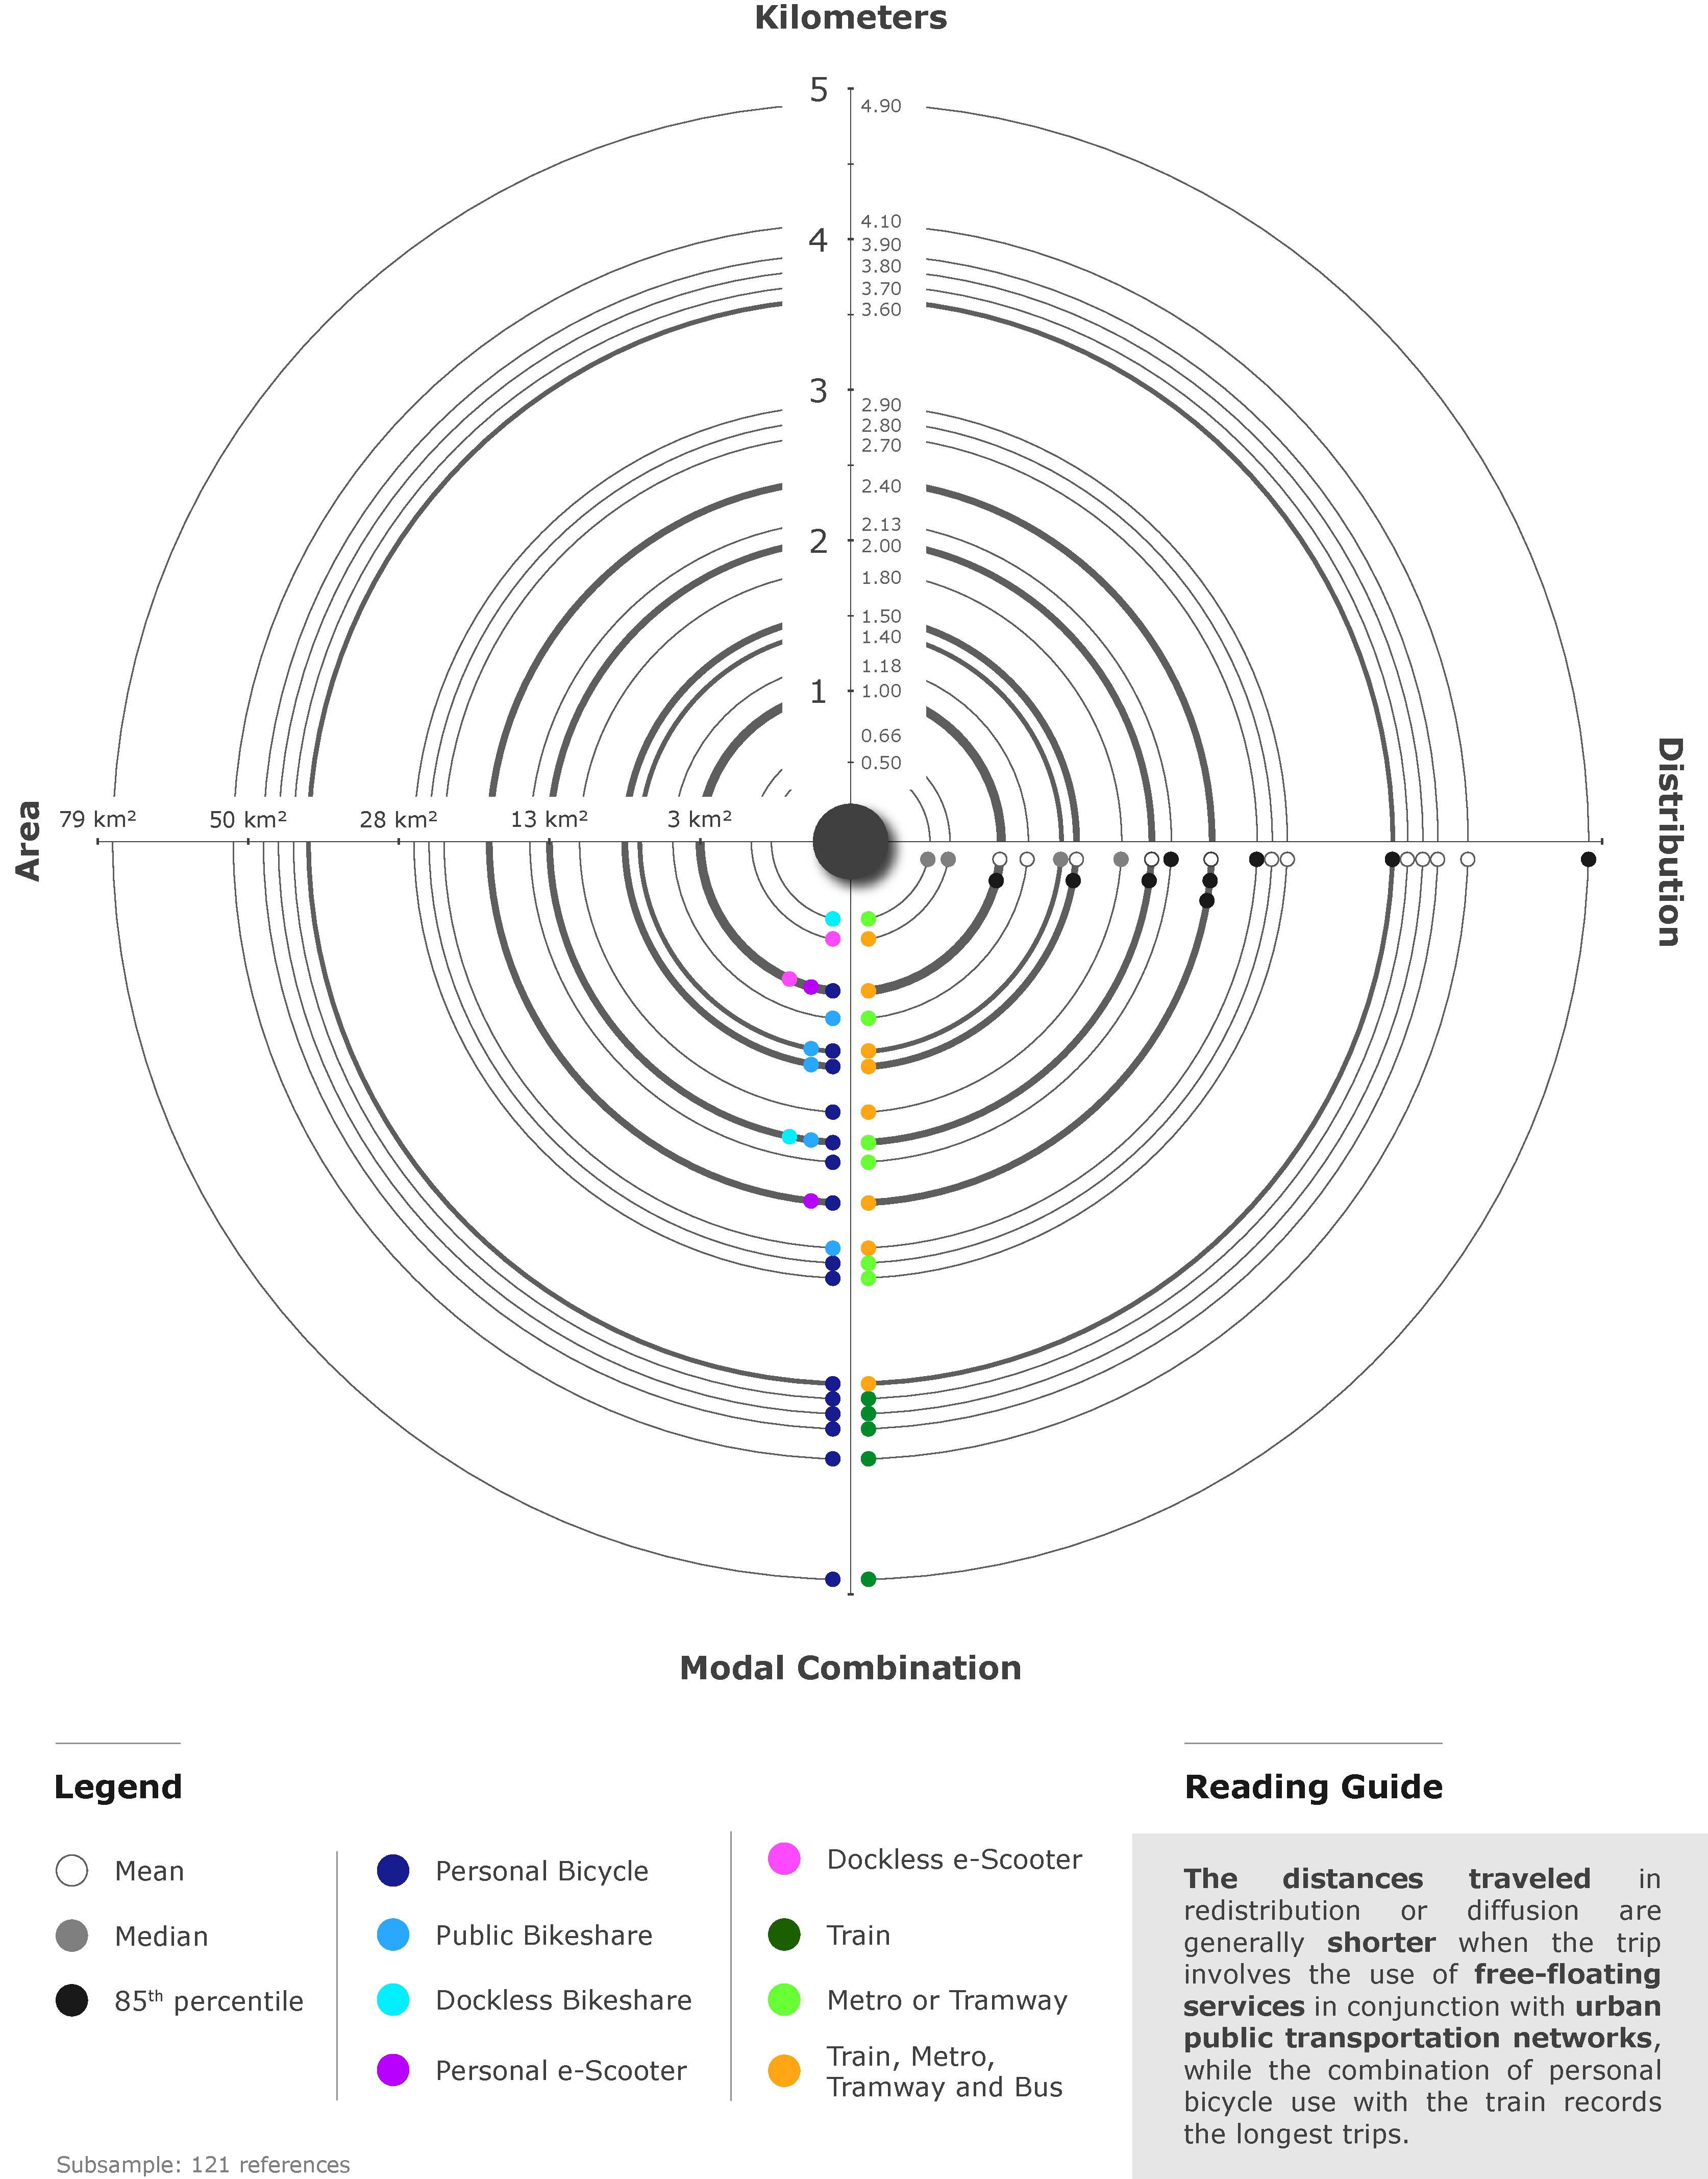
\includegraphics[width=1\columnwidth]{src/Figures/Chap-2/EN_RSL_Aires_influence.pdf}}
    \vspace{5pt}
    \begin{flushright}\scriptsize{
    Author: \textcolor{blue}{Dylan Moinse (2023)}
    }\end{flushright}
\end{figure}

% Distances time
Time-distance related to intermodality is a less explored aspect in the scientific literature, but a few studies provide important insights into the duration of trips combining light individual mobility and public transport. In Shanghai, \textcolor{blue}{\textcite[19]{lin_analysis_2019}}\index{Lin, Diao|pagebf}\index{Zhang, Yongping|pagebf}\index{Zhu, Ruoxin|pagebf}\index{Meng, Liqiu|pagebf} evaluate the average duration of a trip in \acrshort{DBS} to access a subway station as 8.2 minutes, equivalent to two kilometers. In Utrecht, trips by personal bike to and from public transport stations reveal distinct median durations: for access to the stations, the median duration is 10.1 minutes, corresponding to a distance of 1.8 kilometers, while for egress from the stations, it reaches 12.5 minutes, or a distance of 2.4 kilometers, according to \textcolor{blue}{\textcite[268]{krygsman_multimodal_2004}}\index{Krygsman, Stephan|pagebf}\index{Dijst, Martin|pagebf}\index{Arentze, Theo|pagebf}. In the Provence-Alpes-Côte d'Azur region, \textcolor{blue}{\textcite[186]{moinse_intermodal_2022}}\index{Moinse, Dylan|pagebf}\index{Goudeau, Matthieu|pagebf}\index{L'Hostis, Alain|pagebf}\index{Leysens, Thomas|pagebf} observe an average trip duration in \acrshort{PeS} of 10.6 minutes in combination with the train, equivalent to a distance of 2.4 kilometers. The use of \acrshort{PBS} in combination with the subway and bus presents an average travel time of 16 minutes, as shown in the case study on Taipei \textcolor{blue}{\autocite[49]{lu_improving_2018}}\index{Lu, Miaojia|pagebf}\index{Hsu, Shu Chien|pagebf}\index{Chen, Pi Cheng|pagebf}\index{Lee, Wan Yu|pagebf}, while this combination reaches a maximum value (95\textsuperscript{th} percentile) of 30 minutes in Nanjing \textcolor{blue}{\autocite[64]{ma_understanding_2018}}\index{Ma, Xinwei|pagebf}\index{Ji, Yanjie|pagebf}\index{Yang, Mingyuan|pagebf}\index{Jin, Yuchuan|pagebf}\index{Tan, Xu|pagebf}.%%Translated%%

% 2.3.5.4. Influence areas
\subsubsection*{Influence Areas
    \label{chap2:aires-influence}
    }

% <3km
The reviewed documentation is based on a defined study perimeter based on the distribution of spatial distances. In this regard, several academic studies have identified areas of influence with relatively limited reach, primarily focusing on public transport stops in urban areas. Thus, \textcolor{blue}{\textcite[5]{wang_interchange_2016}}\index{Wang, Zi-jia|pagebf}\index{Chen, Feng|pagebf}\index{Xu, Tian-kun|pagebf} observed that cycling distances in Beijing are mainly between 0.4 and 1.4 kilometers. According to the work of \textcolor{blue}{\textcite[11]{hu_examining_2022}}\index{Hu, Songhua|pagebf}\index{Chen, Mingyang|pagebf}\index{Jiang, Yuan|pagebf}\index{Sun, Wei|pagebf}\index{Xiong, Chenfeng|pagebf}, the relevant spatial distance for modeling the use of \acrshort{DBS} in Shanghai ranges from 1 to 1.5 kilometers, with suburban areas generally characterized by longer trips. This same influence perimeter is also adopted by \textcolor{blue}{\textcite[9]{jin_competition_2019}}\index{Jin, Haitao|pagebf}\index{Jin, Fengjun|pagebf}\index{Wang, Jiao'e|pagebf}\index{Sun, Wei|pagebf}\index{Dong, Libo|pagebf} and by \textcolor{blue}{\textcite[10]{fan_how_2019}}\index{Fan, Aihua|pagebf}\index{Chen, Xumei|pagebf}\index{Wan, Tao|pagebf} in the urban context of Beijing, suggesting an action radius of up to two kilometers for \acrshort{DBS}. In Shanghai, \textcolor{blue}{\textcite[185]{pan_intermodal_2010}}\index{Pan, Haixiao|pagebf}\index{Shen, Qing|pagebf}\index{Xue, Song|pagebf} determine an area ranging from 0.8 to 2.5 kilometers, emphasizing that the majority of bicycle and \acrshort{e-Bike} trips occur within distances less than 1.5 kilometers. According to \textcolor{blue}{\textcite[5]{ma_connecting_2022}}\index{Ma, Qingyu|pagebf}\index{Xin, Yanan|pagebf}\index{Yang, Hong|pagebf}\index{Xie, Kun|pagebf}, a perimeter between two and three kilometers was established to assess the reach of \acrshort{DESS} in Washington, D.C., with a similar approach observed in Beijing for \acrshort{DBS} \textcolor{blue}{\autocite[6]{ma_connecting_2022}}\index{Ma, Qingyu|pagebf}\index{Xin, Yanan|pagebf}\index{Yang, Hong|pagebf}\index{Xie, Kun|pagebf} as well as in Atlanta for cycling \textcolor{blue}{\autocite[57]{bearn_adaption_2018}}\index{Bearn, Cary|pagebf}\index{Mingus, Charlene|pagebf}\index{Watkins, Kari|pagebf}. It should be noted that the distance thresholds mentioned specifically relate to urban public transport networks, such as the subway. Therefore, the spatial configuration of these transport infrastructures, characterized by short distances between stations, can explain the small size of the measured influence areas.%%Translated%%

% >3km
From a radius of two to three kilometers, the considered geographical areas are more suitable for intermodal use of cycling combined with the train. Through an investigation in the Netherlands, \textcolor{blue}{\textcite[227]{keijer_how_2000}}\index{Keijer, Majanka|pagebf}\index{Rietveld, Piet|pagebf} and \textcolor{blue}{\textcite[73]{rietveld_accessibility_2000}}\index{Rietveld, Piet|pagebf} introduce a framework based on distance decay factors, thus justifying the establishment of an extended perimeter of 1 to 3.5 kilometers, beyond which the attraction to cycle usage tends to decrease. This observation is corroborated by the work of \textcolor{blue}{\textcite[281]{debrezion_modelling_2009}}\index{Debrezion, Ghebreegziabiher|pagebf}\index{Pels, Eric|pagebf}\index{Rietveld, Piet|pagebf}, which confirms that cycling is competitive for distances ranging from 1.1 to 4.2 kilometers to or from the station. Various scholarly works extend the influence area up to five kilometers, as evidenced by the use of \acrshort{DBS} in Shenzhen \textcolor{blue}{\autocite[6]{wu_measuring_2019}}\index{Wu, Xueying|pagebf}\index{Lu, Li|pagebf}\index{Lin, Yaoyu|pagebf}\index{Yang, Yiyang|pagebf}, or the combination of \acrshort{PBS} and cycling with the metro in Beijing \textcolor{blue}{\autocite[54]{zhao_bicycle-metro_2017}}\index{Zhao, Pengjun|pagebf}\index{Li, Shengxiao|pagebf}. The same impact zone is identified concerning the combination of cycling and the train, whether in Amboise \textcolor{blue}{\autocite[751]{midenet_modal_2018}}\index{Midenet, Sophie|pagebf}\index{Côme, Etienne|pagebf}\index{Papon, Francis|pagebf}, in Göteborg, Malmö, and Beijing \textcolor{blue}{\autocite[15]{hamidi_shaping_2020}}\index{Hamidi, Zahra|pagebf}\index{Zhao, Chunli|pagebf}, in El Monte \textcolor{blue}{\autocite[118]{cottrell_transforming_2007}}\index{Cottrell, Wayne~D.|pagebf}, or in Xi'an \textcolor{blue}{\autocite[172]{yang_bike-and-ride_2014}}\index{Yang, Liu|pagebf}\index{Chao, Li|pagebf}\index{Wang, Yuanqing|pagebf}. Going even further, \textcolor{blue}{\textcite[9]{kim_analysis_2021}}\index{Kim, Minjun|pagebf}\index{Cho, Gi-Hyoung|pagebf} support that trips combining \acrshort{PBS} and the metro in Seoul are frequent up to a distance of ten kilometers, thus highlighting the extended reach of these intermodal practices.%%Translated%%

% Temps
From a temporal perspective, part of the academic documentation has focused on determining the influence areas of public transport stations, taking the temporal variable into account. In this regard, \textcolor{blue}{\textcite[18, 21]{li_factors_2020}}\index{Li, Xuefeng|pagebf}\index{Du, Mingyang|pagebf}\index{Yang, Jingzong|pagebf} highlighted that \acrshort{DBS} trips lasting less than seven minutes predominate, especially during morning peak periods on weekdays, although some regions of Shenzhen, including its city center, show a majority of trips exceeding fifteen minutes. According to \textcolor{blue}{\textcite[128]{liu_understanding_2020}}\index{Liu, Yang|pagebf}\index{Ji, Yanjie|pagebf}\index{Feng, Tao|pagebf}\index{Timmermans, Harry~J.~P.|pagebf}, a biking duration of more than ten minutes reduces its use in combination with the metro in Nanjing. This duration is set at twelve minutes for the joint use of \acrshort{PBS} and the rail network in Boston, Chicago, Washington~D.C., and New York City \textcolor{blue}{\autocite[9]{kong_deciphering_2020}}\index{Kong, Hui|pagebf}\index{Jin, Scarlett~T.|pagebf}\index{Sui, Daniel~Z.|pagebf}, and extends to fifteen minutes for \acrshort{PBS} combined with the train in Osaka \textcolor{blue}{\autocite[3415]{tomita_demand_2017}}\index{Tomita, Yasuo|pagebf}\index{Nakayama, Akihiko|pagebf}. \textcolor{blue}{\textcite[5]{yang_empirical_2016}}\index{Yang, Min|pagebf}\index{Liu, Xinlu|pagebf}\index{Wang, Wei|pagebf}\index{Li, Zhibin|pagebf}\index{Zhao, Jingyao|pagebf} define a temporal perimeter of twenty minutes for the use of \acrshort{PBS} in relation to the metro network in Nanjing. Finally, \textcolor{blue}{\textcite[1696]{cheng_evaluating_2012}}\index{Cheng, Yung-Hsiang|pagebf}\index{Liu, Kuo-Chu|pagebf} adopt a more systemic approach by simultaneously measuring travel times for both feeder and egress trips, observing that the majority of cyclists using the metro in Kaohsiung make round trips of less than thirty minutes.%%Translated%%

% 2.3.5.5. Variability of Distances and Detours
\subsubsection*{Variability of Distances
    \label{chap2:variabilite-distances}
    }

    % Facteurs
The evaluation of the actual distances traveled by intermodal travelers, particularly for the \Commas{first and last miles,} is closely linked to the route choices made. These trips, taken by cyclists, are influenced by a variety of factors related to the urban environment, temporal context, as well as behaviors, habits, and mobility experiences. According to \textcolor{blue}{\textcite[15]{tzouras_describing_2023}}\index{Tzouras, Panagiotis|pagebf}\index{Mitropoulos, Lambros|pagebf}\index{Koliou, Katerina|pagebf}\index{Stavropoulou, Eirini|pagebf}\index{Karolemeas, Christos|pagebf}\index{Antoniou, Eleni|pagebf}\index{Karaloulis, Antonis|pagebf}\index{Mitropoulos, Konstantinos|pagebf}\index{Vlahogianni, Eleni~I.|pagebf}\index{Kepaptsoglou, Konstantinos|pagebf}, users of \acrshort{PeS} in Athens select their routes considering perceived safety and minimum distance, aiming to balance the required physical effort and the physical and psychological barriers to avoid. \textcolor{blue}{\textcite[621]{krizek_detailed_2007}}\index{Krizek, Kevin~J.|pagebf}\index{El-Geneidy, Ahmed~M.|pagebf}\index{Thompson, Kristin|pagebf} observe that the measured distances are also determined by the purpose of the trip: bike and tram journeys associated with shopping and work are shorter, while those related to leisure are longer, in Minneapolis. The environmental and temporal context also has a notable impact on the distances traveled. In this regard, \textcolor{blue}{\textcite[619]{krizek_detailed_2007}}\index{Krizek, Kevin~J.|pagebf}\index{El-Geneidy, Ahmed~M.|pagebf}\index{Thompson, Kristin|pagebf} show that cyclists are willing to extend their journey by up to 67\% to reach a high-quality bike path. \textcolor{blue}{\textcite[8]{adnan_last-mile_2019}}\index{Adnan, Muhammad|pagebf}\index{Altaf, Shahbaz|pagebf}\index{Bellemans, Tom|pagebf}\index{Yasar, Ansar-ul-Haque|pagebf}\index{Shakshuki, Elhadi~M.|pagebf} demonstrated that \acrshort{PBS} users in medium-sized cities in Belgium are sensitive to weather factors such as temperature and rainfall, influencing not only their routes but also their modal choices. \textcolor{blue}{\textcite[3110]{cho_estimation_2022}}\index{Cho, Shin-Hyung|pagebf}\index{Shin, DongHwa|pagebf} found that \acrshort{PBS} users in Seoul are more sensitive to distance in the evening compared to other times of the day. In Nanjing, \textcolor{blue}{\textcite[11]{li_operating_2019}}\index{Li, Yuan|pagebf}\index{Zhu, Zhenjun|pagebf}\index{Guo, Xiucheng|pagebf} revealed that the reach of \acrshort{DBS} varies depending on the day of the week and the type of metro station. These findings are consistent with those of \textcolor{blue}{\textcite[105]{flamm_public_2014}}\index{Flamm, Bradley~J.|pagebf}\index{Rivasplata, Charles~R.|pagebf}, who noted that the distances traveled by cyclists in Philadelphia and San Francisco depend on the type of public transport and the topography. Additionally, trains cover longer distances compared to conventional and express bus services, representing a more significant variable than socio-demographic factors, which have a moderate impact on distance in several U.S. cities \textcolor{blue}{\autocite[23-24]{hochmair_assessment_2015}}\index{Hochmair, Hartwig~H.|pagebf}. Finally, metro stations located on the outskirts of Shanghai have significantly larger catchment areas than those in the city center \textcolor{blue}{\autocite[8]{yu_policy_2021}}\index{Yu, Qing|pagebf}\index{Li, Weifeng|pagebf}\index{Yang, Dongyuan|pagebf}\index{Xie, Yingkun|pagebf}. This variety of factors affecting the relationship with distance illustrates how cyclists do not always prioritize the shortest route, revealing strategies aimed at balancing spatial-temporal optimization with comfort.%%Translated%%

% Détours
Several research studies highlight the practice of detours by intermodal travelers, who cover longer distances due to multiple factors. According to \textcolor{blue}{\textcite[102]{kampen_understanding_2020}}\index{Kampen, Jullian van|pagebf}\index{Jayaraj, Manoj Ashvin|pagebf}\index{Pauwels, Eric|pagebf}\index{Mei, Rob van der|pagebf}\index{Dugundji, Elenna~R.|pagebf}, 42\% of cyclists are inclined to head towards more distant stations rather than the nearest station, favoring those with better connectivity, in the regions of North-Holland, South-Holland, Flevoland, and Utrecht. On the one hand, \textcolor{blue}{\textcite[18]{jonkeren_bicycle-train_2021}}\index{Jonkeren, Olaf|pagebf}\index{Kager, Roland|pagebf}\index{Harms, Lucas|pagebf}\index{te Brömmelstroet, Marco|pagebf} emphasize the goal of bypassing transfer breaks by favoring stations with better facilities, such as those in Utrecht, Rotterdam, and Eindhoven. On the other hand, this preference also extends to metro stations offering bicycle parking facilities, as shown in the case study conducted by \textcolor{blue}{\textcite[342]{kampen_bicycle_2021}}\index{Kampen, Jullian van|pagebf}\index{Pauwels, Eric|pagebf}\index{Mei, Rob van der|pagebf}\index{Dugundji, Elenna~R.|pagebf} in Amsterdam. In Shanghai, \textcolor{blue}{\textcite[7]{li_exploring_2021}}\index{Li, Wenxiang|pagebf}\index{Chen, Shawen|pagebf}\index{Dong, Jieshuang|pagebf}\index{Wu, Jingxian|pagebf} reveal that the busiest public transport stations attract \acrshort{DBS} passengers from farther away. \textcolor{blue}{\textcite[143]{kampen_understanding_2021}}\index{Kampen, Jullian van|pagebf}\index{Jayaraj, Manoj Ashvin|pagebf}\index{Pauwels, Eric|pagebf}\index{Mei, Rob van der|pagebf}\index{Dugundji, Elenna~R.|pagebf} add that cyclists with a net monthly income of less than~\euro2,500 and aged over 39 are more likely to go to the second nearest station to their departure point. The role of factors influencing the actual distances traveled reflects the importance of policies and strategies aimed at guiding people's mobility to make alternative mobility systems more attractive compared to car use.%%Translated%%

% 2.3.6. Resultats : management de la demande
\subsection{Mobility Demand Management
    \label{chap2:gestion-demande-mobilite}
    }

    % Introduction
Mobility demand management, encompassing all strategies and policies aimed at influencing individuals' travel choices, is at the core of 61 scientific studies addressing \acrshort{M-TOD}. Our analysis will begin by examining the role of the service level offered by public transport systems and the importance of implementing integrated pricing. We will then discuss the contribution of shared mobility services, as well as the role of bus networks in transit-oriented neighborhoods. Finally, this section will address traffic and parking management.%%Translated%%

% 2.3.6.1. Fréquence et temps d'attente
\subsubsection*{Mass Transit Service Level
    \label{chap2:niveau-service}
    }

    % Frequency of public transport
A regular and punctual rail service seems to favor the use of bicycles in intermodal travel. This observation has been noted for trains in the Randstad South \textcolor{blue}{\autocite[45]{la_paix_puello_modelling_2015}}\index{La Paix Puello, Lissy|pagebf}\index{Geurs, Karst~T.|pagebf}, Rotterdam \textcolor{blue}{\autocite[5]{montes_shared_2023}}\index{Montes, Alejandro|pagebf}\index{Geržinic, Nejc|pagebf}\index{Veeneman, Wijnand|pagebf}\index{Oort, Niels van|pagebf}\index{Hoogendoorn, Serge|pagebf}, Turin \textcolor{blue}{\autocite[12]{staricco_implementing_2020}}\index{Staricco, Luca|pagebf}\index{Vitale Brovarone, Elisabetta|pagebf}, and Shanghai for the \acrshort{DBS} in combination with the metro \textcolor{blue}{\autocite[24]{lin_analysis_2019}}\index{Lin, Diao|pagebf}\index{Zhang, Yongping|pagebf}\index{Zhu, Ruoxin|pagebf}\index{Meng, Liqiu|pagebf}. In Melbourne, \textcolor{blue}{\textcite[401]{weliwitiya_bicycle_2019}}\index{Weliwitiya, Hesara|pagebf}\index{Rose, Geoff|pagebf}\index{Johnson, Marilyn|pagebf} highlighted a positive correlation between the frequency of rail lines, particularly during the morning peak hours, and the use of bicycles as a feeder mode. The authors found that an increase of one unit in frequency led to an increase of 1.03 in the number of intermodal cyclists. In Poznań, \textcolor{blue}{\textcite[199]{radzimski_exploring_2021}}\index{Radzimski, Adam|pagebf}\index{Dzięcielski, Michał|pagebf} demonstrated a positive correlation between the frequency of tram lines and the number of \acrshort{PBS} trips for short distances, up to 1.5 kilometers, and for medium distances, between 1.5 and 3 kilometers. However, this relationship was not observed for trips exceeding 3 kilometers. However, \textcolor{blue}{\textcite[301]{kuijk_preferences_2022}}\index{Mil, Joeri~F.P. van|pagebf}\index{Leferink, Tessa~S.|pagebf}\index{Annema, Jan Anne|pagebf}\index{Oort, Niels van|pagebf}\index{Kuijk, Roy~J. van|pagebf}\index{Almeida Correia, Gonçalo Homem de|pagebf}\index{Oort, Niels van|pagebf}\index{Arem, Bart van|pagebf} did not identify any significant parameters concerning the frequency and speed of trams related to the use of \acrshort{PBS} in Utrecht. Moreover, the results of studies by \textcolor{blue}{\textcite[41]{nielsen_bikeability_2018}}\index{Nielsen, Thomas Alexander Sick|pagebf}\index{Skov-Petersen, Hans|pagebf} suggest that the frequency of rail services might decrease the likelihood of using bicycles in Denmark.%%Translated%%

% Station density
Beyond the frequency of public transport services, the commercial speed of these collective modes, intrinsically linked to travel time, proves to be a key factor in modal choice favoring the bicycle. This trend contrasts with the minor role attributed to the punctuality and safety of rail services in Eindhoven \textcolor{blue}{\autocite[727]{waerden_relation_2018}}\index{Waerden, Peter|pagebf}\index{Waerden, Jaap|pagebf}. The speed of public transport journeys is largely influenced by the density of stations, which has a significant impact on the demand for bike transfers. Indeed, very close train stations tend to reduce the likelihood of opting for this mode of transport in Denmark \textcolor{blue}{\autocite[41]{nielsen_bikeability_2018}}\index{Nielsen, Thomas Alexander Sick|pagebf}\index{Skov-Petersen, Hans|pagebf}. In contrast, the density of metro stations positively affects the use of \acrshort{PBS} in Nanjing \textcolor{blue}{\autocite[17]{ji_exploring_2018}}\index{Ji, Yanjie|pagebf}\index{Ma, Xinwei|pagebf}\index{Yang, Mingyuan|pagebf}\index{Jin, Yuchuan|pagebf}\index{Gao, Liangpeng|pagebf}. Exploring the combination of \acrshort{DBS} and metro in Beijing, \textcolor{blue}{\textcite[10]{guo_exploring_2023}}\index{Guo, Dongbo|pagebf}\index{Yao, Enjian|pagebf}\index{Liu, Shasha|pagebf}\index{Chen, Rongsheng|pagebf}\index{Hong, Junyi|pagebf}\index{Zhang, Junyi|pagebf} found that waiting time has a much more negative impact than travel time itself—users are willing to pay~\euro13.6 (CNY~105) to save an hour of waiting time, compared to~\euro2 (CNY~15) for an hour of \acrshort{DBS}—highlighting the need to establish efficient connections within the public transport system to address the aversion to transfer times.%%Translated%%

% 2.3.6.2. MaaS and pricing
\needspace{1\baselineskip} % Reserve space
\subsubsection*{Integrated pricing
    \label{chap2:tarification_integree}
    }

% MaaS
To promote integration and encourage intermodal practices, the scientific literature recommends simplifying the connections between different mobility systems by promoting the use of integrated transport cards \textcolor{blue}{\autocite[172]{yang_bike-and-ride_2014}}\index{Yang, Liu|pagebf}\index{Chao, Li|pagebf}\index{Wang, Yuanqing|pagebf}, the most popular option among passengers \textcolor{blue}{\autocite[10]{yang_empirical_2016}}\index{Yang, Min|pagebf}\index{Liu, Xinlu|pagebf}\index{Wang, Wei|pagebf}\index{Li, Zhibin|pagebf}\index{Zhao, Jingyao|pagebf}. One of the main levers identified is shared light individual mobility and the implementation of a multimodal platform like \acrshort{MaaS}, offering the possibility of pooling or even unifying online payments \textcolor{blue}{\autocite[5]{fearnley_patterns_2020}}\index{Fearnley, Nils|pagebf}\index{Johnsson, Espen|pagebf}\index{Berge, Siri Hegna|pagebf}. In Nanjing, a lack of information about bike rental facilities has been noted, despite clear interest in the service, highlighting the importance of \acrshort{MaaS} \textcolor{blue}{\autocite[136]{chen_determinants_2012}}\index{Chen, Lijun|pagebf}\index{Pel, Adam~J.|pagebf}\index{Chen, Xuewu|pagebf}\index{Sparing, Daniel|pagebf}\index{Hansen, Ingo~A.|pagebf}. According to \textcolor{blue}{\textcite[67]{ma_understanding_2018}}\index{Ma, Xinwei|pagebf}\index{Ji, Yanjie|pagebf}\index{Yang, Mingyuan|pagebf}\index{Jin, Yuchuan|pagebf}\index{Tan, Xu|pagebf}, integrated platforms should include a loyalty program to prioritize frequent \acrshort{PBS} and public transport users by reserving bike-sharing locations for these users. However, \textcolor{blue}{\textcite[12]{fan_how_2019}}\index{Fan, Aihua|pagebf}\index{Chen, Xumei|pagebf}\index{Wan, Tao|pagebf} highlight barriers to using the \acrshort{DBS} or a \acrshort{MaaS} platform in Beijing, such as the need to install a mobile app, provide personal information for registration, and pay a large deposit, while pricing remains the main factor influencing the choice of \acrshort{DBS}.%%Translated%%

% Bike-sharing and shared micromobility pricing
The costs of bike-sharing and shared micromobility are often deemed prohibitive, discouraging their use for first- and last-mile trips, and even more so for long-distance trips \textcolor{blue}{\autocite[5]{montes_shared_2023}}\index{Montes, Alejandro|pagebf}\index{Geržinic, Nejc|pagebf}\index{Veeneman, Wijnand|pagebf}\index{Oort, Niels van|pagebf}\index{Hoogendoorn, Serge|pagebf}. In Nanjing, young workers choose \acrshort{PBS} for economic reasons, raising questions about pricing strategies that do not encourage the long-term use of these sustainable mobility practices. In this regard, the costs of a single trip and a subscription to the service have a significant impact on the choice of \acrshort{DBS} to access the metro network \textcolor{blue}{\autocite[17]{zhong_layout_2021}}\index{Zhong, Hongming|pagebf}\index{Liu, Zijian|pagebf}\index{Chen, Jun|pagebf}\index{Hao, Jun|pagebf}\index{Wang, Wei|pagebf}. In Beijing, travelers using \acrshort{DBS} spend almost as much on short trips using this service as they do on public transport \textcolor{blue}{\autocite[12]{fan_how_2019}}\index{Fan, Aihua|pagebf}\index{Chen, Xumei|pagebf}\index{Wan, Tao|pagebf}. Several solutions emerge from these findings. In Nanjing, a free two-hour bike rental policy, as an effective promotional strategy for 57\% of travelers, has been identified by \textcolor{blue}{\textcite[135]{chen_determinants_2012}}\index{Chen, Lijun|pagebf}\index{Pel, Adam~J.|pagebf}\index{Chen, Xuewu|pagebf}\index{Sparing, Daniel|pagebf}\index{Hansen, Ingo~A.|pagebf}. In Washington D.C. and Los Angeles, pricing incentives favoring the use of \acrshort{DESS} with the metro are being evaluated, including price reductions when a~\euro2.8 (\$3) credit is applied to scooter fares \textcolor{blue}{\autocite[11]{yan_evaluating_2023}}\index{Yan, Xiang|pagebf}\index{Zhao, Xilei|pagebf}\index{Broaddus, Andrea|pagebf}\index{Johnson, Joshua|pagebf}\index{Srinivasan, Sivaramakrishnan|pagebf}. In Boston and Worcester, the impact of different pricing schemes is analyzed, revealing that a combination of a fixed fare and distance-based fare has the least impact on the demand for bike and train combinations \textcolor{blue}{\autocite[16]{fournier_continuous_2021}}\index{Fournier, Nicholas|pagebf}\index{Christofa, Eleni|pagebf}\index{Gonzales, Eric~J.|pagebf}, while in Oslo, the price per minute is an important factor in promoting the use of \acrshort{DESS} with public transport \textcolor{blue}{\autocite[5]{fearnley_patterns_2020}}\index{Fearnley, Nils|pagebf}\index{Johnsson, Espen|pagebf}\index{Berge, Siri Hegna|pagebf}. A social pricing scheme based on income is considered effective for \acrshort{DBS} and \acrshort{DESS} in Seattle to alleviate financial barriers \textcolor{blue}{\autocite[975-977]{beale_integrating_2023}}\index{Beale, Kirsten|pagebf}\index{Kapatsila, Bogdan|pagebf}\index{Grisé, Emily|pagebf}.%%Translated%%

% Pricing for public transport and bike parking
Finally, monetary cost also affects the use of public transport as well as bike and micromobility parking. The free access to rail services targeted at students in the Netherlands attracts more intermodal cyclists at the expense of automobiles \textcolor{blue}{\autocite[360]{givoni_access_2007}}\index{Givoni, Moshe|pagebf}\index{Rietveld, Piet|pagebf}. A significant aversion to bike parking fees is observed among Dutch students \textcolor{blue}{\autocite[667]{mil_insights_2020}}\index{Mil, Joeri~F.P. van|pagebf}\index{Leferink, Tessa~S.|pagebf}\index{Annema, Jan Anne|pagebf}\index{Oort, Niels van|pagebf}. However, \textcolor{blue}{\textcite[10]{molin_bicycle_2015}}\index{Molin, Eric|pagebf}\index{Maat, Kees|pagebf} indicate that free bike parking does not influence the use of bikes for intermodality in the Netherlands, and on the contrary, 65\% of the cyclists surveyed prefer the scenario based on secure, paid parking with an optimal price of 1.50\euro. Similarly, \textcolor{blue}{\textcite[5]{liu_mode_2022}}\index{Liu, Lumei|pagebf}\index{Kong, Hui|pagebf}\index{Liu, Tianliang|pagebf}\index{Ma, Xiaolei|pagebf} find that the cost of the trip has little impact on the choice between the bus or \acrshort{DBS} when transferring with the metro in Beijing, suggesting that the quality of bike-sharing infrastructure is a more important factor to consider.%%Translated%%

% 2.3.6.3. Shared Bike and micromobility Services
\subsubsection*{Transfer Services
    \label{chap2:services-transfert}
    }

% Presence of bike-sharing
The availability of shared mobility systems, such as \acrshort{PBS}, \acrshort{DBS}, or \acrshort{DESS}, is a fundamental element for integrating bicycles with public transport \textcolor{blue}{\autocite[11-12]{wu_measuring_2019}}\index{Wu, Xueying|pagebf}\index{Lu, Li|pagebf}\index{Lin, Yaoyu|pagebf}\index{Yang, Yiyang|pagebf}. Thus, the incorporation of these mobility services within the urban \acrshort{TOD} strategy is recommended to increase the use and overall efficiency of the mobility system \textcolor{blue}{\autocite[16]{tamakloe_determinants_2021}}\index{Tamakloe, Reuben|pagebf}\index{Hong, Jungyeol|pagebf}\index{Tak, Jihoon|pagebf}. The availability of bikes and micromobility options in bike-sharing systems close to transport hubs not only increases the probability of their use as connection modes \textcolor{blue}{\autocite[25]{guo_dockless_2021}}\index{Guo, Yuanyuan|pagebf}\index{Yang, Linchuan|pagebf}\index{Lu, Yi|pagebf}\index{Zhao, Rui|pagebf}, but these systems also contribute to promoting more efficient intermodal travel practices, reducing the need for a second bike \textcolor{blue}{\autocite[10]{jonkeren_bicycle_2021}}\index{Jonkeren, Olaf|pagebf}\index{Kager, Roland|pagebf}. In Shanghai, \textcolor{blue}{\textcite[186]{pan_intermodal_2010}}\index{Pan, Haixiao|pagebf}\index{Shen, Qing|pagebf}\index{Xue, Song|pagebf} identified a strong willingness expressed by study participants to use bike rental systems near metro stations. Based on the observation that intermodal travelers have a high degree of trip planning and adapt their behavior according to mobility offerings and constraints related to transport and bike parking, \textcolor{blue}{\textcite[196]{sherwin_practices_2011}}\index{Sherwin, Henrietta|pagebf}\index{Parkhurst, Graham|pagebf}\index{Robbins, Derek|pagebf}\index{Walker, Ian|pagebf} justify the establishment of a nationwide organized bike rental system, similar to what is practiced by Dutch and German railway operators.%%Translated%%

% Management and Redistribution of Shared Bike and micromobility Services
The implementation of a shared light individual mobility system requires efficient management and optimal fleet distribution. The work of \textcolor{blue}{\textcite[197]{radzimski_exploring_2021}}\index{Radzimski, Adam|pagebf}\index{Dzięcielski, Michał|pagebf} demonstrates that structuring a \acrshort{PBS} system, organized in the form of dockless bikes with dedicated stations, attracts more users in combination with trams compared to \acrshort{DBS}. Therefore, it is recommended to improve the allocation of \acrshort{DBS} by more efficiently redistributing bikes towards green spaces, commercial and industrial areas, as well as residential neighborhoods in Beijing \textcolor{blue}{\autocite[12]{liu_temporal_2022}}\index{Liu, Siyang|pagebf}\index{Zhang, Xiaodong|pagebf}\index{Zhou, Chenjing|pagebf}\index{Rong, Jian|pagebf}\index{Bian, Yang|pagebf}. Given the capacity limitations of dockless sharing systems during usage peaks, as observed for \acrshort{DESS} in Columbus \textcolor{blue}{\autocite[9]{liu_measuring_2022}}\index{Liu, Luyu|pagebf}\index{Miller, Harvey~J.|pagebf}, \textcolor{blue}{\textcite[69, 95]{nat_bicycle_2018}}\index{Nat, Johanna Debóra van der|pagebf} suggests an alternative bike-sharing model. This model relies on a combination of rental and sufficient availability of shared bikes to ensure their accessibility and maximize parking space savings in Amsterdam.%%Translated%%

% Embarkation / Carrying in Public Transport
The establishment of efficient connections between public transport systems and light individual mobility is also reflected in the ease of carrying bikes and micromobility devices aboard public transport modes. Combined with the implementation of an effective bike-sharing and micromobility service system and parking facilities, the boarding of light individual mobility in public transport vehicles stimulates intermodal practices in Portland \textcolor{blue}{\autocite[93]{singleton_exploring_2014}}\index{Singleton, Patrick~A.|pagebf}\index{Clifton, Kelly~J.|pagebf}. In Copenhagen, \textcolor{blue}{\textcite[19]{halldorsdottir_home-end_2017}}\index{Halldórsdóttir, Katrín|pagebf}\index{Nielsen, Otto Anker|pagebf}\index{Prato, Carlo Giacomo|pagebf} demonstrate that the ability to transport a bike for free on the train increases the intermodal use of bicycles. Moreover, managing bike and micromobility interconnections should be considered in relation to bus services, as a substitution effect between \acrshort{PBS} and \acrshort{DBS} with the bus is observed in Nanjing \textcolor{blue}{\autocite[12]{chen_what_2022}}\index{Chen, Wendong|pagebf}\index{Chen, Xuewu|pagebf}\index{Chen, Jingxu|pagebf}\index{Cheng, Long|pagebf}.%%Translated%%

% Bus Service
\subsubsection*{Bus Service
    \label{chap2:desserte-bus}
    }

% Modal Substitution
Given the modal substitution effect between light individual mobility and buses, it appears that the density of bus stops in the area of influence of major public transport stations is inversely proportional to the use of these modes of transport. For example, in Beijing, bus services substitute for the use of bicycles, \acrshort{PBS} \textcolor{blue}{\autocite[55]{zhao_bicycle-metro_2017}}\index{Zhao, Pengjun|pagebf}\index{Li, Shengxiao|pagebf} and \acrshort{DBS} \textcolor{blue}{\autocite[16]{wang_spatiotemporal_2020}}\index{Wang, Zi-jia|pagebf}. \textcolor{blue}{\textcite[10]{li_exploring_2021}}\index{Li, Wenxiang|pagebf}\index{Chen, Shawen|pagebf}\index{Dong, Jieshuang|pagebf}\index{Wu, Jingxian|pagebf} observe that the density of bus stops decreases gradually as the transfer distance increases, providing a comparative advantage to \acrshort{DBS} when this distance exceeds a certain threshold in Shanghai. Similarly, \textcolor{blue}{\textcite[20]{luan_better_2020}}\index{Luan, Xin|pagebf}\index{Cheng, Lin|pagebf}\index{Song, Yan|pagebf}\index{Zhao, Jinbao|pagebf} find that residents of Nanjing tend to abandon the bus in favor of cycling, which could indicate dissatisfaction with existing bus services.%%Translated%%

% Absence of Modal Substitution
\textsl{A contrario}, a greater portion of studies seems to indicate an absence of modal substitution, revealing, on the contrary, that bus connections have a positive impact on the use of \acrshort{PBS} in combination with the train in Washington~D.C. \textcolor{blue}{\autocite[7-8]{ma_bicycle_2015}}\index{Ma, Ting|pagebf}\index{Liu, Chao|pagebf}\index{Erdoğan, Sevgi|pagebf} and \acrshort{DBS} with the metro in Shenzhen \textcolor{blue}{\autocite[12]{guo_built_2020}}\index{Guo, Yuanyuan|pagebf}\index{He, Sylvia~Y.|pagebf}. According to \textcolor{blue}{\textcite[20]{arbis_analysis_2016}}\index{Arbis, David|pagebf}\index{Hossein Rashidi, Taha|pagebf}\index{Dixit, Vinayak~V.|pagebf}\index{Vandebona, Upali|pagebf}, the presence of a bus stop near the stations is a predictive indicator of higher levels of bicycle parking usage in New South Wales. However, these reported conclusions may involve a misinterpretation of the data. Indeed, the observed correlation between the presence of bus stops and the increased use of bike-sharing could simply signal a better quality of service at the concerned stations, rather than establishing a direct cause-and-effect relationship. Furthermore, it is possible that these stations are located in areas where the development of bus stops coincides with policies aimed at reducing car space. While the mobility demand management aspect focuses on incentive measures—this section mainly addresses this dimension from the perspective of the level of service of collective modes, pricing, interconnection management, and bus service—competition with the automobile should not be overlooked, integrating a perspective on coercive policies. This approach should be considered to evaluate demand management strategies and their potential impact on promoting an alternative mobility system while reducing reliance on cars.%%Translated%%

% 2.3.6.5. Car
\needspace{1\baselineskip} % Réserve de l'espace
\subsubsection*{Moderation of Competitive Car Use
    \label{chap2:moderation-automobile}
    }

% Parking Reduction
In the context of urban development focused on the integration of public transport and light individual mobility, it is essential to consider the place of the car and highlight the importance of proactive policies to adapt public and private spaces to regulate traffic and motorized parking. A positive correlation is established between the increase in the motorization rate in an area and the increased use of cars to access stations in the Netherlands, with the car surpassing other modes of transfer starting from 0.60 cars per person for trips exceeding ten kilometers \textcolor{blue}{\autocite[281]{debrezion_modelling_2009}}\index{Debrezion, Ghebreegziabiher|pagebf}\index{Pels, Eric|pagebf}\index{Rietveld, Piet|pagebf}. In Provence-Alpes-Côte d'Azur, \textcolor{blue}{\autocite[190]{moinse_intermodal_2022}}\index{Moinse, Dylan|pagebf}\index{Goudeau, Matthieu|pagebf}\index{L'Hostis, Alain|pagebf}\index{Leysens, Thomas|pagebf} found that an intermodal trip takes a quarter more time than an equivalent car trip, excluding urban congestion and parking time, indicating the need for coercive measures if the competitiveness of cycling and \acrshort{PeS} with the train is to be increased.%%Translated%%

% Parking Recommendations
In Copenhagen, \textcolor{blue}{\textcite[18]{halldorsdottir_home-end_2017}}\index{Halldórsdóttir, Katrín|pagebf}\index{Nielsen, Otto Anker|pagebf}\index{Prato, Carlo Giacomo|pagebf} observed that the availability of car parking influences the choice of transfer modes to access stations. An increase of one hundred parking spaces around a station, typically equipped with 1,700 spaces, is linked to a 4\% decrease in walking and cycling usage, revealing a conflict between \acrfull{PnR} and \gls{active modes} in Toronto and Hamilton \textcolor{blue}{\autocite[2172-2173]{chan_factors_2020}}\index{Chan, Kevin|pagebf}\index{Farber, Steven|pagebf}. Furthermore, the saturation of parking lots around stations, and even more so at the destination, increases the likelihood of adopting active modes in the United States \textcolor{blue}{\autocite[4270]{bopp_examining_2015}}\index{Bopp, Melissa|pagebf}\index{Gayah, Vikash~V.|pagebf}\index{Campbell, Matthew~E.|pagebf}. Concerning egress from metro stations, it has been observed that the availability of parking spaces for motorcycles negatively influences passengers' intention to use \acrshort{PBS} in Kaohsiung \textcolor{blue}{\autocite[28]{cheng_expanding_2018}}\index{Cheng, Yung-Hsiang|pagebf}\index{Li, Yi-Chun|pagebf}. Therefore, it is suggested to strengthen regulations on the parking of motor vehicles around highly frequented stations to improve transportation demand management and enhance the competitiveness of combined cycling and metro in Xi'an \textcolor{blue}{\autocite[7]{zhu_improved_2021}}\index{Zhu, Zhenjun|pagebf}\index{He, Yudong|pagebf}\index{Guo, Xiucheng|pagebf}\index{Zhang, Yibang|pagebf}\index{Chen, Junlan|pagebf}. However, \textcolor{blue}{\textcite[401]{weliwitiya_bicycle_2019}}\index{Weliwitiya, Hesara|pagebf}\index{Rose, Geoff|pagebf}\index{Johnson, Marilyn|pagebf} warn against focusing solely on the car parking planned around stations without considering other types of parking, such as nearby streets or garages, which account for 72\% of the recorded parking for users arriving by car at the stations in Melbourne.%%Translated%%

% Parking Pricing
Beyond controlling access to parking, it has been shown that the introduction of BART in San Francisco led to an increase in parking fees around stations, which were previously free, thus encouraging bicycle usage \textcolor{blue}{\autocite[94]{cervero_bike-and-ride_2013}}\index{Cervero, Robert|pagebf}\index{Caldwell, Benjamin|pagebf}\index{Cuellar, Jesus|pagebf}. Several studies recommend better control of access to station parking through a pricing strategy inversely proportional to the transfer distance, as a lever for a powerful modal shift \textcolor{blue}{\autocite[751]{midenet_modal_2018}}\index{Midenet, Sophie|pagebf}\index{Côme, Etienne|pagebf}\index{Papon, Francis|pagebf}. In addition to car parking, \textcolor{blue}{\textcite[2737]{papon_evaluation_2017}}\index{Papon, Francis|pagebf}\index{Beauvais, Jean-Marie|pagebf}\index{Midenet, Sophie|pagebf}\index{Côme, Etienne|pagebf}\index{Polombo, Nadine|pagebf}\index{Abours, Sylvie|pagebf}\index{Belton-Chevallier, Leslie|pagebf}\index{Soulas, Claude|pagebf} conducted a socio-economic analysis showing that doubling the price of fuel would result in a 7\% increase in the modal share of cycling to stations.%%Translated%%

% 2.3.7. Results: Socio-demographic Profiles
\needspace{1\baselineskip} % Reserve space
\subsection{Socio-demographic Characteristics of Users
    \label{chap2:sociodemographie-usagers}
    }

    % Introduction
The revisited \acrshort{M-TOD} model, like any urban development strategy, must demonstrate its ability to promote inclusive accessibility. This means that it must not only improve sustainable access to territorial resources but also ensure that these improvements benefit all segments of the population equitably, including social groups that are often marginalized in urban planning. Consequently, this section is dedicated to an in-depth analysis of the socio-demographic characteristics of the population, with the goal of shaping an urban fabric that meets the specific needs of current and future users, while ensuring social inclusion. In this perspective, our study focuses on examining the various socio-demographic and economic dimensions that define the profiles of users of light individual mobility. This exploration, based on 90 scientific publications, will include not only an analysis of gender and age effects but also variables related to household composition, classifications based on \acrshort{PCS}, available income levels, educational attainment, and household equipment related to mobility.%%Translated%%

% 2.3.7.1.
\needspace{1\baselineskip} % Reserve space
\subsubsection*{Gender Effects
    \label{chap2:genre}
    }

    % Men and bicycles
From the outset, the scientific literature reports gender disparities that manifest in the modal choice of integrated light individual mobility. Men seem more inclined to use personal bicycles in conjunction with public transport networks. This trend is observed in various geographical contexts, such as the Netherlands \textcolor{blue}{\autocite[278]{debrezion_modelling_2009}}\index{Debrezion, Ghebreegziabiher|pagebf}\index{Pels, Eric|pagebf}\index{Rietveld, Piet|pagebf}, New Delhi \textcolor{blue}{\autocite[35]{mohanty_effect_2017}}\index{Mohanty, Sudatta|pagebf}\index{Bansal, Sugam|pagebf}\index{Bairwa, Khushi|pagebf}, and Mountain View \textcolor{blue}{\autocite[36]{park_finding_2014}}\index{Park, Sungjin|pagebf}\index{Kang, Junhee|pagebf}\index{Choi, Keechoo|pagebf}, except for Singapore \textcolor{blue}{\autocite[45]{meng_influence_2016}}\index{Meng, Meng|pagebf}\index{Koh, Puay Ping|pagebf}\index{Wong, Yiik Diew|pagebf} and Rio de Janeiro \textcolor{blue}{\autocite[62]{souza_modelling_2017}}\index{Souza, Flavia de|pagebf}\index{La Paix Puello, Lissy|pagebf}\index{Brussel, Mark|pagebf}\index{Orrico, Romulo|pagebf}. A substantial body of studies reveals gender inequalities in the use of combined cycling, with a majority of male users reported in Bristol \textcolor{blue}{\autocite[194]{sherwin_practices_2011}}\index{Sherwin, Henrietta|pagebf}\index{Parkhurst, Graham|pagebf}\index{Robbins, Derek|pagebf}\index{Walker, Ian|pagebf} and San Francisco \textcolor{blue}{\autocite[103]{flamm_public_2014}}\index{Flamm, Bradley~J.|pagebf}\index{Rivasplata, Charles~R.|pagebf}. In Kaohsiung, 58\% of cyclists heading to a subway station are men \textcolor{blue}{\autocite[1700]{cheng_evaluating_2012}}\index{Cheng, Yung-Hsiang|pagebf}\index{Liu, Kuo-Chu|pagebf}, and this proportion reaches two-thirds in Toronto and Hamilton \textcolor{blue}{\autocite[378]{ravensbergen_biking_2018}}\index{Ravensbergen, Léa|pagebf}\index{Buliung, Ron|pagebf}\index{Mendonca, Meaghan|pagebf}\index{Garg, Naren|pagebf}. In the regions of Delft, Zwolle, Midden-Delfland, and Pijnacker-Nootdorp, intermodal cyclists are predominantly male, contrasting with groups of car drivers, monomodal cyclists, and public transport users, who are more balanced \textcolor{blue}{\autocite[114]{heinen_multimodal_2014}}\index{Heinen, Eva|pagebf}\index{Bohte, Wendy|pagebf}. Moreover, men tend to make longer bike trips to reach a station in Utrecht \textcolor{blue}{\autocite[267]{krygsman_multimodal_2004}}\index{Krygsman, Stephan|pagebf}\index{Dijst, Martin|pagebf}\index{Arentze, Theo|pagebf}. Additionally, \textcolor{blue}{\autocite[107]{wang_bicycle-transit_2013}}\index{Wang, Rui|pagebf}\index{Liu, Chen|pagebf} found that in the United States, an overwhelming majority of intermodal trips involving cycling are made by men, and an increasing gender gap in usage was observed between 2001 and 2009. However, \textcolor{blue}{\autocite[59]{bearn_adaption_2018}}\index{Bearn, Cary|pagebf}\index{Mingus, Charlene|pagebf}\index{Watkins, Kari|pagebf} show that by focusing on expanding a \Commas{low-stress cycling network} toward isolated communities, these planning policies would increase women's access in Atlanta.%%Translated%%

% Men VLS+VFF
Regarding the intermodal use of the \acrshort{PBS}, a similar imbalance has been observed in Belgian cities with populations between 30,000 and 200,000 \textcolor{blue}{\autocite[6]{adnan_last-mile_2019}}\index{Adnan, Muhammad|pagebf}\index{Altaf, Shahbaz|pagebf}\index{Bellemans, Tom|pagebf}\index{Yasar, Ansar-ul-Haque|pagebf}\index{Shakshuki, Elhadi~M.|pagebf}, in Suzhou \textcolor{blue}{\autocite[9]{ma_measuring_2018}}\index{Ma, Xinwei|pagebf}\index{Jin, Yuchuan|pagebf}\index{He, Mingja|pagebf} as well as in Washington~D.C. and Minneapolis \textcolor{blue}{\autocite[322]{martin_evaluating_2014}}\index{Martin, Elliot~W.|pagebf}\index{Shaheen, Susan~A.|pagebf}. Similarly, \textcolor{blue}{\textcite[111]{bachand-marleau_much-anticipated_2011}}\index{Bachand-Marleau, Julie|pagebf}\index{Larsen, Jacob|pagebf}\index{El-Geneidy, Ahmed~M.|pagebf} observed a male predominance among \acrshort{PBS} users in Montreal, representing 58\% of travelers. Similarly, \textcolor{blue}{\textcite[393]{bocker_bike_2020}}\index{Böcker, Lars|pagebf}\index{Anderson, Ellinor|pagebf}\index{Uteng, Tanu Priya|pagebf}\index{Throndsen, Torstein|pagebf} revealed a gender distribution of 58\% male cyclists in Oslo, with a higher concentration in the city center. These authors further note that this proportion rises to 68\% for trips made, suggesting that men use the \acrshort{PBS} more frequently in combination with the metro than women. In Nanjing, \textcolor{blue}{\textcite[64]{ma_understanding_2018}}\index{Ma, Xinwei|pagebf}\index{Ji, Yanjie|pagebf}\index{Yang, Mingyuan|pagebf}\index{Jin, Yuchuan|pagebf}\index{Tan, Xu|pagebf} observed that women differ from men in their use of the \acrshort{PBS}, traveling more often between 6:00–7:00 AM and 4:00–5:00 PM, regularly after accompanying their children. Only one study, focused on the combination of the \acrshort{DBS} with public transport in Beijing, found that individuals identifying as men tend to favor these modes of travel 3.3 times more than individuals identifying as women \textcolor{blue}{\autocite[10]{fan_how_2019}}\index{Fan, Aihua|pagebf}\index{Chen, Xumei|pagebf}\index{Wan, Tao|pagebf}. Regarding the interrelation between gender issues and electric scooter use, \textcolor{blue}{\textcite[12]{pages_nouveaux_2021}}\index{Pages, Thibaud|pagebf}\index{Lammoglia, Adrien|pagebf}\index{Josselin, Didier|pagebf} identified a male predominance among \acrshort{PeS} users in Marseille and Montpellier. These gender disparities in the use of the \acrshort{PeS} combined with the train are particularly marked in the Provence-Alpes-Côte d'Azur region, where the male share reaches 83\%, while parity is observed among all train travelers \textcolor{blue}{\autocite[183]{moinse_intermodal_2022}}\index{Moinse, Dylan|pagebf}\index{Goudeau, Matthieu|pagebf}\index{L'Hostis, Alain|pagebf}\index{Leysens, Thomas|pagebf}. In the same vein, the use of \acrshort{DESS} is also more frequent among men, both in Oslo \textcolor{blue}{\autocite[3]{fearnley_patterns_2020}}\index{Fearnley, Nils|pagebf}\index{Johnsson, Espen|pagebf}\index{Berge, Siri Hegna|pagebf} and in Washington~D.C. and Los Angeles \textcolor{blue}{\autocite[5]{yan_evaluating_2023}}\index{Yan, Xiang|pagebf}\index{Zhao, Xilei|pagebf}\index{Broaddus, Andrea|pagebf}\index{Johnson, Joshua|pagebf}\index{Srinivasan, Sivaramakrishnan|pagebf}.%%Translated%%

% Ambivalent Association
However, various scientific studies bring nuance to these observations, highlighting a marked preference among women for the use of individual light mobility in combination with public transportation. Women show a greater propensity to use the \acrshort{DBS} in Beijing \textcolor{blue}{\autocite[6]{guo_exploring_2023}}\index{Guo, Dongbo|pagebf}\index{Yao, Enjian|pagebf}\index{Liu, Shasha|pagebf}\index{Chen, Rongsheng|pagebf}\index{Hong, Junyi|pagebf}\index{Zhang, Junyi|pagebf} and the \acrshort{DESS} with the metro in Singapore \textcolor{blue}{\autocite[182]{cao_e-scooter_2021}}\index{Cao, Zhejing|pagebf}\index{Zhang, Xiaohu|pagebf}\index{Chua, Kelman|pagebf}\index{Yu, Honghai|pagebf}\index{Zhao, Jinhua|pagebf}. In Nanjing, women show a preference for using personal bicycles rather than shared bike services to reach metro stations \textcolor{blue}{\autocite[17]{ji_public_2017}}\index{Ji, Yanjie|pagebf}\index{Fan, Yingling|pagebf}\index{Ermagun, Alizera|pagebf}\index{Cao, Xuening|pagebf}\index{Wang, Wei|pagebf}\index{Das, Kirti|pagebf}. Moreover, \textcolor{blue}{\textcite[79]{oostendorp_combining_2018}}\index{Oostendorp, Rebekka|pagebf}\index{Gebhardt, Laura|pagebf} found that women are more numerous than men among intermodal cyclists, in contrast with monomodal users, in Berlin. These results are supported by \textcolor{blue}{\textcite[245]{fillone_i_2018}}\index{Fillone, Alexis|pagebf}\index{Mateo-Babiano, Iderlina|pagebf} who noted that 62\% of users combining bicycles with trams and buses in Manila are women.%%Translated%%

% Non-significant Factor
Lastly, a third trend emerges from the analysis of the scientific corpus, revealing no relationship between intermodal use of individual light mobility and gender. Thus, the influence of gender on bicycle use in relation to local stations in France is minimal \textcolor{blue}{\autocite[25]{hasiak_access_2019}}\index{Hasiak, Sophie|pagebf}, as is the case for the use of \acrshort{PBS} in Nanjing \textcolor{blue}{\autocite[128]{liu_understanding_2020}}\index{Liu, Yang|pagebf}\index{Ji, Yanjie|pagebf}\index{Feng, Tao|pagebf}\index{Timmermans, Harry~J.~P.|pagebf}. According to \textcolor{blue}{\textcite[12]{liu_use_2020}}\index{Liu, Yang|pagebf}\index{Feng, Tao|pagebf}\index{Ji, Yanjie|pagebf}\index{Shi, Zhuangbin|pagebf}, there is no significant gender gap in the combined use of \acrshort{DBS} and the metro in Nanjing. Finally, the effect of gender on the use of \acrshort{DBS} in Beijing is not notable, unlike other modes of transfer to the metro, such as taxis, which seem to be favored by women \textcolor{blue}{\autocite[14]{ni_exploring_2020}}\index{Ni, Ying|pagebf}\index{Chen, Jiaqi|pagebf}. These empirical elements, though not unequivocal, mostly suggest the existence of a gender imbalance favoring men in the intermodal use of individual light mobility.%%Translated%%

% 2.3.7.2.
\needspace{1\baselineskip} % Réserve de l'espace
\subsubsection*{Effects of Age
    \label{chap2:age}
    }

    % Young People
Regarding age distribution, intermodal travelers using individual light mobility tend to be younger compared to the general public transport users. These types of social profiles are observable in the use of personal bicycles and are confirmed in Berlin \textcolor{blue}{\autocite[79]{oostendorp_combining_2018}}\index{Oostendorp, Rebekka|pagebf}\index{Gebhardt, Laura|pagebf}, Rotterdam and Eindhoven \textcolor{blue}{\autocite[9]{jonkeren_bicycle-train_2021}}\index{Jonkeren, Olaf|pagebf}\index{Kager, Roland|pagebf}\index{Harms, Lucas|pagebf}\index{te Brömmelstroet, Marco|pagebf}, as well as in Cleveland \textcolor{blue}{\autocite[73]{flamm_determinants_2013}}\index{Flamm, Bradley~J.|pagebf}. Similarly, the intermodal use of \acrshort{PBS}, \acrshort{DBS}, or \acrshort{DESS} systems is particularly favored by younger populations, as demonstrated by studies conducted in Amsterdam \textcolor{blue}{\autocite[47]{nat_bicycle_2018}}\index{Nat, Johanna Debóra van der|pagebf}, Washington~D.C. \textcolor{blue}{\autocite[9]{ma_connecting_2022}}\index{Ma, Qingyu|pagebf}\index{Xin, Yanan|pagebf}\index{Yang, Hong|pagebf}\index{Xie, Kun|pagebf}, Beijing \textcolor{blue}{\autocite[11]{fan_how_2019, guo_exploring_2023}}\index{Fan, Aihua|pagebf}\index{Chen, Xumei|pagebf}\index{Wan, Tao|pagebf}\index{Guo, Dongbo|pagebf}\index{Yao, Enjian|pagebf}\index{Liu, Shasha|pagebf}\index{Chen, Rongsheng|pagebf}\index{Hong, Junyi|pagebf}\index{Zhang, Junyi|pagebf} and Nanjing \textcolor{blue}{\autocite[5]{cheng_comparison_2023, yang_empirical_2016}}\index{Cheng, Long|pagebf}\index{Huang, Jie|pagebf}\index{Jin, Tanhua|pagebf}\index{Chen, Wendong|pagebf}\index{Li, Aoyong|pagebf}\index{Witlox, Frank|pagebf}\index{Yang, Min|pagebf}\index{Liu, Xinlu|pagebf}\index{Wang, Wei|pagebf}\index{Li, Zhibin|pagebf}\index{Zhao, Jingyao|pagebf}. Research conducted by \textcolor{blue}{\textcite[5]{montes_shared_2023}}\index{Montes, Alejandro|pagebf}\index{Geržinic, Nejc|pagebf}\index{Veeneman, Wijnand|pagebf}\index{Oort, Niels van|pagebf}\index{Hoogendoorn, Serge|pagebf} in Rotterdam and \textcolor{blue}{\textcite[3489]{li_exploring_2017}}\index{Li, Wei|pagebf}\index{Joh, Kenneth|pagebf} in Austin reveals that young \acrshort{PBS} users have a more favorable perception of bike-sharing and shared micromobility.%%Translated%%

% Young Age
Many studies qualify the expression \Commas{young populations} by defining more specific age categories, usually ranging from 18 to 35 years. Consequently, intermodal cyclists are predominantly either under 18 years old, as observed in Xi'an \textcolor{blue}{\autocite[172]{yang_bike-and-ride_2014}}\index{Yang, Liu|pagebf}\index{Chao, Li|pagebf}\index{Wang, Yuanqing|pagebf}, or between 21 and 23 years old in Manila \textcolor{blue}{\autocite[246]{fillone_i_2018}}\index{Fillone, Alexis|pagebf}\index{Mateo-Babiano, Iderlina|pagebf}, up to 30 years old in Kaohsiung \textcolor{blue}{\autocite[1696]{cheng_evaluating_2012}}\index{Cheng, Yung-Hsiang|pagebf}\index{Liu, Kuo-Chu|pagebf} and Accra \textcolor{blue}{\autocite[111]{quarshie_integrating_2007}}\index{Quarshie, Magnus|pagebf}\index{Morrison, Gregory~M.|pagebf}\index{Rauch, Sébastien|pagebf}, or even up to 35 years old, as seen in Toronto and Hamilton \textcolor{blue}{\autocite[379]{ravensbergen_biking_2018}}\index{Ravensbergen, Léa|pagebf}\index{Buliung, Ron|pagebf}\index{Mendonca, Meaghan|pagebf}\index{Garg, Naren|pagebf}. This trend is also observed in the use of shared bicycles and micromobility. The age group between 18 and 30 years is particularly active in using \acrshort{PBS} in Nanjing \textcolor{blue}{\autocite[128]{liu_understanding_2020}}\index{Liu, Yang|pagebf}\index{Ji, Yanjie|pagebf}\index{Feng, Tao|pagebf}\index{Timmermans, Harry~J.~P.|pagebf}. In Suzhou, this age range extends to individuals between 19 and 35 years old, representing more than half of the users combining this mode of transport with the metro \textcolor{blue}{\autocite[9]{ma_measuring_2018}}\index{Ma, Xinwei|pagebf}\index{Jin, Yuchuan|pagebf}\index{He, Mingja|pagebf}, while the 25 to 35 age group predominates in Montreal \textcolor{blue}{\autocite[111]{bachand-marleau_much-anticipated_2011}}\index{Bachand-Marleau, Julie|pagebf}\index{Larsen, Jacob|pagebf}\index{El-Geneidy, Ahmed~M.|pagebf}. In Oslo, \textcolor{blue}{\autocite[397]{bocker_bike_2020}}\index{Böcker, Lars|pagebf}\index{Anderson, Ellinor|pagebf}\index{Uteng, Tanu Priya|pagebf}\index{Throndsen, Torstein|pagebf} report an average age of 30 years. Regarding \acrshort{DBS}, individuals under 30 are more likely to combine it with the metro in Shenzhen \textcolor{blue}{\autocites[13]{guo_built_2020}[24]{guo_dockless_2021}[389]{guo_role_2021}}\index{Guo, Yuanyuan|pagebf}\index{He, Sylvia~Y.|pagebf}\index{Yang, Linchuan|pagebf}\index{Lu, Yi|pagebf}\index{Zhao, Rui|pagebf}. A higher representation of individuals aged 18 to 34 is also observed among commuters using \acrshort{PeS} in Provence-Alpes-Côte d'Azur \textcolor{blue}{\autocite[182]{moinse_intermodal_2022}}\index{Moinse, Dylan|pagebf}\index{Goudeau, Matthieu|pagebf}\index{L'Hostis, Alain|pagebf}\index{Leysens, Thomas|pagebf}. Individuals under 26 are more likely to use \acrshort{PBS} with the tramway than those over 45 in Utrecht \textcolor{blue}{\autocite[301]{kuijk_preferences_2022}}\index{Mil, Joeri~F.P. van|pagebf}\index{Leferink, Tessa~S.|pagebf}\index{Annema, Jan Anne|pagebf}\index{Oort, Niels van|pagebf}\index{Kuijk, Roy~J. van|pagebf}\index{Almeida Correia, Gonçalo Homem de|pagebf}\index{Oort, Niels van|pagebf}\index{Arem, Bart van|pagebf}. Conversely, individuals between 31 and 64 years old in Kaohsiung perceive less the expansion of geographic coverage offered by shared bicycle services \textcolor{blue}{\autocite[29]{cheng_expanding_2018}}\index{Cheng, Yung-Hsiang|pagebf}\index{Li, Yi-Chun|pagebf}. However, another part of the corpus from the \acrshort{SLR} aims to show that adults represent a second peak among intermodal travelers.%%Translated%%

% Adults
Among intermodal cyclists, the cumulative age series reveals a positive impact on the likelihood of adopting the bicycle or \acrshort{PBS} in combination with the train or metro. This social phenomenon is measured in Melbourne \textcolor{blue}{\autocite[403]{weliwitiya_bicycle_2019}}\index{Weliwitiya, Hesara|pagebf}\index{Rose, Geoff|pagebf}\index{Johnson, Marilyn|pagebf}, Washington~D.C. and Minneapolis \textcolor{blue}{\autocite[321]{martin_evaluating_2014}}\index{Martin, Elliot~W.|pagebf}\index{Shaheen, Susan~A.|pagebf}, as well as in Beijing, Taipei, and Tokyo \textcolor{blue}{\autocites[216]{lin_built_2018}[8]{zhao_public_2022}}\index{Zhao, Pengjun|pagebf}\index{Zhao, Pengjun|pagebf}\index{Takada, Kazuyuki|pagebf}\index{Li, Shengxiao|pagebf}\index{Yai, Tetsuo|pagebf}\index{Chen, Chi-Hao|pagebf}\index{Yuan, Dandan|pagebf}\index{Zhang, Yixue|pagebf}. \textcolor{blue}{\textcite[192]{sherwin_practices_2011}}\index{Sherwin, Henrietta|pagebf}\index{Parkhurst, Graham|pagebf}\index{Robbins, Derek|pagebf}\index{Walker, Ian|pagebf} emphasize that the market share for the combination of bicycle and train in Bristol is predominantly represented by people in their thirties. Meanwhile, \textcolor{blue}{\textcite[7]{rastogi_willingness_2010}}\index{Rastogi, Rajat|pagebf}\index{Krishna Rao,~K.~V.|pagebf} observe that the potential for modal shift to these intermodal practices is particularly strong among individuals aged 23 to 45, whereas the 17 to 23 age group in Mumbai is less inclined to change their travel habits. Furthermore, individuals aged 23 to 34 in Beijing show a lower preference for bicycles and \acrshort{PBS} \textcolor{blue}{\autocite[55]{zhao_bicycle-metro_2017}}\index{Zhao, Pengjun|pagebf}\index{Li, Shengxiao|pagebf}, as well as for \acrshort{DESS} in Singapore \textcolor{blue}{\autocite[184]{cao_e-scooter_2021}}\index{Cao, Zhejing|pagebf}\index{Zhang, Xiaohu|pagebf}\index{Chua, Kelman|pagebf}\index{Yu, Honghai|pagebf}\index{Zhao, Jinhua|pagebf}. Moreover, older users of bicycles, \acrshort{e-Bike}, and \acrshort{PBS} traveling to a metro station in Nanjing express higher satisfaction with their intermodal trip \textcolor{blue}{\autocite[184]{yang_metro_2015}}\index{Yang, Min|pagebf}\index{Zhao, Jingyao|pagebf}\index{Wang, Wei|pagebf}\index{Liu, Zhiyuan|pagebf}\index{Li, Zhibin|pagebf}. Regarding bicycle parking issues around stations in New South Wales, it is indicated that residents aged 40 to 59 are more likely to use bicycle lockers nearby or inside stations, as adults are generally more reluctant to leave their bicycles outside \textcolor{blue}{\autocite[17-18]{arbis_analysis_2016}}\index{Arbis, David|pagebf}\index{Hossein Rashidi, Taha|pagebf}\index{Dixit, Vinayak~V.|pagebf}\index{Vandebona, Upali|pagebf}.%%Translated%%

% No significant age
According to several studies, there is no significant association between the intermodal use of light individual mobility and the age distribution of populations. In the United States, individuals aged 19 to 65 seem to use the bicycle and train interchangeably \textcolor{blue}{\autocite[108]{wang_bicycle-transit_2013}}\index{Wang, Rui|pagebf}\index{Liu, Chen|pagebf}. Similarly, increased use of this modal combination is noted among the age group 25-54 years in Toronto and Hamilton \textcolor{blue}{\autocite[2169]{chan_factors_2020}}\index{Chan, Kevin|pagebf}\index{Farber, Steven|pagebf}. The use of mechanical scooters in combination with urban public transport extends to all age categories, including older adults, in Berlin and Szczecin \textcolor{blue}{\autocite[7]{kostrzewska_towards_2017}}\index{Kostrzewska, Małgorzata|pagebf}\index{Macikowski, Bartosz|pagebf}. The development of high-quality cycling infrastructure around the MARTA metro stations (\textsl{Metropolitan Atlanta Rapid Transit Authority}) would benefit both individuals over 45 years old and young people aged 18 to 24, increasing cycling accessibility by 273\% in Atlanta \textcolor{blue}{\autocite[59]{bearn_adaption_2018}}\index{Bearn, Cary|pagebf}\index{Mingus, Charlene|pagebf}\index{Watkins, Kari|pagebf}. Beyond the demographic aspects of travelers, socio-economic characteristics such as household size, membership in \acrfull{PCS}, disposable income, education level, or mobility-related factors such as household motorization rates are variables to explore.%%Translated%%

% 2.3.7.3.
\needspace{1\baselineskip} % Reserve space
\subsubsection*{Influence of Household Size
    \label{chap2:taille-menages}
    }

    % Singles
Only six studies have focused on the impacts of household size on the integration of cycling and micromobility into the existing mobility system. In Manila, the majority of intermodal cyclists report being single \textcolor{blue}{\autocite[246]{fillone_i_2018}}\index{Fillone, Alexis|pagebf}\index{Mateo-Babiano, Iderlina|pagebf}, while people with young children in Utrecht tend to opt for other modes of transport \textcolor{blue}{\autocite[272]{krygsman_multimodal_2004}}\index{Krygsman, Stephan|pagebf}\index{Dijst, Martin|pagebf}\index{Arentze, Theo|pagebf}. Users of \acrshort{PBS} in Montreal typically live in households with one or two individuals without children \textcolor{blue}{\autocite[113]{bachand-marleau_much-anticipated_2011}}\index{Bachand-Marleau, Julie|pagebf}\index{Larsen, Jacob|pagebf}\index{El-Geneidy, Ahmed~M.|pagebf}, while areas with a higher proportion of children under the age of sixteen show a lower number of combined \acrshort{DBS} and metro trips in Shanghai \textcolor{blue}{\autocite[11]{hu_examining_2022}}\index{Hu, Songhua|pagebf}\index{Chen, Mingyang|pagebf}\index{Jiang, Yuan|pagebf}\index{Sun, Wei|pagebf}\index{Xiong, Chenfeng|pagebf}. However, \textcolor{blue}{\autocite[74]{oostendorp_combining_2018}}\index{Oostendorp, Rebekka|pagebf}\index{Gebhardt, Laura|pagebf} report an opposite trend in Berlin, where people using both the bicycle and public transport are often from family households, in contrast to older individuals without children who tend to favor the use of cars or urban public transport. Moreover, \textcolor{blue}{\autocite[299]{kuijk_preferences_2022}}\index{Mil, Joeri~F.P. van|pagebf}\index{Leferink, Tessa~S.|pagebf}\index{Annema, Jan Anne|pagebf}\index{Oort, Niels van|pagebf}\index{Kuijk, Roy~J. van|pagebf}\index{Almeida Correia, Gonçalo Homem de|pagebf}\index{Oort, Niels van|pagebf}\index{Arem, Bart van|pagebf} observe a spatial distinction between urban and suburban areas: in the center of Utrecht, the presence of children in the household increases the likelihood of using \acrshort{PBS} in combination with the tram, but this trend reverses outside the city center.%%Translated%%

% 2.3.7.4.
\needspace{1\baselineskip} % Reserve space
\subsubsection*{Influence of \textsl{Professions and Socio-Professional Categories}
    \label{chap2:pcs}
    }

    % Bicycle
From the perspective of \acrshort{PCS}, light individual mobility as a mode of transport is primarily used by students, executives, and employees, regardless of the type of modal combination in question. Travelers opting for the bike-train combination are more likely to be employees in Bristol \textcolor{blue}{\autocite[192]{sherwin_practices_2011}}\index{Sherwin, Henrietta|pagebf}\index{Parkhurst, Graham|pagebf}\index{Robbins, Derek|pagebf}\index{Walker, Ian|pagebf}. In Copenhagen, intermodal cyclists are primarily composed of employees and students \textcolor{blue}{\autocite[21]{halldorsdottir_home-end_2017}}\index{Halldórsdóttir, Katrín|pagebf}\index{Nielsen, Otto Anker|pagebf}\index{Prato, Carlo Giacomo|pagebf}. This trend is also observed in the Netherlands, where a strong representation of employees and entrepreneurs is noted, contrasting with a underrepresentation of retirees, while a more diverse profile is observed among occasional cyclists \textcolor{blue}{\autocite[9]{jonkeren_bicycle-train_2021}}\index{Jonkeren, Olaf|pagebf}\index{Kager, Roland|pagebf}\index{Harms, Lucas|pagebf}\index{te Brömmelstroet, Marco|pagebf}. In Accra, cycling combined with the bus is preferred by artisans and students who use this mode of transport four to six times a week \textcolor{blue}{\autocite[112]{quarshie_integrating_2007}}\index{Quarshie, Magnus|pagebf}\index{Morrison, Gregory~M.|pagebf}\index{Rauch, Sébastien|pagebf}, a similar finding to that in San Francisco, where the users are generally students \textcolor{blue}{\autocite[94]{cervero_bike-and-ride_2013}}\index{Cervero, Robert|pagebf}\index{Caldwell, Benjamin|pagebf}\index{Cuellar, Jesus|pagebf}.%%Translated%%

% Shared Mobility and E-scooter
Regarding the combination of the \acrshort{PBS}, research indicates an overrepresentation of students, whether in Beijing, Taipei, Tokyo \textcolor{blue}{\autocite[215]{lin_built_2018}}\index{Lin, Jen-Jia|pagebf}\index{Zhao, Pengjun|pagebf}\index{Takada, Kazuyuki|pagebf}\index{Li, Shengxiao|pagebf}\index{Yai, Tetsuo|pagebf}\index{Chen, Chi-Hao|pagebf} or in medium-sized Belgian cities \textcolor{blue}{\autocite[8]{adnan_last-mile_2019}}\index{Adnan, Muhammad|pagebf}\index{Altaf, Shahbaz|pagebf}\index{Bellemans, Tom|pagebf}\index{Yasar, Ansar-ul-Haque|pagebf}\index{Shakshuki, Elhadi~M.|pagebf}. Students also dominate in the intermodal use of the \acrshort{DBS} in Shanghai \textcolor{blue}{\autocite[12]{hu_examining_2022}}\index{Hu, Songhua|pagebf}\index{Chen, Mingyang|pagebf}\index{Jiang, Yuan|pagebf}\index{Sun, Wei|pagebf}\index{Xiong, Chenfeng|pagebf} and Nanjing \textcolor{blue}{\autocite[5]{cheng_comparison_2023}}\index{Cheng, Long|pagebf}\index{Huang, Jie|pagebf}\index{Jin, Tanhua|pagebf}\index{Chen, Wendong|pagebf}\index{Li, Aoyong|pagebf}\index{Witlox, Frank|pagebf}, or in the intermodal use of the \acrshort{DESS} in Oslo \textcolor{blue}{\autocite[3-4]{fearnley_patterns_2020}}\index{Fearnley, Nils|pagebf}\index{Johnsson, Espen|pagebf}\index{Berge, Siri Hegna|pagebf}, although \textcolor{blue}{\textcite[13]{liu_use_2020}}\index{Liu, Yang|pagebf}\index{Feng, Tao|pagebf}\index{Ji, Yanjie|pagebf}\index{Shi, Zhuangbin|pagebf} note an opposite trend in Nanjing. Finally, the use of \acrshort{PeS} in conjunction with public transport in Marseille and Montpellier is characterized by a strong presence of executives and intellectual professions, at 40\% \textcolor{blue}{\autocite[12]{pages_nouveaux_2021}}\index{Pages, Thibaud|pagebf}\index{Lammoglia, Adrien|pagebf}\index{Josselin, Didier|pagebf}.%%Translated%%

% Influence of Available Income
Contrary to the general trend observed in metropolitan areas where cycling, once associated with the so-called \Commas{working classes,} has become a symbol of gentrification, travelers with more modest incomes show a higher interest in intermodal cycling. Due to its relatively lower cost, less affluent households are more likely to opt for this modal combination in New Delhi \textcolor{blue}{\autocite[6]{advani_bicycle_2006}}\index{Advani, Mukti|pagebf}\index{Tiwari, Geetam|pagebf}, as well as in Nanjing \textcolor{blue}{\autocite[]{chen_demand_2013, luan_better_2020}}\index{Chen, Jingxu|pagebf}\index{Pel, Adam~J.|pagebf}\index{Chen, Xuewu|pagebf}\index{Sparing, Daniel|pagebf}\index{Hansen, Ingo~A.|pagebf}\index{Luan, Xin|pagebf}\index{Cheng, Lin|pagebf}\index{Song, Yan|pagebf}\index{Zhao, Jinbao|pagebf}. 41\% and 50\% of cyclists belong to the low or medium-income segments in Mamelodi and Nellmapius \textcolor{blue}{\autocite[35]{bechstein_cycling_2010}}\index{Bechstein, Eva|pagebf}. It is mostly people with low or medium incomes, living far from suburban stations, who are most likely to use the bicycle in Mumbai \textcolor{blue}{\autocite[4]{rastogi_willingness_2010}}\index{Rastogi, Rajat|pagebf}\index{Krishna Rao,~K.~V.|pagebf}. Travelers with a disposable income of less than about~\euro1,800(\$2,000) prefer cycling as a mode of transfer to the metro rather than the bus in Singapore \textcolor{blue}{\autocite[49]{meng_influence_2016}}\index{Meng, Meng|pagebf}\index{Koh, Puay Ping|pagebf}\index{Wong, Yiik Diew|pagebf}. In the disadvantaged neighborhoods of San Francisco, such as the Fruitvale metro station area, a growing 10\% modal share of cycling is observed \textcolor{blue}{\autocite[90]{cervero_bike-and-ride_2013}}\index{Cervero, Robert|pagebf}\index{Caldwell, Benjamin|pagebf}\index{Cuellar, Jesus|pagebf}. Intermodal commuters from middle- and low-income groups travel longer distances in Mumbai \textcolor{blue}{\autocite[686]{rastogi_travel_2003}}\index{Rastogi, Rajat|pagebf}\index{Krishna Rao,~K.~V.|pagebf} and express a marked preference for dedicated bike lanes in Ahmedabad \textcolor{blue}{\autocite[40]{balya_integration_2016}}\index{Balya, Manjurali|pagebf}\index{Kumar, Rakesh|pagebf}.%%Translated%%

% Shared Mobility and Lower-Income Groups
Similarly, lower incomes are positively correlated with a preference for \acrshort{PBS}, \acrshort{DBS}, and \acrshort{DESS} as complementary modes of transport to public transit, respectively in Beijing \textcolor{blue}{\autocites[7]{zhao_public_2022}[10]{guo_exploring_2023}}\index{Zhao, Pengjun|pagebf}\index{Yuan, Dandan|pagebf}\index{Zhang, Yixue|pagebf}\index{Guo, Dongbo|pagebf}\index{Yao, Enjian|pagebf}\index{Liu, Shasha|pagebf}\index{Chen, Rongsheng|pagebf}\index{Hong, Junyi|pagebf}\index{Zhang, Junyi|pagebf}, Nanjing \textcolor{blue}{\autocite[14]{ji_exploring_2018}}\index{Ji, Yanjie|pagebf}\index{Ma, Xinwei|pagebf}\index{Yang, Mingyuan|pagebf}\index{Jin, Yuchuan|pagebf}\index{Gao, Liangpeng|pagebf} and Chicago \textcolor{blue}{\autocite[36]{mohammadian_analyzing_2022}}\index{Mohammadian, Abolfazl|pagebf}\index{Rahimi, Ehsan|pagebf}\index{Javadinasr, Mohammadjavad|pagebf}\index{Shamshiripour, Ali|pagebf}\index{Davatgari, Amir|pagebf}\index{Allahyari, Afshin|pagebf}\index{Brown, Talon|pagebf}. In Utrecht, individuals with a monthly income of less than~\euro2,000 tend to use \acrshort{PBS} in combination with the tram \textcolor{blue}{\autocite[299]{kuijk_preferences_2022}}\index{Mil, Joeri~F.P. van|pagebf}\index{Leferink, Tessa~S.|pagebf}\index{Annema, Jan Anne|pagebf}\index{Oort, Niels van|pagebf}\index{Kuijk, Roy~J. van|pagebf}\index{Almeida Correia, Gonçalo Homem de|pagebf}\index{Oort, Niels van|pagebf}\index{Arem, Bart van|pagebf}, while migrant populations living less than two kilometers from suburban metro stations in Nanjing prefer this mobility service more, in response to the land pressure exerted in the immediate vicinity of the stations \textcolor{blue}{\autocite[68]{ma_understanding_2018}}\index{Ma, Xinwei|pagebf}\index{Ji, Yanjie|pagebf}\index{Yang, Mingyuan|pagebf}\index{Jin, Yuchuan|pagebf}\index{Tan, Xu|pagebf}.%%Translated%%

% Favored Bicycle Use
In a more limited set of studies, it appears that wealthier households benefit the most from using the bicycle in conjunction with public transport. An increase in household income is linked to a higher frequency of intermodal bicycle use, observed both in the Netherlands \textcolor{blue}{\autocite[15]{shelat_analysing_2018}}\index{Shelat, Sanmay|pagebf}\index{Huisman, Raymond|pagebf}\index{Oort, Niels van|pagebf} and in Toronto and Hamilton, where an increase in median annual income of~\euro9,260 (\$10,000) increases the modal share by 28\% \textcolor{blue}{\autocite[2171]{chan_factors_2020}}\index{Chan, Kevin|pagebf}\index{Farber, Steven|pagebf}. It is noteworthy that the majority of cyclists frequenting stations in Toronto and Hamilton have an annual income of approximately over~\euro138,000 (\$150,000) \textcolor{blue}{\autocite[378]{ravensbergen_biking_2018}}\index{Ravensbergen, Léa|pagebf}\index{Buliung, Ron|pagebf}\index{Mendonca, Meaghan|pagebf}\index{Garg, Naren|pagebf}, while households with an annual income below~\euro5,100 (RMB~40,000) in Xi'an are less likely to adopt this mode of transport \textcolor{blue}{\autocite[172]{yang_bike-and-ride_2014}}\index{Yang, Liu|pagebf}\index{Chao, Li|pagebf}\index{Wang, Yuanqing|pagebf}. Furthermore, individuals with higher incomes are more inclined to park their personal bicycles near metro stations in Amsterdam, while the more disadvantaged tend to leave them near train stations \textcolor{blue}{\autocite[344]{kampen_bicycle_2021}}\index{Kampen, Jullian van|pagebf}\index{Pauwels, Eric|pagebf}\index{Mei, Rob van der|pagebf}\index{Dugundji, Elenna~R.|pagebf}.%%Translated%%

% Shared Bicycle and Scooter Favorable
Shared bicycle and micromobility services tend to attract populations that are generally wealthier than those using personal bicycles. It is observed that users of the \acrshort{PBS} with higher-than-average available incomes are present in Washington D.C. and Minneapolis \textcolor{blue}{\autocite[321]{martin_evaluating_2014}}\index{Martin, Elliot~W.|pagebf}\index{Shaheen, Susan~A.|pagebf}, in Beijing \textcolor{blue}{\autocite[55]{zhao_bicycle-metro_2017}}\index{Zhao, Pengjun|pagebf}\index{Li, Shengxiao|pagebf}, in Nanjing \textcolor{blue}{\autocite[7]{yang_empirical_2016}}\index{Yang, Min|pagebf}\index{Liu, Xinlu|pagebf}\index{Wang, Wei|pagebf}\index{Li, Zhibin|pagebf}\index{Zhao, Jingyao|pagebf}, as well as in Taipei and Tokyo \textcolor{blue}{\autocite[216]{lin_built_2018}}\index{Lin, Jen-Jia|pagebf}\index{Zhao, Pengjun|pagebf}\index{Takada, Kazuyuki|pagebf}\index{Li, Shengxiao|pagebf}\index{Yai, Tetsuo|pagebf}\index{Chen, Chi-Hao|pagebf}. Consequently, low-income residential areas as well as industrial and logistics job centers show lower usage of the \acrshort{PBS} in combination with the metro in Oslo \textcolor{blue}{\autocite[399]{bocker_bike_2020}}\index{Böcker, Lars|pagebf}\index{Anderson, Ellinor|pagebf}\index{Uteng, Tanu Priya|pagebf}\index{Throndsen, Torstein|pagebf}, and similarly for the \acrshort{DESS} with the metro in Singapore \textcolor{blue}{\autocite[184]{cao_e-scooter_2021}}\index{Cao, Zhejing|pagebf}\index{Zhang, Xiaohu|pagebf}\index{Chua, Kelman|pagebf}\index{Yu, Honghai|pagebf}\index{Zhao, Jinhua|pagebf}. Individuals with an income between~\euro441 and~\euro588 (between NTD~15,000 and NTD~20,000) are less likely to perceive the accessibility benefits provided by the use of \acrshort{PBS} in Kaohsiung \textcolor{blue}{\autocite[25]{cheng_expanding_2018}}\index{Cheng, Yung-Hsiang|pagebf}\index{Li, Yi-Chun|pagebf}. Furthermore, a 10\% increase in the median household income corresponds to a 0.4\% increase in the frequency of \acrshort{PBS} use in combination with the train in Washington D.C. \textcolor{blue}{\autocite[8]{ma_bicycle_2015}}\index{Ma, Ting|pagebf}\index{Liu, Chao|pagebf}\index{Erdoğan, Sevgi|pagebf}.%%Translated%%

% Non-significant factor
It is worth noting that few studies report a balanced distribution of intermodal use of light individual mobility based on the social stratification of territories. According to \textcolor{blue}{\textcite[10]{zuo_first-and-last_2020}}\index{Zuo, Ting|pagebf}\index{Wei, Heng|pagebf}\index{Chen, Na|pagebf}\index{Zhang, Chun|pagebf}, all income and ethnic groups benefit from improved accessibility to jobs through the combination of cycling with the bus in Hamilton. On the other hand, \textcolor{blue}{\textcite[1696]{cheng_evaluating_2012}}\index{Cheng, Yung-Hsiang|pagebf}\index{Liu, Kuo-Chu|pagebf} do not distinguish any specific income level predominant among cyclists heading towards metro stations in Kaohsiung. \textcolor{blue}{\textcite[86]{zuo_incorporating_2021}}\index{Zuo, Ting|pagebf}\index{Wei, Heng|pagebf}\index{Chen, Na|pagebf} observe a more equitable distribution of intermodal accessibility in favor of the most disadvantaged populations in Hamilton, both in urban and peri-urban areas. However, these authors acknowledge that the level of education is closely related to the income variable in sociological analysis and understanding individual mobility behaviors.%%Translated%%

    % 2.3.7.5.
    \needspace{1\baselineskip} % Space reservation
\subsubsection*{Influence of Disposable Income
    \label{chap2:revenus}
    }

% Bicycle
Research on the education level of intermodal cyclists mostly points to a positive correlation between higher educational attainment and the adoption of such mobility practices. It is observed that 74\% of cyclists have a higher education degree in Philadelphia and San Francisco \textcolor{blue}{\autocite[103]{flamm_public_2014}}\index{Flamm, Bradley~J.|pagebf}\index{Rivasplata, Charles~R.|pagebf}, as well as a majority in Utrecht, Rotterdam, and Eindhoven \textcolor{blue}{\autocite[11]{jonkeren_bicycle-train_2021}}\index{Jonkeren, Olaf|pagebf}\index{Kager, Roland|pagebf}\index{Harms, Lucas|pagebf}\index{te Brömmelstroet, Marco|pagebf}, and more generally in various provinces of the Netherlands \textcolor{blue}{\autocite[113]{heinen_multimodal_2014}}\index{Heinen, Eva|pagebf}\index{Bohte, Wendy|pagebf}. In the Netherlands, 85\% of bicycle users have at least a secondary education degree \textcolor{blue}{\autocite[15]{shelat_analysing_2018}}\index{Shelat, Sanmay|pagebf}\index{Huisman, Raymond|pagebf}\index{Oort, Niels van|pagebf}. Graduates are also more likely to use secure bicycle lockers in New South Wales \textcolor{blue}{\autocite[18]{arbis_analysis_2016}}\index{Arbis, David|pagebf}
\index{Hossein Rashidi, Taha|pagebf}\index{Dixit, Vinayak~V.|pagebf}\index{Vandebona, Upali|pagebf} and to park their bicycles near train stations in Amsterdam \textcolor{blue}{\autocite[344]{kampen_bicycle_2021}}\index{Kampen, Jullian van|pagebf}\index{Pauwels, Eric|pagebf}\index{Mei, Rob van der|pagebf}\index{Dugundji, Elenna~R.|pagebf}.%%Translated%%

% Influence of education level
\subsubsection*{Influence of Education Level
    \label{chap2:education}
}

% Bicycle
Research on the education level of intermodal cyclists mostly points to a positive correlation between higher educational attainment and the adoption of such mobility practices. It is observed that 74\% of cyclists have a higher education degree in Philadelphia and San Francisco \textcolor{blue}{\autocite[103]{flamm_public_2014}}\index{Flamm, Bradley~J.|pagebf}\index{Rivasplata, Charles~R.|pagebf}, as well as a majority in Utrecht, Rotterdam, and Eindhoven \textcolor{blue}{\autocite[11]{jonkeren_bicycle-train_2021}}\index{Jonkeren, Olaf|pagebf}\index{Kager, Roland|pagebf}\index{Harms, Lucas|pagebf}\index{te Brömmelstroet, Marco|pagebf}, and more generally in various provinces of the Netherlands \textcolor{blue}{\autocite[113]{heinen_multimodal_2014}}\index{Heinen, Eva|pagebf}\index{Bohte, Wendy|pagebf}. In the Netherlands, 85\% of bicycle users have at least a secondary education degree \textcolor{blue}{\autocite[15]{shelat_analysing_2018}}\index{Shelat, Sanmay|pagebf}\index{Huisman, Raymond|pagebf}\index{Oort, Niels van|pagebf}. Graduates are also more likely to use secure bicycle lockers in New South Wales \textcolor{blue}{\autocite[18]{arbis_analysis_2016}}\index{Arbis, David|pagebf}
\index{Hossein Rashidi, Taha|pagebf}\index{Dixit, Vinayak~V.|pagebf}\index{Vandebona, Upali|pagebf} and to park their bicycles near train stations in Amsterdam \textcolor{blue}{\autocite[344]{kampen_bicycle_2021}}\index{Kampen, Jullian van|pagebf}\index{Pauwels, Eric|pagebf}\index{Mei, Rob van der|pagebf}\index{Dugundji, Elenna~R.|pagebf}.%%Translated%%

% Shared mobility and scooter
Users of \acrshort{PBS} and \acrshort{DBS} often hold a higher education degree, as observed in Amsterdam \textcolor{blue}{\autocite[47-49]{nat_bicycle_2018}}\index{Nat, Johanna Debóra van der|pagebf}, Nanjing \textcolor{blue}{\autocite[5]{yang_empirical_2016}}\index{Yang, Min|pagebf}\index{Liu, Xinlu|pagebf}\index{Wang, Wei|pagebf}\index{Li, Zhibin|pagebf}\index{Zhao, Jingyao|pagebf}, and Beijing \textcolor{blue}{\autocite[10]{guo_exploring_2023}}\index{Guo, Dongbo|pagebf}\index{Yao, Enjian|pagebf}\index{Liu, Shasha|pagebf}\index{Chen, Rongsheng|pagebf}\index{Hong, Junyi|pagebf}\index{Zhang, Junyi|pagebf}. Education level also influences route choice, with a preference for more direct \acrshort{PBS} routes in Beijing \textcolor{blue}{\autocite[10]{zhao_public_2022}}\index{Zhao, Pengjun|pagebf}\index{Yuan, Dandan|pagebf}\index{Zhang, Yixue|pagebf}. However, \textcolor{blue}{\textcite[11]{liu_use_2020}}\index{Liu, Yang|pagebf}\index{Feng, Tao|pagebf}\index{Ji, Yanjie|pagebf}\index{Shi, Zhuangbin|pagebf} and \textcolor{blue}{\textcite[9, 12]{yan_evaluating_2023}}\index{Yan, Xiang|pagebf}\index{Zhao, Xilei|pagebf}\index{Broaddus, Andrea|pagebf}\index{Johnson, Joshua|pagebf}\index{Srinivasan, Sivaramakrishnan|pagebf} find that individuals with a secondary education or lower more frequently use \acrshort{DBS} and \acrshort{DESS} in combination with the metro in Nanjing, Washington~D.C., and Los Angeles. In Belgium, although 75\% of intermodal travelers combining public transport with \acrshort{PBS} in medium-sized cities hold a degree, this factor proves to be less significant in modal choice \textcolor{blue}{\autocite[6, 8]{adnan_last-mile_2019}}\index{Adnan, Muhammad|pagebf}\index{Altaf, Shahbaz|pagebf}\index{Bellemans, Tom|pagebf}\index{Yasar, Ansar-ul-Haque|pagebf}\index{Shakshuki, Elhadi~M.|pagebf}.%%Translated%%

% 2.3.7.7.
\needspace{1\baselineskip} % Reserve space
\subsubsection*{Household Motorization
    \label{chap2:motorisation}
    }

    % Driver's License
The possession of a driver's license is positively correlated with intermodal bicycle use, whether for personal or shared use. This possession proves to be a determining factor in the use of bicycles in urban contexts such as Gothenburg, Malmö, and Beijing \textcolor{blue}{\autocite[7]{hamidi_shaping_2020}}\index{Hamidi, Zahra|pagebf}\index{Zhao, Chunli|pagebf}. Individuals with a driver's license are more likely to use the \acrshort{PBS} in combination with the metro in Beijing \textcolor{blue}{\autocite[215]{lin_built_2018}}\index{Lin, Jen-Jia|pagebf}\index{Zhao, Pengjun|pagebf}\index{Takada, Kazuyuki|pagebf}\index{Li, Shengxiao|pagebf}\index{Yai, Tetsuo|pagebf}\index{Chen, Chi-Hao|pagebf}, with 87\% and 94\% of \acrshort{PBS} users in Montreal having, respectively, a valid driver's license and a bicycle \textcolor{blue}{\autocite[111]{bachand-marleau_much-anticipated_2011}}\index{Bachand-Marleau, Julie|pagebf}\index{Larsen, Jacob|pagebf}\index{El-Geneidy, Ahmed~M.|pagebf}. However, according to \textcolor{blue}{\textcite[11]{liu_use_2020}}\index{Liu, Yang|pagebf}\index{Feng, Tao|pagebf}\index{Ji, Yanjie|pagebf}\index{Shi, Zhuangbin|pagebf}, possessing a driver's license does not have a significant influence on the use of \acrshort{DBS} in combination with the metro in Nanjing, nor does owning a car.%%Translated%%

% Car Positive
In a section of the literature analyzed, it is observed that users of light individual mobility in conjunction with public transport are also motorized. In the Netherlands, about half of the passengers combining bicycle and train own a car \textcolor{blue}{\autocite[362]{givoni_access_2007}}\index{Givoni, Moshe|pagebf}\index{Rietveld, Piet|pagebf}, and owning this motorized vehicle leads to a preference for combining bicycles and public transport in countries like the Netherlands, Germany, and the UK \textcolor{blue}{\autocite[289]{martens_bicycle_2004}}\index{Martens, Karel|pagebf}, as well as in medium-sized Belgian cities \textcolor{blue}{\autocite[6]{adnan_last-mile_2019}}\index{Adnan, Muhammad|pagebf}\index{Altaf, Shahbaz|pagebf}\index{Bellemans, Tom|pagebf}\index{Yasar, Ansar-ul-Haque|pagebf}\index{Shakshuki, Elhadi~M.|pagebf}. Conversely, people without cars tend to use this modal combination, including bicycle and \acrshort{PBS}, less often in Xi'an \textcolor{blue}{\autocite[172]{yang_bike-and-ride_2014}}\index{Yang, Liu|pagebf}\index{Chao, Li|pagebf}\index{Wang, Yuanqing|pagebf}. \textcolor{blue}{\textcite[7]{yang_empirical_2016}}\index{Yang, Min|pagebf}\index{Liu, Xinlu|pagebf}\index{Wang, Wei|pagebf}\index{Li, Zhibin|pagebf}\index{Zhao, Jingyao|pagebf} argue that 49\% of \acrshort{PBS} users in Nanjing own cars, compared to only 20\% of the residents, but at the same time show interest in environmental initiatives. According to \textcolor{blue}{\textcite[115]{wang_bicycle-transit_2013}}\index{Wang, Rui|pagebf}\index{Liu, Chen|pagebf}, no significant association was established between the rate of household motorization and the combined use of bicycle and train in the United States. However, \textcolor{blue}{\textcite[22]{cheng_expanding_2018}}\index{Cheng, Yung-Hsiang|pagebf}\index{Li, Yi-Chun|pagebf} nuance this observation by stating that while travelers using \acrshort{PBS} are mainly car or motorcycle owners in Kaohsiung, multi-motorized households perceive fewer accessibility gains offered by these modes of transport.%%Translated%%

% Negative Car Ownership
Indeed, a significant portion of the literature suggests a negative impact of owning and having access to a personal vehicle, particularly regarding the use of individual bicycles. Car owners are less likely to combine cycling with public transport, as evidenced by studies conducted in the Netherlands \textcolor{blue}{\autocite[281]{debrezion_modelling_2009}}\index{Debrezion, Ghebreegziabiher|pagebf}\index{Pels, Eric|pagebf}\index{Rietveld, Piet|pagebf}, and more specifically in Delft, Zwolle, Midden-Delfland, and Pijnacker-Nootdorp \textcolor{blue}{\autocite[115]{heinen_multimodal_2014}}\index{Heinen, Eva|pagebf}\index{Bohte, Wendy|pagebf}, as well as in Rio de Janeiro \textcolor{blue}{\autocite[65]{souza_modelling_2017}}\index{Souza, Flavia de|pagebf}\index{La Paix Puello, Lissy|pagebf}\index{Brussel, Mark|pagebf}\index{Orrico, Romulo|pagebf}, Mountain View \textcolor{blue}{\autocite[657]{park_finding_2014}}\index{Park, Sungjin|pagebf}\index{Kang, Junhee|pagebf}\index{Choi, Keechoo|pagebf}, Austin \textcolor{blue}{\autocite[3491]{li_exploring_2017}}\index{Li, Wei|pagebf}\index{Joh, Kenneth|pagebf}, or even in Toronto and Hamilton \textcolor{blue}{\autocite[2174]{chan_factors_2020}}\index{Chan, Kevin|pagebf}\index{Farber, Steven|pagebf}. In parallel, the majority of \acrshort{DESS} users in Chicago also do not own a personal motorized vehicle \textcolor{blue}{\autocite[11]{mohammadian_analyzing_2022}}\index{Mohammadian, Abolfazl|pagebf}\index{Rahimi, Ehsan|pagebf}\index{Javadinasr, Mohammadjavad|pagebf}\index{Shamshiripour, Ali|pagebf}\index{Davatgari, Amir|pagebf}\index{Allahyari, Afshin|pagebf}\index{Brown, Talon|pagebf}. \textcolor{blue}{\textcite[15]{basu_planning_2021}}\index{Basu, Rounaq|pagebf}\index{Ferreira, Joseph|pagebf} also indicate a phenomenon of spatial self-selection, whereby non-motorized households are more likely to choose housing near \acrshort{PBS} stations in Boston. In the present section, we focused on examining the influence of socio-economic factors on intermodal practices. This exploration leads us to reflect on mobility choices and behaviors, which are guided by lived experiences and individual perceptions.%%Translated%%

% 2.3.8. Results: Mobility Behaviors
\needspace{1\baselineskip} % Reserve space
\subsection{Mobility Behaviors
    \label{chap2:comportements-mobilite}
    }

    % Introduction
Mobility behaviors, along with experiences, representations, and lifestyles, constitute an essential component, featured in 84 studies, to be considered within the framework of \acrshort{M-TOD}. This section will begin with an exploration of the underlying reasons for this modal combination, by scrutinizing the motives for travel. Next, we will examine travel preferences based on exposure to weather hazards. Then, we will analyze attitudes and perceptions regarding the integration of light individual mobility, before focusing on the potential for modal shift towards these intermodal practices.%%Translated%%

% 2.3.8.1. Motives
\needspace{1\baselineskip} % Reserve space
\subsubsection*{Motives for Travel
    \label{chap2:motives-for-travel}
    }

    % Commuting by bike
A large body of research indicates that the demand for personal bike and public transport travel is primarily driven by commuting reasons. The majority of trips combining the bike and the train are related to work or school activities in the Netherlands \textcolor{blue}{\autocite[15]{shelat_analysing_2018}}\index{Shelat, Sanmay|pagebf}\index{Huisman, Raymond|pagebf}\index{Oort, Niels van|pagebf}, particularly in The Hague and Rotterdam \textcolor{blue}{\autocites[16]{la_paix_puello_train_2016}[8]{jonkeren_bicycle_2021}}\index{La Paix Puello, Lissy|pagebf}\index{Geurs, Karst~T.|pagebf}\index{Jonkeren, Olaf|pagebf}\index{Kager, Roland|pagebf}, as well as in Berlin \textcolor{blue}{\autocite[78]{oostendorp_combining_2018}}\index{Oostendorp, Rebekka|pagebf}\index{Gebhardt, Laura|pagebf}. The comparative efficiency of the train over the car, especially during peak hours, makes commuting between the bike and the train attractive \textcolor{blue}{\autocite[63]{papon_rapport_2015}}\index{Papon, Francis|pagebf}\index{Beauvais, Jean-Marie|pagebf}\index{Midenet, Sophie|pagebf}\index{Côme, Etienne|pagebf}\index{Polombo, Nadine|pagebf}\index{Abours, Sylvie|pagebf}\index{Belton-Chevallier, Leslie|pagebf}\index{Soulas, Claude|pagebf}. In Philadelphia and San Francisco, \textcolor{blue}{\textcite[104]{flamm_public_2014}}\index{Flamm, Bradley~J.|pagebf}\index{Rivasplata, Charles~R.|pagebf} observe a predominance of commuters among intermodal cyclists, with usage frequencies up to four to five times a week, as well as chaining trips related to shopping and leisure during the commute. \textcolor{blue}{\textcite[344]{kampen_bicycle_2021}}\index{Kampen, Jullian van|pagebf}\index{Pauwels, Eric|pagebf}\index{Mei, Rob van der|pagebf}\index{Dugundji, Elenna~R.|pagebf} highlight that bike parking around subway stations in Amsterdam is mainly used during peak hours, unlike weekends, although this trend varies depending on the station type. The reason for travel related to home-to-work and home-to-school activities also dominates for the combination of bike and metro in Seoul and Daejeon \textcolor{blue}{\autocite[46]{lee_strategies_2010}}\index{Lee, Jaeyeong|pagebf}\index{Shin, Hee-Cheol|pagebf}. \textcolor{blue}{\textcite[288]{martens_bicycle_2004}}\index{Martens, Karel|pagebf} put into perspective the various forms of modal combination with the bike in the Netherlands, Germany, and Great Britain, observing that commuting trips occupy between 40\% and 66\% of train flows, compared to a proportion of 21\% to 49\% for metro and bus flows. Meanwhile, \textcolor{blue}{\textcite[291]{kuijk_preferences_2022}}\index{Mil, Joeri~F.P. van|pagebf}\index{Leferink, Tessa~S.|pagebf}\index{Annema, Jan Anne|pagebf}\index{Oort, Niels van|pagebf}\index{Kuijk, Roy~J. van|pagebf}\index{Almeida Correia, Gonçalo Homem de|pagebf}\index{Oort, Niels van|pagebf}\index{Arem, Bart van|pagebf} notice that cyclists traveling to tram and bus stops in Utrecht show less preference for \acrshort{PBS}, \acrshort{DBS}, and \acrshort{DESS} for commuting trips.%%Translated%%

% Pendular TM, TEP
Recent research in France has focused on the reasons prompting users to opt for intermodal trips involving \acrshort{PeS}. In the Provence-Alpes-Côte d'Azur region, 81\% of travelers combining this mode of transport with the train do so for commuting reasons, including 55\% for professional purposes and 26\% for study-related reasons \textcolor{blue}{\autocite[184]{moinse_intermodal_2022}}\index{Moinse, Dylan|pagebf}\index{Goudeau, Matthieu|pagebf}\index{L'Hostis, Alain|pagebf}\index{Leysens, Thomas|pagebf}. While only 19\% of trips in France are for work or study purposes, \textcolor{blue}{\textcite[62]{rabaud_quand_2022}}\index{Rabaud, Mathieu|pagebf}\index{Richer, Cyprien|pagebf} reveal that 24\% and 30\% of intermodal trips involving \acrshort{PeS} are made towards places of work and study, similarly to the bike, but also to \acrshort{PBS}, which deserves further analysis.%%Translated%%

% Pendular VLS
Like the bike and \acrshort{PeS}, the \acrshort{PBS} primarily meets the demand for commuting mobility. Trips made on \acrshort{PBS} to or from subway stations mostly occur during peak hours on weekdays, suggesting that these are commuting trips, as observed in Oslo \textcolor{blue}{\autocite[394]{bocker_bike_2020}}\index{Böcker, Lars|pagebf}\index{Anderson, Ellinor|pagebf}\index{Uteng, Tanu Priya|pagebf}\index{Throndsen, Torstein|pagebf}, Nanjing \textcolor{blue}{\autocite[68]{ma_understanding_2018}}\index{Ma, Xinwei|pagebf}\index{Ji, Yanjie|pagebf}\index{Yang, Mingyuan|pagebf}\index{Jin, Yuchuan|pagebf}\index{Tan, Xu|pagebf}, Suzhou \textcolor{blue}{\autocite[10]{gu_measuring_2019}}\index{Ma, Xinwei|pagebf}\index{Jin, Yuchuan|pagebf}\index{He, Mingja|pagebf}\index{Gu, Tianqi|pagebf}, Shanghai \textcolor{blue}{\autocite[8]{yu_policy_2021}}\index{Yu, Qing|pagebf}\index{Li, Weifeng|pagebf}\index{Yang, Dongyuan|pagebf}\index{Xie, Yingkun|pagebf}, and Seoul \textcolor{blue}{\autocite[8]{kim_analysis_2021}}\index{Kim, Minjun|pagebf}\index{Cho, Gi-Hyoung|pagebf}. According to \textcolor{blue}{\textcite[890]{bi_analysis_2021}}\index{Bi, Hui|pagebf}\index{Ye, Zhirui|pagebf}\index{Zhang, Yi|pagebf}, peaks in \acrshort{PBS} usage are notably observed during peak hours around intermediate subway stations, while more regular use is noted around transfer hubs in Chengdu. For \textcolor{blue}{\textcite[128]{liu_understanding_2020}}\index{Liu, Yang|pagebf}\index{Ji, Yanjie|pagebf}\index{Feng, Tao|pagebf}\index{Timmermans, Harry~J.~P.|pagebf}, \acrshort{PBS} is mainly used in intermodality during morning peak hours, but its use decreases during evening peak hours in Nanjing.%%Translated%%

% Pendular VFF
Similarly, the combined use of the \acrshort{DBS} and the subway is mainly concentrated during weekdays, and more specifically during peak hours, in cities such as Beijing \textcolor{blue}{\autocites[10]{fan_dockless_2020}[11]{wang_spatiotemporal_2020}[8]{yu_understanding_2021}}\index{Yu, Senbin|pagebf}\index{Liu, Gehui|pagebf}\index{Yin, Congru|pagebf}, Shanghai \textcolor{blue}{\autocite[18]{lin_analysis_2019}}\index{Lin, Diao|pagebf}\index{Zhang, Yongping|pagebf}\index{Zhu, Ruoxin|pagebf}\index{Meng, Liqiu|pagebf}, and Ithaca \textcolor{blue}{\autocite[8]{qiu_interplay_2021}}\index{Qiu, Waishan|pagebf}\index{Chang, Hector|pagebf}. Like the \acrshort{PBS}, \textcolor{blue}{\textcite[6]{yang_spatiotemporal_2019}}\index{Yang, Yuanxuan|pagebf}\index{Heppenstall, Alison|pagebf}\index{Turner, Andy|pagebf}\index{Comber, Alexis|pagebf} and \textcolor{blue}{\textcite[6]{liu_concordance_2022}}\index{Liu, Siyang|pagebf}\index{Zhou, Chenjing|pagebf}\index{Rong, Jian|pagebf}\index{Bian, Yang|pagebf}\index{Wang, Yi|pagebf} reveal peak usage of this shared mobility system primarily during morning peak periods in Nanjing and Beijing. One study also emphasizes that \acrshort{DESS} services are mainly used for professional mobility needs \textcolor{blue}{\autocite[10-11]{heumann_spatiotemporal_2021}}\index{Heumann, Maximilian|pagebf}\index{Kraschewski, Tobias|pagebf}\index{Brauner, Tim|pagebf}\index{Tilch, Lukas|pagebf}\index{Breitner, Michael|pagebf}. In their work in Shenzhen and Beijing, \textcolor{blue}{\textcite[4]{wang_relationship_2020}}\index{Wang, Ruoyu|pagebf}\index{Lu, Yi|pagebf}\index{Wu, Xueying|pagebf}\index{Liu, Ye|pagebf}\index{Yao, Yao|pagebf}, \textcolor{blue}{\textcite[14]{wu_identification_2023}}\index{Wu, Hao|pagebf}\index{Wang, Yanhui|pagebf}\index{Sun, Yuqing|pagebf}\index{Yin, Duoduo|pagebf}\index{Li, Zhanxing|pagebf}\index{Luo, Xiaoyue|pagebf} and \textcolor{blue}{\textcite[7]{ma_connecting_2022}}\index{Ma, Qingyu|pagebf}\index{Xin, Yanan|pagebf}\index{Yang, Hong|pagebf}\index{Xie, Kun|pagebf} find that the use of \acrshort{DBS} combined with the subway is more frequent during weekday peak hours, although there is also more dispersed usage on weekends, linked to leisure activities. As a result, the clustering analysis conducted by \textcolor{blue}{\textcite[14]{chen_what_2022}}\index{Chen, Wendong|pagebf}\index{Chen, Xuewu|pagebf}\index{Chen, Jingxu|pagebf}\index{Cheng, Long|pagebf} leads to a differentiation of travel motives. The \acrshort{PBS} combined with the subway is more commonly used for commuting, while the \acrshort{DBS} in combination with the subway is more frequently used by occasional travelers, with a diversification of travel motives, in Nanjing.%%Translated%%

% Mixité motifs
In three scientific publications, it is suggested to reconsider the complexity of intermodal travel in light of the motivations underlying these practices. In this regard, \textcolor{blue}{\textcite[9]{jonkeren_bicycle_2021}}\index{Jonkeren, Olaf|pagebf}\index{Kager, Roland|pagebf} observe that while Dutch cyclists traveling to stations primarily use this modal combination for professional reasons, these trips are often combined with activities such as shopping and banking. The researchers also note a greater variety of travel motives among less regular users of the bike-train combination. This diversity is also observed for the \acrshort{PBS}, where the majority of activities are recreational in nature in Boston, Chicago, Washington~D.C., and New York City \textcolor{blue}{\autocite[10]{kong_deciphering_2020}}\index{Kong, Hui|pagebf}\index{Jin, Scarlett~T.|pagebf}\index{Sui, Daniel~Z.|pagebf}. The survey conducted by \textcolor{blue}{\textcite[479]{tarpin-pitre_typology_2020}}\index{Tarpin-Pitre, Léandre|pagebf}\index{Morency, Catherine|pagebf} on the classification of \acrshort{PBS} and subway user profiles in Montreal highlights the multiplicity of travel objectives among the six categories of travelers identified. The bike combined with the subway is frequently used for non-utilitarian trips, such as shopping or social visits, in Nanjing \textcolor{blue}{\autocite[133]{chen_determinants_2012}}\index{Chen, Lijun|pagebf}\index{Pel, Adam~J.|pagebf}\index{Chen, Xuewu|pagebf}\index{Sparing, Daniel|pagebf}\index{Hansen, Ingo~A.|pagebf}. Similarly, the \acrshort{PBS} is used in Birmingham for both leisure and evening trips, either as a complement to the bus or as a substitute when the bus is no longer in service \textcolor{blue}{\autocite[6]{glass_role_2020}}\index{Glass, Caroline|pagebf}\index{Appiah-Opoku, Seth|pagebf}\index{Weber, Joe|pagebf}\index{Jones, Steven~L.|pagebf}\index{Chan, Amber|pagebf}\index{Oppong, Judith|pagebf}. The \acrshort{PBS} combined with the tram and bus in Poznań is also used for recreational purposes \textcolor{blue}{\autocite[197]{radzimski_exploring_2021}}\index{Radzimski, Adam|pagebf}\index{Dzięcielski, Michał|pagebf}. Regarding the \acrshort{DESS}, this micromobility service is used equally to access recreational places and educational institutions in Washington~D.C. \textcolor{blue}{\autocite[9]{ma_connecting_2022}}\index{Ma, Qingyu|pagebf}\index{Xin, Yanan|pagebf}\index{Yang, Hong|pagebf}\index{Xie, Kun|pagebf}. Finally, \textcolor{blue}{\textcite[411]{mcqueen_assessing_2022}}\index{McQueen, Michael|pagebf}\index{Clifton, Kelly~J.|pagebf} note that the \acrshort{DESS} tends to replace the bus for commuting, while complementing the tram for social trips in Portland. Consequently, light individual mobility mainly serves long and utilitarian mobility needs in intermodality, but it also plays a significant role in fulfilling secondary mobility needs in the evening and during weekends. The temporal dimension, on a weekly scale, introduces an additional factor related to weather and seasons, which significantly influence the intermodal use of bikes and micromobility.%%Translated%%

% 2.3.8.2. Weather and Seasons
\needspace{1\baselineskip} % Reserve space
\subsubsection*{Impacts of Weather Conditions and Seasonal Variations
    \label{chap2:impacts-meteo-saisons}
    }

    % Météo
Intermodal travel involving the use of bicycles and micromobility is strongly influenced by meteorological and seasonal factors, to which users are particularly sensitive \textcolor{blue}{\autocite[81]{flamm_determinants_2013}}\index{Flamm, Bradley~J.|pagebf}. Weather conditions, particularly rainfall, have a negative impact on the use of \acrshort{PBS} in combination with public transport, mainly due to concerns related to road safety, in medium-sized cities in Belgium \textcolor{blue}{\autocite[8]{adnan_last-mile_2019}}\index{Adnan, Muhammad|pagebf}\index{Altaf, Shahbaz|pagebf}\index{Bellemans, Tom|pagebf}\index{Yasar, Ansar-ul-Haque|pagebf}\index{Shakshuki, Elhadi~M.|pagebf} and in Nanjing \textcolor{blue}{\autocite[67]{ma_understanding_2018}}\index{Ma, Xinwei|pagebf}\index{Ji, Yanjie|pagebf}\index{Yang, Mingyuan|pagebf}\index{Jin, Yuchuan|pagebf}\index{Tan, Xu|pagebf}. Extreme weather conditions, such as heavy rainfall or intense heat, reduce \acrshort{PBS} usage by up to 90\% around subway stations in Chengdu and tend to favor carpooling instead \textcolor{blue}{\autocite[889]{bi_analysis_2021}}\index{Bi, Hui|pagebf}\index{Ye, Zhirui|pagebf}\index{Zhang, Yi|pagebf}. Sensitivity to these weather variations also affects the use of \acrshort{DESS} in combination with buses in Austin, particularly concerning precipitation and temperature.%%Translated%%

% Saisons
In addition to this, seasonal variables play a decisive role in the intermodal use of \acrshort{PBS} in Montreal \textcolor{blue}{\autocite[111]{bachand-marleau_much-anticipated_2011}}\index{Bachand-Marleau, Julie|pagebf}\index{Larsen, Jacob|pagebf}\index{El-Geneidy, Ahmed~M.|pagebf}. \textcolor{blue}{\textcite[377]{ma_estimating_2019}}\index{Ma, Ting|pagebf}\index{Knaap, Gerrit-Jan|pagebf} highlighted that seasonal fluctuations increase the use of \acrshort{PBS} around the \textsl{Metrorail} network in Washington D.C., reaching a peak in August before declining in the fall and reaching its lowest level in December. To mitigate the negative effects of the climate and the safety concerns that result from it, \textcolor{blue}{\textcite[68]{ma_understanding_2018}}\index{Ma, Xinwei|pagebf}\index{Ji, Yanjie|pagebf}\index{Yang, Mingyuan|pagebf}\index{Jin, Yuchuan|pagebf}\index{Tan, Xu|pagebf} suggest that mobility operators improve the performance of shared bikes by installing bells, regularly replacing brake pads, and equipping bikes with anti-slip tires. This subsection dedicated to the presentation of the dependence of these intermodal practices on climate fluctuations illustrates the importance of users' personal preferences in modal choice. Lived experience and social representations also play a crucial role in these choices, deserving further exploration.%%Translated%%

% 2.3.8.3. Experience and Representations
\needspace{1\baselineskip} % Reserve space
\subsubsection*{Experience and Representations
    \label{chap2:experience-representations}
    }
    
% Expérience vélo
Studies highlight a significant link between the actual use of the bicycle in combination with public transport and various aspects of \Commas{motility}\footnote{~
    \Commas{Motility} is a concept borrowed from biology meaning the ability to move. Conceptualized by \textcolor{blue}{\textcite[750]{kaufmann_motility_2004}}\index{Kaufmann, Vincent|pagebf}\index{Bergman, Manfred Max|pagebf}\index{Joye, Dominique|pagebf}, motility encompasses interdependent elements related to access to different forms and degrees of mobility, the competence to recognize and take advantage of that access, and the appropriation of a specific choice, including the option of non-action.
} \textcolor{blue}{\autocite[750]{kaufmann_motility_2004}}\index{Kaufmann, Vincent|pagebf}\index{Bergman, Manfred Max|pagebf}\index{Joye, Dominique|pagebf}, as a form of capital confronting attitudes, abilities, and access to this mode of mobility, in Malmö and Beijing \textcolor{blue}{\autocite[7-15]{hamidi_shaping_2020}}\index{Hamidi, Zahra|pagebf}\index{Zhao, Chunli|pagebf}. Thus, the analysis of users' skills, including physical and psychological access to light individual mobility, questions the exclusive role of cycling infrastructures, although they are fundamental, in encouraging the adoption of such intermodal practices \textcolor{blue}{\autocite[686]{hamidi_inequalities_2019}}\index{Hamidi, Zahra|pagebf}\index{Camporeale, Rosalia|pagebf}\index{Caggiani, Leonardo|pagebf}. Indeed, previous experience with shared bicycles positively impacts the perception and preference for this mode of transportation in combination with the metro, tram, and bus in Rotterdam \textcolor{blue}{\autocite[6]{montes_shared_2023}}\index{Montes, Alejandro|pagebf}\index{Geržinic, Nejc|pagebf}\index{Veeneman, Wijnand|pagebf}\index{Oort, Niels van|pagebf}\index{Hoogendoorn, Serge|pagebf}. Individuals working in industry and commerce who have already used the \acrshort{PBS} are more likely to choose this combination mode in Kaohsiung, with mobility experience being the most influential factor \textcolor{blue}{\autocite[24]{cheng_expanding_2018}}\index{Cheng, Yung-Hsiang|pagebf}\index{Li, Yi-Chun|pagebf}. Similarly, prior experiences with the \acrshort{DESS} significantly influence the decision to choose this mode of transfer to the metro rather than the bus in Seoul \textcolor{blue}{\autocite[9]{baek_electric_2021}}\index{Baek, Kwangho|pagebf}\index{Lee, Hyukseong|pagebf}\index{Chung, Jin-Hyuk|pagebf}\index{Kim, Jinhee|pagebf}. Conversely, negative experiences related to bicycle theft influence the preference for using the \acrshort{PBS} in Nanjing \textcolor{blue}{\autocite[19]{ji_public_2017}}\index{Ji, Yanjie|pagebf}\index{Fan, Yingling|pagebf}\index{Ermagun, Alizera|pagebf}\index{Cao, Xuening|pagebf}\index{Wang, Wei|pagebf}\index{Das, Kirti|pagebf}.%%Translated%%

% Expérience TC
Conversely, frequent use of the metro associated with commuter travel makes the intermodal use of the \acrshort{DBS} more likely in Nanjing \textcolor{blue}{\autocite[13]{liu_use_2020}}\index{Liu, Yang|pagebf}\index{Feng, Tao|pagebf}\index{Ji, Yanjie|pagebf}\index{Shi, Zhuangbin|pagebf}. Similarly, train passengers have a generally more positive attitude towards bicycles and a better perception of the cycling environment, which increases the likelihood of using bicycles to reach the stations in The Hague and Rotterdam \textcolor{blue}{\autocite[497]{la_paix_puello_role_2021}}\index{La Paix Puello, Lissy|pagebf}\index{Cherchi, Elisabetta|pagebf}\index{Geurs, Karst~T.|pagebf}. People who are accustomed to using bicycles tend to live in households that regularly use public transportation in Portland \textcolor{blue}{\autocite[101]{singleton_exploring_2014}}\index{Singleton, Patrick~A.|pagebf}\index{Clifton, Kelly~J.|pagebf}. However, \textcolor{blue}{\textcite[94]{taylor_analysis_1996}}\index{Taylor, Dean|pagebf}\index{Mahmassani, Hani|pagebf} argue that cycling habits, whether regular or occasional, in association with the bus in Texas, are not influenced by past bicycle experience.%%Translated%%

% Représentations
Social representations have a significant influence on modal choice in favor of the combination of individual light mobility and public transportation. The perception of the effectiveness of the \acrshort{PBS} as a feeder mode to metro stations, compared to walking, impacts commuter preferences in Beijing \textcolor{blue}{\autocite[7]{zhao_public_2022}}\index{Zhao, Pengjun|pagebf}\index{Yuan, Dandan|pagebf}\index{Zhang, Yixue|pagebf}. Furthermore, travelers who have a positive opinion regarding the status and satisfaction provided by the \acrshort{DBS} are willing to accept higher costs for this service \textcolor{blue}{\autocite[10]{guo_exploring_2023}}\index{Guo, Dongbo|pagebf}\index{Yao, Enjian|pagebf}\index{Liu, Shasha|pagebf}\index{Chen, Rongsheng|pagebf}\index{Hong, Junyi|pagebf}\index{Zhang, Junyi|pagebf}. Similarly, users of bicycles tend to perceive environmental obstacles as less constraining than non-users, feeling greater control and personal efficiency in using their vehicle in the United States \textcolor{blue}{\autocite[4267]{bopp_examining_2015}}\index{Bopp, Melissa|pagebf}\index{Gayah, Vikash~V.|pagebf}\index{Campbell, Matthew~E.|pagebf}. In the context of using electric scooters combined with urban public transport, it is observed that this practice enhances the lived experience of urban space and architecture, providing a source of pleasure in Berlin and Szczecin \textcolor{blue}{\autocite[7]{kostrzewska_towards_2017}}\index{Kostrzewska, Małgorzata|pagebf}\index{Macikowski, Bartosz|pagebf}. These studies thus highlight that these mobility choices are not limited to environmental or economic considerations, but also encompass subjective, experiential, and emotional dimensions.%%Translated%%

% Sensibilité environnementale
Beyond factors related to the intermodal travel experience and individual perceptions, environmental commitment seems to play a secondary role in modal choice. According to \textcolor{blue}{\textcite[1700]{cheng_evaluating_2012}}\index{Cheng, Yung-Hsiang|pagebf}\index{Liu, Kuo-Chu|pagebf}, travelers with environmental awareness in Kaohsiung are less affected by perceived barriers to combining cycling with the metro, and are therefore more likely to adopt this type of mobility. Similarly, young users of the \acrshort{PBS} in Nanjing, frequenting metro stations, generally show an increased interest in ecological initiatives \textcolor{blue}{\autocite[5]{yang_empirical_2016}}\index{Yang, Min|pagebf}\index{Liu, Xinlu|pagebf}\index{Wang, Wei|pagebf}\index{Li, Zhibin|pagebf}\index{Zhao, Jingyao|pagebf}. In contrast, \textcolor{blue}{\textcite[57]{zhao_bicycle-metro_2017}}\index{Zhao, Pengjun|pagebf}\index{Li, Shengxiao|pagebf} state that in Beijing, there is no significant correlation between environmental awareness and the use of bicycles or \acrshort{PBS} in combination with the metro, with the most determining factors being preferences for economic travel. These various elements influencing the adoption of light individual mobility in combination with public transport lead to the need to examine the potential for modal shift among different populations, considering the mobility behavior criteria discussed.%%Translated%%

% 2.3.8.4. Modal Shift Potential
\needspace{1\baselineskip} % Reserve space
\subsubsection*{Modal Shift Potential
    \label{chap2:potentiel-report-modal}
    }

    % Potentiel
According to various studies, light individual mobility presents significant modal shift potential, particularly from walking and urban public transport, and to a lesser extent, from automobiles. In the United States, \textcolor{blue}{\textcite[106]{wang_bicycle-transit_2013}}\index{Wang, Rui|pagebf}\index{Liu, Chen|pagebf} highlight a favorable trend towards an increase in the modal share of cycling in combination with trains and buses, especially for commuting trips in densely populated regions between 2001 and 2009. In Seoul, 41\% of pedestrians and 24\% of bus users consider using bicycles as a mode of access to the metro \textcolor{blue}{\autocite[982]{lee_bicycle-based_2016}}\index{Lee, Jaeyeong|pagebf}\index{Choi, Keechoo|pagebf}\index{Leem, Yountaik|pagebf}. In Montreal, 63\% of respondents said they were willing to combine the \acrshort{PBS} with public transport \textcolor{blue}{\autocite[111]{bachand-marleau_much-anticipated_2011}}\index{Bachand-Marleau, Julie|pagebf}\index{Larsen, Jacob|pagebf}\index{El-Geneidy, Ahmed~M.|pagebf}, while 58\% of participants would be willing to use the \acrshort{DBS} as a complement if the system were improved \textcolor{blue}{\autocite[12]{fan_how_2019}}\index{Fan, Aihua|pagebf}\index{Chen, Xumei|pagebf}\index{Wan, Tao|pagebf}. These data suggest a significant modal shift potential towards light individual mobility, provided that services are improved and more integrated with other modes of transport. The promising dynamics of the adoption of these intermodal practices examined within the framework of the \acrshort{SLR} invite us to address, in the next subsection, the impacts of this form of modal coupling on territorial developments.%%Translated%%

% 2.3.9. Results: Impacts
\needspace{1\baselineskip} % Reserve space
\subsection{Impacts on Urban Systems and Mobility
    \label{chap2:impacts-systemes-urbain-mobilite}
    }

    % Introduction
The \acrshort{SLR} has primarily focused on analyzing the environmental, socio-demographic, and behavioral factors influencing intermodal use of light individual mobility, with the aim of characterizing and designing the urban model of \acrshort{M-TOD}. This section of the literature review delves into a much less explored and documented aspect in previous literature reviews: the impacts of this usage on the transformation of urban systems and mobility systems, identified in this \acrshort{SLR} within 48 documents. Two main axes are addressed: the repercussions of these intermodal practices on people's mobility as well as on territorial and economic dynamics.%%Translated%%

% 2.3.9.1.
\needspace{1\baselineskip} % Reserve space
\subsubsection*{Impacts on Mobility Systems
    \label{chap2:impacts-mobilite}
    }

    % Augmentation TC
The rise and integration of light individual mobility with public transport suggest a potential stimulation of demand for public transportation. In New York, \textcolor{blue}{\textcite[932]{ashraf_impacts_2021}}\index{Ashraf, Md Tanvir|pagebf}\index{Hossen, Md Amdad|pagebf}\index{Dey, Kakan|pagebf}\index{El-Dabaja, Sarah|pagebf}\index{Aljeri, Moathe|pagebf}\index{Naik, Bhaven|pagebf} show that the increase in \acrshort{PBS} trips near subway stations boosts the use of this collective mode: a 10\% increase in \textsl{Citi Bike} trips leads to a 2.3\% growth in average subway usage. \textcolor{blue}{\textcite[8]{ma_bicycle_2015}}\index{Ma, Ting|pagebf}\index{Liu, Chao|pagebf}\index{Erdoğan, Sevgi|pagebf} find in Washington~D.C. that a 10\% increase in \textsl{CaBi} trips results in a 2.8\% increase in daily subway ridership, particularly noticeable during morning peak hours, with a 4.9\% increase. The implementation of a \acrshort{DBS} service in Beijing is correlated with a 5.5\% improvement in daily subway usage, with this increase reaching up to 8\% for stations exposed to heavy \acrshort{DBS} usage \textcolor{blue}{\autocite[8]{fan_dockless_2020}}\index{Fan, Yichun|pagebf}\index{Zheng, Siqi|pagebf}. In Nanjing, the use of \acrshort{DBS} led to a 28\% increase in ridership on new subway lines \textcolor{blue}{\autocite[11]{yang_spatiotemporal_2019}}\index{Yang, Yuanxuan|pagebf}\index{Heppenstall, Alison|pagebf}\index{Turner, Andy|pagebf}\index{Comber, Alexis|pagebf}. The synergy between biking and public transport contributes to travel time savings of 5 to 7.5 minutes to downtown Helsinki \textcolor{blue}{\autocite[22]{jappinen_modelling_2013}}\index{Jäppinen, Sakari|pagebf}\index{Toivonen, Tuuli|pagebf}\index{Salonen, Maria|pagebf}, while a 10\% expansion of bus network coverage, aided by bicycles, could lead to an average 5.9\% increase in ridership, both in urban and suburban areas of Hamilton \textcolor{blue}{\autocite[11]{zuo_promote_2020}}\index{Zuo, Ting|pagebf}\index{Wei, Heng|pagebf}\index{Chen, Na|pagebf}. Similarly, access to a subway station through a high-quality cycling network in Atlanta could increase by 116\%, covering 48,900 additional individuals \textcolor{blue}{\autocite[59]{bearn_adaption_2018}}\index{Bearn, Cary|pagebf}\index{Mingus, Charlene|pagebf}\index{Watkins, Kari|pagebf}. This modal complementarity plays a significant role in boosting public transport network ridership, but it also has a competitive advantage in reducing car use, a key goal of \acrshort{TOD}.%%Translated%%

% Réduction automobile
The development of light individual mobility, in synergy with public transport networks, addresses the goals of modal shift and the reduction of car ownership integrated into the \acrshort{M-TOD} concept. The econometric analysis conducted in the report by \textcolor{blue}{\textcite[2737]{papon_evaluation_2017}}\index{Papon, Francis|pagebf}\index{Beauvais, Jean-Marie|pagebf}\index{Midenet, Sophie|pagebf}\index{Côme, Etienne|pagebf}\index{Polombo, Nadine|pagebf}\index{Abours, Sylvie|pagebf}\index{Belton-Chevallier, Leslie|pagebf}\index{Soulas, Claude|pagebf} demonstrates that cycling to the Amboise train station facilitates effective mobility demand management, reducing car dependency and providing socio-economic benefits estimated at~\euro2,000 for each new user. This modal combination also contributes to reducing the use of private vehicles, thereby alleviating urban congestion and air pollution, as observed in Ahmedabad \textcolor{blue}{\autocite[38]{balya_integration_2016}}\index{Balya, Manjurali|pagebf}\index{Kumar, Rakesh|pagebf}. In the United States, the intermodal practice involving cycling is linked to a reduction in car trips \textcolor{blue}{\autocite[4269]{bopp_examining_2015}}\index{Bopp, Melissa|pagebf}\index{Gayah, Vikash~V.|pagebf}\index{Campbell, Matthew~E.|pagebf}. In Birmingham, \textcolor{blue}{\textcite[7]{glass_role_2020}}\index{Glass, Caroline|pagebf}\index{Appiah-Opoku, Seth|pagebf}\index{Weber, Joe|pagebf}\index{Jones, Steven~L.|pagebf}\index{Chan, Amber|pagebf}\index{Oppong, Judith|pagebf} indicate that \acrshort{PBS} in combination with the bus reduces car use, especially in the evening. In Minneapolis and Washington~D.C., the use of \acrshort{PBS} in combination with the subway and tram has led to a reduction in personal car, taxi, and \acrfull{PeS} usage, while \acrshort{PBS} use increased by 72\% and 83\%, respectively, in these two cities \textcolor{blue}{\autocite[317]{martin_evaluating_2014}}\index{Martin, Elliot~W.|pagebf}\index{Shaheen, Susan~A.|pagebf}. In Montreal, 25\% of \acrshort{PBS} users replaced a car trip with intermodal travel using \textsl{BiXi}, with modal substitution for cars reaching more than 40\% of intermodal trips 15 kilometers from the city center \textcolor{blue}{\autocite[114]{bachand-marleau_much-anticipated_2011}}\index{Bachand-Marleau, Julie|pagebf}\index{Larsen, Jacob|pagebf}\index{El-Geneidy, Ahmed~M.|pagebf}, while in Beijing, 5.5\% of \acrshort{DBS} users would have used a car without the introduction of this mobility service \textcolor{blue}{\autocite[12]{fan_how_2019}}\index{Fan, Aihua|pagebf}\index{Chen, Xumei|pagebf}\index{Wan, Tao|pagebf}. In Los Angeles, the combined use of \acrshort{DESS} and the subway mainly substitutes for car driving and combined walking, although this trend is less pronounced in Washington~D.C. \textcolor{blue}{\autocite[7]{yan_evaluating_2023}}\index{Yan, Xiang|pagebf}\index{Zhao, Xilei|pagebf}\index{Broaddus, Andrea|pagebf}\index{Johnson, Joshua|pagebf}\index{Srinivasan, Sivaramakrishnan|pagebf}. \textcolor{blue}{\textcite[14]{basu_planning_2021}}\index{Basu, Rounaq|pagebf}\index{Ferreira, Joseph|pagebf} find that the reduction in car ownership and use is observed in the short term, around three months after the introduction of a \acrshort{PBS} station, and this decline is more pronounced around public transport stations in Boston. They observe a 10\% decrease in car ownership and use, in \textsl{Vehicle Miles Traveled} (VMT), as well as a reduction in \acrfull{GHG} emissions, compared to only 3\% for these three indicators in the rest of the city. Following the introduction of the \acrshort{DBS} system in Beijing, \textcolor{blue}{\textcite[10]{fan_how_2019}}\index{Fan, Aihua|pagebf}\index{Chen, Xumei|pagebf}\index{Wan, Tao|pagebf} show that this mobility service has become the preferred option for transfer and distribution trips. This study also reveals an inertia in the use of public transport, which remains the dominant mode, and that \acrshort{DBS} has contributed to a moderate reduction in car modal share for transfers, supplanting combined walking. Furthermore, the adoption of \acrshort{DESS} in combination with the subway in New York City has led to the substitution of certain car trips, with the most significant impact on carpooling, reaching up to 32\%, and on both personal and shared bicycles, with an influence of 13\% \textcolor{blue}{\autocite[25]{lee_forecasting_2021}}\index{Lee, Mina|pagebf}\index{Chow, Joseph|pagebf}\index{Yoon, Gyugeun|pagebf}\index{He, Brian|pagebf}.%%Translated%%

% Substitution modale
Research has highlighted a double-edged modal substitution effect, where light individual mobility, while reducing car ownership and usage, also affects some modes of transport promoted by \acrshort{TOD}, such as combined walking and urban public transport. The analysis conducted by \textcolor{blue}{\textcite[10]{song_investigating_2020}}\index{Song, Ying|pagebf}\index{Huang, Yuchuan|pagebf} indicates that bike-sharing services complement public transport systems in Minneapolis and Saint-Paul, but some trips may also compete with them. According to \textcolor{blue}{\textcite[8]{yen_how_2023}}\index{Yen, Barbara~T.H.|pagebf}\index{Mulley, Corinne|pagebf}\index{Yeh, Chia-Jung|pagebf}, \acrshort{PBS} \textsl{YouBike} users prefer this mobility service over combined walking to reach a metro station in Taipei, despite comparable travel distances, often for comfort reasons, although practices vary by area. According to several studies, the bus transfer network is the mode most exposed to competition from the use of personal or shared bicycles combined with public transport. In Mumbai, bus users traveling to train stations are more likely to opt for the bike compared to car owners or motorized two-wheeler drivers \textcolor{blue}{\autocite[6]{rastogi_willingness_2010}}\index{Rastogi, Rajat|pagebf}\index{Krishna Rao,~K.~V.|pagebf}. In Tucson, travelers are visibly turning away from the \Commas{\textsl{express bus}} lines in favor of \acrshort{PBS}, due to limited service frequency and hours \textcolor{blue}{\autocite[16]{li_investigating_2022}}\index{Li, Xiaofeng|pagebf}\index{Wu, Yao-Jan|pagebf}\index{Khani, Alireza|pagebf}. In Chengdu, the arrival of \acrshort{DBS} has more significantly reduced bus ridership around the impact zones of this service compared to bus lines without bike-sharing stations \textcolor{blue}{\autocite[107]{ma_impacts_2019}}\index{Ma, Xiaolei|pagebf}\index{Zhang, Xian|pagebf}\index{Li, Xin|pagebf}\index{Wang, Xingju|pagebf}\index{Zhao, Xu|pagebf}. This study, however, notes a distinction between weekdays and weekends: an increase of one unit of \acrshort{DBS} leads to an increase of 4.23 bus trips on weekdays, but a decrease of 0.56 trips on weekends. Consequently, \textcolor{blue}{\textcite[11]{ziedan_complement_2021}}\index{Ziedan, Abubakr|pagebf}\index{Shah, Nitesh~R.|pagebf}\index{Wen, Yi|pagebf}\index{Brakewood, Candace|pagebf}\index{Cherry, Christopher~R.|pagebf}\index{Cole, Justin|pagebf} conclude that \acrshort{DESS} has no significant impact on bus ridership, with stronger links to other modes of transport, in Nashville.%%Translated%%

% Amélioration résilience TC
Bus ridership, which is partially affected by the use of light individual mobility, both for collection and distribution, reveals that this intermodal practice stimulates demand and provides increased resilience to public transport systems. From the perspective of modal substitution for urban public transport, cycling and micromobility act as a flexible link in the mobility chain, reinforcing the system's resilience in the event of disruptions. For example, during the bus service reductions in northwest Ohio in April 2010, a 9\% increase in combined bike and train use was noted, demonstrating the adaptability of users \textcolor{blue}{\autocite[159]{flamm_changes_2014}}\index{Flamm, Bradley~J.|pagebf}\index{Sutula, Kay~M.|pagebf}\index{Meenar, Mahbubur~R.|pagebf}. \acrshort{DESS} often serves as a replacement for short urban public transport trips in Washington~D.C. \textcolor{blue}{\autocite[9]{yan_spatiotemporal_2021}}\index{Yan Xiang|pagebf}\index{Yang, Wencui|pagebf}\index{Zhang, Xiaojian|pagebf}\index{Xu, Yiming|pagebf}\index{Bejleri, Ilir|pagebf}\index{Zhao, Xilei|pagebf} and Singapore \textcolor{blue}{\autocite[178]{cao_e-scooter_2021}}\index{Cao, Zhejing|pagebf}\index{Zhang, Xiaohu|pagebf}\index{Chua, Kelman|pagebf}\index{Yu, Honghai|pagebf}\index{Zhao, Jinhua|pagebf}, replacing short transfers that are considered uncomfortable. Thus, the reduction of long public transport trips of less than two kilometers by \acrshort{DBS} and \acrshort{DESS} has a favorable impact on transport demand management, easing the pressure on critical transfer points in the public transport network \textcolor{blue}{\autocite[10]{jin_competition_2019}}\index{Jin, Haitao|pagebf}\index{Jin, Fengjun|pagebf}\index{Wang, Jiao'e|pagebf}\index{Sun, Wei|pagebf}\index{Dong, Libo|pagebf}. This mode of transport also alleviates peak-hour demand pressure in urban public transport networks, as seen in downtown Portland \textcolor{blue}{\autocite[101]{singleton_exploring_2014}}\index{Singleton, Patrick~A.|pagebf}\index{Clifton, Kelly~J.|pagebf}. Similarly, the use of \acrshort{PBS} and \acrshort{DBS} helps reduce the demand for bike parking by 22\% to 25\% in the city and by 37\% to 50\% around train stations in Amsterdam \textcolor{blue}{\autocite[2]{nat_bicycle_2018}}\index{Nat, Johanna Debóra van der|pagebf}. This vision of modal substitution for short public transport trips provides a positive outlook for the \acrshort{M-TOD} concept, which can diversify its multimodal offer by integrating the benefits of light individual mobility in complement to public transport, and leveraging the positive impacts on territorial configurations.%%Translated%%

% 2.3.9.2.
\needspace{1\baselineskip} % Reserve space
\subsubsection*{Impacts on Urban Systems
    \label{chap2:impacts-urbain}
    }

    % Territoires
The development of intermodal practices such as the combination of \acrshort{DBS} with the metro appears as a transformative driver of territorial dynamics. Several studies have shown that this modal synergy contributes to reducing urban congestion, with a decrease of 4\% in Beijing, especially during peak hours \textcolor{blue}{\autocite[12]{fan_dockless_2020}}\index{Fan, Yichun|pagebf}\index{Zheng, Siqi|pagebf}. In Boston, \textcolor{blue}{\autocite[13]{basu_planning_2021}}\index{Basu, Rounaq|pagebf}\index{Ferreira, Joseph|pagebf} observe a phenomenon of spatial self-selection where non-motorized households using bikes tend to settle near \acrshort{PBS} stations in areas influenced by public transport. According to \textcolor{blue}{\autocite[9-10]{yang_spatiotemporal_2019}}\index{Yang, Yuanxuan|pagebf}\index{Heppenstall, Alison|pagebf}\index{Turner, Andy|pagebf}\index{Comber, Alexis|pagebf}, the emergence of \Commas{new mobility hubs} linked to bike-sharing and the metro in Nanjing fosters polycentric urban development. However, \textcolor{blue}{\autocite[9]{yu_policy_2021}}\index{Yu, Qing|pagebf}\index{Li, Weifeng|pagebf}\index{Yang, Dongyuan|pagebf}\index{Xie, Yingkun|pagebf} highlight usage conflicts related to the occupation of public and pedestrian spaces around metro stations in Shanghai, due to the concentration of bike and scooter fleets. Thus, this body of studies highlights various impacts on urban systems produced by the intermodal use of light individual mobility. These synergistic effects, according to \textcolor{blue}{\autocite[3495]{li_exploring_2017}}\index{Li, Wei|pagebf}\index{Joh, Kenneth|pagebf}, manifest in positive outcomes on real estate values, economic growth, public health, and social equity in Austin.%%Translated%%

% Valeur foncière/immobilière
From an economic perspective, the adoption of intermodal practices seems conducive to enhancing the economic attractiveness of urban areas. This dynamic is manifested through property valuation and the stimulation of commercial activity. Firstly, scientific literature shows that the presence of tram stops and bike lanes positively influences property prices, with the proximity of regional bike lanes notably leading to higher property values in Portland \textcolor{blue}{\autocite[270]{welch_long-term_2016}}\index{Welch, Timothy~F.|pagebf}\index{Gehrke, Steven~R.|pagebf}\index{Wang, Fangru|pagebf}. The measurement of public transport network quality and cycling infrastructure is positively correlated with an increase in the economic value of surrounding properties, with the combination of biking and train providing a tangible economic advantage to local communities, reflecting on property values in Austin \textcolor{blue}{\autocite[3495]{li_exploring_2017}}\index{Li, Wei|pagebf}\index{Joh, Kenneth|pagebf}. The comparative study of ten Chinese cities conducted by \textcolor{blue}{\autocite[10]{chu_last_2021}}\index{Chu, Junhong|pagebf}\index{Duan, Yige|pagebf}\index{Yang, Xianling|pagebf}\index{Wang, Li|pagebf} indicates that after the introduction of \acrshort{DBS} services, real estate pressure has balanced out over greater distances, with a progressive decline in added value of 4.2\% per kilometer, allowing a wider diversity of households to access affordable housing. Finally, another economic aspect revealed concerns the support for businesses located along the routes taken by intermodal cyclists: 41\% and 28\% of users often make additional purchases on the way, respectively in grocery stores and other retail locations, as observed in Utrecht, Rotterdam, and Eindhoven \textcolor{blue}{\autocite[14]{jonkeren_bicycle-train_2021}}\index{Jonkeren, Olaf|pagebf}\index{Kager, Roland|pagebf}\index{Harms, Lucas|pagebf}\index{te Brömmelstroet, Marco|pagebf}.%%Translated%%

% Environnement
In the context of this \acrshort{SLR}, the scientific publications agree on the favorable impact of integrating individual light mobility into public transport, both from an environmental and public health perspective. Indeed, the bicycle is praised as a sustainable mode of transportation, consuming no fossil fuel and meeting the needs of an environmentally conscious society committed to resource conservation \textcolor{blue}{\autocite[1935]{chen_study_2013}}\index{Chen, Wan|pagebf}\index{Chen, Kuan Min|pagebf}. The synergy between the bicycle, micromobility, and public transport, leading to a form of \Commas{hybrid urban mobility}, is therefore fully aligned with a \Commas{sustainable mobility} perspective, contributing to reducing car traffic and, by extension, \acrshort{GHG} emissions \textcolor{blue}{\autocites[4]{kostrzewska_towards_2017}[3111]{cho_estimation_2022}}\index{Cho, Shin-Hyung|pagebf}\index{Shin, DongHwa|pagebf}\index{Kostrzewska, Małgorzata|pagebf}\index{Macikowski, Bartosz|pagebf}. A study reveals that the use of \acrshort{PBS} in combination with public transport resulted in a quarterly reduction of 2.9\% in \acrshort{GHG} emissions, with the figure rising to 10.3\% around public transport stations in Boston \textcolor{blue}{\autocite[11-12]{basu_planning_2021}}\index{Basu, Rounaq|pagebf}\index{Ferreira, Joseph|pagebf}. In evaluating the effects of a scenario where the \acrshort{PBS} is made free in connection with public transport, \textcolor{blue}{\textcite[49]{lu_improving_2018}}\index{Lu, Miaojia|pagebf}\index{Hsu, Shu Chien|pagebf}\index{Chen, Pi Cheng|pagebf}\index{Lee, Wan Yu|pagebf} note a significant reduction in pollutant emissions (\acrshort{GHG}\footnote{~
    \acrshort{GHG} are gases that trap heat in the Earth’s atmosphere, contributing to the greenhouse effect. The main \acrshort{GHG} include \acrfull{CO2}, \acrfull{CH4}, \acrfull{N2O}, \acrfull{CFC}, and \acrfull{O3}.
}, \acrfull{SOx}\footnote{~
    \acrfull{SOx} are a group of chemical compounds, including \acrfull{SO2} and \acrfull{SO3}, primarily produced by the combustion of fossil fuels.
}, \acrfull{NOx}\footnote{~
    \acrfull{NOx} are a group of gases, primarily \acrfull{NO} and \acrfull{NO2}, emitted from combustion in vehicle engines.
} and \acrfull{CO}\footnote{~
    \acrfull{CO} is a toxic gas also produced by incomplete combustion of carbon in fuels.
}) in Taipei, with this strategy being the most environmentally beneficial. In addition to contributing to resource consumption reduction, various studies highlight that the promotion of these intermodal practices offers substantial public health benefits, emphasizing the \Commas{active modes} \textcolor{blue}{\autocites[4270]{bopp_examining_2015}[2738]{papon_evaluation_2017}[8]{adnan_last-mile_2019}}\index{Bopp, Melissa|pagebf}\index{Gayah, Vikash~V.|pagebf}\index{Campbell, Matthew~E.|pagebf}\index{Papon, Francis|pagebf}\index{Beauvais, Jean-Marie|pagebf}\index{Midenet, Sophie|pagebf}\index{Côme, Etienne|pagebf}\index{Polombo, Nadine|pagebf}\index{Abours, Sylvie|pagebf}\index{Belton-Chevallier, Leslie|pagebf}\index{Soulas, Claude|pagebf}\index{Adnan, Muhammad|pagebf}\index{Altaf, Shahbaz|pagebf}\index{Bellemans, Tom|pagebf}\index{Yasar, Ansar-ul-Haque|pagebf}\index{Shakshuki, Elhadi~M.|pagebf}.%%Translated%%

% ___________________________________________
% 2.*.
\newpage
\needspace{1\baselineskip} % Reserve space
\addcontentsline{toc}{section}{Conclusion of Chapter~2}
\sectionheader{Conclusion of Chapter~2}
\section*{Conclusion of Chapter~2
    \label{chap2:conclusion}
    }
    \markright{Conclusion of Chapter~2}{}
    
    % Introduction
The chapter we have just covered, dedicated to the development and in-depth examination of a \acrshort{SLR} related to \acrshort{M-TOD}, allowed us to investigate a comprehensive corpus consisting of 238 international bibliographic references. By developing a methodological protocol designed to capture both French and English academic publications on the interaction between individual light mobility and public transport from 1993 to 2023, our literature review provided a multidimensional critical reading that embraced the scope of research on this urban model.%%Translated%%

% 2.*.*.*
\needspace{1\baselineskip} % Reserve space
\subsection*{Main Findings
    \label{chap2:principaux-enseignements}
    }
    
    % Métadonnées
The exploitation of the documentation integrated into the \acrshort{SLR} focused on exploring the current state of the scientific literature. This approach combined a bibliometric analysis of the mobilized corpus with the examination of the lexical fields characterizing this scientific corpus. The study of the metadata revealed the existence of four prominent clusters of co-authors, centered respectively around \textcolor{blue}{Lissy La Paix Puello}, \textcolor{blue}{Niels van Oort}, \textcolor{blue}{Yanjie Ji}, and \textcolor{blue}{Wei Hang}. On the other hand, the textual analysis highlighted a thematic triptych, related to \Commas{public transport}, \Commas{individual modes of transport}, and \Commas{intermodal cyclists}, which appeared frequently in the keywords associated with the publications.%%Translated%%

% Chronologie
The exploitation of the data collected through this \acrshort{SLR} offered us the opportunity to examine the temporal evolution of studies dedicated to the articulation of individual light mobility with public transport systems. The chronological distribution of bibliographic references allowed us to identify an evolution in the trajectory of the study objects. Thus, a marked interest in the synergy between personal bicycles and trains was observed from 1994 to 2017, followed by a gradual transition towards the study of \acrshort{PBS}, \acrshort{DBS}, and \acrshort{DESS} systems, particularly in connection with the metro. The recent emergence of these shared mobility services raised questions about the maturation of the examined mobility systems, with \acrshort{PBS} generally being studied around five years after its implementation, while \acrshort{DBS} and \acrshort{DESS} were primarily examined one to two years after their launch.%%Translate%%

% Géographie
The observation of temporal dynamics related to modal combinations, including bicycles and micromobility in relation to public transport, was compared with the analysis of the geographical contexts studied. This chapter reveals that, although Europe and the United States initially dominated this field of research, the distribution of study areas has progressively shifted towards Asian regions. This trend reflects a geographical diversification of case studies, although they remain primarily concentrated in industrialized countries. A more detailed examination revealed that each studied continent specializes to varying degrees in specific modal synergies: bicycles and \acrshort{PBS} combined with trains in Western Europe, bike-sharing in connection with the metro in East Asia, and \acrshort{DESS} with trains and buses in the United States. This literature review also highlighted a range of international and intranational comparisons and emphasized a majority of geographical areas at the intermunicipal scale, focused on international or regional metropolises.%%Translated%%

% Concepts et méthodes
The comparison of theoretical foundations and methods of data collection and analysis within the scientific corpus highlighted the preeminence of research exploiting the \acrshort{TOD} concept and addressing concepts related to the \Commas{first and last miles} and \Commas{multimodal accessibility.} However, it is worth noting that the reference to \acrshort{M-TOD} remains relatively marginal in the scientific literature. Regarding data collection methods, the study revealed that \textsl{Big Data}, surveys conducted through questionnaires, and secondary analysis of databases are the three main preferred data sources. The processing of the collected data varies significantly across geographical contexts: a more intensive use of \textsl{Big Data} characterizes Asian territories, while public surveys or locally produced data are more common in North America and Europe. This differentiation reflects the various modal combinations studied in these regions. On the other hand, a large sample of different types of analysis was identified within these works. These analyses are mainly focused on a quantitative and geostatistical approach, incorporating modeling, descriptive statistics, and the use of \acrshort{GIS}.%%Translated%%

% Résultats
By confronting the varied results from the academic corpus consolidated by the \acrshort{SLR}, this chapter has allowed for a thorough definition of the characteristics of the \acrshort{M-TOD} through the studied variables. Firstly, a positive association was established between the integration of individual light mobility into public transport systems and population and employment density, as well as land-use diversity. The literature review also emphasized the crucial importance of public space design, particularly in terms of facilities that promote cycling, parking, and boarding of bikes and micromobility near transport hubs, as well as the strategic presence of shared mobility systems and the road network configuration in station districts. The examination of intermodal accessibility, made possible by these modal synergies, confirmed the advantages in terms of accessibility to various destinations, service to populations both in downtown and urban peripheries, and particularly around the most attractive public transport stations. The extension of the reach offered by intermodal use of individual light mobility was quantified, with an extension of station areas estimated at three to four kilometers around public transport stops. These acceptable spatial and temporal distances are influenced by various factors related to the urban environment and the service level of public transport networks. It also appeared that incentive policies should primarily focus on the quality of the public transport network, integrated pricing issues, optimization of shared bike and micromobility fleets, as well as coercive measures related to traffic and car parking. The analysis of socio-demographic characteristics revealed a typical user profile: these are mostly adult men, single or in couples, without children, often students or employees, generally graduates, and motorized with relatively low incomes for cycling and higher incomes for other modes of transfer. Mobility behaviors demonstrate intensive use of these modal combinations on weekdays for commuting, although these are affected by weather conditions and mobility experience. Finally, the study sought to assess the retroactive impacts of these intermodal practices on territories and mobility. It highlighted a decrease in car use and ownership, as well as a substitution effect from buses, a stimulation of real estate and commerce in station areas, a reduction in the social and environmental costs related to car use, and significant benefits in terms of public health.%%Translated%%

% Fleur résultats
Drawing inspiration from the \Commas{proximity flower} model, developed by \textcolor{blue}{Ana} \textcolor{blue}{\textcite[12]{gil_sola_negotiating_2019}}\index{Gil Solá, Ana|pagebf}, enriched by \textcolor{blue}{Sebastian} \textcolor{blue}{\textcite[8-9]{seisenberger_engaging_2023}}\index{Seisenberger, Sebastian|pagebf} and used as a tool for public policy guidance, we propose to summarize the major lessons learned in defining the key success factors for the implementation of \acrshort{M-TOD}, through a diagram presented in \hyperref[fig-chap2:synthese-resultats-btod-rsl]{Figure~\ref{fig-chap2:synthese-resultats-btod-rsl}} (page~\pageref{fig-chap2:synthese-resultats-btod-rsl}). The eight dimensions studied, in relation to their impact on the design of an urban system oriented towards public transport and individual light mobility, are arranged on the diagram according to the three scales that structure the analysis of the urban environment \textcolor{blue}{\autocite[294]{zhang_built_2023}}\index{Zhang, Yushan|pagebf}\index{Kasraian, Dena|pagebf}\index{Wesemael, Pieter van|pagebf}: the public transport node scale, within which the \acrshort{SLR} demonstrates that the presence of appropriate infrastructure and services fosters the development of individual light mobility; the link scale, where the quality of design encourages its use; and finally, at the network level, where intermodal accessibility is reinforced by this modal synergy.%%Translated%%

% Figure Synthèse
\begin{figure}[h!]\vspace*{4pt}
    \caption{\Commas{Flower} diagram summarizing the main lessons learned from the systematic literature review on a \textsl{Micromobility-friendly Transit-Oriented Development}.}
    \label{fig-chap2:synthese-resultats-btod-rsl}
    \centerline{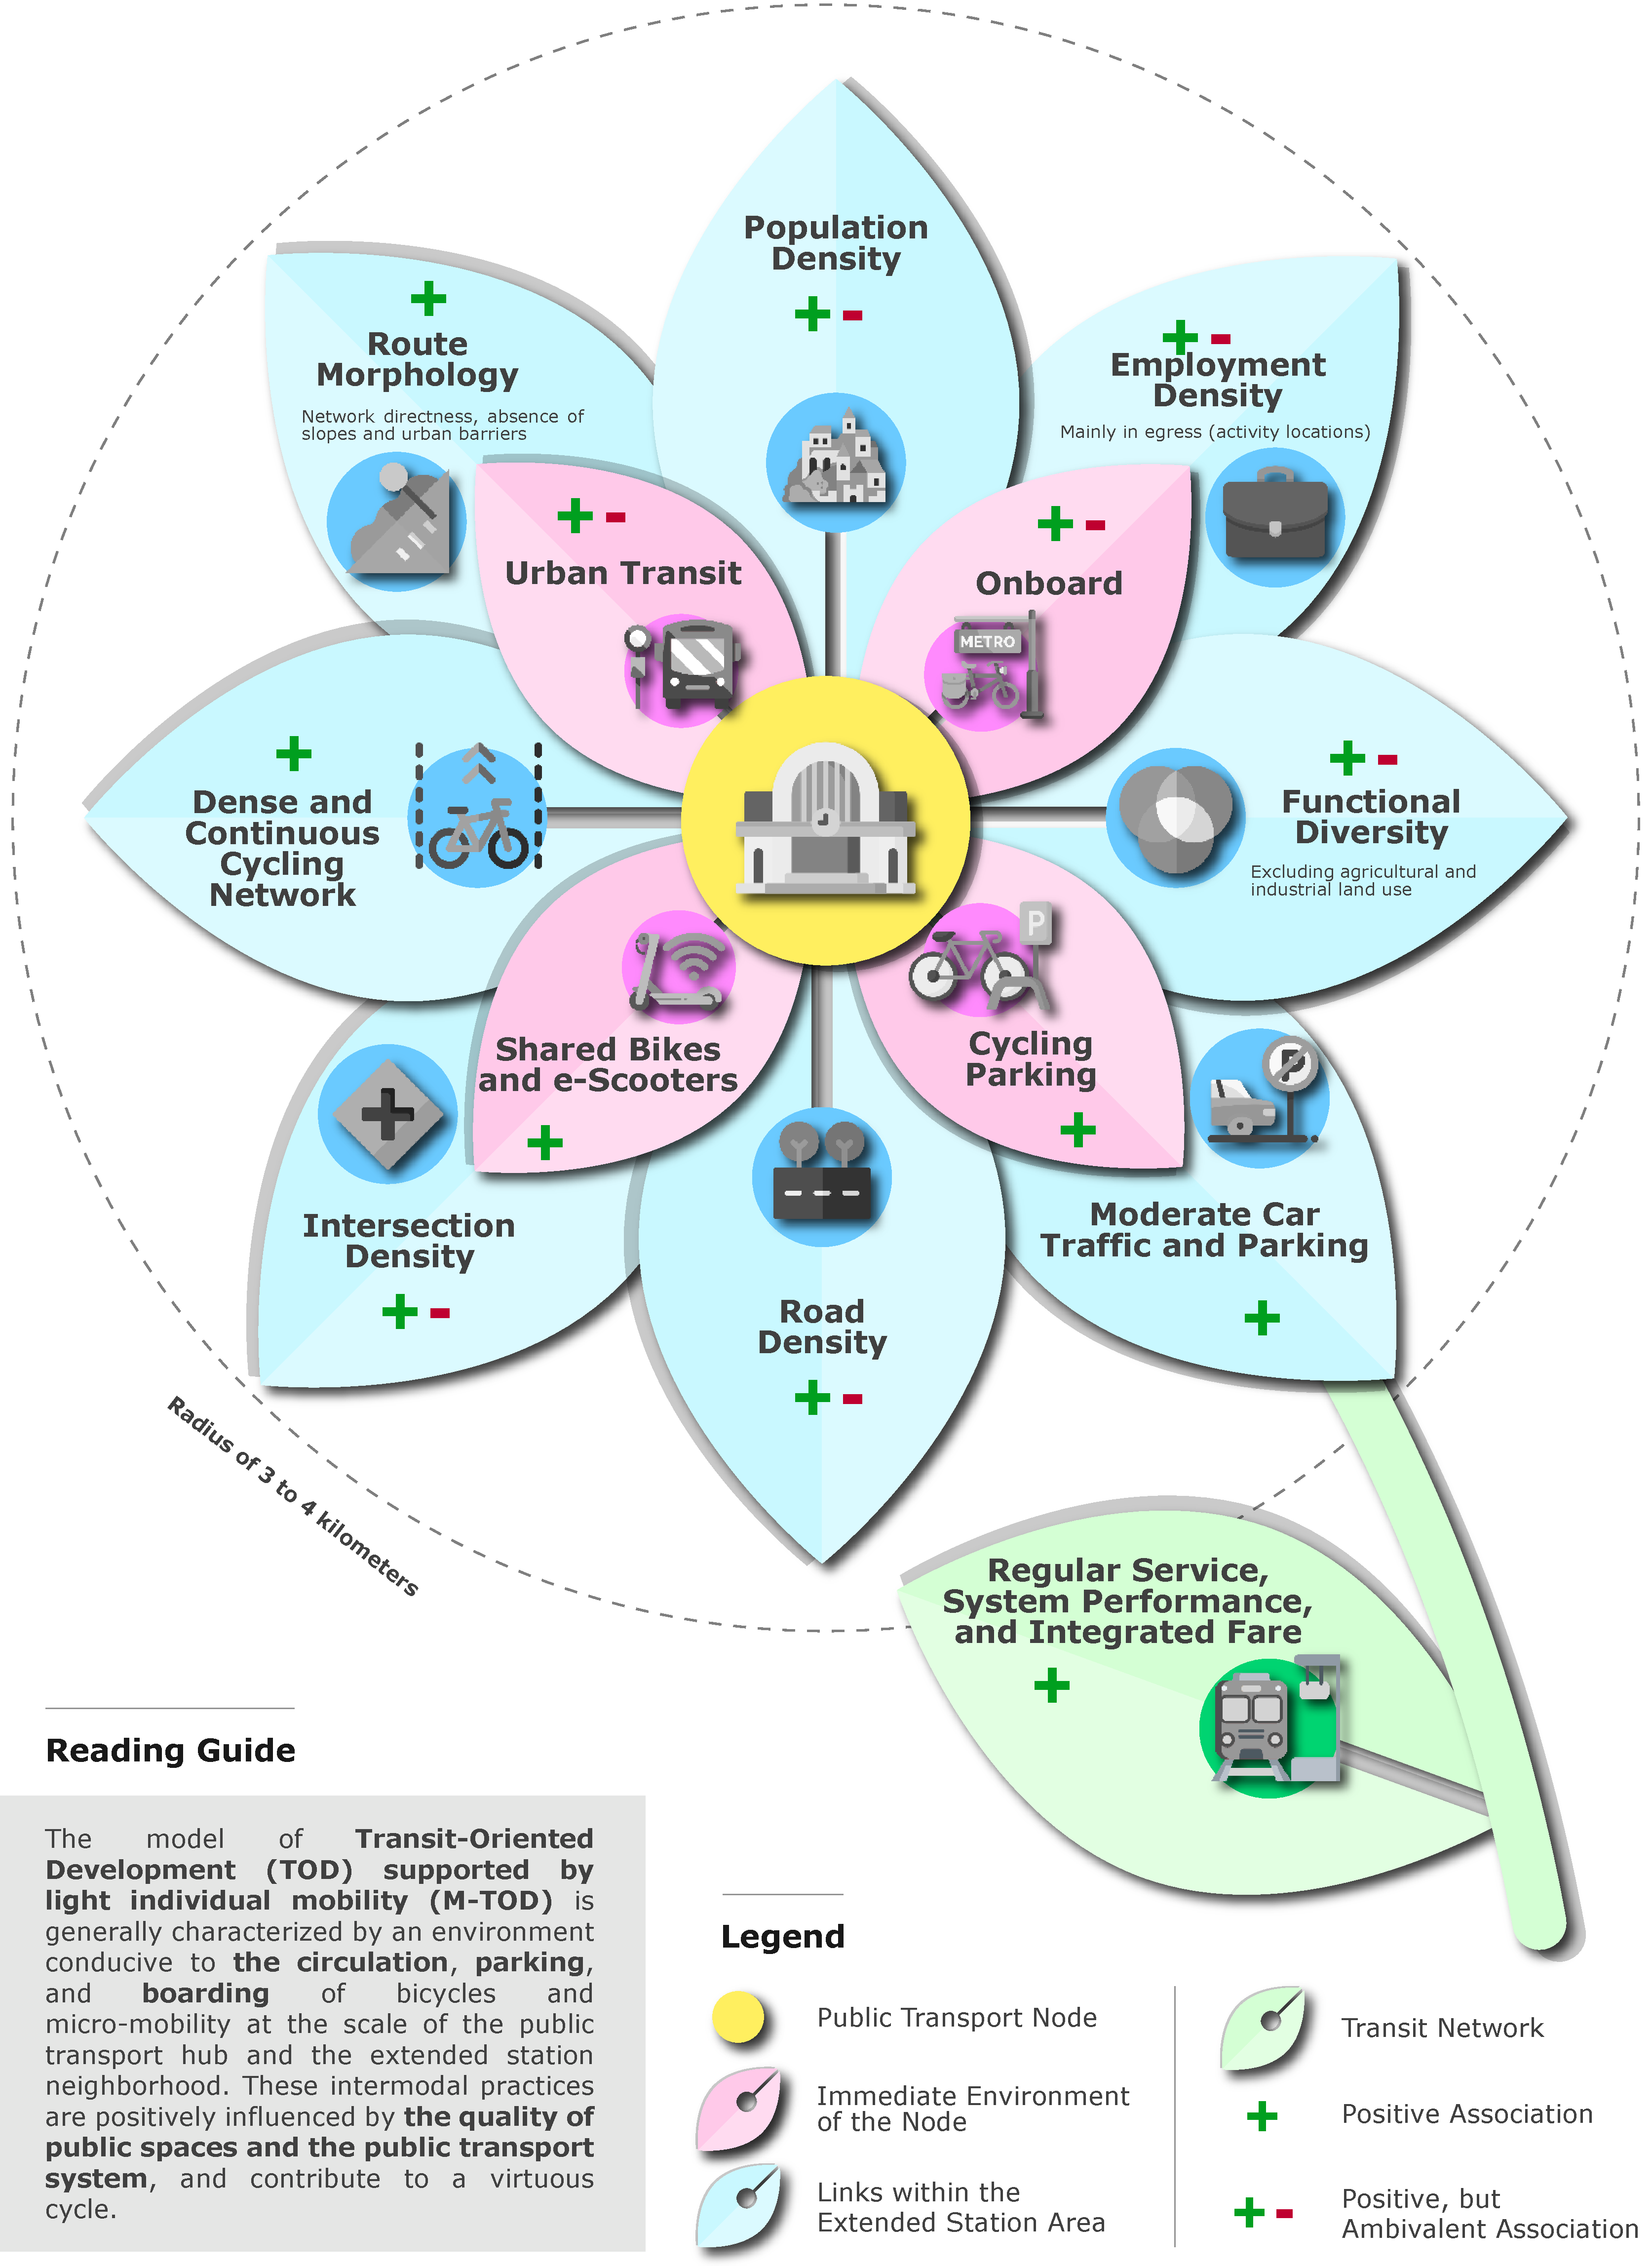
\includegraphics[width=1\columnwidth]{src/Figures/Chap-2/EN_RSL_Fleur_TOD.pdf}}
    \vspace{5pt}
    \begin{flushright}\scriptsize{
    Author: \textcolor{blue}{Dylan Moinse (2023)}
    }\end{flushright}
\end{figure}

% Objectifs
In response to the research questions posed in the \hyperref[chap2:formulation-questions-recherche]{Subsection~\ref{chap2:formulation-questions-recherche}} (page~\pageref{chap2:formulation-questions-recherche}), the goal of this \acrshort{SLR} lies in the ambition to deepen and expand the understanding of knowledge related to \acrshort{M-TOD}. This work aimed to clearly identify the factors that facilitate or hinder the adoption of this urban planning model. In this perspective, the analysis developed in this chapter was based on a set of six research questions, which served as the guiding framework for our study. These questions focus on the interaction between urban dynamics, public policies, and their role in integrating individual light mobility into public transport systems, as well as the influence of these practices on territorial configurations. The detailed examination of the literature highlighted the crucial importance of the \acrshort{7Ds} and mobility behaviors, offering a more nuanced and detailed perspective on these movements and their beneficial implications in the development of an urban model that promotes a sustainable and viable mobility and urban system. This study revealed that the extended influence area of train stations provides accessibility gains to a greater number of potential travelers. As a result, we can refer to the notion of \Commas{territorial reception potential} \textcolor{blue}{\autocite[86]{kaufmann_retour_2014}}\index{Kaufmann, Vincent|pagebf} as a key driver, supported by these mobility practices, linked to the principles of \acrshort{TOD}. In conclusion, the final research question addresses the challenges faced by this emerging urban model, particularly questioning the current gaps in the scientific literature in the face of recent knowledge production related to \acrshort{M-TOD}.%%Translated%%

% 2.*.*.*
\needspace{1\baselineskip} % Reserve space
\subsection*{Gaps in the Scientific Literature
    \label{chap2:literature-gap}
    }

    % Literature gap: state of the literature
As a transition towards the examination of our empirical material, we conclude this chapter by highlighting the main issues that still seem underexplored in relation to the concept of \acrshort{M-TOD}. The bibliometric analysis conducted in the context of our \acrshort{SLR} allowed us to identify various gaps related to the contours of our research topic. First, it is important to note an underrepresentation of studies considering certain forms of individual light mobility. Despite the growing interest in \acrshort{PBS}, \acrshort{DBS}, and \acrshort{DESS} since 2018, studies focusing on scooters and folding bikes, whether electric or non-motorized, remain relatively rare. This observation is accompanied by a focus on urban public transport systems, suggesting an untapped potential in the role of regional rail networks in association with new forms of mobility. Furthermore, we observe that the scientific and technical literature gives little attention to a systemic approach to the entire collective mobility system of a given geographic area, an approach that is crucial for understanding intermodal mobility in a systemic way. Moreover, the current scientific landscape reveals a geographical imbalance, with a predominance of studies set in international or regional agglomerations in China, the United States, and the Netherlands. Finally, the examination of the geographical frameworks studied shows a marked tendency to favor intercommunal and communal scales, while research adopting a regional scale remains exceptional.%%Translated%%

% Literature gap: concepts and methods
In light of the defined theoretical frameworks, we identified an interesting disparity between the frequent mention and use of the \acrshort{TOD} concept in the scientific literature and its near absence under the term \acrshort{M-TOD}. Regarding the research methods employed, we note a majority of studies relying on open or private databases derived from \textsl{Open Data} and \textsl{Big Data}. Furthermore, survey techniques such as questionnaires, interviews, or observations, which are generally more suited to medium-sized areas, are nonetheless equally present depending on the geographical contexts, particularly in Europe. However, it is worth noting the insufficiency of qualitative approaches and, more broadly, mixed methods research, especially concerning emerging individual light mobility options. The analysis methods suggest a strong inclination towards the use of modeling and descriptive statistics as well as \acrshort{GIS}.%%Translated%%

% Literature gap: results
The detailed analysis of the corpus constructed for this \acrshort{SLR} revealed not only disparities in the use of the \acrshort{7Ds} in connection with the \acrshort{M-TOD}, but also led to the development of new questions arising from the confrontation of empirical studies:
    \begin{customitemize}
\item What is the direct or indirect impact of population density on territorial configurations and the mobility practices favored by the \acrshort{M-TOD} urban model?
\item Is the notion of social mix complementary to the principles promoted by the \acrshort{M-TOD}?
\item Do the different forms of modal combinations induce specific needs in terms of infrastructure and cycling facilities?
\item What are the accessibility gains offered by the integration of individual light mobility within public transport systems?
\item How does the influence area of transport nodes vary according to the nature of modal combinations, the different stages of intermodal travel, and environmental and socio-demographic factors?
\item To what extent do the performance of public transport networks and the management of space dedicated to automobiles contribute to a better articulation between urban forms and mobility behaviors?
\item Can the \acrshort{M-TOD} be considered as a factor exacerbating mobility access inequalities?
\item Can this urban model integrate mobility related to leisure, social encounters, or walks (\textsl{undirected travel})?
\item Can the democratization of adopting individual light mobility in intermodality form a virtuous circle influencing urban forms, which, in turn, shape mobility behaviors?
    \end{customitemize}%%Translated%%

% Issues
In light of the challenges raised by the scientific literature regarding the design of an urban system oriented towards the development of public transport networks hybridized with the integration of individual light mobility, the doctoral thesis aims to better understand the key concepts of the \acrshort{M-TOD}. This chapter has highlighted the need to expand the research field on this topic to include a greater variety of mobility forms and levels of geographical analysis, in order to enrich our understanding of this urban planning strategy, reinterpreted through the lens of individual light mobility. These observations lead us to reflect on adopting a geostatistical approach combined with a qualitative methodology, which could provide more nuanced perspectives on individuals' mobility behaviors and experiences.%%Translated%%

% Thesis Structure
In this perspective, our doctoral research revolves around the exploration of a European geographic space at a regional scale, with particular focus on the entire mobility network, primarily structured around railway networks. The next \hyperref[chap3:titre]{chapter} (page~\pageref{chap3:titre}) will be dedicated to defining the geographic scope of the study and presenting our methodology, which includes a field survey. The goal of this mixed-method approach is to capture the development of intermodal practices that combine the use of public transport and emerging forms of individual light mobility, and to examine them in terms of mobility behaviors and their interactions with the urban environment (see \hyperref[chap4:titre]{Chapter~4}, page~\pageref{chap4:titre}). Identifying a social group of cycling commuters actively present in the various territories under study will allow us to explore their interactions in the context of expanded train station neighborhoods, using the concept of intermodal accessibility (see \hyperref[chap5:titre]{Chapter~5}, page~\pageref{chap5:titre}). This geographical approach to distances will lead us to propose a model based on a Node-Place Index, aimed at assessing the potential for urban development in synergy with an alternative mobility system at the regional scale, as outlined in \hyperref[chap6:titre]{Chapter~6} (page~\pageref{chap6:titre}).%%Translated%%

% ___________________________________________
     \newpage
     
% Valorisation scientifique
    \begin{tcolorbox}[colback=white!5!white,
                      colframe=blue!75!blue,
                      title=Valorization
                      \\
                      Chapitre~2]
\Large{\textbf{\textcolor{blue}{Book Chapter:}}}
    \\\\
\small{\textcolor{blue}{\textcite{moinse_systematic_2023}}\index{Moinse, Dylan|pagebf}. \foreignlanguage{english}{\textsl{A Systematic Literature Review on Station Area Integrating Micromobility in Europe: A 21\textsuperscript{st} Century Transit-Oriented Development}}. In: Belaïd,~F., Arora,~A. (eds) \textsl{Smart Cities. Studies in Energy, Resource and Environmental Economics}. Springer, Cham. ISBN: 978-3-031-35663-6 (p.~171-204).
\\
\footnotesize{\url{https://doi.org/10.1007/978-3-031-35664-3_12}} (\textbf{OS})}
    \end{tcolorbox}

    % ___________________________________________
    % Subbibliography
    \newpage
    \sectionheader{Bibliography of Chapter~2}
    \begingroup
    \renewcommand{\bibfont}{\scriptsize}
\printbibliography[segment=\therefsegment, heading=subbibintoc, title={Bibliography of Chapter~2}, label=chap2:bibliographie]
    \endgroup
    \end{refsegment}